\documentclass[a4paper,14pt]{extarticle}

\usepackage[T2A,T1]{fontenc}
\usepackage[utf8]{inputenc}
\usepackage[greek,french,english,russian]{babel}
\usepackage{csquotes}

\usepackage{pscyr}
%\usepackage[activate={true,nocompatibility},final,tracking=true,kerning=true,spacing=true]{microtype}
%% More avail. here: ht>tp://www.khirevich.com/latex/microtype/

%% Figure grids.
\usepackage{caption}
\usepackage{subcaption}
\renewcommand{\thesubfigure}{\asbuk{subfigure}}

%% PDF search & cut'n'paste
\usepackage{cmap}

%% Поля
\usepackage[foot=0pt,top=20mm,bottom=20mm,left=25mm,right=10mm]{geometry}

%% Отступ в первом абзаце
\usepackage{indentfirst}

%% Включение графических файлов.
\usepackage{graphicx}

%% Appendix.
\usepackage[titletoc,title]{appendix}
\renewcommand{\appendixtocname}{Приложения}
\renewcommand{\appendixpagename}{Приложения}
\renewcommand{\appendixname}{Приложние}
\makeatletter
\let\oriAlph\Alph
\let\orialph\alph
\renewcommand{\@resets@pp}{\par
  \@ppsavesec
  \stepcounter{@pps}
  \setcounter{section}{0}%
  \if@chapter@pp
    \setcounter{chapter}{0}%
    \renewcommand\@chapapp{\appendixname}%
    \renewcommand\thechapter{\@Alph\c@chapter}%
  \else
    \setcounter{subsection}{0}%
    \renewcommand\thesection{\@Alph\c@section}%
  \fi
  \if@pphyper
    \if@chapter@pp
      \renewcommand{\theHchapter}{\theH@pps.\oriAlph{chapter}}%
    \else
      \renewcommand{\theHsection}{\theH@pps.\oriAlph{section}}%
    \fi
    \def\Hy@chapapp{appendix}%
  \fi
  \restoreapp
}
\makeatother

%% Рисунки в приложении содержат номер приложения: 'A.1'.
\usepackage{chngcntr}

%% Russian-styled figure and table captions.
\usepackage[labelsep=period,font=it]{caption}

% Here we define the relationships for the counters: normaly we should
% reset the figure & table counters every chapter.
\makeatletter
\@addtoreset{figure}{section} % Figure counter
\@addtoreset{table}{section} % Table counter
\makeatother

%% Include paragraphis into TOC.
\setcounter{secnumdepth}{3}
\setcounter{tocdepth}{3}

%% Newline after paragrpaph title.
\makeatletter
\renewcommand\paragraph{%
   \@startsection{paragraph}{4}{0mm}%
      {-\baselineskip}%
      {.1\baselineskip}%
      {\normalfont\normalsize\bfseries}}
\makeatother

%% Drop chapter number and
% \usepackage{titlesec}
% \renewcommand{\thesection}{\arabic{section}}
% \renewcommand{\thesubsection}{\arabic{subsection}}

\usepackage[titles]{tocloft}

%% Inline-списки.
\usepackage{paralist}
\usepackage[inline]{enumitem}
\AddEnumerateCounter{\asbuk}{\@asbuk}{\cyrm}

\makeatother
\renewcommand{\labelitemi}{--}

% Keeps floats `in their place', preventing them from floating past a
% "\FloatBarrier" command into another section.  The floats should not move
% past every "\section".
\usepackage[section]{placeins}

\usepackage[%
    backend     = biber,
    bibencoding = utf8,
    hyperref    = false,
    babel       = other,
    citestyle   = gost-footnote,
    bibstyle    = gost-numeric,
    citereset   = section
]{biblatex}
\addbibresource{references/chapter1.bib}
\addbibresource{references/chapter2.bib}
\addbibresource{references/conclusion.bib}

%% Ссылочки.
\usepackage{hyperref}
\makeatletter
\let\abx@macro@autociteOrig\abx@macro@autocite
\renewbibmacro{autocite}{%
   \bibhyperref{%
   \let\bibhyperref\relax\relax%
   \abx@macro@autociteOrig%
   }%
}%
\makeatother

%% Separate multiple cites with '; '
\renewcommand\multicitedelim{\addsemicolon\space}

\usepackage{remreset}
\makeatletter\@removefromreset{footnote}{chapter}\makeatother

%% Полуторный интервал
\usepackage[nodisplayskipstretch]{setspace}

%% Переименование "содержания" в "оглавление"
\gappto\captionsrussian{\renewcommand{\contentsname}{Оглавление}}

\addtolength{\textheight}{\headheight}
\addtolength{\textheight}{\headsep}
\setlength{\headsep}{0pt}
\setlength{\headheight}{0pt}

%% Преобразует footnote '2 3' -> '2, 3'.
\usepackage[multiple]{footmisc}

\usepackage{fancyhdr}
\fancyhf{} % clear all header and footers
\renewcommand{\headrulewidth}{0pt} % remove the header rule
\fancypagestyle{plain}{
\fancyhead[C]{\thepage}}
\pagestyle{plain}

\usepackage{hyphenat} 

\setlist[1]{topsep=0pt,parsep=0pt,itemsep=0pt}

\begin{document}
% ------------------------------------------------------------------------------
% Титульный лист
\thispagestyle{empty}

\begin{center}
  Федеральное государственное бюджетное образовательное учреждение высшего профессионального образования \\
  <<Костромской государственный университет имени Н. А. Некрасова>> \\
  \vspace{1em}
  Кафедра теории и истории культур
\end{center}
\vspace{.1em}
\begin{flushright}
  \textit{На правах рукописи} \\
  \vspace{14pt}
  
\includegraphics[width=2.9cm]{images/lebedev}
\end{flushright}
\begin{center}
  \textbf{ЛЕБЕДЕВ Никита Андреевич} \\
  \vspace{3em}
  \textbf{ЛОГОТИП КАК ФОРМА МАССОВОГО СОЗНАНИЯ:\\
    СТРУКТУРА, ФУНКЦИИ, ЭМБЛЕМАТИКА} \\
  \vspace{3em}
  Специальность 24.00.01 – теория и история культуры \\
  \vspace{3em}
  \textbf{Диссертация} \\
  на соискание ученой степени \\
  кандидата культурологии
\end{center}
\vspace{3em}
\begin{flushright}
  Научный руководитель: \\
  доктор культурологии, \\
  профессор И. А. Едошина
\end{flushright}

\vspace{6em}
\begin{center}
  Кострома 2013
\end{center}


% ------------------------------------------------------------------------------
% Оглавление
%\microtypesetup{protrusion=false}
\thispagestyle{empty}             % Disables numbering on the TOC page.
\tableofcontents
%\microtypesetup{protrusion=true}

% ------------------------------------------------------------------------------
% Текст работы
\begin{onehalfspace}
\addcontentsline{toc}{section}{Ввдение}
\section*{Введение}

\textbf{Актуальность исследования} определяется необходимостью дифференцированного изучения эмблематической природы логотипа в культурном пространстве современности. Сознание человека информационного общества подвержено активному воздействию различных знаков. Изучение информации, заложенной в эти знаки, поможет глубже понять экзистенциальную ситуацию современного человека и то время, в котором он живёт. Если классическая культурная традиция, по определению постмодернистских философов, логоцентрична (Деррида, Фуко), то современная культура скорее логотипична, чем логоцентрична. Традиционные культурные знаки, символы и эмблемы все чаще переформулируются в медийном дискурсе в терминах коммерческой деятельности и называются логотипами. Национальный флаг, герб суть логотипы. Есть общепринятые эмблемы-логотипы стран и городов, как, например, «большое яблоко» Нью-Йорка или «сапожок» Италии. А логотип-слоган «I love NY», разработанный в середине 1970-х американским графическим дизайнером Милтоном Глейзером, является одной из самых популярных коммерческих икон современности. Другими словами, логотип перешёл из сферы товарных взаимоотношений в сферу культуры в целом. Логотипы окружают нас в цифровом и физическом пространстве, однако, в повседневной жизни мы редко задумываемся о культурной составляющей логотипа. Логотип в культурно-исторической перспективе – это значимый артефакт, поскольку он документирует человеческую историю, историю вещей, историю потребления.

Актуальность данного исследования определяется следующими \textbf{противоречиями:}
\begin{itemize}
\item между недостаточной изученностью процессов визуализации культуры и понимания суггестивных механизмов воздействия логотипов, формирующих и отражающих современное сознание;
\item между большим количеством ненаучных подходов к пониманию сущности логотипа и недостаточной разработанностью научно-методической базы;
\item между массовыми процессами брендирования в современной культуре и утратой личностного начала в человеке.
\end{itemize}

Выявленные противоречия дают основание сформулировать \textbf{научную проблему} исследования: какие стороны в современной культуре отражает и формирует логотип.

\textbf{Степень научной разработанности проблемы}

Среди источников по исследуемой теме – работы культурологов, философов, историков, семиотиков, психологов и др., изучающих концепты «массовое сознание», «массовое общество», «массовая культура» и др.

Так, в семиотической области диссертант опирался на труды Р. Барта, Ж. Бодрийяра, М.К. Голованивской, Е. Горного, Е. Григорьевой, Э. Кассирера, Ю.М. Лотмана, Ч. Морриса, Ч. Пирса, А.Б. Соломоника, Ф. де Соссюра, Б.А. Успенского, Л.Ф. Чертова, У. Эко.

Культурологический аспект находит своё отражение в работах, посвященных проблемному полю массовой культуры А.Я. Гуревича, И.А. Едошиной, В.С. Елистратова, И.В. Кондакова, М.И. Найдорфа, К.Э. Разлогова, Н.В. Серова, Е.Г. Соколова, Г.Л. Тульчинского, Р. Уильямса, Й. Хёйзинги.

Важную роль сыграли работы французской историографической школы «Анналов»: М. Блока, Ф. Броделя, Ж. Ле Гоффа, Л. Февра.

При описании теоретических исследований современного общества учитывались работы социологов: Х. Арендт, Д. Белла, Г. Блумера, М. Вебера, Г. Зиммеля, У. Корнхаузера, Ю.А. Левады, Э. Ледерера, Д. Макдональда, Л. Мамфорда, К. Маннгейма, Г. Маркузе, Х. Ортеги-и-Гассета, Б.Ф. Поршнева, Д. Рисмена, Г. Тарда, А. Тоффлера, Э. Фромма, Э. Шилза, Ф. Юнгера и других.

Философский аспект представлен работами М.М. Бахтина, Г. Гегеля, А. де Боттона, А.Н. Ильина, Л.Г. Ионина, А.Ф. Лосева, М. Маклюэна, М.К. Мамардашвили, П.А. Флоренского, М. Фуко, Р.У. Эмерсона и других.

Психологический подход представлен работами В.М. Бехтерева, Л.И. Божович, Р. Броуди, П.Я. Гальперина, Л.С. Выготского, А.А. Леонтьева, А.Н. Леонтьева, Г. Лебона, А.Р. Лурии, Д.В. Ольшанского, В.С. Рамачандрана, З. Фрейда, Д.А. Эльконина, К.Г. Юнга и других.

Из известных авторов, пишущих о логотипе как о предмете научного анализа, можно выделить Ж.-Л. Азизола, Э. Амиот, Д. Боуи, К. Дж. Веркмана, Б. Гарднера, Л. Кабарга, М. Макнаб, П. Моллерапа, С. И. Серова, Б. Эльбрюнна и ряд других. Феномен логотипа, в силу своего весьма специального характера, связан либо с решением инструментальных задач графического дизайна (Ю. Гордон, Я. Чихольд), либо с изучением логотипа в рамках экономических наук (С. Анхольт, К. Динни, Н. Кляйн, Ф. Котлер, М. Линдстром, А. Уиллер и др.). При этом культурологическое осмысление логотипа пока остаётся вне поля внимания специалистов.

Указанные исследования в общей сложности составляют солидную теоретическую базу, позволяющую системно изучить логотип как форму массового сознания, его структуру и социокультурное назначение.

\textbf {Целью исследования} является представление логотипа как формы современного массового сознания, обладающей структурой, имеющей определённые функции и отличающейся эмблематической природой.

\textbf {Объектом} исследования выступает логотип как инструмент формирования и отражения массового сознания.

\textbf {Предметом исследования} является логотип как форма современного массового сознания, его структура, функции и отличающуюся эмблематической природой.

\textbf{Гипотеза исследования}: логотип является формой иконической репрезентации современного массового сознания и отражением его ментальности.

Массовое сознание отличается от других форм общественного сознания специфическими свойствами его носителя, т.е. массы. В частности – массы потребителей. Логотип, будучи формой массового сознания, с одной стороны, отражает его основные социально-психологические свойства. К таковым относятся визуальная зависимость, мозаичность, эмоциональность, заразительность, изменчивость и подвижность. С другой стороны, он выполняет функцию управления содержанием сознания массового потребителя и его потребительской активностью.

Структурно логотип представляет собой соединение визуальных и вербальных составляющих, образующих единый смысловой комплекс, подобно эмблеме.

Эмблематическая сущность логотипа заключается в выполнении им мнемонической функции. Иначе говоря, логотип представляет собой готовый блок памяти, внедряемый в массовое сознание. Основная задача такого блока состоит в том, чтобы, во-первых, заложить в долговременную память симулятивные образы и установки на потребление. Во-вторых, обеспечить их быстрое извлечение из памяти в каждой конкретной ситуации потребления.

Высшей точкой семантической эволюции логотипа в сознании массового человека-потребителя следует считать бренд, под которым понимается статусный символ-икона современного массового общества.

Данная цель реализуется в ряде основных \textbf {задач}:
\begin{enumerate}
\item На основе изучения ментальности массового общества выявить её культурно\hyp{}семиотические параметры.
\item Представить сознание человека массы как объект знаковой манипуляции.
\item Обозначить культурно-значимые тенденции в современном лого дизайне.
\item Используя классификационный подход, представить логотип как культурный артефакт, отражающий сознание массового человека.
\item Определить эмблематическую сущность логотипа и выявить суггестивные механизмы воздействия логотипов на современное массовое сознание.
\end{enumerate}

\textbf{Методологическая база исследования}
Выбор методологии обусловлен намеченными задачами и поставленной целью. В основе исследования применён структурно-функциональный метод, который определён знаковой природой логотипа и спецификой современного сознания, часто опирающегося на визуализацию. Этот метод позволил рассмотреть не только практическое решение и разработку логотипов в графическом дизайне, но прежде всего – внутреннее смысловое содержание логотипа как знака современной визуальной культуры.

Кроме того, в диссертационном исследовании задействован дескриптивный метод, позволяющий не только дифференцировать логотип как культурный феномен, но и представить его как некое культурное единство на основе понятий «массовое сознание», «ментальность», «массовое общество», «массовая культура», «знак», «логотип», «бренд».

Для истолкования фактов практики лого дизайна в исторической перспективе применён сравнительно-исторический метод.

Для получения актуальной информации по проблемным вопросом исследования в диссертации использован метод интервью (Было проведено интервьюирование современных специалистов в сфере лого дизайна).

В работе используются также и традиционные методы теоретического исследования: анализ, синтез, индукция, дедукция, реферирование, научная классификация.

\textbf{Хронологические рамки} исследования определяются концом XX – началом XXI в.

\textbf{Источниковой базой исследования} послужили труды отечественных и зарубежных специалистов в области визуальной культуры: культурологов, историков, семиотиков, социологов, психологов, маркетологов, рекламистов; словари и справочники; классификации-сборники логотипов.

\textbf{Научная новизна исследования:}
\begin{enumerate}
\item Логотип впервые представлен как форма современного массового сознания, определены его функции, выявлена эмблематическая природа.
\item Предпринята попытка комплексного культурологического анализа логотипа в массовой культуре. Именно благодаря культурологическому подходу удалось синтезировать и творчески использовать теоретические исследования из семиотики, психологии, философии, социологии, маркетинга и других областей знания. Разработанный базис может быть использован для дальнейшего более подробного и более специализированного изучения феномена логотипа.
\item Выявлены отдельные культурно значимые тенденции современного массового общества, например, массовое брендирование. Если логотип является визуальным знаком потребительской ориентации в массовой культуре, то бренд можно считать знаком-эталоном качества, престижа и статуса в сознании массового потребителя. Бренды формируют особый культурный код или язык в современной массовой культуре. В частности, интерес представляют процессы территориального брендирования, под которыми понимается массовое переназывание и символическое визуальное переосмысление устоявшихся знаковых обозначений традиционной культуры и национальной идентичности. Другой тенденцией в эволюции современного массового сознания является практика индивидуального самобрендирования по образцу формирования корпоративной идентичности в сфере экономической деятельности. Визуальная самоидентификация через обладание персональным лого становится неотъемлемой частью самобрендирования.
\item Доказано, что в сфере потребления по своему замыслу и основному символическому назначению логотип, подобно эмблеме, является свернутым мнемоническим блоком, призванным, с одной стороны, транслировать уникальный ценностный статус компании-производителя и ее продукции, а, с другой стороны, внушать целевому массовому потребителю ощущение эмоциональной сопричастности некоему симулятивному таинству или псевдо-мистическому опыту, будь то коммерческая утилизация древних символов или маркетинговая мифологизация нового технологического чуда.
\end{enumerate}

\textbf{Теоретическая значимость} исследования состоит в том, что его результаты синтетически обобщают имеющиеся знания о логотипе и вносят вклад в создание теории логотипа на культурной платформе. Разработаны методологические подходы к уточнению форм бытийствования массового сознания. Скорректировано понимание знаковой природы современного массового сознания. Знание форм иконической репрезентации массового сознания позволяет расширить понятийную базу культурологических исследований и углубить понимание процессов и феноменов массовой культуры. Помимо этого, такой подход позволяет выявить интегративную природу культурологической рефлексии, уточнить некоторые характеристики культурологического метода, в частности, как это показано на примере массовизации управляемых процессов по формированию бренд-идентичности.

\textbf{Практическая значимость} заключается в выявлении форм массового сознания и механизмов влияния на него. Знание этих механизмов может быть использовано в прикладной культурологии, в частности, в семиотическом маркетинге, принципах разработки брендов. Полученные данные также могут быть применены в курсах по культурологии, истории культур, межкультурной коммуникации, семиотике, а также в рамках курса графического дизайна и брендинга.

\textbf{Апробация результатов диссертационного исследования}

Основные результаты исследования обсуждались на занятиях по специальности, на заседаниях кафедры теории и истории культур Костромского государственного университета (2010–2013 гг.), апробировались в докладах и тезисах на международных, региональных и межвузовских научных конференциях: «Костромская земля: памятники культуры малых городов» (Кострома, 2011); «Женские мотивы и образы в культуре русской провинции» (Кострома, 2012); «Культура земли Костромской: традиции и современность» (Кострома, 2012); «Актуальные проблемы современного российского общества: традиции и новации» (Кострома, 2012); «Сапоговские штудии. Современное гуманитарное знание в России» (Кострома, 2012); «Актуальные вопросы культурологии, истории и филологии» (Кострома, 2012); «Пропилеи на Волге 2013. Кавказ и русская культура» (Кострома, 2013).

\textbf{Положения, выносимые на защиту:}
\begin{enumerate}
\item Логотип есть форма современного массового сознания. По своей сути логотип ориентирован на массовое сознание и потребление. Он не только отражает или выражает массовое сознание, но и формирует его.
\item Структурно логотип есть иконический знак, основанный на синтезе вербальных и невербальных элементов. По способности обобщения логотип является эвристическим знаком-символом, формирующим позитивный имидж компании. По способности отражения сегментов реальности логотип конвенционален и условен. По функциональному назначению логотип есть коммерческий знак-образ.
\item Помимо своих основных функций (идентификационная, рекламная, информационная), логотип выполняет ещё и идеологическую функцию, транслируя массовые общественные ценности и ориентиры. Основная смысловая нагрузка, возлагаемая на логотип в современной культуре и массовом сознании – это придание высокого статуса компании производителю и ее продукции, с одной стороны, и потребителю продукции компании, с другой.
\item Логотип предполагает манипуляцию массовым сознанием с использованием внешних и внутренних форм суггестии. При этом внешние формы возможны благодаря повсеместному использованию логотипов-эмблем на различных носителях, а внутренние основаны на приёмах аффектации и обращении к образам и паттернам коллективного бессознательного.
\item Логотип может быть уподоблен эмблеме по структурной сочетаемости изобразительных и вербальных элементов. Логотип, понимаемый как эмблематическое сочетание, подвержен энтропии, т.е. распаду фиксированного смысла, традиционно присущего эмблеме.
\item В культурно-исторической перспективе логотип является артефактом культуры, отражающим ментальность людей, их потребительские привычки и вкусы.
\end{enumerate}

\textbf{Личный вклад} автора работы заключается в том, что впервые предпринята попытка культурологического исследования логотипа как формы массового сознания и феномена массовой культуры. Выявлена эмблематическая сущность логотипа, определены его функции и структура.

Комплексное изучение логотипа представляет собой анализ следующих аспектов:
\begin{enumerate}
\item Психологический аспект заключается в учёте особенностей человеческого восприятия образа, формы, цвета, композиции и т.д.
\item Семиотический аспект выражается в том, что эффективность воздействия знака может быть усилена через использование культурно насыщенных знаковых комплексов и символов.
\item Культурологический аспект представлен эвристическим анализом культурно\hyp{}значимых контекстов, таких как традиционные вкусовые предпочтения массового потребителя с учётом социокультурного признака, национальных и временных особенностей. Историко-культурологические классификации, представленные в работе, наглядно демонстрируют, как логотип отображает ментальность, потребности и нравы массового человека в определённую временную эпоху. Анализ тенденций в лого дизайне позволяет увидеть, насколько быстро меняются предпочтения потребителя, его стремления и чаяния. Подобно сущностным характеристикам массового сознания, эти тенденции не регламентируемы и носят спонтанный, диффузный характер.
\end{enumerate}

\textbf{Соответствие диссертации паспорту научной специальности}

Работа соответствует специальности 24.00.01 «Теория и история культуры» и выполнена в соответствии со следующими пунктами паспорта специальности ВАК: 1.21 – традиционная, массовая и элитарная культура; 1.23 – личность и культура; 1.24 – культура и коммуникация; 3.21– социокультурные последствия коммерциализации культуры; 3.6 – «массовая культура» как социальный феномен.

\textbf{Структура диссертации}

Диссертационное исследование состоит из введения, двух глав, шести параграфов, заключения, библиографического списка использованных источников и литературы общим объемом 211 наименований, 10 приложений, включающих таблицы и рисунки. Содержание диссертации изложено на 180 страницах. Общий объём работы 256 страниц.

\section{Генезис логотипа}\label{chapter1}

\subsection{Ментальность массового общества: семиотический аспект}\label{1}
Развитие рыночной экономики, индустриализации, демократизация технологий в ХХ веке закономерно привели к этапу развития цивилизации, который принято называть массовым обществом и массовой культурой. На сегодняшний день в культурологии нет единого мнения относительно того, что следует считать массовой культурой и где проходят ее временные границы. В современном русском языке слово «массовая культура», как правило, имеет негативную коннотацию и употребляется скорее как оксюморон, в котором отрицательное значение слова «массовый» «гасит» положительное значение слова «культура» \autocite{elistratov2012}. При таком подходе «массовая культура» - это циничное манипулирование гомогенизированными массами и игра на их первичных инстинктах. Между тем, массовая культура окружает нас со всех сторон, она растёт по экспоненте, неудержимо проникает во все уголки нашей жизни. Претензии к массовой культуре традиционно ограничиваются критикой сравнительно незначительной ее части – массового искусства. В значительной же для жизни каждого человека сфере культуры, названной Ф. Броделем структуры повседневности, большинство форм и предметов массовой культуры не только не  осуждаются, но всячески приветствуются. В аспекте «структур повседневности» массовая культура способна обеспечить большинству населения «достойную жизнь» - возможность красиво одеваться, вкусно питаться, путешествовать, обустраивать свой дом, всемерно удовлетворять все возрастающие потребности. Понятно, что такая культура получает всестороннюю поддержку на всех уровнях общества. Именно в модусе «структура повседневности» массовой культуры функционирует логотип, семиотически организующий пространство массовой потребительской деятельности людей и визуально формирующий символическую среду нашей феноменально-актуальной телесности. Последовательно рассмотрим термины: \emph{массовое общество}, \emph{ментальность},
\emph{семиотика}\autocite{society}.

\subsubsection{Рабочие границы терминов \emph{массовое общество}, \emph{ментальность}, \emph{семиотика} в культурологии}\label{1.1}
\paragraph{Массовое общество}\label{1.1.1}

В культурологии массовое общество принято называть обществом потребления, «в котором “иметь” равносильно тому, чтобы “быть”»\autocite[][199]{razlogov2005}. Массовое общество – закономерный продукт масштабных социально-политических  и производственных процессов в западной и отечественной культуре ХХ века. Главный герой столетия – “средний”, “массовый” человек, оказавший серьёзное, формообразующее воздействие «на все процессы и перемены, от производства до войн, от системы ценностей и социальной мифологии до спорта и досуга» \autocite{levada2001}. Первым понятие массы ввел в научный дискурс французский психолог Г. Лебон, рассматривавшего толпу (массу) в качестве психологического феномена, возникающего при прямом взаимодействии индивидов, независимо от их социального статуса, рода деятельности или национальности. По его мнению, в толпе формируется некое социально-психологическое единство массы, наделенное общими чувствами, взаимовнушением, высоким уровнем энергетики, нейтрализующими сознательную личность. К более поздним серьезным и разноплановым теоретическим исследованиям массового общества, написанным главным образом в 20-60-е годы ХХ века, можно было бы отнести работы Габриеля Тарда, Георга Зиммеля,
Макса Вебера, Карла Маннгейма, Эмиля Ледерера, Герберта Блумера, Дэвида Рисмена,
Даниеля Белла, Хорхе Ортеги-и-Гассета, Ханны Арендт, Льюиса Мамфорда, Фридриха Юнгера,
Эриха Фромма, Герберта Маркузе, Уильяма Корнхаузера, Жана Бодрийяра, Эдварда Шилза и др. Д.В.~Ольшанский в своем историческом экскурсе\autocite[][15]{olshansky}
перечисляет семь таких подходов:
\begin{enumerate}[label={\arabic*)}]
    \item как толпа (традиции Г.~Лебона);
    \item как публика (последователи Г.~Тарда);
    \item как гетерогенная аудитория, противостоящая классам и относительно гомогенным
    группам (Э.~Ледерер и Х.~Арендт, например, считали массы продуктом дестратификации
    общества, своего рода \emph{антиклассом});
    \item как \emph{агрегат людей, в котором не различаются группы или индивидуумы} (У.~Корнхаузер);
    \item как уровень некомпетентности, как снижение цивилизации (X.~Ортега-и-Гассет);
    \item как продукт машинной техники и технологии (Л.~Мамфорд);
    \item как \emph{сверхорганизованное} (К.~Маннгейм) бюрократизированное общество,
    в котором господствуют тенденции к униформизму и отчуждению.
\end{enumerate}

В сущности, список можно с легкостью продолжить, добавив, например, постмодернистскую
трактовку Ж.~Бодрийяра, к чьим работам мы будем неоднократно обращаться позднее.
Бодрийяр, как известно, ввел альтернативный термин для описания массы (\emph{молчаливого большинства}) --
\emph{общество потребления}, эволюции массового общества на новом историческом этапе.
В книге <<В тени молчаливого большинства, или Конец социального>>~\autocite{book:bodriyar} он, в частности,
утверждает, что масса -- это разновидность \emph{черной дыры}, падение в самих в
себя, которое не обладает ни атрибутом, ни предикатом, ни качеством, ни референцией.
Масса, по Бодрийяру, радикально неопределима и не имеет социологической реальности.
Она не является ни субъектом истории, ни ее объектом.

В отечественной гуманитарной традиции проблемы массового общества с разных сторон освещались П.С. Гуревичем, А. Н. Николюкиным, К.Э. Разлоговым, Л.Г. Иониным, Ю.А. Левадой, Г. Л. Тульчинским, М.И. Найдорфом, А.И. Ильиным, Е.Г. Соколовым и др. Так, А. И. Ильин считает, что термин <<массовое общество>> содержит в себе внутренне противоречие, По его мнению, существовать может только либо масса, либо общество, но никак не массовое общество. В тоже время, как масса, так и общество «находят свое одновременное существование (сосуществование) как субъекты массовой культуры»\autocite[][79]{ilin2010}. Соответственно, массовое общество, полагает Ильин, представляет собой «социальное пространство, содержащее внутри себя как массу бессубъектных индивидов, так и общество как находящуюся на более высоких ступенях культурного развития совокупность субъектов»\autocite[][79]{ilin2010}.

В данной работе мы, во-первых, исходим из того представления, что массовое общество – это такая форма общности, в которой «отчетливо проявился “человек массы” как носитель особого типа сознания – массового сознания»\autocite[][289]{kagan2007}. Появление человека массы, как убедительно доказывал Ортега-и-Гассет в “Восстании масс”, следует рассматривать как закономерный результат предшествующего развития новоевропеской социокультурной традиции. Во-вторых, ниже мы не делаем специального различия между терминами “массовое общество” и “массовая культура” и используем их взаимодолнительно. Вслед за Е.Г. Соколовым\autocite{sokolov2002}, мы понимаем под массовой культурой такую культурную ситуацию, которая соответствует рыночной форме социального устроения общества\autocite[][20]{edoshina2000}. Это культура «в присутствии Масс»\autocite[][289]{kagan2007}.

\paragraph{Ментальность}
\label{mentality}
Ментальность принято считать основной характеристикой феномена сознания\autocite[][52]{edoshina2000}. Более широко: в отечественной теоретической культурологии под ментальностью предлагается понимать «глубинный уровень коллективного и индивидуального сознания, включающий и бессознательное; относительно устойчивая совокупность и предрасположенностей индивида или социальной группы воспринимать мир определенным образом»\autocite[][414]{razlogov2005}.

Понятие о коллективных представлениях детализировалось и получило развитие в трудах Э. Фромма~\autocite{book:davydov}, Г. Бутуля,
Л. Февра и М. Блока~\autocite{book:febvre}, Э. Ле Руа, Ж. Ле Гоффа,
М. Фуко~\autocite{book:arch}, К. Г. Юнга~\autocite{book:yung},
Й. Хейзинги~\autocite{book:heizenga}, Г.-В. Гетса, Ф. Броделя  и др. Среди российских ученых, внесших вклад в изучение ментальности следует отметить труды М. М. Бахтина~\autocite{book:tamarchenko}, А. Я. Гуревича, Ю. Л. Бессмертного, А. Л. Ястребицкой, В. П. Даркевичa\autocite{levit1998}, А.С. Мыльникова\autocite{milnikov1996}, В. П. Визгина, Н. В. Кондакова, Л.В. Санжеевой\autocite{sanjeeva2011} и др.

В самом общем виде \emph{ментальность} культурологически определяется как
видение мира и его восприятие, образ мысли и нормы поведения, в которых сочетаются
сознательные и бессознательные моменты. Ж. Ле Гофф, в частности, подчеркивает неизбежно коллективный характер ментальности, т.е. того общего, что «индивид разделяет с другими людьми своего времени … на уровне повседневного автоматизма поведения»\autocite{sharte2004}. Ниже мы будем отталкиваться от родственного определения ментальности: «ментальность есть сама психология, взятая в контексте социальных условий; это обыденность, средний человек и способы чувствования, мышления, силы, формирующие привычки, отношения, безличный культурный контекст»\autocite{online:kulturolog}.

Иначе говоря, в самой идее ментальности синкретично соединяются характеристики психологической и непсихологической (культурной и социальной) реальностей. При этом ментальность, так или иначе, находит свое выражение в повседневной жизни людей. А поскольку повседневностью живет все-таки каждый человек, то категория «повседневности» в данном случае будет служить краеугольным камнем в нашем исследовании. По Ф. Броделю, повседневность внеисторична, расплывчата, неопределенна и неопределима. Тем не менее, к ее организующим принципам можно отнести, во-первых, иерархичность (верхи и низы). Низовым уровням присущи стабильность, консерватизм, устойчивость к переменам. Элита, верхи общества, определяют ценностные ориентиры и создают иерархические порядки. Во-вторых, понятие стиля или стилизации. При этом стиль, как некая культурная целостность, влияет как на материально-предметный мир, так и на поведенческие нормы, проявлясь в речи, манерах и пр. В-третьих, категорию времени и пространства. Логотип, как мы покажем, в полной мере соответствует критериям повседневности и как таковой обладает мощным потенциалом влияния на ментальность стихийных массовых сообществ, социальных групп и общества в целом.

\paragraph{Семиотика}\label{1.1.3}

Хотя литература по семиотике обширна, ее институциональный статус по-прежнему не определен.~\autocite{sirotkin}
Более того, современная семиотическая теория на данный момент также не имеет ни
единой методологии, ни общей теории.~\autocite{gorny}\autocite{gasparov}. Консенсус есть только в понимании семиотики как науки о знаках и знаковых системах. Знак -- это инструмент (или орудие),
с помощью которого решаются две основные задачи:
\begin{inparaenum}[\itshape 1\upshape)]
    \item быстрого получения, передачи, переработки и
    \item надежного хранения знаний/информации в обществе.
\end{inparaenum} Или же, в определении Ю.М.~Лотмана: ``Знак -- это материально выраженная замена предметов, явлений, понятий в процессе обмена информацией в коллективе.''~\autocite{wiki:symbol}
Здесь, по-видимому, следует сделать важное уточнение. Знаком заменяется не столько сам
обозначаемый предмет, взятый в своей целокупности, сколько его отдельные свойства или
качества, метонимически представляющие его целостность в индивидуальном и коллективном сознании. Отсюда естественным образом вытекает важнейшая ценностная образующая знака -- его значение. Помимо указания на предмет, значение знака есть не что иное, как наше представление об означаемом предмете, коллективно признанное и индивидуально осознанное. Более подробно мы рассмотрим этот вопрос в последующих разделах.

Далее, знак, как отмечал еще Августин Аврелий, действует по принципу двойственного подчинения \begin{enumerate*}[label=\asbuk*)]
    \item как обозначающего нечто другое, отличное от самого себя и
    \item как подчиненного нашему представлению об этом обозначаемом.~\autocite{gorny}
\end{enumerate*} Аналогичные интуиции мы находим и в трудах ученых, стоявших у истоков современных семиотических проектов -- Ч.~Пирса, Ч.~Морриса, Ф.~де~Соссюра, Ю.~Лотмана, У.~Эко и заложивших фундамент современного семиотического знания. Тезисно назовем только те, которые значимы для нашей работы.
\begin{enumerate}
\item Знаки, или точнее -- семиозис, возможны только в человеческой деятельности, и невозможны в
  живой и неживой природе. (Ч.~Моррис)
\item Знаки в человеческой деятельности функционируют не сами по себе и не произвольно,
  а образуют особый вид реальности, называемый семиотической реальностью.~\autocite{gorny}
  Эта реальность необходимо отличается от объективной реальности, под которой понимается.
  \begin{enumerate*}[label=\asbuk*)]
  \item Первая природа, т.е. естественная природа, данная нам в готовом виде и
  \item Вторая природа, результат человеческого труда -- культура.
  \end{enumerate*}
  Семиотическая реальность занимает промежуточное положение между ними,
  опосредуя наш контакт с действительностью. Гносеологически, знаки здесь решают две
  основные задачи: обозначение рассматриваемых явлений, их описание и шифрование конечных результатов
  наших исследований. Далее, полученный знаковый результат включается в коммуникацию
  с другими людьми, где он может быть проверен еще раз, и, в конечном итоге, стать отправной
  точкой для планирования качественного улучшения наличной материальной реальности.
  Таким образом, происходит переход из знаковой семиотической реальности в то, что мы назвали выше,
  второй природой, или, с другой стороны, в искусство, духовную культуру, науку и обучение.
  Скажем проще: утилитарно знаковая семиотическая реальность необходима для фиксирования результатов
  анализа первой природы и организации наших действий с реальностями второго плана.
\item Семиотическая реальность носит динамический характер. Знаки вступают в различные
  виды отношений с элементами семиозиса и объединяются в знаковые системы различной
  степени абстрактности, определяемой иерархически по степени удаленности от взаимодействия
  с первичной объективной реальности. Соответственно, анализ этих отношений, равно как и анализ
  самих знаков, с подачи Ч.~Морриса, происходит по следующим параметрам:
  \begin{enumerate*}[label=\asbuk*)]
  \item семантика, понимаемая как отношение знаков к обозначаемым ими предметам, свойствам, связям и качествам;
  \item синтаксис, или взаимоотношения знаков между собой и их связи внутри своей системы;
  \item прагматика, т.е. взаимоотношения знаков и человека, интерпретирующего их значение.
  \end{enumerate*}
  Примечательно, что именно прагматика, оформившаяся в самостоятельное направление прикладной
  семиотики, наиболее интенсивно и, в определенном смысле, стихийно развивается в современном мире.
  Прикладная семиотика занимается, в частности, языком жестов, исследованием общества и его
  составляющих в качестве семиотических объектов (социосемиотика), стратегиями маркетинга,
  технологиями рекламы и т.д. Она не опирается на широкую семиотическую теорию, поскольку
  таковая отсутствует, и представляет собой обширный и постоянно пополняющийся тезаурус
  самых разнообразных прикладных разработок и исследований семиотики всего на свете:
  политики, права, кулинарии, архитектуры, мебели, музыки, восприятия, визуальности и прочее.
  Именно в этом прикладном смысле мы будем пользоваться термином \emph{семиотика}
  в данной работе.
\end{enumerate}

\subsubsection{Семиотические параметры ментальности в массовом обществе}\label{1.2}
Ментальность семиотична -- имеет знаковое выражение -- главным образом в двух смыслах.
Во-первых, она по определению рефлексивна, т.е. указывает на самою себя, на термин \emph{ментальность} и
как таковая имеет высокую степень абстрактности. Во-вторых, знаковое оформление ментальности
имеет ценность лишь в той степени, в какой оно адекватно отражает конкретные бессознательные
реалии жизни человека в обществе. Особая роль в этом процессе отводится метафоре.

Метафора есть способ унификации абстрактного и конкретного. Ментальность как термин,
в этом смысле, необходимо метафоричен. Более того, часто, оперируя абстрактными понятиями,
мы сознательно или подсознательно сравниваем или соединяем их с понятиями конкретными и
более понятными. Так, в обычном речевом употреблении ментальность при случае можно ``прививать'',
``разрушать'', ``переводить'', ``модернизировать'' , ``менять'', на ней можно ``паразитировать'',
по ней можно ``быть кирпичом'', она может быть ``освободительной'',
``террористической'', ``экономической'', ``антикапиталистической'', ``правовой'', ``языковой'',
может быть ``ментальностью жертвы'', ``общества'', ``орды'' и проч. При этом наше
воображение не только обыкновенно опирается на абстрактные сущности, но в случае необходимости
и с легкостью подменяет их. Типичный пример -- как легко мы принимаем виртуальный
мир кибернетической реальности за привычный, фактически за среду обитания,
тождественную естественной, поставив в своем воображении знаки равенства между обычными действиями --
получить, открыть, отправить, запомнить -- и идеальными абстрактными сущностями.~
\autocite{ivanov_virtual} М.К.~Голованивская называет это волшебной палочкой метафоры,
которая умножает ``наши интеллектуальные построения кратно совместимости их с реальностью осязаемой''.
По ее мысли, ассоциирование абстрактного понятия с конкретными осязаемыми предметами есть
единственная возможность унификации мира идей и мира вещей для создания однородного
реального мира. Она, в частности, пишет: ``Отождествляя абстрактные понятия с предметами материального мира,
мы ощущаем их как реальные сущности. Абстрактные понятия становятся одушевленными или неодушевленными,
активными или пассивными, \emph{хорошими}, то есть действующими в интересах человека, или
\emph{плохими}, то есть наносящими ему урон и пр.'' Метафора, взятая расширительно как непрямое
говорение~\autocite{lingvo_dictionary} служит решению этой задачи. Экстраполяция --
важное свойство метафоры, поскольку «она строится на основе реального сходства,
проявляющегося в пересечении двух значений, и утверждает полное совпадение этих значений.
Она присваивает объединению двух значений признак, присущий их пересечению.~\autocite{razlogova}
По всей видимости, вот это свойство метафоры и поддерживает поддержать слабый референт
абстрактных понятий и значений, делая его более осязаемым, и по этой причине, более
реальным и понятным. Более того, в последние годы к метафоре стали относиться как к ключу
к пониманию деятельности мышления и сознания, специфически национального видения мира или опять-таки
ментальности. Тот факт, что метафора есть едва ли не единственный способ понять и осознать
объекты высокой абстракции, позволяет совершить переход к по-настоящему концептуальной установке:
метафора дает ``эпистемический доступ'' к понятию как таковому.~\autocite{boyd}
При этом роль метафоры значительно расширяется. Уже в первой половине 20 века
Хосе Ортега-и-Гассет констатирует: ``От наших представлений о сознании зависит наша
концепция мира, а она в свою очередь предопределяет нашу мораль, нашу политику,
наше искусство. Получается, что все огромное здание вселенной, преисполненное жизни,
покоится на крохотном и воздушном тельце метафоры''.~\autocite{metaphors}

Далее, главное свойство метафоры -- переносить, отождествлять образы или различно
задуманные содержания, по всей видимости, является основным способом мифологического
переживания и мышления. В мифологическом мышлении и сознании, как отмечают многие
исследователи мифа З.~Фрейд, Г.~Ле~Бон, К.Г.~Юнг, Э.~Кассирер, Э.~Фромм, К.~Леви-Строс,
А.Ф.~Лосев, Ю.М.~Лотман и другие, реальное и идеальное, вещь и образ не расчленяются.
Стоящий за метафорой образ возникает объективно как устойчивая понятная связь. У абстрактного
понятия он приобретает конкретные черты, и само понятие начинает восприниматься как условно,
мифологически конкретное. И если Ю.М.~Лотман рассматривает такой тип семиозиса как специфический
процесс номинации, когда знак в мифологическом сознании становится аналогичным собственному имени\autocite{name_culture},
то М.К.~Голованивская вслед за В.А.~Успенским предлагает называть возникающие конкретные образы
вещественной коннотацией\autocite{uspensky}. Они существуют объективно, мотивируются объективно,
задают законы употребления и ассоциирования, являются фактами языка, но не речи. Будучи атрибутом
коллективного бессознательного, вещественная коннотация образует свое рода метафорический концепт
понятия и отражает специфику национальной ментальности.

Итак, с семиотической точки зрения, у ментальности может быть разный субъект,
и одни и те же вещи могут по-разному пониматься разными людьми. В этом смысле, индивидуальную
систему ценностей каждого человека можно считать его менталитетом (ментальностью). Мы также знаем,
что менталитет (ментальность) может быть разной не только у отдельных людей, но и у различных
социальных групп, каждая из которых имеет свой способ решения жизненных проблем и свои стандарты поведения.
Скажем, современный городской житель, как утверждает Ж. Бодрийяр -- это образцовый гражданин общества
потребления, потребляющий вещи как знаки, в форме мифа потребляющий само потребление\autocite{bodriyar_society}.
Сельский житель, напротив, потребляет и рассматривает свое потребление преимущественно как удовлетворение
насущных потребностей. Различия между мировоззренческими системами часто концентрируются на двух моментах:
установлении жизненной причинно-следственной связи и ассоциативного сцепления, характерного для той или
иной системы восприятия. Так, деньги могут быть средством к существованию для студента, но инструмент инвестирования
для бизнесмена. И, как следствие, оформляется набор ассоциаций: для студента деньги -- сегодняшние удовольствия,
развлечение и радость, для бизнесмена -- опытно-конструкторские разработки, риск, испытание, и
нтеллектуальный драйв.

Наконец, сопоставительное изучение, пусть спорадическое, знаковых систем разных культур -- культурных кодов,
языка, ритуалов, традиций, кухни, архитектуры и проч. культурологами, антропологами, дипломатами,
политиками и переводчиками раскрывает специфику национальных ментальностей. Национальная ментальность
в данном случае -- это своего рода игра в ассоциации, устанавливающая связи между бaзoвыми понятиями
для этого народа, которые выглядят нетривиально с точки зрения другого народа.
Например, в американском менталитете есть такая установка как <<всё что со мной происходит -- зависит от меня>>.
А в российском часто можно встретить характерное <<они, правительство виноваты, милиция, врачи>>.
То есть кто угодно кроме нас самих. Русские обычно воспринимают государство как неуклюжую, непродуктивную,
агрессивную машину, с которой лучше не связываться. Напротив, для американцев государство это инструмент в
их руках, а не они в руках государства. Общество заведомо выше государства, а поскольку еще в 18 веке
пионеры-первопроходцы формировали законы в каждом городке сами, они считают, что и сегодня законы пишутся
ими, и государство не может им сказать, что делать. В этом смысле у них менталитет, прямо
противоположный российскому.

Обобщим сказанное:

Ментальность -- это система абстракций и стоящих за ними метафорическими образами,
которые регулируют нашу жизнь, правила поведения, и через которую мы соизмеряем себя
с нашими внутренними структурами, формирующие наше <<я>>.

В отличие от законченных и продуманных доктрин и идеологических конструкций, ментальность
рассеяна в культуре и в обыденном сознании и как таковая может изменяться.
Более того, очень часто она не осознается самими людьми и проявляется в их поведении
и речевых высказываниях как бы независимо от их желаний и воли.

Наконец, ментальность вбирает в себя не столько индивидуальные личностные установки,
сколько <<внеличную сторону общественного сознания, будучи имплицированы в языке и
других знаковых системах, в обычаях, традициях и верованиях.>>\autocite{gurevich_history} Переходим к ментальности в контексте массового общества.

В 1841 году американский философ Р.У.~Эмерсон опубликовал знаменитый очерк <<О доверии к себе>> (Self-Reliance),
где он, в частности, утверждает следующее: <<Повсюду общество состоит в заговоре против независимой позиции каждого из его членов. Общество подобно акционерной компании, в которой держатели акций, дабы  обеспечить свой куш каждому пайщику, согласились для этого принести в жертву  индивидуальную свободу и культуру. Конформизм  - добродетель, на которую здесь самый большой спрос.  Доверие к себе отторгается. Общество не переносит реальности и деятельности творческих личностей; оно предпочитает им ничего не значащие слова и условности.>>\autocite{emerson1972self} В сокращенном парафразе это звучит примерно
так: <<Любое общество всегда находится в заговоре против человека. Конформизм считается добродетелью;
уверенность в себе - грехом. Общество любит не человека и жизнь, а имена и обычаи>>. Иначе говоря,
любое общество любит знаки и знаковые системы, и, если это общество массовое, то оно по определению
должно любить знаки и знаковые системы массового общества, формирующие его ментальность.

Известные теории массового общества (см.~\ref{1.1.1}) традиционно называют <<массовой>>
современную социальную организацию общества, при которой человек превращается в безликий
элемент бездушной социальной машины с ущербной нулевой ментальностью\autocite{macdonald2011},\autocite[][3-30]{leavis1930},\autocite[][79-202]{eliot2010}. Он ощущает себя жертвой обезличенного социального процесса и занят главным образом тем, чтобы адекватно синхронизировать свои потребности с потребностями этой машины. Основой массового общества при таком подходе принято считать массовое производство стандартизированных вещей и соответствующее манипулирование взглядами, вкусами, психологией <<одномерных>>, в терминах Г.~Маркузе, людей.

Две основные теории массового общества
с политическим уклоном оформились в середине ХХ века: леворадикальная (Р.~Миллс)
и либерально-критическая (Э.~Фромм, Д.~Рисмен, К.~Маннгейм). Оба лагеря направили острие своей критики
на отчуждающую бюрократизацию власти, усиления контроля над личностью и конформизацию людей.
Наконец, в 1960-1970-е~гг. американские социологи Э.~Шилз и Д.~Белл в поисках компромисса объявили
наличные теории массового общества <<неоправданно критическими>> и попытались направить их в русло
официальной идеологии. Шилз, например, считал, что благодаря массовым коммуникациям <<народные массы>>
усваивают ментальность, ценности и нормы, предлагаемые элитой, и тем самым общество движется в сторону
преодоления социальных антагонизмов. Не только адаптированные массы интегрируются в систему
социальных институтов <<массового общества>>, но и само общество в ХХ веке выступает как масса.
Эта концепция также была подвергнута резкой критике и на этом эволюция теоретического осмысления массового
общества затормозилась. Определение массового общества (равно как и культуры или сознания) по своему носителю, массе, неизбежно заходит в тупик, считает британский культуролог Р.  Уильямс. «Масса» как функциональный термин научного описания и «масса» как исходный референт не находят друг друга. Лингвистически «масса» – это эмоционально заряженное определение, пренебрежительный эпитет для «Другого», непохожего на меня человека или группы. Эпитет для тех людей, кого я не знаю лично и, следовательно, не понимаю, не принимаю и возможно опасаюсь\autocite{williams1985}\autocite{williams1989}\autocite{williams2006}.

Более того, фиксирование массовых процессов в обществе преимущественно в количественных показателях неизбежно приводит к представлению о членах данного общества как гомогенизированной массе пассивных жертв или зрителей\autocite{levada2001}. С другой стороны, следует признать, что оперирование аналитическими категориями массовости   имеет значение при рассмотрении вопроса о возможности управления массовыми процессами через использование специфических средств массового воздействия. К последним относятся средства массовой пропаганды и рекламы, масс-медиа в целом. Ю. А. Левада отмечает: «Нельзя повлиять на политическое или потребительское поведение отдельного человека (как нельзя и предсказать его), но можно с достаточно большой эффективностью воздействовать на поведение многих тысяч и миллионов людей.»\autocite{levada2001}.

К средствам тотального массового воздействия относится, как мы покажем, и логотип. Следует подчеркнуть, однако, что в этом аспекте собственно культурологические рассуждения вплотную подходят к социально-психологическим исследованиям и в известной степени опираются на них.

С точки зрения социальной психологии,  «главная особенность <<массы>> -- временность ее существования. ($\ldots$)
Наконец, масса возникает и функционирует на основе собственных внутренних, психологических,
а не внешних (социологических, философских и т. п.) закономерностей (\ldots)>>\autocite{olshansky}.
В обществе роль масс становится заметной во время разрыва групповых связей и размывания
межгрупповых границ, когда общество переживает период социальных потрясений и деструктурируется.
В этом смысле, <<массы>> -- категория кризисного общества в нестабильное, <<смутное>> время, в периоды
социальных революций, крупномасштабных социальных реформ,
политических переворотов, войн и проч. Следовательно, говоря о массах, мы ведем речь о функциональном явлении,
базирующемся на временном психологическом единстве людей, образующих массу. Такое единство внутренних психологических
характеристик можно назвать по-другому -- массовое сознание. И поскольку массу очень трудно определить морфологически,
попробуем взглянуть на нее со стороны массового сознания.

Под данным углом зрения, массовое сознание -- это специфический вид общественного сознания, присущий крупным
неструктурированным множествам людей. <<Массовое сознание определяется как совпадение в какой-то момент
(совмещение или пересечение) основных и наиболее значимых компонентов сознания большого числа весьма
разнообразных <<классических>> групп общества (больших и малых), однако оно несводимо к ним. Это новое качество,
возникающее из совпадения отдельных фрагментов психологии деструктурированных по каким-то причинам <<классических>>
групп.>>\autocite{olshansky}.  С точки зрения содержания, оно реализуется в массе индивидуальных сознаний,
хотя и не совпадает с каждым из них в отдельности. В этом смысле массовое сознание представляется надындивидуальным
и надгрупповым по содержанию, но индивидуальным по форме функционирования.

Далее, в отличие от группового сознания, для зарождения и функционирования массового сознания совсем не
обязательна совместная деятельность членов массовой общности. Запечатленные в нем знания, нормы, ценности и
образцы поведения вырабатываются спонтанно в процессе общения людей между собой, равно как и коллективного
восприятия социальной, политической и проч. информации, как, например, на политического митинге или на рок-концерте.
Из этого следует, что в основе массового сознания обычно лежит яркое эмоциональное переживание некоего
события или социальной проблемы, вызывающей всеобщую озабоченность. При этом интенсивность переживания
выступает как системообразующий фактор массового сознания. 3.~Фрейд в своем обличительном очерке о массовой
психологии утверждал: <<Масса импульсивна, изменчива и возбудима. Ею почти исключительно руководит
бессознательное.>>\autocite{freid_mass}.  Отсюда естественно вытекают основные характеристики массового сознания,
а именно: аморфность, заразительность, изменчивость, мозаичность, неоднородность, противоречивость и
размытость\autocite{ashin}\autocite{flier}\autocite{prokudin}\autocite{heveshi}\autocite{hevishi2001tolpa}\autocite{streltsov1970}\autocite{dodonov1999}.

Поскольку детальный анализ массового общества все-таки не входит в задачи данного исследования,
мы просто ограничимся здесь кратким резюме:

\textbf{Первое.} В отличие от обычных устойчивых социальных групп, массы являются временными,
  ситуативными общностями. Хотя они разнородны по составу, они объединяются по признаку сопричастной
  значимости психических переживаний входящих в них людей. К главным различительным особенностям масс
  относятся:
  \begin{enumerate*}[label=\asbuk*)]
  \item их размеры,
  \item устойчивость существования во времени,
  \item степень компактности в социальном пространстве,
  \item уровень сплоченности или рассеянности,
  \item преобладание факторов организованности или стихийности в возникновении.
  \end{enumerate*}

\textbf{Второе.} Принципиальное отличие массы от традиционно выделяемых социальных групп,
  классов и слоев общества состоит в наличии особого, не организованного, самопорождающегося и
  плохо структурированного массового сознания -- обыденной разновидности общественного сознания,
  объединяющей представителей разных классических групп общими переживаниями. Такие переживания
  актуализируются при особых обстоятельствах. При этом само сознание может расширяться, вовлекая
  все новых людей из разных социальных групп, но может и сужаться, тем самым уменьшая размеры массы.
  Характерно, что общественное мнение и массовые настроения обычно принято считать ведущими макроформами
  массового сознания.

Таким образом, изменчивость границ массы и массового общества существенно затрудняет создание сколь
либо исчерпывающей типологии массового сознания и сопутствующей ему ментальности. В таких случаях,
как это принято в науке, единственным выходом становится моделирование изучаемого явления, здесь --
построение апроксмированных моделей массового сознания. При этом важно помнить, что любая модель
необходимо условна, абстрактна и, следовательно, семиотична по определению, включенной в семиотическую реальность.
И как таковая, такая знаковая система прежде всего свидетельствует о ментальности исследователя (см.~\ref{1.2}) и
только затем, опосредованно говорит о моделируемом явлении.
Чем сильнее упрощение и чем больше описываемая модель не похожа на исходный референт объективной реальности,
тем обширнее культурологическая составляющая при ее расшифровке. По мере повышения абстрактности используемых
знаков повышается и общий уровень абстракции всей создаваемой из них знаковой системы. Наконец, по мере
повышения степени абстрактности знака и знаковой системы усиливается и ригидность формулируемых правил,
регулирующих их использование. В результате, любое моделирование реальности шифруется в знаках метаязыка и
оформляется в виде заданных метаязыковых параметров и установок. Одной из таких важных, но потенциально опасных
установок является прямая проекция предлагаемой модели в целях ее верификации на реальную жизнь общества.
Опасность заключается в аналоговом отожествлении, метафоризации и мифологизации, имманентных абстрактному
построению. Для наглядности рассмотрим это на примере модели массового общества, предложенной М.И.~Найдорфом\autocite{ocherki}.

За исходную посылку берется здесь тезис о том, что современное общество является массовым по определению.
Жизнь в современном массовом обществе носит коллективный характер и <<основывается на разнообразных технологиях
массообразования, взятых вместе со средствами символизации массовых общностей.>>\autocite{ocherki}.
К таковым прежде всего относятся, по мнению исследователя, политическая и торговая реклама. Приемлемость
и объединяющую разумность массового способа жизни находят свое отражение в системе новых массовых
ценностей, таких как политкорректность и толерантность, идеалы равенства и демократии, философия комфорта
и потребления, идеология развлечений, и проч.

Другой исходной посылкой служит утверждение о том, что массовое общество <<нуждается в иначе устроенном
человеке и производит его>>. Как и в каждой культуре, известной нам из истории, в
массовой культуре необходимо присутствует представление о <<своём» человеке>>\autocite{ocherki}. Такое представление,
объясняет Найдорф, задается его <<местом>> в этом мире, ограниченного культурно допустимым и возможным поведением\autocite{naydof}.
Чье это представление, и каким образом массовое общество вообще может <<производить>>
человека автор пока не поясняет. Вместо этого он развивает свой тезис дальше и аксиоматически
строит обратное утверждение: <<Если верно, что тип массовой культуры полагает соответствующий ему тип человека,
то верно и обратное: современный человек не может жить иначе как в массовом обществе>>\autocite{ocherki}.
Массовый человек воспроизводит массовый способ жизни в своей повседневной практике, <<реализуя возможности,
преимущества и ограничения своего <<места>> всей совокупностью средств, очерченных представлениями массовой
культуры о массовом человеке>>\autocite{ocherki}. Из чего мы узнаем, что субъектом представлений о массовом человеке --
как это не парадоксально выглядит -- является сама массовая культура. Соответственно, полагает Найдорф,
человек массовой культуры или <<массовый человек>> -- это такой человек, который добровольно считает
массовую культуру своей. Наконец, главное: массовый человек -- <<это человек, действующий так, как его
мотивирует массовое сознание>>\autocite{ocherki}.

Разумеется, в такой степени методологически редуцированный человек, производимый массовым обществом и
мотивируемый массовым сознанием, живет полноценной жизнью лишь в рамках абстрактной знаковой модели,
которая, как мы говорили, дает лишь опосредованное представление о предмете. Вести речь о ментальности
здесь, по-видимому, не имеет смысла, так как она представлена лишь одним субъектом: исследователем.
Нас, в свою очередь, интересует совсем не абстрактная модель человека, сознания и общества, а реальный человек,
реальное сознание и реальное общество. По этой причине, термин \emph{массовое общество} для нас, главным образом,
тавтология, прием смещения акцента и привлечения внимания к стихийным, неструктурированным массовым процессам,
объединениям, со-обществам и общностям внутри общества, базирующихся на временном психологическом единстве.
Напротив, мы будем исходить из того классического представления, что человек -- это биосоциальное существо,
развивающиеся по биологическим законам, но отличающиеся от других высших животных членораздельной речью и
сознанием, способностью производить орудия труда и созидательной активностью. Адаптационный <<стадный инстинкт>>
присущ ему в точно такой же мере, как и многим видам животных, живущих в группах, стадах, стаях и проч.

В узком смысле, стадный инстинкт определяет взаимоотношения особей одного вида в группах, расселение молодых животных,
отделившихся от взрослых и т.д. В социальном смысле, в человеческой истории, по всей видимости, масс никогда бы не
было, если бы не возникало особой потребности объединятся в такие массы. Таким образом из внутренней потребности
человека рождается особый мотив -- объединяться с подобными себе <<ради самосохранения, достижения: каких-то выгод
или некоторого внутреннего состояния.>>\autocite{olshansky}.  3.~Фрейд формулировал это так: <<Отдельный человек чувствует
себя незавершенным, если он один>>\autocite{freid_mass} И если самосохранение и достижение выгод все-таки не
нуждаются в специальном разъяснении, то достижение некоторых внутренних состояний требует расшифровки.
Соответственно, ниже мы будем вести разговор о тех внутренних психических внезнаковых реалиях, которые,
собственно и составляют основное содержание массовой ментальности как таковой.

%% TODO: где там же то?
Речь идет о неосознаваемой потребности в эмоционально\hyp{}аффективных состояниях, как положительных,
так и отрицательных, требующих от человека пребывания в массе или своими действиями способствовать ее возникновению.
Внешне, все происходит как бы стихийно, само собой, и масса возникает независимо от людей. Психологически, однако, все выглядит иначе. В основе формирования массы лежат индивидуальная потребность в
самоидентификации с большим количеством людей для регуляции своих эмоциональных состояний. При этом важно, как
отмечают психологи, что <<эта потребность обычно актуализируется в тех случаях, когда речь идет о сильных
эмоциональных состояниях, с которыми сам индивид справиться не может. Тогда ему и необходима особая идентификация --
не психологическое отождествление себя с другими людьми, а физическое соединение с ними.>>\autocite{olshansky}.  Добавим лишь,
что эти потребность в самоидентификации с массой может иметь разную полярность -- как разрядки определенных
(обычно резко отрицательных) эмоциональных состояний, так и усиления состояний связанных с эмоциями положительности,
наблюдаемых, например, в ритуалах и традициях народных гуляний и празднований, семейных торжествах, спортивных
состязаниях, предпраздничных распродажах, сообществах в социальных сетях и т.д.

Таким образом, индивид предшествует массе. Он присоединяется к ней инстинктивно и добровольно.
Потребность в массе мотивируется, в свою очередь, потребностью стабилизировать свои эмоциональные состояния,
усиливая положительные и уменьшая отрицательные эмоции. Другой вопрос, что удовлетворение этой потребности
ведет к временной нейтрализации рациональных компонентов психики, таких как снижение критичности восприятия
и чувства собственного <<я>>. Происходит некоторая временная деиндивидуализация человека. С психологической
точки зрения, потребность раствориться в массе, хотя и регрессивная по характеру, наравне с потребности
быть личностью: развивать индивидуальное сознание и самоопределение -- вполне естественна для человеческой психики.
Э.~Фромм, например, метафорически описывает эту тенденцию как <<бегство от свободы>>. Уставая от необходимости жить
все более рационально, от индивидуальной свободы и, пожалуй, самое главное, от связанной с ней
индивидуальной ответственности, человек добровольно бежит в массу\autocite{fromm}. Там, при отсутствии какого-либо
сопротивления с его стороны, незаметно для него меняется его психика. С течением времени, по мере того
как приведшая его в массу потребность иссякает. Человек выходит из массы -- <<с новым опытом, и с теми
или иными, преходящими или уже хроническими, изменениями психики>>\autocite{olshansky}.

Мы говорим в данном случае о так называемых <<естественных>> массах, возникающих стихийно и самопроизвольно.
От них принять отличать <<искусственные>> массы, такие как, например, армия или церковь\autocite{freid_mass}.

Сделаем несколько предварительных обобщений, прежде чем перейти к следующему разделу.
\begin{enumerate}
    \item В пределах культуры массовое общество – это функциональное явление внутри общества,
    базирующееся на временном психологическом единстве людей, образующих массу. Массовое сознание,
    присущее массовым общностям, характеризуется неоднородностью, аморфностью, изменчивостью,
    противоречивостью и размытостью.
    \item Ментальность в массовой общности имеет два культурно-семиотических плана: план выражения и план содержания.
    План выражения получает знаковое оформление преимущественно в категориях абстрактных понятий
    национального языка и иных невербальных знаковых системах культуры по принципу аналогово отождествления.
    План содержания включает в себя дознаковые бессознательные реалии психической жизни человека, внутренние
    потребности и мотивы, побуждающие его соединяться с себе подобными.
    \item В плоскости культуры повседневности ментальность в массовой общности приобретает следующие черты:
    \begin{enumerate*}[label=\asbuk*)]
        \item повышенная эмоциональность в восприятии всего, что человек видит и слышит;
        \item повышенная внушаемость и уменьшение степени критичности к самому себе и способности критического
        осмысления воспринимаемой информации;
        \item подавление чувства ответственности за собственное поведение.
    \end{enumerate*}
\end{enumerate}

Иначе говоря, в действиях человека в массе преобладает аффективно-бессознательное поведение, а сознательная личность нивелируется. Человек в массе не столько производит знаки, сколько их потребляет.  Или точнее -- некритично руководствуется ими. Рассмотрим этот вопрос подробнее.

\subsection{Человек -- Потребитель -- Знак}

Понятие \emph{человек} сегодня используется сразу нескольким
направлениям гуманитарных наук. Каждая из гуманитарных дисциплин,
используя свой категориальный аппарат, строит свою модель \emph{человека},
стремясь объяснить типичное в поведении индивидов, и тем самым
предвидеть его. При этом \emph{человек} очерченный дисциплинарными
рамками, скажем, психологии -- не тот, что у историков, а социологический
\emph{человек} отличается от философского \emph{человека}. Различаются человек
\emph{экономический} и человек \emph{политический}, человек \emph{потребитель} и
человек \emph{созидатель} и т.д. В данном параграфе мы используем термин
\emph{человек} сначала в широком культурно-историческом смысле, человек как
производитель знаков. Затем в узком социально\hyp{}психологическом смысле --
как потребитель знаков. Или иначе: человек сознательный и человек массы.

\subsubsection{Человек как производитель знаков}
\label{2.1}
В социальной жизни человека знак выполняет главным образом две
функции:
\begin{enumerate*}[label=\asbuk*)]
    \item приобщения к социокультурной традиции в обществе и
    \item регулирования психической и поведенческой активности индивида в
данном обществе.
\end{enumerate*}
С точки зрения современного научного знания обе
функции исторически и эволюционно возникли ориентировочно 160-200
тысяч лет тому назад, собственно, в период появления вида современного
человека разумного, homo sapiens\autocite{pagel2012wired}. Прогрессивная
разумность нового человека появилась в первую очередь в
конструировании самобытного механизма адаптации, называемого в
зарубежной научной литературе <<социальное обучение>>
(social learning)\autocites{ormrod1999human}{miller2010theories}{online:sociallearning}.
Антропологически социальное обучение -- это манифестация
нашей способности приобретать в процессе эволюции новые полезные
модели поведения, наблюдая и подражая другим, что, в исторической
перспективе, ускорило рост нашего вида по траектории, именуемой
<<кумулятивной культурной эволюцией>>. Кумулятивная культурная
эволюция подразумевает последовательную разработку, создание и
совершенствование эффективных практик, способов и приемов
жизнедеятельности, орудий и технологий производства, распространения,
коммуникации и проч. Новая форма адаптации, базирующаяся на
совместном образе жизни, кооперации и взаимовыгодном сотрудничестве,
потребовала немедленного решения насущной задачи, а именно,
предотвращения <<визуальных краж>> (visual theft), кражи лучших идей и
технологий у более талантливых или способных индивидов или общностей,
не прилагая собственных усилий и не предлагая эквивалентного обмена\autocite{pagel2012wired}.
Знак, или шире~-- знаково-символические системы, согласно этой
гипотезе, и стали таким решением. Появляется язык: как средство общения,
как средство аккумуляции и трансляции культурной традиции, как
инструмент формирования социальной идентичности, как инструмент
мышления и регулятор психической жизни, как отдельного индивида, так и
общности в целом.

Слово как знак, бесспорно, имеет особый статус в понимании жизни
человека в культуре. Во-первых, слово, по М.М. Бахтину, является чистым знаком. Во-вторых,
оно является нейтральным знаком. Весь остальной знаковый материал, как
отмечает Бахтин, необходимо распадается по обособленным областям
культурного творчества\autocite[][18]{voloshinov1993}. Более того,
Бахтин также полагает, что <<знак может возникнуть лишь на
межиндивидуальной территории (\ldots) между двумя homo sapiens знак не
возникает. Необходимо, чтобы два индивида были социально
организованы, -- составляли коллектив: лишь тогда между ними может
образоваться знаковая среда>>\autocite[][17]{voloshinov1993}. Соответственно, знаки могут
возникать лишь в процессе взаимодействия между социально
организованными индивидуальными сознаниями. При этом само
индивидуальное сознание как таковое наполнено знаками, которые, в
сущности, и составляют его главное когнитивное содержание. Сознание
становится собственно сознанием, по Бахтину, только наполняясь
культурным, знаковым содержанием, оформляясь словесно, в процессе
социального взаимодействия. Таким образом, проблема знака неизбежно
переформулируется как проблема сознания, поскольку действительность
внутренней жизни есть всегда действительность знака. Во всяком случае,
так она разрабатывается в отечественной психологии в работах Л.С.~Выготского,
А.Н.~Леонтьева, А.Р.~Лурии, Д.А.~Эльконина, Л.И.~Божович,
П.Я.~Гальперина и др., где вопрос знаковой природы сознания является
альфой и омегой психологической теории. Сделаем краткий обзор.

В 1925 г. Л.С.~Выготский публикует статью <<Сознание как проблема
психологии поведения>>, в которой он развивает мысль о том, центральным
для психологии вопросом является вопрос о природе сознания, о его
системном и смысловом строении, через исследование строения различных
психических процессов. Суть подхода Выготского и его последователей
можно обобщить так:
\begin{enumerate*}[label=\asbuk*)]
\item ключ к индивидуальному сознанию человека
  находится в его образе жизни, его сознание находится здесь, в предметном
  мире;
\item жизнь рождает психику, отражение, а жизнь человека формирует
  его сознание;
\item понимание морфологии сознания определяется
  пониманием морфологией деятельности;
\item психические функции
  находятся в межфункциональных отношениях, возникающие в ходе их
  развития, изменяющиеся и перестраивающиеся в социогенезе.
\end{enumerate*}
Восприятие, например, прежде всего, связано с памятью, затем с мышлением. Память --
прежде с аффектом, затем с образом восприятия и далее с мышлением и
понятием. Так формируются первичные связи. Но возникают также и
вторичные и третичные связи. В результате, создается иерархическая
система функций. Следует подчеркнуть, что у человека эти связи носят
особый характер. Их особенность заключается в том, что они замыкаются
<<искусственно>> или <<культурно>>, по мере того как человек овладевает
знаками, опосредующими процесс отражения в сознании. Овладение знаком
приводит функции в новое соотношение. Хрестоматийный пример: узелок,
завязанный на память, не просто узелок на платке, это узелок конкретных
психических процессов, ведущих к припоминанию. Итак, главное здесь:
сознание характеризуется системностью психических процессов. Еще
важнее: оно имеет смысловое строение. Обратимся теперь к знаковой
природе сознания.

Психологически знак есть то, что опосредует процесс отражения в
сознании. Другими словами, сознание есть опосредованное отражение
объективного мира. Бытие не просто отражается в знаке, но преломляется в
нем, делая его потенциально многоакцентным, гибким и изменчивым в
соответствии с той или иной социальной ситуацией. Знак опосредует
сознание через свое значение -- выработанное в процессе общественной
практики обобщение. Тем самым, знак -- это обобщенное отражение
социокультурной, общественно-исторической практики, объективно
закрепленное как конкретный исторический факт человеческого знания. И
если классическая форма знака -- слово, то в некотором смысле язык и есть
подлинное сознание. Язык, будучи деятельностью, моделирует мир, но
одновременно он моделирует и самого носителя этого языка, как мы
пытались показать в предыдущем разделе.

Таким образом, образуется рабочая формула: иметь сознание -- значит
владеть языком, владеть языком -- владеть значениями, а значение есть
единица сознания. Еще раз повторим: значение -- это обобщение,
обобщенное отражение действительности. Значение может принадлежать
только знаку и вне такого становится фикцией. Должно быть понятно, что
обобщения могут быть разными, поэтому главный вопрос здесь -- это
вопрос о пластичности обобщений, вопрос о том, как происходит развитие
значений в социальной практике. Мы отметим здесь два существенных
момента. Первое: различие обобщений -- это различие обобщаемого
содержания. Разное вещественное содержание требует разных психических
процессов для того, чтобы оно могло быть обобщено. Более того, одно и то
ж содержание может быть по-разному понято и обобщено в конкретных
социальных контекстах конкретными реципиентами. Второе: человек
встречается с предметным миром не в одиночку, а во взаимодействии с
другими людьми и под их влиянием. И поскольку сознание человека
формируется в общении, то обобщенное отражение мира и общение с
другими людьми предполагают друг друга. Можно сказать, что каково
общение таково и обобщение, поскольку обращенное слово обязательно
ориентировано на конкретного собеседника. Общение приводит к развитию
значений и, соответственно, развитию сознания в процессе взаимодействия
значений -- реальных (конкретного значения предмета) и идеальных
(языковых, понятийных значений). Динамика здесь, по все видимости,
такова:
\begin{enumerate*}
\item Значение предмета есть его свойство или совокупность свойств, в
  котором данный предмет непосредственно выступает для субъекта.
  Непосредственное значение предмета инстинктивно, биологически
  обусловлено и неотделимо от самого предмета.
\item Вместе с тем, значение
  предмета становится идеей, отделяясь от предмета в языке и превращаясь в
  значение слова. Из этого следует, что только когда вещь в ее свойствах
  может быть мысленно представлена, тогда она осознается.
\item Иными
  словами, в значении слов реализуются значения предметов, а само значение
  слова есть форма <<идеального присвоения>> человеком его, человеческой
  действительности.
\end{enumerate*}

Еще один важный момент. Значение предмета не тождественно смыслу предмета,
так как смысл принадлежит не предмету, а деятельности\autocite{leontev2005lectures}.
Лишь в деятельности предмет выступает как смысл.
Наше личное отношение к значению (к предмету, как значению), сообщает ему смысл.
Если в значении кристаллизируется социокультурное отношение к предмету,
то в смысле кристаллизируется индивидуальное, личностное отношение.
По этой причине значение относительно константно, в то время как смысл динамичен.
А.Н.~Леонтьев называл смысл <<значением для меня значения>>\autocite{leontev2005lectures}
На этом основании мы можем улучшить свою предварительную рабочую формулу сознания --
значение есть единица сознания. Проблема развивающегося смысла и есть проблема
сознания. Смысл всегда есть смысл чего-то, рассматриваемый в отношении к кому-то,
т.е. смысл предмета для субъекта. Развитие жизни -- тождественно развитию мотивации --
тождественно развитию смысла. Жизненный мотив, собственно, и выступает как жизненный
смысл, как смысл жизни. Следует подчеркнуть, что смысл и значение, по-видимому,
совпадают на самом раннем этапе развития человеческого сознания, когда нет \emph{я},
нет самосознания, когда личность и коллектив совпадают. Следовательно, совпадают и
индивидуальное сознание с общественным сознанием. Однако по мере разделения,
дифференциации самих отношений между людьми, в силу разделения труда и проч.
необходимо происходит и разделение смысла и значения и социальная дифференциация
смыслов. Таким образом, отношение значения и смысла есть отношение главных
образующих структуры человеческого сознания. Рождение новых мотивов и новых
потребностей ведет к дальнейшей качественной дифференциации сознания\footnote{Более подробно об отечественной теории сознания в: \autocites{leontevan1967}{leontevan1975}{leontevan1983}{vigotski1982}{leontevaa2001}}.


Подытожим наш краткий обзор и выделим главное для нашего исследования:
\begin{enumerate}
\item Сознание есть психическое отражение действительности.
\item Отражение опосредовано знаком, в первую очередь словом, языковым знаком.
\item Значение знака является первой образующей сознания, в то время как смысл
  является его второй образующей.
\item Посредством знака сознание формируется, дифференцируется и развивается
  в общении, взятом в широком смысле слова.
\item Индивидуальное сознание производно от общественного сознания,
  но необязательно им детерминировано.
\end{enumerate}

Сказанное дает нам все основания полагать, что если сознание формируемо,
то процесс его формирования при соответствующих условиях может быть
\begin{enumerate*}[label=\asbuk*)]
\item направляемым и
\item управляемым.
\end{enumerate*} В сущности, в этом заключается весь исторический пафос
философии просвещения и массового образования. Но в этом же, по-видимому,
зачастую заключается и идеологический замысел политических, коммерческих,
речевых, поведенческих и проч. форм социально-психологического воздействия и
манипуляций. Влияние на качество формируемого психического образа, как нам
представляется, происходит посредством дифференцированного воздействия на
знак и его значение, с одной стороны, и на порождение личностных смыслов, с другой.
В первом случае речь идет об адекватности языка отражения, а во втором --
о воздействии на мотивационную сферу личности, на опредмечивание индивидуальных
потребностей.

\subsubsection{Человек как потребитель знаков}

Начнем с уточнения предмета -- человека потребителя. Изначально <<потребитель>> --
это категория экономической науки, упрощенно толкующая человека как
статистическую единицу общественной жизни, чье поведение измеряется в
терминах его потребительских возможностей и наклонностей. Так, могут изучаться
вопросы о том, как потребители распределяют свои доходы в соответствии со своими
вкусами и предпочтениями, как это сказывается на спросе на отдельные виды товаров
и услуг, как изменения в доходах и ценах влияют на спрос, и почему спрос на отдельные
товары более чувствителен к изменениям цен и доходов по сравнению с другими.
Методологической платформой для современных экономических и социологических
исследований служит удобное представление о человеке как о некоей организованной
системе потребностей: физиологических, духовных, нравственных, эстетических и проч.
В идеальной экономической или социологической модели эти потребности является
движущей силой производства и всего социально-экономического прогресса, когда
производство и экономика подчиняются удовлетворению человеческих потребностей
и предпочтений, и, с другой стороны, в определенной степени сами их формируют\autocites{ballestrem1999}{book:bodriyar}{bunkina2000}{klein2003}{kuli2000}{livshits2001}{markuze1994}{maslow2011}{sibruk2005}{fukuyama2004}{alias2001}.
Словами Ж.~Бодрийяра: <<Весь дискурс о потреблении направлен на то, чтобы сделать
из потребителя Универсального человека, всеобщее, идеальное и окончательное
воплощение Человеческого рода.>>\autocite{bodriyar_society}.
% % (Литература: Баллестрем К.Г. Homo oeconomicus? Образы человека в классическом
% % либерализме // Вопросы философии, № 4, 1999, с. 42 53;//
% % Бодрийяр Ж. В тени молчаливого большинства или конец социального. Екатеринбург:
% % Издательство Уральского Университета, 2000;//
% % Бункина М.К., Семёнов A.M. Экономический человек: в помощь изучающим экономику,
% % психологию, менеджмент: Учеб. пособие. М.: Дело, 2000;//
% % Кляйн Н. NO LOGO. Люди против брэндов. М.: ООО «Добрая книга», 2003;// .
% % Кули Ч.Х. Человеческая природа и социальный порядок. М.: Идея-Пресс,
% % Дом интеллектуальной книги, 2000;// Лившиц Р.Л. Потребление и потребительство //
% % Свободная мысль, № 6, 2001, с. 81-89;//
% % Маркузе Г. Одномерный человек. М.: ООО «Издательство ACT»: ЗАО НПП «Ермак», 2003;//
% % Маслоу А.Г. Мотивация и личность. СПб.: Евразия, 1999;//
% % Сибрук Д. Nowbrow. Маркетинг культуры и культура маркетинга. М.: Издательство «Ад
% % Маргинем», 2005;//
% % Фукуяма Ф. Доверие: социальные добродетели и путь к процветанию. М.: ООО
% % «Издательство ACT»: ЗАО НИИ «Ермак», 2004;//
% % Элиас Н. Общество индивидов. М.: Праксис, 2001)
Соответственно, универсальный человек живет в универсальном обществе потребления,
понимаемом в двух смыслах:
\begin{enumerate*}[label=\asbuk*)]
\item как социологическая концепция (У.~Ростоу, А.~Тоффлера и др.), исторически
  возникшая в американской социологии в середине 20~в. в связи с популярными
  представлениями о возможности за счет экономического роста и технических
  нововведений обеспечить каждому члену общества высокий уровень потребления;
\item как оценочно-негативное обозначение общества, в котором деятельность
  людей направлена на неумеренное расширение накопления и потребления материальных
  благ, и в котором способность потреблять рассматривается как признак социального
  успеха и единственный мотив трудовой деятельности\autocite{pankruhin1991}.
\end{enumerate*}
Поскольку нас здесь в первую очередь интересуют семиотические параметры явлений,
мы переходим непосредственно к обозначениям.

\emph{Потребитель} -- калька с английского <<consumer>> этимологически отсылает нас
в Англию начала XV века, где потребителями назывались расточители, растратчики
и транжиры. Негативная коннотация слова, как видно из определения общества
потребления выше, сохранилась по сей день с минимальными изменениями. В тоже время,
как отмечает К.С. Льюис в фундаментальной работе по истории генезиса лексических
значений, слова, изначально обозначающие статус человека в обществе, через какое
то время становятся предписывающими терминами для обозначения типов поведения,
темпераментов и нравов, классов и типов личности\autocite{lewis1990studies}.
Точно так же в самом начале Великой индустриальной революции слово <<потребитель>>
перешло в разряд экономических терминов в 1785 году, в качестве бинарной оппозиции
термину \emph{производитель} (producer). Массовое производство естественным образом
ориентировано на массового потребителя, на человека массы. Ключевые функциональные
производные теперь уже от термина \emph{потребитель} -- \emph{товары потребления}
(consumer goods) и \emph{индекс потребительских цен} (C.P.I.) --
оформились соответственно в 1890 и 1919 гг.\autocite{dictionary}
Наконец, \emph{общество потребления} (consumer society), как уже отмечалось,
вошло в общественный дискурс в виде социологического деривата в середине 20-х
годов прошлого столетия. Такова вкратце история слов как чистых знаков.

Но бытие, мы сказали ранее, не просто отражается в знаке, но преломляется в
нем, делая его потенциально многоакцентным, гибким и изменчивым в соответствии
с изменениями в социальной среде. Для термина \emph{общество потребления}
социальная среда решительно изменилась в 1970-е годы с появлением новой философской
методологии культурного анализа -- постструктурализма (позже постмодернизма).
Постструктуралисты (Ж.~Бодрийяр, Ж.~Делёз, Ж.~Деррида, Р.~Барт, Ю.~Кристева, Ж.~Лакан,
М.~Фуко и др.), провозгласив разрыв с догматичностью -- как им казалось --
сложившейся гуманитарной традиции, ввели в оборот новые аналитические категории:
ризома -- структура-лабиринт, деконструкция -- новый тип понимания, текст,
идеология, игра слов и логомахия, маргинальность и ирония, неразделимость означаемого
и означающего, антигуманизм -- превосходство массового над индивидуальным\autocite{ilyin1996}.
Проще говоря, они предложили установку на условность, знаковость, конвенциональность
реальности как таковой, на реальность, превращенную в слова. С такой реальностью
можно играть, поскольку бытие существует лишь в своем не существовании,
то есть в словах. Рассмотрим это выборочно на примере одной из самых известных работ
Ж.~Бодрийяра <<Общество потребления>> (1970).

В самом упрощенном виде позиция Бодрийяра сводится к тезису, что в обществе
потребления потребляются не вещи как таковые, а знаки и символы, олицетворяемые
этими вещами. В таком обществе <<не только есть предметы и товары, которые желают
купить, но где само потребление потреблено в форме мифа>> \autocite[][3]{bodriyar_society}
Социальность растворяется, и атомизированные потребители <<окружены не столько,
как это было во все времена, другими людьми, сколько объектами потребления>> \autocite[][5]{bodriyar_society}.
Потребитель, включенный в систему потребления, в погоне за удовлетворением своих
потребностей, занят преимущественно <<накоплением знаков счастья>> \autocite[][12]{bodriyar_society}
В то время как сама система потребления <<является системой манипуляции знаками>>.
\autocite[][14]{bodriyar_society} В сущности, по Бодрийяру семиотическая реальность есть единственно
доступная нам реальность: <<Мы живем (\ldots) под покровом знаков и в отказе от
действительности>> \autocite[][15]{bodriyar_society}. Мало того, в некоем семиотическом порыве мы
добровольно отказываемся от действительности <<на основе жадного и умножающегося изучения ее
знаков>> \autocite[][16]{bodriyar_society}.

Иначе говоря, для Бодрийяра в данной работе общество потребления -- это общество
самообмана, в котором невозможны ни подлинные чувства, ни культура.
Даже изобилие в нем является следствием тщательно маскируемого и защищаемого дефицита.
Ключевое понятие социального устройства в таком обществе -- счастье --
рассматривается как абсолютизированный принцип. Счастье наделяется количественными
характеристиками, измеряемыми посредством атрибутов социальной дифференциации.
Этот принцип, по его мнению, лежит в основе современной демократии, смысл которой
сводится к равенству всех людей перед знаками успеха, благосостояния и проч.
Идеология потребления утверждает, что обладание нужными предметами приводит к
преодолению социальных различий, тем самым поддерживая веру человека в демократию и
распространяя миф о равенстве людей. Для Бодрийяра, напротив, это лишь иллюзия
демократии, которая оперирует знаками и предлагает <<социальную игру>>
вместо реального участия людей в общественной жизни. В итоге, демократия знаков и
сопутствующее ей счастье эффектно маскируют реальную дискриминацию в обществе.
\autocite[][73--116]{bodriyar_society}

Далее, потребитель в обществе потребления также персонализируется в знаках.
При этом в сфере знаковых различий не остаётся места для подлинного различия,
основанного на реальных особенностях личности. Всё входит в канон исключительно
социальных различий, навязываемой самой системой как кодом, через декларируемые
демократические идеалы быть равно желанными для всех \autocite[][117--128]{bodriyar_society}.
Поэтому культура общества потребления по определению может быть только массовой. Ее отношение
к традиционной культуре подобно отношению моды к предметам, полагает Бодрийяр.
Если в основе моды лежит неизбежное устаревание предметов, так и в основе массовой
культуры лежит принцип старения традиционных ценностей. Массовая культура, другими
словами, изначально может создаваться лишь для непродолжительного использования.
Это особая среда, в которой постоянно сменяются бессмысленные знаки актуальности,
современности, функциональной пригодности для потребителя. Формируется некий общий
минимум таких знаков, необходимый и обязательный для каждого <<культурного>> человека.
Этот минимум Бодрийяр определяет как <<наименьшую общую культуру>>,
выполняющую в массовом сознании роль <<свидетельства культурного гражданства>>.
\autocite[][136--143]{bodriyar_society} В качестве его неизменного атрибута предлагается считать
китч -- никчёмный предмет, не имеющий своей сущности, но распространяющийся
мемически. Соответственно, потребление предмета-китча есть покупка отличительного признака,
своеобразная симуляция приобщения к моде \autocite[][144--146]{bodriyar_society}.

И последнее. Средства массовой информации и реклама в обществе потребления,
уверен Бодрийяр, только отражают и закрепляют его тоталитарный характер, <<гомогенизуя>>
события, извлекая из живого мира лишь те события, содержание которых сводится лишь
к бесконечной отсылке друг на друга. Тем самым СМИ формируют <<неореальность>>,
не имеющую категорий истинности и ложности. Такая <<неореальность>> -- в создании
которой также участвует и реклама -- состоит из <<псевдособытий>>, достоверность
которых не нуждается в анализе достоверности, а требует, подобно рекламному обещанию,
веры в себя \autocite[][150--166]{bodriyar_society}.

В заключении, обобщая проблематику всей книги, Бодрийяр вслед за Г.~Маркузе делает
вывод о конце трансцендентного в общественной жизни. Современный упрощённый миф,
в котором человек становится, по выражению Фрейда, <<богом на протезах>>,
приходит на смену мифу трансцендентному. Мир знаков снимает традиционные противоречия
реальности. Но в этом мире растворяется и сам человек, поскольку он больше не
является индивидуальностью, а состоит лишь из знаков социального статуса.
<<Это -- профилактическая белизна пресыщенного общества, общества без головокружения
и без истории, не имеющего другого мифа, кроме самого себя>>, -- резюмирует Бодрийяр.
\autocite[][245]{bodriyar_society}
З.~Фрейд в статье <<Будущее одной иллюзии>> описывает случай со своим маленьким
сыном, который рано начал проявлять интерес к объективности: <<Когда детям
рассказывали сказку, которую они завороженно слушали, он подошел и спросил:
``Это правдивая история?'' Получив отрицательный ответ, он удалился с пренебрежительной
миной>>\autocite[][40]{freud1992}. По всей видимости, виртуозный нарратив Бодрийяра --
пример философии <<как если бы>>, философии фикций, во всяком случае в том виде
как ее понимал немецкий философ Г.~Файхингер (<<Философия как если бы>> (1911)):
<<Мы относим к области фикции не только нейтральные, теоретические операции, но
и понятийные построения, измышленные благородными людьми, приковывающие к себе
сердца более благородной части человечества, которое не позволит лишить себя их.
Не сделаем этого, конечно, и мы -- позволим всему этому существовать в качестве
практической фикции, в качестве же теоретической истины это отомрет>>\autocite{freud1992}.
Но у Бодрийяра, помимо всего прочего, принцип <<как если бы>>,
вполне приемлемый в философском дискурсе, синкретично сливается с принципом
абсурдности -- сredo, quia absurdum. Иначе говоря, мы имеем дело со спекулятивным
постмодернистским текстом с соответствующими установками на иронию,
игру слов, и прочие аналитические категории, которые мы перечислили в начале.
Все это делает книгу полемически заостренной, но, в конечном итоге, бедной в
содержательной части. Можно было бы сказать, что она сама и является наилучшей
иллюстрацией, предлагаемой Бодрийяром теоретической модели, тождественной языку
изложения, тому же знаку с плавающим означаемым. Плавающим вне пределов светлого
поля сознания.

З.~Фрейд, рассуждая о структурной модели сознания, сравнивает внутреннюю
инстанцию <<сознательного Я>> с маленьким гарнизоном в захваченном городе\autocite[][116]{freud1992}.
Цель психоанализа, если развить чуть дальше его метафору города, заключается в том,
чтобы сделать обширные неподконтрольные территории частью этого гарнизона.
Иначе: сделать неосознанное осознанным. Предназначение же доминантных симулятивных
и манипулятивных механизмов организации жизни в современно обществе потребления, о
которых по-своему экстравагантно, но, по сути, верно рассуждает Ж.~Бодрийяр, сделать
осознанное неосознанным. То есть, получается как бы психоанализ наоборот, когда
последние остатки этого гарнизона становятся бессознательными и последний маленький
гарнизон автономии <<сознательного Я>>.

В этом смысле, массовая культура постмодернизма есть просветление наоборот.
Цель ее -- реверсия, переориентация индивидуального <<сознательного Я>> в <<Оно>>.
Чтобы то, что некогда было только вашим личным, теперь стало бы общим, массовым.
Чтобы проактивное отношение к действительности уступило место стандартизированному
реактивному поведению и <<ложному сознанию>>\autocite[][89]{eagleton1991ideology}.

Ранее (см.~\ref{2.1}) мы утверждали, что сознание опосредовано знаком, в первую
очередь словом, языковым знаком. Мы также утверждали, что сознание формируемо и
процесс его формирования при соответствующих условиях может быть
\begin{enumerate*}[label=\asbuk*)]
    \item направляемым и
    \item управляемым.
\end{enumerate*}
Влияние на качество формируемого психического образа осуществляется
посредством дифференцированного воздействия на знак и его значение, с одной стороны,
и на порождение личностных смыслов, с другой. Затем мы рассмотрели пример
радикальной современной философской рефлексии, абсолютизирующей роль знака в
обустройстве жизни человека-потребителя в современном обществе потребления.
Согласно этой методологии, знаки не только занимают особое место в культуре
сегодня, но и создают некую тоталитарную экосистему обезличенных, бессмысленных
символов, полностью замещающую объективную реальность в сознании человека.
Поскольку объективная действительность для нас все-таки по-прежнему реально
существует, мы обратимся теперь к менее интеллектуальным, но, думается, более
объективным закономерностям влияния знака на качество жизни современного человека в
обществе. Возвращаемся к вопросу о массовизации сознания и принципах воздействия
на него через суггестивные возможности знака. В первую очередь слова родного языка.

\subsubsection{Сознание потребителя как объект знаковой манипуляции}
\label{2.3}
В современной науке язык исторически объясняется как продукт эволюции
человека как биологического вида, как уникальный случай нейро-аккустической технологии,
позволяющей, помимо всего прочего, эффективно влиять на психическое состояние
других людей. <<Вы обладаете  мощнейшим и опаснейшим разрушительным свойством из всех свойств, когда-либо  созданных естественным отбором. Это нейронная аудио технология для влияния на сознание других людей. Она дает возможность имплантировать свои мысли и идеи непосредственно в сознание другого человека, который, в свою очередь, имеет аналогичную  возможность  влиять на ваше сознание, и все это без необходимости какого бы то ни было хирургического вмешательства.>>\autocite{pagel2012wired}.
С самого начала язык, по-видимому, выполнял двоякую функцию: способствовал выделению
человека из массы и способствовал приобщению его к массе. Речевая <<инструкция>>,
как известно, способна активизировать двигательные отделы мозга и стимулировать
прямое ответное действие. На слове построено, в частности, гипнотическое воздействие,
введение в транс, полностью подчиняющее слушающего воле говорящего. На суггестии
в самом прямом смысле слова держатся также все магические ритуалы, шаманство и
колдовство. В первобытные времена, например, транс, вызванный сначала звуком,
а потом и словом, мог переходить в ритуальный танец, мог готовить к охоте или
возбуждать перед сражением\autocite{porshnev1974}. Такой обряд, без сомнения,
укреплял психологическую общность племени, эффективно создавал массовое единство
сознания и действия. Что знак -- уже в силу своей природы -- рассчитан на явную или
внутреннюю поведенческую реакцию утверждал и Л.С.~Выготский\autocite[][179]{vigotsky1956}.

Между тем, помимо суггестии, знак может вызывать и противоположное действие,
именуемое <<отрицательная индукция>> -- процесс торможения, возникший вокруг очага
возбуждения или в том же самом месте после его прекращения. Другими словами,
в некоторых случаях вербальная инструкция приводит в действие противоположную,
индивидуальную волевую аутоинструкцию. Суть аутоинструкции -- <<в способности
отдельного индивида противостоять психологии массы и попыткам массовизации,
не поддаться ни внушению, ни заражению и уклониться от подражания, а также в
появлении психически самоуправляемого индивида.>>\autocite[][96]{olshansky}.
По форме она является разновидностью внутренней речи, противопоставляющей чужому
внушению собственное сознание, магии слова -- самовнушение или собственное размышление.
Б.Ф.~Поршнев называет индивидуальное осмысление чужого слова <<контрсуггестией>>\autocite{porshnev1974}.
Котрсуггестия в этом смысле, разумеется, становится важным индикатором степени
зрелости личности и качественной характеристикой индивидуального сознания.
Итак, повторим еще раз: суггестия есть произносимые одним человеком слова,
жестко предопределяющие поведение другого, при условии, если они не наталкиваются
на контрсуггестию. Или в виде формулы: суггестия = высказывание -- контрсуггестия.

Однако наша формула в таком виде пока еще только обозначение лишь одного
структурного звена в социальной истории человека разумного, поскольку
<<история человеческого общества насыщена множеством средств пресечения всех и
всяческих проявлений контрсуггестии>>\autocite{porshnev1974}. Это важно.
Получается, что предрасположенность к индивидуализации сознания и деятельности
неизбежно влечет за собой выработку новых приемов и способов их повторной
массовизации. Вырываясь из под гнета одной зависимости, будь то первичные
инстинкты, образы или вербальная суггестия, человек неизбежно сталкивается
только с новыми механизмами закабаления. К ним относятся, очевидно, в какой-то
момент и физическое насилие, и воинский призыв, и вера в небесные и земные
авторитеты, поскольку доверие (вера) и суггестия образуют семантическую пару.
Из современных -- пропаганда, реклама, СМИ, интернет, социальные сети -- постоянно
пополняющийся репертуар инструментов обязательной массовизации индивидуального
сознания и поведения. Печально, казалось бы, что на сегодняшний день, пройдя
долгий и сложный путь психологической эволюции, развивая индивидуальную психику
и освобождаясь от власти массового сознания, в психическом смысле, человек
по-прежнему внимает экстатическим воплям шамана у костра в темной пещере,
как двести тысяч лет до нашей эры. С другой стороны, история столкновений
психологии одного человека с психологией масс никогда по-настоящему не
заканчивается. На смену одним формам суггестии всегда будут приходить другие,
как, конечно же, и новые формы контрсуггестии, индивидуальные формы защиты,
дающие хотя бы временное освобождение от их засилья.

Однако рассмотрим более подробно, какие обстоятельства обусловливают эффективность
суггестивного воздействия знака в массовом обществе. В предыдущем параграфе мы выдвинули тезис о том, что объединение людей в массы
происходит под влиянием психологических феноменов заражения, внушения, подражания.
Каждый из них выполняют свою специфическую роль. Опишем их последовательно.
\begin{enumerate}
    \item Заражение подразумевает такую форму массового поведения, когда
    эмоционально возбужденная масса привлекает к себе новых индивидов независимо
    от их желаний, тем самым как бы заражая подобно вирусу.
    \autocites{freid_mass}{petrovsky1990}{porshnev1979}{olshansky}
    По этому принципу обыкновенно действуют, например, мемы, в том числе и интернет-мемы в
    виде картинки, анимации или видеоклипа (из последних: Stoned Fox, Gangnam Style). Феномен заражения в
    основе своей имеет психофизиологическую реакцию, но ею не исчерпывается.
    В крайнем пределе, заражение вовлекает человека уже не просто эмоционально,
    но и содержательно. Тогда речь идет о смысловом заражении личности.
    Из чего следует, что сила заражения напрямую зависит от готовности индивида
    подражать массе, поскольку именно, наравне с предрасположенность к внушению
    формируют условия эффективного заражения. Тем не менее, со строго научной точки
    зрения, заражение -- <<скорее яркий художественный образ, чем реальный
    психологический механизм формирования массы.>>\autocite[][86]{olshansky}.

    \item Внушение (суггестия) подразумевает воздействие на человека как вербальными,
    так и невербальными средствами. О первых мы уже упомянули, о вторых разговор еще
    впереди. Их задача -- вызывать определенные состояния, формировать представления,
    побуждать к действию. Но и сама масса изнутри, равно как и сопутствующие ей
    внешние обстоятельства (например, паника), также могут оказывать внушающее
    воздействие\autocites{behterev1898}{porshnev1979}. Далее, поскольку эффективное
    внушение практически никогда не происходит самопроизвольно, внушение предполагает
    присутствие некоего суггестора, лидера или вожака, или даже просто
    неперсонифицированного <<авторитета>>, некоего качества, обладающего
    авторитетностью для данной массы, как, например, модный бренд.
    Важно подчеркнуть, что роль внушения исключительно высока в <<искусственных массах>>\autocite[][69]{freid_mass}, к каковым можно было
    бы с легкостью причислить лояльных бренду потребителей. И значительно
    ослаблена в <<естественных>> массах, возникающих стихийно, как, например,
    при задержке рейса в аэропорту. Иначе говоря, как и прежде, действенное внушение
    предполагает в человеке склонность к заражению и предрасположенность к подражанию.

    \item Подражание подразумевает отказ от собственного выбора принятия
    индивидуального решения и следование чьему-либо примеру или образцу.
\end{enumerate}
Подражание (осознанное или неосознанное) действию, поступку, одежде, стилю,
речи и т.д. Интересно, что именно готовность к подражанию делает эффектным
внушение и обеспечивает успешность заражения\autocites{pagel2012wired}{freid_mass}{porshnev1979}.
Подражание отчасти объясняется принципом экономичности деятельности мозга и,
следовательно, психической жизни человека. Действительно, творческое, самостоятельное
поведение занимает сравнительно небольшую часть времени в нашей повседневной жизни.
По большей части она состоит из стереотипных, автоматизированных, будничных действий,
некогда усвоенных через имитацию каких-то образцов. Имитационное поведение в чистом
виде наблюдается в экстремальных ситуациях, или даже на предпраздничных массовых
распродажах (например, Черная Пятница в конце ноября в США), когда сознание
потребителя временно отключается как из-за нехватки времени на самостоятельный
анализ происходящего, так и из-за включения рефлекторных механизмов.
Менее очевидный для саморефлексии вариант -- подражание в повседневном поведение,
которое вообще редко осознается как подражание. (Например, синдром лемминга при
переходе улицы в неположенном месте.) Более комплексный характер имеет подражание
личностно значимому авторитету или референтной группе, с которой человек отождествляет
себя (поведение спортивных болельщиков и других молодежных субкультур).
Наконец, заниженная самооценка также может подталкивать человека к имитативному
поведению, и неуверенный в себе человек готов подражать кому и чему угодно.
Хотя в другом пределе, подражание может быть и вполне расчетливым действием,
позволяющим достичь определенных выгод (принцип <<быть не хуже других>>).

Таким образом, когда подражание становится самодовлеющей потребностью,
оно побуждает человека к воспроизводству копируемого им поведения других людей,
побуждает его следовать предлагаемым образцам регуляции своих эмоций. Заражение,
внушение и подражание работают комплексно, считают психологи. По это причине
взаимоотношения индивида и массы никак нельзя объяснить исключительно действием
какого-то одного из них. Каждый механизм представляет собой лишь один фактор,
обеспечивающий все многообразие вариантов отношений между ними, из которых, в
конечном итоге, формируется единый механизм возникновения и развития массового
поведения и формируется чувство общности <<мы>> -- эмоциональная матрица психологии
любой массы. В том числе и массы, именуемой <<потребители>>.

Итак, мы попыталась показать, что современный человек, вопреки пессимистичным
уверениям Ж.~Бодрийяра, не состоит исключительно из знаков социального статуса, и
реальность в которой он живет далеко не стерильна, но по-прежнему полна противоречий
и эволюционных изменений. Знак, по крайней мере, языковой знак, по-прежнему выполняет
свою социальную функцию посредника, хотя, разумеется, с поправкой на время.
Точно так же «неореальность» , создаваемая СМИ и рекламой - фикция лишь по форме и
содержанию, но вполне реалистична и читаема по своему замыслу и назначению.

Проследим это на примере хотя бы коммерческой рекламы.

\subsubsection{Человек как потребитель рекламы}
\label{2.4}

Коммерческая реклама исторически есть один из способов формирования массового
потребительского поведения. В качестве примера самого древнего рекламного текста
обычно приводят надпись, высеченную на камне в руинах Мемфиса где-то 2500 лет
назад: <<Я, Рино с острова Крит, по воле богов толкую сновидения>>\autocite{katernuk2001}.

Современная реклама как массовое социально-психологическое явление возникла,
очевидно, в период интенсивного становления массового машинного производства в
Европе и Америке. Такое производство приводило к перепроизводству, излишками
продукции, которые нужно было реализовывать. Для этого потребовалось создание и
воспитание соответствующей массы потребителей, людей, прежде живших натуральным
хозяйством. Соответственно, реклама стала инструментом формирования таких масс,
устанавливать новые стандарты поведения в быту, равно как и новые стандарты в
сознании населения. В 70-е годы прошлого века французский социолог и культуролог
Жак Эллюль подчеркивал: <<Массовое производство требует массового потребителя,
но массовое потребление не может существовать без широко распространенных взглядов
на то, что считается жизненно необходимым\ldots
Поэтому необходимо фундаментальное психологическое единство, на котором может
с уверенностью играть реклама, манипулируя общественным мнением\ldots
Таким образом комфортность жизни и комфортность мысли связаны неразрывно>>.
(Цитата по: \autocite{golova}) Или, согласно прагматичному маркетинговому принципу:
рекламе следует заниматься массовым производством потребителей точно так же,
как фабрики заняты массовым производством товаров.

Примечательно, что единого определения рекламы не существует, а в существующих
определениях акцент обычно делается на то, что она делает или должна делать --
информировать, пропагандировать, одурачивать, но не на ее целевую функцию, т.е.
для чего она собственно нужна. Но дело в том, что реклама есть не просто канал
донесения информации, но что гораздо важнее -- механизмом формирования особой массы,
в нашем случае -- массы потребителей. Слабым пониманием этого механизма, по-видимому,
отчасти объясняется низкая эффективность большинства современной рекламы.
Парадоксально: c одной стороны, в поисках уникальных коммерческих предложений
она, казалось бы, постоянно совершенствует технику и приемы воздействия,
делая их более конкретными, утонченными и дифференцированными по социальным
срезам и демографическим признакам, она все-таки <<постепенно утрачивает свое
главное и естественное свойство: быть механизмом формирования (\ldots) масс
потребителей, толпящихся в очередях, изнывающих от неукротимого желания
употребить что-то, предлагаемое рекламой>>\autocite[][312]{olshansky}. Примеров
рекламы, не выполняющей своей главной функции удовлетворения эмоционально
значимых потребностей множество. Вот, например, как это художественно описывает
Н.В.~Гоголь в первой главе <<Мертвых душ>>. Чичиков въезжает в губернский город NN:
<<Попадались почти смытые дождем вывески с кренделями и сапогами, кое-где с
нарисованными синими брюками и подписью какого-то Аршавского портного;
где магазин с картузами, фуражками и надписью: ``Иностранец Василий Федоров'';
где нарисован был биллиард с двумя игроками во фраках, в какие одеваются
у нас на театрах гости, входящие в последнем акте на сцену.
Игроки были изображены с прицелившимися киями, несколько вывороченными
назад руками и косыми ногами, только что сделавшими на воздухе антраша.
Под всем этим было написано: ``И вот заведение''.>>\autocite[][11--12]{gogol2006}.
При этом, как ни странно, людей ни снаружи, ни внутри <<заведения>> видно не было.

Обычный перечень решаемых рекламой конкретных задач включает в себя:
\begin{enumerate*}[label=\asbuk*)]
\item извещение;
\item заражение;
\item убеждение;
\item внушение;
\item напоминание,
\end{enumerate*}
поскольку именно таким образом она производит массового
человека-потребителя товаров, как в реальной, так и виртуальной среде.
В тоже время в современном обществе реклама принимает на себя важную
функцию социального контроля, психологически формируя массы
потребителей под наличное производство и обеспечивая адекватное взаимное
развитие\autocite{feofanov1987}. Соответственно, ответы на вопрос -- почему люди поддаются рекламе --
следует искать не столько в количестве и качестве самой рекламы,
а сколько в некоторых психологических особенностях людей. Точнее, в
психологических особенностях массового человека, о котором мы рассуждали в
предыдущем параграфе, и который так или иначе дремлет внутри каждого из нас.
Вспомним его базовые потребности: идентификация себя с большой группой и
конформизм, чтобы таким образом отрегулировать свои эмоциональные проблемы.

Конечная цель рекламного воздействия хорошо известна -- соблазнить массового
покупателя совершить покупку, заразить его таким желанием (см. \ref{2.3}).
Исследования показывают, что это можно сделать двумя путями:
\begin{enumerate*}[label=\asbuk*)]
    \item сформировать новую потребность, или
    \item актуализировать старую, находившуюся в <<дремлющем>> состоянии.
\end{enumerate*}
Потребность, как писал А.Н.~Леонтьев, представляет собой не что иное,
как опредмеченную нужду\autocite{leontev2012}.
Любая нужда есть состояние дискомфорта, дисбаланс каких-то состояний в организме.
О поведении человека, который не может разобраться в своих желаниях,
иронически писал М.Е.~Салтыков-Щедрин в сатире <<Культурные люди>> (гл. 1):
<<Чего-то хотелось: не то конституции, не то севрюжины с хреном, не то кого-нибудь
ободрать.>>\autocite[][295]{saltikov2000}. Реклама предлагает опредметить нужду,
подсовывая некий мотив -- потенциальный предмет, могущий удовлетворить его
потребность. В коммерческой рекламе важно, чтобы потребитель захотел именно
севрюжины, и уж совсем не конституции или кого-нибудь ободрать.

Мотив обыкновенно выполняет две функции: с одной стороны, реальное побуждение
к действию, чтобы овладеть предметом и удовлетворить возникшую потребность.
С другой, образование личностного смысла. Иначе говоря, наличие мотива
позволяет придать некий индивидуальный смысл деятельности потребителя по
удовлетворению своих потребностей.

По словам Г.~Лебона, идеи мало как влияют на поведение масс, пока они не переведены
на язык чувств. Получается, что рекламе поддаются просто потому, что хотят
ей поддаться. Потому, что <<дело тут не в тонкостях различий разных рекламных
носителей, не в графике текста, и даже, часто, не в слогане (хотя это,
возможно, единственное, что имеет принципиальное значение за счет все той же,
непоколебимой для массовой психологии суггестивной силы вербального внушения).
Прежде всего, дело в эмоциональных состояниях и в стоящих за ними потребностях>>\autocite[][315]{olshansky}.
Добавим в развитие: через обращение преимущество к оптимистическим эмоциональным
состояниям, к вере человека в то, что он что-то приобретет, а не потеряет
(loss aversion).

Многочисленные психологические эксперименты демонстрируют, что человек,
даже вопреки очевидности, обладает почти исключительной склонностью верить
именно в то, во что ему хочется верить. Понятно, что специалисты в области
рекламы быстро сделали из этого разумный вывод: нет необходимости прибегать
к логическим доказательствам, когда речь идет только о том, что потребитель
хочет услышать. Можно оперировать исключительно на уровне лимбической системы,
отвечающей за инстинктивное поведение, настроение и эмоции. Соответственно,
реклама помогает оптимизировать в оптимистическую сторону настроение тех,
на кого она воздействует, практически сразу же снимая отдельные эмоциональные
проблемы. Так, у человека может появляться ощущение безопасности, защищенности,
расслабленности, поднимается самооценка и т.д. Мало того, он может начать
ощущать себя членом некой виртуальной общности эмоционально позитивных людей,
которым дано особое право на выбор
\autocites{ariely2009predictably}{dittrich2008upside}{martin2012}{lindstrom2010}.
Тем самым реклама <<искусно использует весь спектр эмоционального воздействия,
апеллируя к желанию человека быть здоровым и благополучным, к его тщеславию,
стремлению сохранить или повысить свой социальный статус, т.е. ко всему, чем
жив человек>>\autocite{feofanov1987}.

Итак, повторим главное: психологически, реклама, демонстрируя тот или иной мотив,
либо формирует, либо выводит в поле сознания <<дремлющую>> потребность.
Тем самым она возбуждает желание заполучить этот внезапно возникший предмет
потребности.

Затем, через уже названные нами ранее механизмы массовизации, реклама задействует
внушение и заражение для побуждения потребителей к овладению желанным предметом.
После этого она разными способами поощряет массовое подражание, во-первых,
визуальному и вербальному ряду рекламного сообщения, и, во-вторых, тому,
что уже делают другие потребители, зараженные данной рекламой. При этом реклама,
конечно же, всегда стремится активно опираться на ранее сформированные ею тренд или
моду и использовать специальные приемы <<стимулирования спроса>>. В конечном итоге,
реклама приучает человека не только к конкретному бренду, товару или услуге,
но и к рекламе вообще и формирует массу потребителей вообще. Сегодня люди --
потребители элитных смартфонов и планшетов, завтра -- часов или очков, послезавтра --
чего-нибудь еще.
\hyphenation{прос-нулся}

В заключение приведем еще одну развернутую цитату из монографии Д.В.~Ольшанского:
<<Реклама смогла разбудить суггестивные механизмы самоорганизации психологии масс.
В результате внутри миллионов людей проснулся первобытный ``массовый человек'' и,
совсем немного посопротивлявшись своему индивидуальному ``я'', преклонился перед
новым богом-вождем-шаманом -- которого в этот раз называют рекламой. Он уже готов
заразиться. (\ldots) Он стал Потребителем давно, еще в пещере, когда тот же вождь
выдавал ему кусок мяса, расхваливая именно данный кусок. Он вновь стал им в эпоху
массового производства, когда на него обрушились первые потоки рекламы.
Так что\ldots куда он денется?>>\autocite[][321]{olshansky}.
\hyphenation{ус-пех}

Из сказанного, разумеется, не вытекает, что рекламная деятельность -- это гладкий,
хорошо отлаженный процесс, гарантирующий обязательный успех. Деться массовому
потребителю, конечно же, как и прежде, есть куда. В индивидуальное сознание,
в <<гарнизон>> Фрейда, где инстинктивные душевные порывы, магические знаковые
комбинации и прочие хитроумные приемы массообразования критически осмысливаются и
нейтрализуются аналитическими знаковыми построения другого порядка.
При этом потребитель перестает быть потребителем и становится личностью.
Пусть только на время.

Резюмируем:
\begin{enumerate}
\item Мы последовательно представили триаду человек-потребитель-знак с позиции
  \begin{enumerate*}[label=\asbuk*)]
  \item отечественной психологической теории знака;
  \item семиотической интерпретации общества потребления Ж.~Бодрийяром;
  \item социально-психологической теории массового поведения и
    массообразования.
  \end{enumerate*}
\item Особый акцент был сделан на социальное происхождение языкового знака и
  сложную динамику его функционирования в общественном и индивидуальном
  сознании. Использование знака, его значение и смысл определяются конкретной
  практикой жизни человека в обществе.
\item Мы не согласились с необходимостью абсолютизировать роль знака в
  современном обществе, предложенной Ж.~Бодрийяром, и в качестве альтернативы
  попытались представить знак в контексте объективных психологических
  процессов формирования массового поведения и массового сознания.
\item Мы также попытались показать, что манипулятивное использование знака
  возможно лишь при условии возникновения эмоционально заряженной
  массовой общности, функционирующей на базе ключевых механизмов массообразования:
  заражения, внушения (суггестии) и подражания.
\item Присоединение к массе и выход из нее конкретного индивида,
  как нам представляется, носят необходимо цикличный характер и в целом совпадают с циклами, с одной стороны, удовлетворения эмоциональной потребности,
  и, с другой -- повышения критичности восприятия информации или контрсуггестии.
\item Появление человека-потребителя, равно как и его специфической среды
  обитания -- общества потребления и массовой культуры, мы полагаем, исторически
  и по сей день является целенаправленным действием и закономерным
  следствием возникновения и развития массового производства.
\item Реклама, вопреки расхожему представлению о том, что ее главная цель --
  манипуляция сознанием, по нашему мнению, является одной из движущих сил
  в организации и саморегуляции процессов формирования массовых общностей
  потребителей, равно как и структурировании повседневной жизни людей в
  современном обществе.
\end{enumerate}

Теперь мы существенно сузим фокус нашего изложения и сосредоточим все внимание
на одном конкретном коммерческом знаке -- логотипе. Он интересен нам по нескольким
причинам. Во-первых, это знак, который имеет ярко выраженную рекламную
направленность. Следовательно, в свете всего сказанного о рекламе выше, он
также принимает участие в формировании потребительских масс и ориентирован на
возбуждение желаний, внушение, заражение и подражание потребителей. Во-вторых,
логотип привлекателен своей потенцией психо-семантической мутации, превращения в
бренд или даже в символ, наделенный личностным смыслом, субстанциональным тождеством
идеи и вещи, по А.Ф.~Лосеву. Наконец, он интересен и тем, что является конкретным
реально действующим знаком, а никак не симулякром, не имеющим референта в
объективной реальности, если доверчиво следовать логике французских
постструктуралистов. Итак, переходим к логотипу.

\subsection{Логотип как форма выражения массового сознания}
\label{1.3}

В 2000 году канадская журналистка и общественная активистка Наоми Кляйн
издала книгу под названием <<No Logo>>, сразу же окрещенную газетой
The New York Times <<евангелием антикорпоративного движения>>. В книге Кляйн дает
развернутую критику глобализации и современного экономического порядка в мире.
По ее мнению, мир, опутанный сетями глобальных брендов, лишен возможности свободного
выбора и не может полноценно развиваться.
Логотип-знак, как это уже бывало в истории,  попадая в бурную стихию общественных
страстей, неожиданно получает статус своеобразной эмблемы глобального <<зла>>.
Напрашивается аналогия с быком, которому показывают красную тряпку. Однако быки,
вопреки популярному представлению, совершенно не различают красного цвета,
а раздражают быка на арене совсем не красный цвет одежды матадора и мулеты,
a угрожающие движения, как ткани, так и самого матадора.
\emph{Лого} (неформальный вариант термина \emph{логотип} в разговорной речи),
как и мулета, есть всего лишь орудие, средство достижения цели,
но никак не поведенческий мотив.

Но в отличие от мулеты, логотип -- это комплексный изменчивый знак, значение и
функции которого, мы попробуем показать, могут существенно видоизменяться по мере
его врастания в массовое сознание современного общества. Иначе говоря, мы, в
отличие от Н.~Кляйн, выдвигаем слоган <<Know Logo>>. Сначала уточним свои исходные
позиции.

Справедливости ради следует отметить, что в самом начале книги, Кляйн объясняет,
что  ее название изначально не задумывалось как прямой лозунг <<Нет логотипам!>> или
же <<Долой логотипы!>>. Цель ее работы -- информировать своего читателя о деятельности
транснациональных корпораций и раскрыть секреты товаров, выпускаемых
под известными марками\autocite{klein2003}.
Получается, что <<лого>> привлекателен для автора только разве что стилистической
выразительностью и благозвучием (ассонанс и два сонорных согласных) формы слова.
Или, возможно, как легкий каламбур вокруг другого термина \emph{No Name} --
название товаров, не имеющих логотипа.  Но логотип, в некотором смысле, и есть
один из таких секретов. Кляйн в своей книге не придала этому значения.

\subsubsection{Видовые характеристики и знаковые параметры логотипа}

Мы исходим из представления, что логотип -- это знак визуальной коммуникации и
как таковой он:
\begin{enumerate*}
\item является технологическим расширением механизмов социальной адаптации
  естественного языка, в первую очередь родного языка;
\item как и любая коммуникативная технология он ориентирован на ускорение
  процесса коммуникации;
\item точно так же как и слово в речевом общении, он получает свое реальное
  значение и смысл только в акте коммуникации в рамках конкретной
  семиотической системы, в конкретной социокультурной ситуации.
\end{enumerate*}

Мы также исходим из представления, что логотип -- это знак социокультурной
коммуникации и как таковой он решает задачи символического обозначения границ
влияния владельца:
\begin{enumerate*}[label=\asbuk*)]
\item закрепление права собственности, принадлежности и владения;
\item персональная (само)идентификация и (само)реклама;
\item выражение социального статуса.
\end{enumerate*}

Наконец, самое очевидное: мы, разумеется, исходим из представления, что логотип --
это знак коммерческой коммуникации и как таковой он опосредует процесс взаимовыгодного
взаимодействия потребителя-покупателя с компанией-производителем товара. С него и начнем.

\paragraph{Товарный знак (торговая марка), бренд, логотип: разведение понятий}


В данной работе мы включаем логотип в категорию коммерческих знаков. В современном
маркетинге к ним относятся, в частности, товарный знак, торговая марка,
фирменное наименование, бренд, логотип, фирменный стиль, деловая репутация (goodwill).
Литература и публикации по данному вопросу дает весьма противоречивое
представление о их использовании \autocites{clifton2009}{eiri2011}{designing2009}{mollerup1999marks}{serov2005}{werkman1986}. Тем не менее, постараемся коротко зафиксировать их различие.

Все приведенные термины так или иначе делятся на
\begin{enumerate*}[label=\asbuk*)]
\item юридические, т.е. имеющие законодательное определение
  (это, например, товарный знак / торговая марка, фирменное наименование, гудвил) и
\item на термины, не урегулированные законодательством, но тем не менее
  используемые специалистами и общественностью.
\end{enumerate*}
Соответственно, использование таких терминов не имеет юридических последствий.
Возьмем из перечня только те, которые часто смешиваются  или объединяются с
понятием логотипа: товарный знак (торговая марка) и бренд и дадим им краткую
характеристику. Затем перейдем к логотипу.

 \textbf{Товарный знак.} Товарный знак (или торговая марка) на сухом
  экономическом языке является некоторым связующим звеном между производителем
  и массовым потребителем. Его основная задача -- привлечь внимания покупателя к
  товарам и дать ему возможность выбрать необходимые товары конкретного
  производителя. Появление знаков, представляющих производителя товаров,
  принято связывать с периодом становления товарно-денежных отношений, в то
  время, когда время мастеровые и ремесленники начали помечать свою продукцию --
  будь то кухонная утварь, предметы мебели и проч. -- знаками
  самоидентификации (клеймами). Так, известно, что в Российском законодательстве
  понятие товарного знака впервые получает свое определение  в 1767 году,
  с принятием Новоторгового Устава, содержащего правовые нормы,
  регулирующие внутреннюю и внешнюю торговлю\autocite{pantuhinaAM}.
  Схематично взаимосвязь товарного знака с интересами производителей и
  потребителей можно представить в виде схемы (см. рисунок~\ref{fig:pantuhina}).
  \begin{figure}[h!]
  \centering
  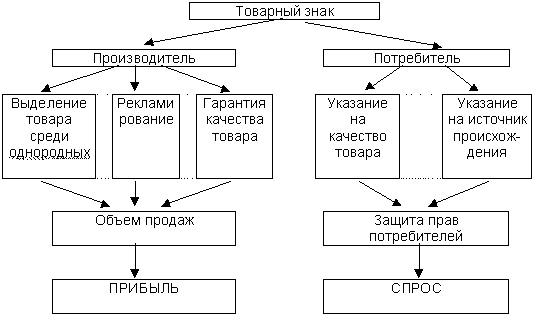
\includegraphics[width=.7\linewidth]{images/pantuhina}
  \caption{Взаимосвязь товарного знака с интересами производителей и потребителей}
  \label{fig:pantuhina}
\end{figure}

  Как видим, основная функция товарного знака -- помочь потребителю выделить
  товар или услуги соответствующего производителя из аналогичных товаров и услуг
  других производителей. Кроме этого, товарный знак дает возможность установить
  источник происхождения товара. Далее, товарный знак, ориентируя потребителя
  при выборе того или иного товара, тем самым становится своего рода гарантией
  качества товара. В этом его вторая функция. Поскольку выбор товара основывается
  на его ожидаемых свойствах, то следующую функцию товарного знака можно обозначить
  как информирование покупателя о наличие того или иного качества в данном товаре.
  Наконец, рекламирование можно также выделить в качестве еще одной функцию
  товарного знака. Иначе говоря, товарные знаки помогают стимулировать и
  сохранять спрос на товары конкретного производителя, тем самым обеспечивая
  широкую известность не только компании производителю, но и товару.

\textbf{Бренд.} Во второй группе это, пожалуй, самый яркий термин,
  сегодня более чем успешно конкурирующий с термином \emph{товарный знак} в
  средствах массовой информации, в публичном дискурсе и повседневном речевом
  общении, как в России, так и за рубежом. Высокая частотность употребления
  того или иного нового слова в практике речи, как известно, фактически
  сводит на нет любые попытки однозначно определить его содержание или значение.
  В переводе с английского <<brand>> обозначает: раскаленное железо, выжженное
  клеймо, фабричное клеймо, фабричная марка, а также выжигать клеймо и
  отпечатываться в памяти, оставлять неизгладимое впечатление\autocite{oxford_dictionary}.
  Исходя из буквального значения этого слова, очевидно, что оно,
  так же, как и \emph{товарный знак}, выполняет функцию индивидуализации товара,
  услуги, или компании производителя, с одной стороны. С другой, такой
  <<индивидуализированный образ>> должен прочно и надолго войти в долговременную
  память потребителя. Понятно, что при этом исполнение самой функции может
  периодически принимать несколько агрессивный характер, опираясь на
  суггестивные возможности знаков коммуникации, о которых мы говорили ранее.
  По факту, бренд, как правило, получает свое материальное воплощение
  в определенном слове, словесном выражении в комплексе со своим
  графическим выражением -- логотипом. В результате, брендом может быть
  наименование товара, услуги, фирмы, не зависимо от того, зарегистрированы
  они или нет. Более того, брендами в последнее время стали называть имена
  ярких исторических личностей, оставивших у нескольких поколений потомков
  неизгладимую память о себе, например: Петр I. Когда в 2002 году британец
  Саймон Анхольт, один из ведущих мировых специалистов в области маркетинга,
  предложил концепцию <<брендинга мест>>, через некоторое время начали
  появляться <<города-бренды>>, <<территории-бренды>>  и
  проч\autocite{brending}. Наконец, судя по последним публикациям по проблеме,
  брендом можно сделать и собственную личность\autocites{peters1999brand}{schawbel2009me}{deckers2012branding}.

  Более детально мы будем говорить о бренде позднее. А пока, в сжатой форме,
  и несколько опережая изложение, сформулируем его суть. Практика показывает,
  что сегодня каждый производитель мечтает превратить свой товарный знак в бренд.
  Очень упрощенно можно предварительно сказать, что термин \emph{бренд} обозначает
  некий
  привлекательный образ, сознательно и изощренно навязываемый  массовому человеку
  извне. В идеале, это образ, непроизвольно возникающий в сознании человека при
  восприятии определенного слова-образа (логотипа), способный формировать мысли,
  образ жизни и поступки человека в массовом обществе потребления. Исходя из
  практики применения этого термина, функцию бренда можно определить как
  формирование автоматических потребительских реакций человека, соматических
  маркеров, при восприятии определенного логотипа.

\textbf{Логотип.} Из сказанного выше, казалось бы, естественным образом вытекает
  представление о логотипе как вспомогательном знаке, графическом атрибутом бренда.


В тоже время, из практики известно, что многочисленные маркетинговые фирмы и
агентства считают логотип  ни больше ни меньше как краеугольным камнем рекламного
бизнеса и по этой причине требующим, помимо всего прочего, весомых финансовых
вливаний. Для примера: британское дизайнерское агентство Marque получило за
разработку логотипа очередных Игр Содружества в Глазго
(XX Commonwealth Games 2014)  \$ 95,000, а логотип для Олимпийских игр прошлого
года в Лондоне принес дизайнерской компании Wolff Ollins  \$ 625,000.
В 2008 году обновление логотипа обошлось компании Pepsi в \$ 1,000.000,
выплаченных дизайнерам фирмы Arnell Group. Логотип корпорации BBC (1997) --
\$ 1,800,000,  логотип консалтинговой компании Accenture (2001) -- \$ 100,000,000,
логотип британской нефтегазовой компании BP (1989) – \$ 210,000,000\autocite{logotipy}.
Каким образом обычный визуальный знак, будучи технически лишь оригинальным
начертанием наименования организации или товара \autocite[][65]{rogers2001marketing},
будучи элементарным средством идентификации -- становится эксклюзивным и
дорогостоящим товаром, мы и попробуем теперь разобраться. Для начала
абстрагируемся от живой социокультурной практики, в которой функционирует
логотип, и посмотрим на знак исключительно в его знаковых характеристиках.
Будем двигаться от общего к частному.

\subsubsection{Знаковые параметры логотипа}
Для удобства сформулируем методологическую матрицу для дальнейшего
рассуждения, обобщив базовые аксиомы знака. Для этого обратимся к
работе А.Ф. Лосева <<Знак. Символ. Миф>> \autocite[][32-42]{losev1982}, где он, в частности,
предлагает различать следующие аксиомы общей информации:

\textbf{Аксиома 1.} \emph{Всякий знак предполагает, что существует нечто внезнаковое
    обозначаемое, и уж тем более нечто означаемое и значащее.} Действительно,
  в конце предыдущего параграфа мы утверждали, что для нас логотип -- знак
  реальный, т.е. если бы для него не было внезнакового объекта обозначения,
  то его нельзя было бы считать знаком. Устранение объекта или произвольный
  выбор объекта означали бы попросту выход из знаковой сферы во внезнаковую
  область.

\textbf{Аксиома 2.} \emph{Всякое обозначаемое и тем более означаемое предполагает,
    что есть знак, которым оно обозначено.} Иными словами, логотип есть не просто
  реальный, но объективно-реальный знак, а не просто абстрактная
  внутрипсихологическая игра понятий.

\textbf{Аксиома 3.} \emph{Всякий знак функционирует как акт обозначения для
    чего-нибудь обозначаемого и уж тем более для всякого означаемого.}
  Проблему с определением внезнакового предмета для логотипа в общем виде
  мы обозначили выше. Данная аксиома просто еще раз утверждает обязательность
  его наличия.

\textbf{Аксиома 4.} \emph{Всякий знак предполагает для себя того или иного
    внезнакового, но вполне специфического носителя.} Логотип, чтобы быть
  самим собой, т.е. иметь свои качества свойства, должен отличаться
  от всего того что им не является. В противном случае мы не могли бы
  говорить о его существовании вообще. Логотип получает свою специфику
  лишь при условии наличия внезнакового носителя, каковым будет
  материал из которого он изготавливается, равно как или материал или
  поверхность на которую он наносится.

\textbf{Аксиома 5.} \emph{Всякое обозначение требует для себя своего
    собственного и специфического, а главное, своего собственного внезнакового
    носителя.} В корпоративной среде конкретным носителем логотипа может быть,
  в частности, внутренняя документация компании, канцтовары,
  наружная реклама, веб-сайт, здание офиса и проч.

\textbf{Аксиома 6.} \emph{Всякий обозначаемый и уже тем самым всякий означаемый
    предмет необходимо требует для себя собственного и специфического, а
    главное, своего собственного внезнакового носителя.}
  Согласно данной аксиоме обозначить нечто -- значит признать, что это
  нечто существует. С другой стороны, обозначить нечто можно только тогда,
  когда это нечто существует. При этом само обозначенное -- в нашем случае
  логотипом -- может быть как глубоким, так и поверхностным, целостным и
  частичным, правильным и неправильным, т.е. может иметь разные способы и
  виды своего обозначения. Наличие общего внезнакового объекта или предмета,
  правильно или неправильно обозначаемого с разных сторон, делает сам
  факт обозначения реально существующим.

\textbf{Аксиома 7.} \emph{Всякий знак предмета есть смысловое отражение
    предмета.} Другими словами, обозначение действительно имеет место
  быть только в том случае, когда знак -- логотип, обозначаемое им и
  сам акт обозначения наполняются определенным смыслом и знак становится
  собственно смысловым знаком.

\textbf{Аксиома 8.} \emph{Соотношение между знаком и обозначаемым, кроме
    их фактического соотношения, находится еще и в состоянии смыслового
    взаимного самоотражения.}

Любой знак есть либо смысл, либо носитель смысла. При этом любое обозначаемое
есть тот предмет, который получил осмысленное содержание при помощи того или
иного осмысленного знака.

От общей аксиоматики перейдем к поиску адекватного осмысленного структурного
определения логотипа. Сначала рассмотрим общепризнанную  классификацию знаков
Ч.~Пирса: иконы, индексы и символы,  основанную на двух дихотомиях --
противопоставлении смежности и сходства, противопоставлении естественной
и произвольной связи\autocite[322]{jakobson1985}. Коротко о каждом.

\emph{Иконическими} знаками называются такие знаки, у которых форма
  и содержание сходны структурно или качественно, т.е. означаемое
  и означаемое фактически подобны. Сам Пирс пишет: <<Иконический знак (icon)
  есть знак, отсылающий к объекту, который он обозначает, просто в силу
  своих свойств, которыми обладает независимо от того, существует ли
  вообще какой-нибудь Объект или нет. Верно, что пока в действительности
  нет такого Объекта, иконический знак не действует как знак.>> \autocite[][185]{jakobson1985}
  Например, рассуждает Пирс, план сражения или батальное полотно есть,
  по сути дела, иконические знаки, если считать их содержанием само сражение.

\emph{Индексом} (index) (или индексальным знаком) называется знак, у которого
  форма и содержание смежны в пространстве или во времени.
  У Пирса мы читаем: <<Индекс есть знак, отсылающий к Объекту, который он
  обозначает в силу того, что он действительно подвергается воздействию
  этого Объекта. (\ldots) Поскольку Индекс подвергается воздействию
  Объекта, он необходимо имеет какое-то общее с этим Объектом Качество,
  и именно в соответствии с ними [качествами] он отсылает к Объекту.>> \autocite[][186]{jakobson1985}
  Например, отпечаток следа на песке, позволяющий сделать предположение о том,
  кто мог пройти в этом месте ранее, вид поднимающегося вверх дыма,
  предполагающий присутствие поблизости огня, ярко выраженные симптомы болезни,
  предполагающие протекание самой болезни, -- все это будут индексальные знаки.
  На самом деле, по-видимому, в данном случае правильнее было бы говорить не
  столько о традиционной смежности формы и содержания, сколько о
  причинно-следственных связях, возникающих между ними.

 Наконец, \emph{символом} (symbol) (или символическим знаком) называется знак,
  для которого связь между формой и содержанием формируется произвольно,
  по некоторому соглашению, касающемуся именно данного знака. В формулировке
  Пирса: <<Символ есть знак, который отсылает к обозначаемому им Объекту в силу
  закона, обычно -- ассоциации общих идей, действующего так, чтобы заставлять
  нас интерпретировать Символ как отсылающий к этому Объекту. Таким образом,
  он сам является общим типом или законом.>> \autocite[][186]{jakobson1985} И если для иконических
  и индексальных знаков форма дает возможность догадаться о содержании знака
  даже не знакомому с ним интерпретатору, то форма символических знаков сама
  по себе, т.е. вне специального договора, не  может дать  вообще никакого
  представления о их содержании.


Следует отметить, тем не менее, что классификация Пирса не носит жесткий,
завершенный характер. Знаки подвижны и могут взаимопроникать друг в друга.
Сам Пирс признает, что, иконический знак может входить в состав индексального
знака, а индексальный знак может быть частью символа, <<хотя это и будет особым
Индексом>>, предупреждает Пирс. Такая подвижность знаков представляется
нам чрезвычайно важной. На самом деле, логотип с легкостью можно было бы
поместить в любую из трех категорий. Во-первых, он является индексальным знаком,
т.е. указывает на конкретного производителя товара или поставщика конкретных
услуг. Он также указывает на конкретную массу потребителей, на которых
ориентирован производимый товар или услуга. Во-вторых, логотип, как
элемент маркетинговой стратегии, может -- и даже должен -- становиться частью
символа, даже амальгама символов и в этом качестве указывать на имидж и
репутацию компании производителя, с одной стороны, и на сложное аффективное
целое позитивных потребительских ожиданий, эмоций и ассоциаций в связи с
деятельностью данного производителя, с другой. В этом случае, в массовом
сознании потребителей он, как <<особый индекс>>, начинает отождествляться
с брендом компании производителя. Наконец, логотип, естественным образом
включает в себя иконическую составляющую. На элементарном техническом уровне,
по форме исполнения, логотип является изображением, иконом, схематически
обобщающий направление деятельности своей компании. На смысловом,
символическом уровне, он лапидарно синтезирует философию компании,
под которой следует понимать ее желаемое представление о себе в сознании
массового потребителя. Иначе говоря, здесь мы имеем дело с функцией двойной
иконической сигнификации. Рассмотрим суть иконичности подробнее.

\subsubsection{Иконичность логотипа}

\paragraph{Философский аспект}

Исторически, идея изобразительной природы знаков, т.е. представление о знаках
как изобразительных подобиях обозначаемых ими объектов, встречается уже в
одном из сократических диалогов Платона, где собеседники делают предположение о
том, что <<имя тоже в некотором роде есть подражание, как и картина>>\autocite{kratil2013}. В
отличие от картины, тем  не менее, знаки здесь понимаются как подражания внутренним свойствам и
качествам вещей. Среди изображений наиболее близки знакам (в узком смысле слова), по-видимому,
рисунки, которые по способу начертания и по своему происхождению родственны знакам письма. Их
родственная связь, в частности, зафиксирована в самой этимологии слова <<знак>>, <<рисунок>>,
<<чертеж>> в разных языках*, утверждая прежде всего их сходство в нанесении каких-то видимых отметок на
плоскости. Примечательно, что родство рисунка с другими знаками может распространяться не только на
видимую форму, но и на невидимое содержание, чему свидетельствуют комментарии мастеров и теоретиков
эпохи Возрождения\autocite[][527-535]{zukarro1981}. Внутренняя форма, или <<внутренний
рисунок>> предмета здесь символизируется, становится идеальным образом первообоазной сущности (идеи),
иначе: божественного первообраза. Например, в английском: <<sign>> и <<design>>, в немецком –
<<Zeichen и Zeichnung>>,  в русском – <<знаменить>>, т.е. наносить рисунок на иконе (однокоренное со
словом <<знамение>>, <<знамя>>, этимологически близкое термину <<знак>> \autocite[][140]{chertov1993}

В крайнем выражении, например, в христианской иконографической традиции
символ и изображение уже полностью отождествляются со своим праобразом,
как подчеркивает, например, П.А.~Флоренский\autocite{florensky1995}.
В результате, постепенно складывается традиция, согласно которой любое
изображение начинает рассматриваться как нечто обладающее большей достоверностью,
чем условный, конвенциональный знак. Более того, изображению начинают
приписывать <<статус документального свидетельства подлинности изображаемого>>\autocite[][143]{chertov1993}. В первую очередь, конечно же, <<иконе>>, появившейся в
христианском искусстве как продолжение давней традиции фиксировать документально
образ умершего \autocite{lihachev1971}.
Парадоксально, но, если иконопочитатели раньше видели в них прямое подтверждение
реальности изображенных объектов культа, то иконоборцы, для которых изображение
как таковое также являлось достоверной копией, напротив,  оспаривали саму
<<возможность документально зафиксировать в иконе вид умопостигаемого божества>>
\autocite[][143]{chertov1993}. Соответственно, для последних изображения на иконах были
всего лишь кощунственными идолами. Компромиссная точка зрения, в конце
концов, восторжествовала: изображение на иконе -- подлинное свидетельство
неизменной внутренней сущности изображаемого, а не случайных внешних
моментов\autocite[][18]{lasarev1986, bichkov1989}.

Должно быть понятно, что большая достоверность изображения по сравнению с
конвенциональным знаком свойственна не только религиозному или
мифологическому сознанию прошлого. Ведь мифологическое сознание в современной
культуре по-прежнему руководствуется теми же самыми представлениями.
Мы как бы <<забываем>> в некоторых случаях, что изображение и изображаемое
совсем не одно и то же. Скажем,
телевизионное изображение того или иного человека рутинно воспринимается
как сам этот человек, а не как знак. Против такого забывания, в
сущности, направлен и интеллектуальный протестный пафос критиков современного
общества потребления, о чем мы говорили ранее. Общества, покупающего себе образы
(shopping for images)\autocite{ginsberg1984supermarket}. Для нас же здесь вопрос о
достоверности конвенциональных знаков и изображений лежит в плоскости аналогии.
Ошибочные, ложные или просто фантастические представления, как мы знаем по
рекламе, могут в равной степени легко передаваться как знаками, так и
изображениями. Скажем, сам факт изображения Снегурочки вряд ли покажется
достаточным основанием для признания ее реальности. Как знаки, так и
изображения -- это средства коммуникации, и как таковые они способны в равной
степени передавать достоверные и недостоверные сведения. Именно на основании
общности коммуникативных и репрезентативных функций изображений и условных знаков
Ч.~Пирс включает изображения в  свой знаковый триптих.

Все это пока лишь самое общее обсуждение иконичности, имеющее отношение
к логотипу лишь постольку, поскольку в плане выражения он  является иконическим
знаком и, в свете сказанного выше, также может получать двойственное
истолкование. Однако поменяем  фокус анализа.

\paragraph{Психологический аспект}

В посмертно опубликованной работе
<<Экзистенциальные графы>> Пирс также пишет: <<Бытие иконического знака принадлежит
прошлому опыту. Он существует только как образ в памяти>>.
(Цит.~по:~\autocite{jakobson1983}) То есть речь идет о припоминании или
узнавании общих качеств и свойств узнаваемого объекта. Но именно эту общность
свойств и качеств знака и объекта ставит под сомнение У.~Эко, для которого
отношение иконического знака к реальному объекту лежит за пределами собственно
семиотических отношений. По его представлению иконический знак также условен,
как и конвенциональный знак. Подобно <<автоматизированному рефлексу>>  он
воспроизводит лишь некоторые общие условия восприятия объекта, и их сходство
определяется ментальной репрезентацией, перцептивной моделью, вызываемой
объектом в психике субъекта. В знаке отображается не то, что видит художник,
а только то, что он знает о видимых, предполагаемых и конвенциональных свойствах
и качествах предмета. <<Иконические знаки, -- считает Эко -- воспроизводят
некоторые условия восприятия объекта, но после отбора, осуществленного на
основе кода узнавания, и согласования их с имеющим репертуаром графических
конвенций>>\autocite[][160]{eko1998} Иначе говоря, для распознания
изображения мы используем данные о знакомых, виденных вещах и явлениях, которые
хранятся в долговременной памяти в качестве неких эталонов.  Как и в случае с
восприятием речи, распознавание изображения делается возможным благодаря коду
узнавания, который вычленяет отдельные существенные черты предмета для хранения
в памяти и дальнейшего использования в коммуникации. Так, например, мы можем
издалека распознать зебру и даже воспроизвести ее на рисунке, опираясь лишь на
две наиболее существенные черты: полосатость и четвероногость, абстрагируясь от
остальных подробностей ее анатомии. Причем функционирование кодов узнавания
(как и кодов восприятия), полагает У.~Эко, в значительной степени детерминировано
культурным фоном, или точнее -- конвенцией визуальной репрезентации в различных
культурах. Если для нашего культурного мировидения  зебра экзотична и необычна
по сочетаемости полосатости и четвероногости, то, скажем, для кенийского
африканского племени, промышляющего охотой на зебр, значимыми могут оказаться
совершенно иные свойства\autocite[][160]{eko1998}.

Примечательно, что семиотические интуиции У.~Эко, с одной стороны, перекликаются
с отечественной психологической теорией знака, о которой мы говорили ранее,
с другой,  находят свое подтверждение в том числе и в результатах современных
нейро-исследований физиологии зрительного восприятия человека. Исследователи,
в частности, утверждают, что представление о наличии оптического образа,
передаваемого глазного яблока на экран -- зрительную кору головного мозга --
очевидное логическое заблуждение. Для нейрофизиолога человек -- в высшей степени
визуальное существо, в том смысле, что у него в задней части головного
мозга функционируют тридцать зрительных полей, позволяющих ему видеть мир.
Каждая из этих зон, как показывают исследования, вероятно отвечает за разные
аспекты зрения\autocite{velyanur2006}.

Поэтому для понимания зрительного восприятия необходимо <<забыть про идею образа
в мозгу, а вместо этого подумать о преобразовании или символическом
представлении объектов и событий во внешнем мире.>> \autocite[][33-34]{velyanur2006}
Точно также как знаки письменности представляют или символизируют нечто,
чем они не являются физически, так и воспринимаемые нами события и предметы
внешнего мира являются результатом активности нервных клеток мозга и
разнообразных примеров их работы. При такой постановке вопроса нейрофизиологи
становятся своего рода дешифровщиками, пытающимися <<взломать чужой код>>,
т.е. <<код, который использует нервная система для изображения внешнего мира.>>\autocite[][34]{velyanur2006}.
Иными словами, нейрофизиологи тоже становятся семиотиками.

Два важных следствия для понимания иконичности логотипа:
\begin{enumerate}
\item Его изобразительность есть отражение лабильности внутренней
  психической жизни (деятельности мозга) дизайнера -- его создателя, в одном
  случае, и воспринимающего (смотрящего на него) реципиента, в другом.
\item В обоих случаях восприятие апперцептивно и обусловлено культурным
  контекстом, в широком смысле слова.
\end{enumerate}

\paragraph{Прагматические аспекты логотипа}

Новый прагматический подход к описанию знаков и знаковых систем предложил
современный израильский филолог и семиотик А.Б.~Соломоник\autocites{solomonik1995}{solomonik2004}{solomonik2009}.
В частности, он предложил классифицировать знаковые системы по принципу
эволюционного развития и на основе образующего их базисного знака.
Все существующие знаковые системы иерархически распределились по пяти типам и
по пяти видам знаков с нарастающей степенью абстрактности: естественный знак,
образ (имидж), слово, иероглиф, символ с постоянным значением, символ с
переменным значением\autocite[][76-86]{solomonik2009}. Так как мы не имеем
никакой возможности рассмотреть здесь все классификацию целиком, мы
ограничимся лишь обозначением направления классифицирующей мысли автора
концепции и кратким описанием  базовых знаков трех первых уровней.

Естественные знаки -- осязаемые предметы или явления природного происхождения,
представляющие другой предмет или явление. Так, следуя логике <<если \ldots, то \ldots>>,
по лужам мы можем судить о прошедшем дожде, по свету от лампы о том,
что нужный нам человек возможно еще не спит и т.д. Соломоник называет их
<<первыми в истории знакового взаимодействия между природой и человеком>>\autocite[][78]{solomonik2009}.
Над ними надстраиваются уже знаки, придуманные человеком, и в первую очередь --
образы. Точно так же как образное мышление приходит сразу вслед за
манипулированием предметами в развитии маленьких детей и перед стадией
овладения языком, образ как базовый знак нового уровня надстраивается над
естественным знаком и его системами, взаимодействуя с ними, вбирая и представляя
их по-новому. Знак-образ уже не является реальным предметом. Это изображение
чего-то из реальности, связанного с ним отношением, близким к изоморфизму,
т.е. по наличию точек совпадения по конструкции и/ли по содержательным
компонентам. Совпадения <<либо по существу, либо по внешнему виду, либо по
ассоциациям, вызываемым образом и изображаемым>>\autocite[][52]{solomonik1995}.
Этот тип, соответственно, включает в себя очень большое количество
знаковых систем -- ориентировочных, рисуночных, игровых и проч.
Наконец, следующая стадия в развитии человека (и человечества),
приходящая после овладения началами образного представления -- шифрование
окружающей реальности при помощи слов языка. Слова уже существенно абстрактнее
знаков-образов по причине значительной произвольности и удаленности от
своего референта.

Остановимся здесь. Пожалуй, главное в систематизирующей мысли А.Б. Соломоника:
<<каждый переход от одного базисного знака к другому сопровождается изменением
объема шифрующейся в одном знаке действительности>>\autocite[][79]{solomonik2009}.
Естественный знак шифрует данный предмет в каждом конкретном случае, образ
уже начинает стремиться к родовому обобщению, в то время как основная
масса слов -- это коллективные понятия. Посмотрим более внимательно на категорию
знака-образа, своего рода прагматическую альтернативу икону Ч.~Пирса.

Любой знак-образ изначально материализуется в виде реальных предметов.
Если положить часы в витрину магазина, то это будет естественный знак того,
что здесь продаются часы. В то же время нахождение часов в витрине делает
этот знак в некотором степени образным, поскольку они представляют не только
те конкретные часы, которые продаются в данный момент, но продажу часов вообще.
То есть знак-образ призван представлять все аналогичные предметы данной группы.
Нарисованные часы на витрине магазине становятся знаком в полном смысле слова,
хотя только знаком-образом. Если же на вывеске магазина написать <<Часы>>,
то это будет знаком языкового кода, который, по сути дела, будет выполнять
ту же самую функцию, что и нарисованные часы, равно как и настоящие часы в
витрине. А если к яркому изображению на вывеске магазина добавить логотип
знаменитой часовой компании, то образ сразу же приобретает символический
характер, свойственным формализованным символическим системам в классификации
А.Б.~Соломоника.

Одни знаки-образы в большей или меньшей степени внешне похожи на реальный референт.
В этом случае речь идет о знаках-<<иконах>>, распространенных в практической жизни
гораздо больше остальных знаков <<просто потому, что вследствие своей похожести на
изображаемое они понятны всем категориям пользователей и не умеющим читать и даже
не знающим языка страны, где они находятся.>> \autocite[][55]{solomonik1995}
Так, рисунок ботинок на вывеске достаточно ясно указывает на магазин обуви или мастерскую по
ремонту обуви. Понятно, что чем популярнее изображаемый объект в мире -- скажем,
продукты питания -- тем быстрее распознается изображение. В других случаях культурная
традиция данного общества и даже местные обычаи ограничивают понятность даже
самых отчетливых <<икон>>. Более того, иногда -- даже в пределах одной страны -- для
одного изображаемого могут использоваться разные <<иконы>>. Варьирование достигается
преимущественно за счет использования разных тропов -- часто метонимии и синекдохи --
для построения образа. Например, нарисованный конверт -- простой пример знака, обозначающего почту.
К универсальным системам, построенным преимущественно на иконах, относится система
дорожных знаков \autocite[][56-58]{solomonik1995}. Логика такой системы достаточно
примитивна, поскольку каждый знак в ней оценивается по отдельности и в каждой
конкретной ситуации.

Другие знаки-образы ковенциональны, т.е. исключительно условны и произвольны
по обозначению вложенных в них идей сходства между изображаемым и его символикой.

Например, на гербе Российской Федерации изображен двуглавый орел,
отражающий силу и мощь государства, символ союза светской верховной власти  и власти духовной.
Изоморфизм здесь, казалось бы, практически равен нулю. Но только по
схожести внешних признаков. Иначе говоря, он уступает место внутреннему изоморфизму:
<<по связи образа с изображаемым через представляемые или культурно-обусловленные
символы>> \autocite[][61]{solomonik1995}. В исторической перспективе, по мере
усложнения форм социокультурной практики жизни, человеку уже недостаточно просто
регистрировать происходящее и знаки-образы получают дополнительную смысловую нагрузку,
чтобы передавать сложные внутренние связи между предметами и свое отношение к изображаемому.
Реалистичный знак-образ начинает все больше тяготеть к синтетическому визуальному обобщению
и новому статусу образа-символа. Соответственно, нарастает и степень его абстрактности.
Чем выше степень абстрактности знака и чем слабее его связь с обозначаемым
референтом, тем легче оперировать им внутри знаковой системы: образовывать
сложные знаки из базисных, составлять сложные выражения из простых знаков, давая
им большую степень свободы и новые эвристические возможности и качества.
И последнее: получающийся сложный образ, как,  впрочем,  и образ вообще, невозможно
разложить на простые составляющие компоненты, что, в свою очередь, <<не дает нам
возможности подключить при восприятии разум; мы вынуждены реагировать
эмоционально>>\autocite[][77]{solomonik1995}.

Думается, подход А.Б.~Соломоника имеет несколько преимуществ перед трехчленной
схемой Ч.~Пирса. Во-первых, здесь распределение знаков происходит по
иерархическому принципу, последовательно и в нарастающем порядке. Во-вторых,
в основу классификации положен единый критерий степени абстракции знаков,
позволяющий наглядно представить динамику постепенного отдаления знака от
своего референта и обретения им расширяющихся синтаксических возможностей в ту
систему, куда он включается. В-третьих, каждый вышестоящий знак в иерархии
приобретает дополнительные возможности охватывать все большие сегменты реальности,
которые он шифрует.

Соответственно, в этом плоскости рассуждения логотип у нас переходит из категории
индексов Пирса, которым при данном подходе соответствуют естественные знаки,
в категорию знаков-образов, первых собственно знаков с потенцией обобщения и
интериоризации опыта. Из двух описанных выше потенций быть  образом-иконом
или конвенциональным образом-символом, мы определяем логотип в категорию
образов-символов. В следующем пункте мы поместим логотип в социокультурный
контекст и рассмотрим предпосылки и генезис его символической эволюции.
Но сначала обобщим сказанное:
\begin{enumerate}
\item По функциональному назначению логотип есть коммерческий знак-образ.
\item По своей способности обобщения логотип есть эвристический знак-символ.
\item По своей способности отражения сегментов реальности логотип конвенционален и условен.
\item По факту психического отражения логотип воспроизводит соотношения схемы
  взаимодействия перцептивных и апперцептивных факторов в сознании дизайнера-изготовителя
  и реципиента-потребителя.
\end{enumerate}

\paragraph{Символичность логотипа}
По словам П.А.~Флоренского: <<Основание символики -- самая
реальность>>\autocite[425]{book:florensky1}. В повседневном речевом общении и прикладной
деятельности под символом (от греч. <<знак, опознавательная примета>>) обычно
понимается графическое изображение знака, буквы, предмета, действия или явления.
В философии и гуманитарных науках символ это любой предмет или явление,
пластический или словесный образ, который какой-то смысл, т.е. личностную ценность,
как мы подчеркивали раньше. Понимаемый таким образом символ указывает на значимость,
ценность данных предметов, явлений и проч. как для отдельной личности
(индивидуальные личностные символы), так и для малых и больших, массовых групп,
в том числе народов, государства, человечества в целом. Так, голубь и изображения
голубя могут восприниматься как мировой символ ценности, значимый для всего
человечества.

Символическая ценность логотипа, разумеется, не имеет масштабов общечеловеческой ценности.
В то же время его массовое присутствие в повседневной практике жизни в современном
обществе позволяет назвать его феноменом поистине мирового масштаба. Реальность
бытия логотипа, в которой раскрываются его символические качества -- как в его графическом
воплощении, так и в его идейности - образует своеобразный континуум.
Крайние полюса этого континуума оформляет один и тот же детерминант -- бренд.

\paragraph{Социокультурный генезис логотипа}

В самом начале параграфа мы говорили, что логотип решает задачи закрепления права
собственности, идентификации и выражения социального статуса обладателя.
Последовательно расширим этот тезис.

% Логотип и его эквиваленты, согласно профессиональной литературе по графическому
дизайну и маркетингу, ровесники самой человеческой цивилизации. Так, первым логотипом,
в исторической перспективе, принято считать бренд-клеймо (древ. сканд. \emph{brandr},
<<гореть>>, анг. \emph{brand} -- <<отпечаток>>)\autocites{markritson}{colapinto2011}{tradetimeline}{zapenko2007}.
Изначально нанесение клейма -- или брендинг -- предполагало прижигание плоти
каленым железом с целью получения отпечатка с легко узнаваемой конфигурацией,
который должен был выполнять функцию идентификатора и знака владельца.

Были времена, когда подобные физические клейма принудительно ставили на людей --
на мужчин и женщин одного рода или племени, на рабов и крепостных крестьян;
как форму наказания -- на воров, дезертиров и уголовных преступников и т.д.
Известно, например, что практику наказания брендом применяли древние греки и
римляне, а позже ее переняли англосаксы, и популярность ее постепенно сошла на
нет в Англии примерно к середине 19 века. Сейчас практика грубого клеймления ограничена
клеймлением скота, которая, думается, также является поучительной  частью общей традиции.

Так, известно, что брендинг крупного рогатого скота и лошадей проводился в древнем
Египте уже 2,000 лет до нашей эры. В Северную Америку брендинг прибыл вместе с
конкистадорами Х. Кортеса в 16 веке и распространился первоначально в Мексике,
а затем был позаимствован техасскими скотоводами как средство защиты от воров.
Отпечаток часто принимал форму изощренного тавра -- комбинации фигур, букв и символов,
которые трудно было изменить и, соответственно, присвоить чужую собственность.
В США брендинг скота сегодня проводится не столько в целях свидетельства права
собственности, сколько для учета его родовых племенных качеств. В большинстве
скотоводческих штатов официальная регистрация бренда-тавра предусмотрена
законодательством, а его самовольное изменение квалифицируется как уголовное
преступление\autocite{1994encarta}.

Одним из парадоксов сегодняшних дней, однако, является известный феномен
добровольного физического брендирования, предлагаемого, в частности, в виде
услуг тату-салонов. За умеренную плату можно сделать себе татуировку любой
конфигурации и размеров, с использованием безболезненных химических реагентов
и новых электронных технологий\footnote{см., например, \autocites{digitaltattoo}{tedtattoo}}
Речь здесь, по всей видимости, уже следует вести о маркерах визуальной
самоидентификации и саморекламе, когда в знаке приглушается овеществляющая
составляющая его денотативного значения и доминантным становится его символический
коннотат. Но физический брендинг, естественно, является всего лишь самой примитивной
архаичной формой наращивания символической функции изображения. По-настоящему
полное выражение символизм логотипа получил благодаря постоянному улучшению
орудий труда и технологий в
\begin{enumerate*}[label=\asbuk*)]
    \item ремесленно-промышленной и художественно-эстетической деятельности человека-производителя;
    \item сакрализации этикета, ритуалов, знаков величия и статуса правящей элитой в
    классовом обществе.
\end{enumerate*}
Именно в этой бурной стихии практической жизни получает свое полное
развитие символический брендинг.

%% TODO: источник!
В области экономической деятельности, индивидуальная маркировка изделий мастерами
ремесленниками, первые водяные знаки на бумаге (13 в.), штампы для бескрасочного
тиснения, торговые отметки и штампы на ювелирных изделиях и т.д. -- все это примеры
ранних логотипов. Тем не менее, следует признать, что по-настоящему массовая маркировка
продукции началась в период индустриальной революции с возникновением массового производства,
массового рынка и появлением фасованных товаров массового потребления и упаковки.
Индустриализация перенесла производство многих предметов домашнего обихода от
мелких местных производителей на крупные централизованные заводы. При перевозке
товара заводы в 19 веке в обязательном порядке наносили свой логотип или надпись на
свою тару или упаковку, тем самым, фактически,  отождествляя понятие <<бренд>>
с  товарный знаком-логотипом.  Знак производителя на упаковке помогал отличать
товары, привезенные с крупного завода, от продукции местных производителей конкурентов.
Более того, необходимо было также убедить потребителя, что новым неместным товарам
можно доверять в равной степени, как  и товарам местного производства. Так, для
американской компании, производившей сухие завтраки Kellog’s  роль различительного
знака выполняла подпись основателя компании\autocite[][8]{evami2009}. Другие компании использовали
для этой цели персонифицированные образы. Например, розовощекого квакера (Quaker Oats),
чернокожего Дядюшки Бена (Uncle Ben, выращивающий рис в Техасе) или
Тетушки Джемаймы (Aunt Jemimа, пекущая блины для своего белого хозяина и его гостей) \autocite[][8]{evami2009}.
Так начинался процесс воспитания массового потребителя.

В первой половине 20 века компании-производители начали придумывать остроумные
рекламные слоганы, яркие маскоты, и  джинглы, регулярно появляющиеся на радио и
раннем телевидении. А к 1940-м годам производители вместе с тем начали проявлять
все больший интерес к практическим научным исследованиям культурных,
социально-психологических, личностных особенностей и потребительских привычек массового
покупателя. Что они собой представляют, как они формируются, и главное -- как на них можно
влиять \autocite{kotlergrayson}.

Массовый выпуск товаров и ожесточающаяся конкуренция на рынке стимулировала поиск
новых оригинальных эвристических идей и стратегий сбыта товаров. <<Бренд>> -- на
этот раз переосмысленный как концепция или философия ведения бизнеса –- по
принципу метонимического переноса сместил смысловой акцент в знаке с расхваливания
предполагаемых достоинств производимого товара на предполагаемые достоинства самого
производителя, на его пусть символическую, но крайне привлекательную  идентичность-бренд.
Тщательно продуманный символический брендинг сегодня подразумевает уже не только
наличие идентифицирующего <<отпечатка>> на самом товаре, но и обязательное наличие
его в сознании массового потребителя в виде эмоционально заряженной позитивной
ассоциативной памяти. Такой потребитель покупает уже не столько конкретный товар,
сколько его <<бренд>> -- о чем писали Ж.~Бодрияр, М.~Фуко, Р.~Барт, Г.~Маркузе, Э.~Фромм
и прочие критики общества потребления. Он брендирован. То есть становится хотя и
символической, но стабильно приносящей прибыль собственностью компании, ее активом.
Но это только одна сторона вопроса. <<Отпечаток>> в памяти, как показывают
современные нейрофизиологические исследования, есть не только эгоистичный вирус
потребления, инфицирующий сознание потребителя извне, но, что важнее, еще и желаемый
мем-accоциация, структурный элемент его
Я-концепции\autocite{browdy2006}\autocite{mesheryakov2004}.

Мартин Линдстром -- на сегодняшний день один из самых именитых специалистов в
области нейро-маркетинга и рекламы -- осторожно сравнивает отношение массового
потребителя к любимым брендам с религиозным чувством, подразумевая, что брендинг
и религия задействуют общие психологические механизмы массообразования. Например,
в одном месте он популярно обобщает: <<Несмотря на различия, основные мировые
религии зиждутся на десяти столпах: общности верующих людей, ясном видении
своего предназначения, чувстве превосходства над противниками веры,
чувственном восприятии мира, сакральных текстах, прославлении своего величия,
проповедовании ``Святого Писания'', символизме, чудесах и религиозных обрядах>>\autocite{lindstrom2010}
Далее, Линдстром последовательно и подробно излагает результаты своего исследования,
сравнивая воздействие логотипа-марки-бренда с воздействием религиозных ритулов,
обрядов и символов. Касательно символов эксперимент показал: <<Реакция мозга
участников эксперимента на бренды и религиозные символы была не просто похожей,
но одинаковой>>\autocite{lindstrom2010}. По ходу изложения он также дает
многочисленные примеры того, как маркетинговые фирмы, рекламные агентства
и отдельные компании производители сегодня активно берут на вооружение технологии массобразования,
заимствованные у института церкви и как осознанно формируется эмоциональная и
психологическая зависимость массового потребителя от визуального присутствия и
потребления брендов в повседневной жизни.

Можно различать два этапа возникновения и культивирования зависимости от логотипов-марок.
На первом этапе, называемом в маркетинге, <<стадия рутины>>, мы как потребители просто
используем некоторые торговые марки или товары как  повседневную привычку и ритуал:
чистим зубы пастой Blend-A-Med, моем руки мылом Safeguard и т.д. Все эти товары мы
регулярно покупаем и заменяем или восполняем, когда они заканчиваются или ломаются.
На втором этапе, именуемом <<стадия мечты>>, -- обычно на отдыхе, на выходных, в отпуске,
когда нас застали врасплох, т.е. во время наибольшей предрасположенности к
суггестивному воздействию, мы покупаем вещи -- новую одежду, новые аксессуары --
<<не потому, что мы в них нуждаемся, а потому, что позволили эмоциональным сигналам
об этих продуктах проникнуть в наш мозг>>\autocite{lindstrom2011brandwashed}.
Принцип прост: на отдыхе мы чувствуем себя более свободными, более открытыми для
новых ощущений, новых предметов гардероба, новой косметики, новой еды и т.д.
Но очень скоро приятные воспоминания или позитивные эмоции <<этапа мечты>>
начинают неосознанно связываться со вкусом нового блюда или с впечатлением
от нового гаджета, или с запахом новой туалетной воды. Разумеется, в будущем мы
постараемся <<восстановить>>  приятное радостное ощущение, и, помимо всего прочего,
включить новые логотипы-марки-бренды и товары в свою повседневную жизнь,
сделать их привычной частью своего мира. Затем цикл повторяется.

Таким образом, мы представили символическую эволюцию логотипа как движение
от акта физического обезображивания к современному символическому брендингу по
признаку обозначения  права собственности (владения) и идентификации. В этом отношении,
несмотря на очевидные внешние формальные различия, думается, суть нанесения метки-знака
на животное, товар или человека не претерпело существенных изменений. В то же время,
следует отметить радикальное изменение полярности в оценочной части значения знака,
с точки зрения статусных ожиданий. Если раньше хозяйственное и уголовное бренд-клеймо
попросту нивелировало статус человека, превращая его вещь или изгоя общества, то
современный бренд-марка, во всяком случае, в публичном дискурсе, помещает его
на самый верх статусной иерархии массового общества.  Другими словами, логотип
(бренд, марка) выполняет функцию тройного обозначения, а именно: товара,
производителя, потребителя. При этом важно понимать, что потребитель совсем
не обязательно всегда является пассивной жертвой коварных знаково-символических
манипуляций крупных корпораций. Можно представить сложившееся положение дел и
по-другому: массовый потребитель, в поисках своей идентичности, в соревновании за
статус и самоутверждение сам помогает бизнесу принимать стратегические решения и
эффективно адаптироваться к запросам рынка, каковым и является массовое общество потребления.

И здесь мы снова поменяем угол рассмотрения проблемы. Перейдем из области товарно-денежных
отношений в социальную среду и посмотрим на логотип  теперь уже вне связи с брендом или
товарным знаком. Ведь логотип -- это тоже <<отпечаток>>
(др.-греч. <<\foreignlanguage{greek}{λόγος}>> -- слово
и <<\foreignlanguage{greek}{τύπος}>> -- отпечаток.) Отпечаток логоса в сознании, его эмблема.

\paragraph{Эмблематические  истоки логотипа}
В типографике начала XIX века термин <<логотип>> использовался в качестве синонима
другого термина -- <<лигатура>> для обозначения объединения двух или трёх знаков
типографского шрифта. В XX веке логотипом уже стали называть стилизованное
шрифтовое и графическое начертание названия коммерческой организации или товара
(его торговую марку) или само название в таком начертании \autocite[][50]{lebedev2013logos}.
Автором термина <<логотип>> является граф Чарльз Стэнап, единственный пэр Англии
конца 18 -- начала 19 вв., вошедший в историю как талантливый ученый, инженер и
изобретатель \autocite[][50]{lebedev2013logos}. В 1800 г. Стэнап изобрел печатный пресс с ручной
подачей бумаги и технология логотипа. Томас К.~Хансард в своем труде <<Типография:
исторический очерк возникновения и становления искусства печати>> (1825) приводит слова
самого Стэнапа: <<Я посчитал целесообразным создать новую пару составляющих наборной
кассы (\ldots) ввел новый набор двойных букв (это: on, of, to, re, an, th, in, se; они
не печатались в виде лигатур) которые я называю логотипами; и отказался от двойных
букв {ff}, {fi}, {fl}, {ffi}, {ffl}, {ft}, которые ранее занимали место в наборной кассе,
но использовались так редко (\ldots)>>\autocite{logotype}.


Итак,  первые логотипы в истории культуры: on, of, to, re, an, th, in, se.
Сейчас уже не представляется возможным доподлинно установить, почему именно граф решил назвать
эти буквосочетания новым именем, а не причислил их к классу обычных лигатур.
Общее прототипическое значение лигатуры -- нечто, служащее для объединения, соединения.
Лигатура есть знак любой системы письма или фонетической транскрипции, образованный
путём соединения двух и более графем. Можно предположить, однако, что при отборе
восьми буквенных сращений Стэнап руководствовался не только, и не сколько практическими
соображениями технически ускорить процесс набора текста. С одной стороны, данные
сочетания, по всей видимости, действительно имеют высокую частоту встречаемости
в письменной речи. С другой стороны, в силу своей частотности они в определенном
смысле включают в себя внутреннюю энергию бурной стихии самого языка, в той мере,
в какой она запечатлена в уникальной технологии фонетического алфавита. Для примера,
М.~Маклюэн решительно настаивает на том, что фонетически записанное слово есть
результат внезапного разрыва между слуховым и визуальным опытом человека, а
сам фонетический алфавит является ни больше, ни меньше -- грандиозной технологией омассвления
и единообразия,  создающей для всех культурных институтов общий метод трансформации и контроля.

Более образно о том же в автобиографии африканца Принца Модупе <<Я был дикарем>> (1958):
<<Постепенно я начал понимать, что значки на страницах -- это пойманные в капканы слова.
Каждый мог научиться расшифровывать эти символы и, освобождая пойманные слова из капканов,
снова превращать их в речь. Типографские чернила залавливали мысли в ловушки;
теперь те могли вырваться на свободу не более, чем думбу из западни>>\autocite[][92]{macluan2011}.
%% TODO: библиографическая ссылка.

Таким образом, перед нами самобытное определение письменного знака,
<<залавливающего мысли в ловушки>>. Надо полагать, что освободиться из такой
ловушки непросто не только курдючной овце, но и человеку без специальной подготовки.
Вместе с тем, и логотип, в дополнение ко всему тому, что уже было сказано о нем,
также является письменным знаком, и, следуя предложенной логике, также залавливает
мысли в ловушки единообразия и стандартизации, типизирует Логос\autocite[][50-52]{lebedev2013logos}.
% TODO: wat?
Скажем иначе: логотип не просто обладает потенцией символизации в той мере,
в какой это присуще конвенциональному знаку-образу. (см.~\ref{3.3.3}) Это верно,
но лишь в определенных пределах. Сочетание элементов словесности и
изобразительности, с одной стороны, ставит их в отношения взаимной дополнительности
по типу классической эмблемы. С другой, помещает его в разряд символических
вторичных систем записи, ориентированных в первую очередь на передачу сообщения,
а не на фиксацию его на длительный срок\autocites[][190-198]{solomonik1995}[][70-73]{solomonik2009}.

У представленного таким образом логотипа появляется новая генеалогическая
родословная по линии развития систем письменности и соответствующем усилении
степени абстрактности знака. Так, предтечами и зачастую образующими элементами
стиля современного логотипа становятся пиктограммы, иероглифы, родовые рыцарские
гербы, эмблемы и проч. В то время как сам логотип становится особым условным обозначением --
абстрактным символом. Особый интерес для нас в этом перечне представляет эмблема.
Прежде всего тем, что эмблема представляет собой точно фиксированный,
конвенциональный знак. А также тем, что, несмотря на это, эмблема, по причине своего
достаточно широкого функционирования, одновременно может быть и символом\autocite[][268]{losev1976}.
В более узком прагматическом смысле, эмблема интересна нам, во-первых,
своим формальным сходством с логотипом по сочетаемости графического изображения и слова.
Во-вторых, своей способностью символизировать <<коллективную принадлежность и цель>>\autocite[][14]{elbrunn2003}.
В-третьих, своей социальной ориентированностью на быструю идентификацию особого статуса обладателя.

Известно, что геральдическая эмблема появляются в средневековой Европе во время
расцвета феодальных отношений. Геральдические опознавательные знаки в целом, и
эмблема в частности, помогали классифицировать людей по социальным группам в
общей структуре феодального общества. Не будучи официально выстроены в легальную
систему, эмблемы (гербы), тем не менее, в течение многих веков предназначались для
самоидентификации знатных рыцарских родов и кланов. По выражению Ю.М.~Лотмана, в
определенных культурно-семиотических ситуациях вещь тяготеет стать словом и
обрастает знаковыми признаками, становясь эмблемой\autocite[][341-342]{lotman2002}.
Аксессуары средневекового высшего общества становились неизбежно такими говорящими эмблемами.
Подобно современному логотипу эмблема, помимо простой орнаментальной функции,
в то время представляла собой знак самоидентификации особой знатной личности или
группы. В тоже время, она представляла собой знак имущей власти и особого
статуса в социальной иерархии. По мере разрушения духовной вертикали как основы
понимания мироустройства и утверждения более светского восприятия жизни в середине
XIX века, символическая валентность эмблем самим себе утрачивает свою актуальность.
Но уже на рубеже веков эмблемы, образы, слова, предметы <<обретают символическую
нагрузку через сознательную текстуальную стратегию>>\autocite{rebekkini2006}.

К одной из таких стратегий в современной массовой культуре и  в ностальгическом маркетинге,
по-видимому, следует отнести  медиевизм, увлечение
Средневековьем\autocites{eco1986dreaming}{eco1986living}{lindstrom2011brandwashed}.
Как правило, такой медиевизм принимает форму эскейпизма в воображаемый
героический и романтический мир средневековой рыцарской символики, рыцарства и
его атрибутов. При этом средневековые геральдические знаки самоидентификации эмблемы
(гербы) естественным образом наполняются современным содержанием,
подчеркивающим особый статус и престиж человека, обладающего
ими\autocites{elistratov2004}{bergelson2002}.
Более того, психологически они также активно влияют на построение Я-концепции
(self-concept) такого человека, на его представления о самом себе, особенно
в той части, где они опираются на оценку и одобрение других людей (public self-image)\autocite{mesheryakov2004}.

%% TODO: какая ссылка правильная? 1.3 у нас нет.
Об эмоциональной потребности человека ощущать свою сопричастность какой-то массовой
общности мы говорили в \ref{1.3}. К сказанному теперь можно добавить потребность в ощущении позитивной
обратной связи: <<потребность в том, чтобы быть принятым другими и даже нравиться им; чтобы к тебе  относились как полноправному члену группы; чтобы знать, что твои желания разделяются остальными>\autocite{yule1996pragmatics}. Другими словами, потребность в приобретении
подобаемого социального статуса, самоидентификации в престижном качестве.

В отличие от прошлых эпох, когда статус мог присваиваться по факту происхождения,
по предписанию или за особые заслуги перед правящим монархом, в массовом обществе
потребления социальный престиж переосмысливается в терминах финансового успеха и
демонстративного, показного потребления. Соответственно, престижный социальный статус
в таком обществе в буквальном смысле приобретается в конкурентной борьбе потребителей,
соревнующихся в утверждении превосходства своих вкусовых предпочтений в выборе товаров.
Массовое страстное проявление лояльности и верности тому или иному товару или компании
производителю сегодня получило ироническое название
<<fanboyism>>\autocite{mcraney2011you}.
Он работает по принципу: чем выше стоимость покупки, тем интенсивнее рационализация
ее достоинств потребителем. Чем убедительнее его придуманный нарратив, оправдывающий
целесообразность и преимущества приобретенного товара, тем заразительнее
суггестивный эффект, который он производит на других потребителей. Наконец, тем
\begin{enumerate*}[label=\asbuk*)]
\item быстрее образуется и разрастается потребительская массовая общность,
\item быстрее растет самооценка и ощущение значительности ее членов,
\item быстрее растут продажи данного товара,
\item выше поднимается статус компании в глазах потребителей.
\end{enumerate*}
Цепочка замыкается. Производитель получает желанную прибыль, потребитель --
желанный товар и желанный престиж, а современная потребительская концепция счастья --
свое материальное выражение \autocite[][15-23]{lebedev2012}. Однако, снова вернемся к эмблеме и логотипу и их
роли в этом процессе.
%% TODO: ссылка на статью

\begin{enumerate}
\item На самом элементарном уровне эмблема, также как и логотип в
  своей базовой функции, обеспечивают моментальное узнавание. Различие
  между ними как маркерами статуса сегодня, по-видимому, главным образом
  есть вопрос вкусовых предпочтений. Оба опознавательных знака представляют
  собой изображение с фиксированным, однозначным смыслом, который можно представить
  как визуальное воплощение имиджа компании. Имидж компании  в коммерческой
  деятельности -- это специально создаваемый образ-представление, построение
  которого требует определенного упрощения, преувеличения и стилизации основных
  черт реального предприятия или фирмы, которые затем отображаются в знаке-идентификаторе.
  Стилизованное, упрощенное и преувеличенное изображение в знаке, как правило, получает
  акцент на каком-то одном доминантном отличительным признаке компании, что, собственно,
  и делает возможным его моментальное узнавание в ряду других, похожих опознавательных
  знаков\autocites{raigorodski2001}{melnik2001}[][88-99]{karasik2011}. Все это должно быть самоочевидно.
\item В то же время, как мы неоднократно отмечали выше, изолированный знак, с
  однозначной функцией, в сущности, представляет собой самую примитивную форму знака,
  как, например естественные знаки. Полноценное значение знак продвинутого уровня,
  каковым является логотип-эмблема, получает лишь в реальной практике социального общения,
  во взаимодействии со знаками других уровней, внутри конкретной системы,
  с учетом внезнаковых элементов конкретной ситуации его использования и восприятия
  потребителями. Точно так же как потребители конкурируют друг с другом за статус
  и престиж, точно также и логотипы-эмблемы (равно как и сами компании) конкурируют
  друг с другом за приоритетное внимание и лояльность потребителей. Закон конкуренции
  известен -- выживают только сильнейшие, т.е., кто быстрее адаптируются под
  изменяющиеся условия среды, у кого лучше работают рефлексы саморазвития\autocite{simonov1987}.
  Но для нас в данном случае главное заключается в другом. В процессе этой борьбы
  за выживание первоначальное индексальное значение сильной логотипа-эмблемы
  видоизменятся при переходе в системы более высокой абстракции. Его обобщающее
  референциальное значение конкретизируется и, обрастая новыми оттенками и смыслами,
  превращается в символ, в смысл для меня, для массового потребителя.
\end{enumerate}

Подытожим.
В этом параграфе мы последовательно представили логотип в его разных ипостасях,
  начиная с определения его места в ряду действующих коммерческих знаков идентификации массовой культуры,
  затем обозначения его индивидуальных знаковых характеристик по наличному признаку
  иконичности и образности и, наконец, по потенциальному признаку символичности. Основные выводы:
\begin{enumerate}
\item По степени функциональной абстрактности (А.Б. Соломоник) логотип знак-образ второго уровня, классификационно располагающийся между естественными знаками культурной идентификации и собственно языком.
\item В парадигме массовой культуры логотип представляет собой, во-первых, прагматический знак права собственности, принадлежности и владения; во-вторых, знак самоидентификации и саморекламы; в-третьих, знак выражения социального престижа.
\item Символический потенциал логотипа, совпадает с культурно\hyp{}исторической эволюцией понятий бренда, самого логотипа и эмблемы. В тоже время, статус логотипа как письменного знака культуры позволяет отнести его к категории шифрующих символов с повышенной степенью абстрактности.
\item Частое использование в речевом дискурсе термина «геральдическая эмблема» в качестве ближайшего эквивалента термину «логотип»  позволяет констатировать, что в практике коммерческой культуры и рекламе  происходит преднамеренное смешение символических обертонов эмблемы престижа с идентификационной функциональностью торговой марки или логотипа.
\item Вместе с тем, логотип, взятый сам по себе в обычном знаковом выражении, по нашему мнению, не имеет собственных возможностей массового суггестивного воздействия или манипулирования сознанием потребителей массовой продукции. С другой стороны, будучи включенным в комплекс коммуникативных стратегий массового воздействия и при условии успешности экономической деятельности компании-производителя, логотип действительно может участвовать в формировании привлекательного ассоциативного «отпечатка» в памяти массового потребителя. Иначе говоря, логотип может стать тем знаком-образом, который способен залавливать его мысли в ловушки, мифологизировать его сознание, содействовать фетишизации объектов потребления.
\end{enumerate}

Современный урбанистический человек визуально ориентирован. Он озабочен своей внешностью, респектабельностью и конформизмом.  Пытаясь быть индивидуальным, он становится усредненным и не может не принадлежать к какой-нибудь массе. Рекламные знаки визуальной интенсификации, модификаторы восприятия и продуценты образов, к каковым относится логотип,  создают потребности и формируют взаимозависимости людей, как в стихийно возникающих массовых объединениях, так и в обществе в целом.
По всей видимости, маркетинг сегодня становится главной движущей силой развития культуры и трансформации ментальности. Сила маркетинга в том, что качество товара менее важно, чем качество его рекламы, поскольку важен результат, измеряемый полученной прибылью. Вместе с тем коммерческая реклама как таковая иррациональна и рассчитана на всеобщую неспособность понять  природу визуальных интенсификаторов. Неискушенный потребитель склонен приравнивать такой знак-символ к тому, что за ним стоит, приписывать предметам или явлениям те качества, которые произвольно декларируются знаково-символическими комплексами рекламы.

Основные выводы по первой главе:\begin{enumerate}
\item В отличие от законченных и продуманных доктрин и идеологических конструкций,
ментальность рассеяна в культуре и в обыденном сознании и как таковая может изменяться. Более того, очень часто она не осознается самими людьми и  проявляется в их поведении и речевых высказываниях как бы независимо от их желаний и воли.
\item В поведенческом плане ментальность в массовой общности приобретает следующие черты: a.) повышенная эмоциональность в восприятии всего, что человек видит и слышит;
б.) повышенная внушаемость и  уменьшение степени критичности к самому себе и
способности критического осмысления воспринимаемой информации; в.) подавление чувства ответственности за собственное поведение.
\item Присоединение к массе и выход из нее конкретного индивида, как нам представляется, носят необходимо цикличный характер и, в целом, совпадают с циклами, с одной стороны,  удовлетворения эмоциональной потребности, и, с другой  - повышения критичности восприятия информации или контрсуггестии.
\item Реклама является одной из движущих сил в организации и  саморегуляции процессов формирования массовых общностей потребителей, равно как и структурировании повседневной жизни людей в современном обществе.
\item По функциональному назначению логотип есть коммерческий знак-образ. По своей способности обобщения логотип есть эвристический знак-символ. По своей способности отражения сегментов реальности он конвенционален и условен. По факту психического отражения он воспроизводит соотношения схемы взаимодействия перцептивных и апперцептивных факторов в сознании дизайнера-изготовителя и реципиента-потребителя.
\item Символический потенциал логотипа совпадает с исторической эволюцией понятий бренда, самого логотипа  и эмблемы. Кроме того, его можно вывести также из статуса логотипа как письменного знака. В такой интерпретации логотип может быть помещен в категорию шифрующих символов с повышенной степенью абстрактности.
\item Эмблематические истоки современного логотипа находятся в геральдических знаках. Геральдическая эмблема часто используется в речевом дискурсе в качестве ближайшего эквивалента термину «логотип».  По причине некритичного смешения логотипа с эмблемой престижа современный логотип по-прежнему рассматривается  маркетологами в качестве определяющего фактора успешной деятельности бизнеса.
\item Логотип как таковой не имеет особых возможностей массового суггестивного воздействия или манипулирования сознанием потребителей. Вместе с тем, будучи включенным в комплекс коммуникативных стратегий конкретной компании-производителя и при условии успешности ее экономической деятельности, он действительно способен существенно наращивать коннотативную смысловую составляющую своего значения и участвовать в формировании привлекательного ассоциативного «отпечатка» в памяти массового потребителя.
\end{enumerate}

\section{Современные тенденции в дизайне логотипа: культурологический аспект}

В заключение первой главы мы сделали вывод о том, что экспонента, смысловое содержание логотипа
находятся в прямой зависимости от конкурентоспособности компании-производителя  и производимых ею
товаров и услуг.  Конкурентная борьба стимулирует производителя постоянно искать и находить новые
пути эффективного сбыта продукции. Массовое производство, массовое потребление и массовая культура
естественным образом предполагают массовое производство, распространение и закрепление в массовом
сознании знаков мгновенной идентификации -- логотипов. По этой причине именно оригинальный, необычный
лого дизайн в обязательном порядке входит в бренд-пакет современных маркетинговых стратегий. По
словам британского патриарха рекламного бизнеса Д. Огилви: <<If it doesn’t sell, then
it’s not creative>>.

лого дизайн, как одна и разновидностей современного графического дизайна, есть процесс отбора и
организации графических элементов с целю достижения тройного эффекта:
\begin{enumerate*}[label=\asbuk*)]
\item <<заражать>> потребителя;
\item создавать приятные эмоции;
\item вызывать и поддерживать желание регулярно приобретать товары данного производителя.
\end{enumerate*}

Соответственно, следует различать три задачи и три функции и лого дизайна:
психологическая, эстетическая и практическая. Лого дизайнер, как показывает опыт, и как мы
проиллюстрируем в этой главе, подходит к решению этих задач эвристически и по большей части
эклектично, заимствуя идеи, приемы и композиционные решения отовсюду. Так, например, в художественном плане современный лого дизайнер нередко ассимилирует в своей практике принципы модернизма, в художественное пространство которого <<органично входят композиция, ассоциация, диссонанс, коллаж, фрагментарность>> \autocite[][322]{edoshina2002} . В содержательном же плане,
ориентированном на массовое потребление и мифопорождение, акцент делается часто на
сентиментальность, сюжетность и занимательность, на отрешенность от реального мира и
метаисторичность \autocite{book:konradova}. Они позволяют сравнительно быстро и легко завладеть эмоциональным состоянием человека на какое-то время и даже могут выполнять своеобразную психотерапевтическую функцию.

Таким образом, в данной части работы мы рассмотрим логотип с точки зрения практиков лого
дизайна. Для этого мы сначала обратимся к тенденциям в современном лого дизайне, затем перейдем к
вопросу о проблеме классификации логотипов и их типологии по идеологическим критериям счастья,
успеха и престижа.

\subsection{Культурологический анализ тенденций в современном дизайне логотипов}
Ближайшие актуальные тенденции в лого дизайне принято называть трендами. Тренд -- это один из самых распространенных инструментов организации потребительской активности в массовом обществе, с одной стороны, и обязательный предмет аналитических исследований процессов массовизации в культуре, с другой. Тренд, как правило, краткосрочен и изменчив подобно моде. Содержательно он представляет собой некоторую совокупность текущих предпочтений и приоритетов как в отдельно взятой социальной группе или среде, так и в обществе в целом. Как многое в массовой культуре, тренд может оцениваться общественностью как положительно, так и отрицательно. Конкретный <<трендовый>> (модный) товар, стиль, манера поведения, субкультура и т.п. на какое-то время уверенно завоевывает авторитет у одних категорий потребителей и вызывает стойкое неприятие у других. Тренд, запущенный в массовое производство, как показывает опыт, быстро утрачивает свое влияние и девальвируется в глазах озабоченного статусом массового потребителя.

\begin{figure}
  \centering
  
\includegraphics[width=.3\linewidth]{images/unilever}
  \caption{Логотип «Unilever»}
  \label{fig:unilever}
\end{figure}

Тренды в дизайне логотипов, разумеется, разделяют общую участь модных веяний в массовой культуре. Так, оригинальные логотипы, становясь трендами на рынке и в профессиональной среде и, попадая затем в тираж и серийное производство, нередко могут получать негативную оценку не только от обычных потребителей, но и от взыскательных профессионалов. Например, логотип известного мирового бренда <<Unilever>> (см. рис.~\ref{fig:unilever}), который состоит из 25 иконок, образующих букву <<U>>, породил множество подражаний на рынке масскульта и лег в основу целого направления в дизайне логотипов. А поскольку значимость знака обратно пропорциональна частоте его встречаемости, логотипы, напрямую использующие этот приём -- множество элементов образует единое целое -- неизбежно становятся чем-то вторичным, а, значит, и мало интересным. Проиллюстрируем этот тезис.

\begin{figure}[h!]
  \centering
  
\includegraphics[width=.3\linewidth]{images/tutti}
  \caption{Логотип «Tutti i fiori»}
  \label{fig:tutti}
\end{figure}

Логотип цветочной студии <<Tutti i fiori>> (см. рис.~\ref{fig:tutti}) -- это попытка автора сделать эстетически красивый и гармоничный знак. Название компании переводится с итальянского как <<все цветы>>. Множественность уже подразумевается в самом названии, поэтому следование тренду здесь весьма оправданно. Однако, несмотря на то, что знак выполнен по тому же принципу, что и <<Unilever>>, он всё же имеет своё собственное лицо. Лёгкое нарушение сбалансированной формы шара за счёт вылетевшей бабочки и пары лепестков делают его более живым и динамичным. Пастельные цвета приятны для глаза, и, наконец, лигатура <<fi>> добавляет уникальности фирменному наименованию.

\begin{figure}[h!]
  \centering
  
\includegraphics[width=.3\linewidth]{images/taurica}
  \caption{Логотип <<Taurica Trails>>}
  \label{fig:taurica}
\end{figure}

Логотип компании, занимающийся экотуризмом <<Taurica Trails>> (см. рис.~\ref{fig:taurica}), отличается от <<Unilever>> главным образом тем, что название фирмы включено в общую композицию знака. Кроме того, линии-дорожки, обрамляющие слово <<trails>>, а также линии в самом знаке -- это интересная визуальная находка, благодаря которой происходит единение графики и текста. Ритмичность элементов логотипа роднит знак с орнаментом и придаёт компании этнический флёр, который также присутствует в древнем названии Крыма (Таврика). Так логотип становится эмблемой.

\begin{figure}[h!]
  \centering
  
\includegraphics[width=.3\linewidth]{images/vimarts}
  \caption{Логотип <<Vimarts>>}
  \label{fig:vimarts}
\end{figure}

В случае с логотипом сайта коллективных покупок <<Vimarts>> (см. рис.~\ref{fig:vimarts}) на первый план выходит шуточная идея. Логотип наполнен пёстрыми и разнообразными вещами: губная помада, туфля, часы, тушь для ресниц, серьга, духи, теннисный мяч, плеер с наушниками, пуговица, женские трусы, мужская шляпа, шар для боулинга, игрушечный жираф. Именно жираф является здесь главным смыслообразующим элементом, рожки которого подчёркивают форму женской сумочки-кошелька. Остальные элементы служат обрамлением этой идеи. Само изображение сумочки, в которой вечный беспорядок и хаос -- это весьма типичный и узнаваемый мотив для женской целевой аудитории.

Таким образом, всякий тренд в дизайне логотипов требует от дизайнера осмысленной и оригинальной интерпретации. Оригинальность может проявляться в выборе формы, нюансе, аутентичной графике, и, конечно же, в социокультурной идее знака. Выход за рамки обыденного, изображение того, что массовая аудитория не ожидает увидеть -- сюрприз -- одно из ключевых качеств успешного логотипа. Логотип, который удивляет зрителя, застаёт его врасплох, обладает сильным эмоциональным воздействием и, в свою очередь, имеет больше шансов отпечататься в сознании потребителя.

Примечательно, что логотипы сегодня разрабатываются не только для традиционных хозяйствующих субъектов. Все чаще к самоидентификации через логотипы -- своего рода добровольному брендингу -- обращаются города, некоммерческие организации и  конкретные персоналии в социальных интернет сетях. Facebook, Twitter, Linkedin настойчиво рекомендуют пользователям использовать знаки визуальной идентификации: аватары, персональные лого, монограммы и т.д.

На сегодняшний день анализом современных тенденций в лого дизайне занимаются как простые дизайнеры-практики, так и профессиональные аналитики и критики культуры. Ниже мы предлагаем сначала срезовый анализ тенденций в
лого дизайне за периоды 2011-2012 гг. и 2012-2013 гг,  предложенных двумя профессиональными
аналитиками Биллом Гарднером и Джеймсом Боуи. Затем перейдем к более широким социокультурным
тенденциям, формирующим реалии современной массовой культуры\footnote{В рамках исследования диссертантом было проведено интервьюирование современными мировых лого дизайнеров (см. Приложение З)}.

Б. Гарднер занимается техническим анализом мировых тенденций в лого дизайне, в то время как  Д. Боуи
обращает большее внимание на динамику вкусовых предпочтений в американском обществе. Выбор этих двух
специалистов обусловлен их признанным авторитетом в области лого дизайна,  высокой квалификацией и
широким опытом работы в графическом дизайне.  Выбор США в качестве аналитической платформы
обусловлен  тем, что именно американский лого дизайн на сегодняшний является главным законодателем
мод, равно как и источником новых идей и влияний на практику дизайна во всем мире.

\subsubsection{Тенденции в дизайне логотипов (по Биллу Гарднеру)}

Биллом Гарднер -- директор компании <<Gardner Design>>, автор и основатель проекта
\url{LogoLounge.com}. LogoLounge.com -- это электронная библиотека логотипов, располагающая обширной и
пополняющейся базой: более 206 000 на сегодняшний момент. Логотипы для ежегодного отчёта
предоставляются известными брендинговыми агентствами и фрилансерами, любителями и профессионалами в
целях саморекламы. Тренды публикуются в течение последних 10 лет (2003-2013) и представляют собой
компилятивные иллюстративно-аналитические сборники профессионального назначения, организованные по
категориям отбора. Так, тренды 2013 года -- это результат отбора более чем 20 000 логотипов.
\autocite{link:logolounge2012}\autocite{link:logolounge2013}

Детально остановимся на тенденциях в лого дизайне на 2012-2013 гг.
(см. Приложение \ref{app:logotrends}). Предлагаемые категории: кластеры иконок-пиктограмм,
прозрачные цепочки, акварель, чипсы, анаглифы, выборочная резкость, ткань, завитушки, ростки,
кожура, резьба в сферах, мозаики, закрученные дуги, братские серии, скевоморфизм, молекулы, формула,
петля, моноширная линия.  Мы их располагаем по двум группам: переосмысление традиционных приемов
и инновации и снабжаем кратким комментарием.

\paragraph{Переосмысление традиционных приемов}
\begin{itemize}
\item \emph{Прозрачные цепочки}. Объединение множества элементов в логотипе -- давно применяемая
  практика. \textbf{Новое решение}: соединять элементы изображения в <<цепи>> по принципу
  прозрачности. Не важно, объединены ли они в круг или линию, концепт всегда один. Дополнительно
  используется эффект наложения легкого, светлого цвета приятных ощущений, через изображение
  прозрачности и взаимосвязи элементов.
\item \emph{Закрученные дуги}. Традиционные  геометрические элементы в логотипах -- простые
  прямоугольники, круги, треугольники и их комбинации. \textbf{Новое решение}: по аналогии с
  <<чипсовым>> трендом изображать  прямоугольники,  загнутые на 90 градусов и закрученные
  одновременно. Усложненные элементы-дуги объединяются и выстраиваются в замысловатые композиции,
  символизируя динамику и цикличность движения.
\item \emph{Моноширная линия}.  Для обеспечения цельности и единства системы и в качестве структурного
  элемента этот прием первоначально использовался в системах визуальных знаков и пиктограмм,
  созданных в последнее годы, предположительно под влиянием известного американского художника
  Чарли Харпера. \textbf{Новое решение}: создавать изображения  (черно-белые или цветные), где
  изображение и шрифт выполнены линией одной ширины. Возникающее герметичное изображение
  удовлетворяет композиционные потребности  формальной организации, рассчитанной на яркое
  эстетическое впечатление и запоминаемость.
\end{itemize}

Три момента обращают на себя внимание в данной группе. Во-первых, работа с абстрактными
символами. Во-вторых, усложнение композиции. В-третьих, малочисленность этих подходов. Последнее, по
всей видимости, связано с типичными недостатками пиктограмм и абстрактных символов. К таковым, в
частности, можно отнести:
\begin{enumerate*}[label=\asbuk*)]
\item малопонятность неосведомленным лицам,
\item будучи абстрактными фигурами, они требуют письменного пояснения для облегчения восприятия,
\item для их широкого использования в качестве логотипа необходимы значительные финансовые
  вложения и широкомасштабная рекламная кампания.
\end{enumerate*}

\paragraph{Инновации}
\begin{itemize}
\item \emph{Акварель}. Оформился лишь в 2012 г. в качестве альтернативы повсеместному увлечению
  технологическими решениями в композиции. \textbf{Решение}:  приблизить изображение к ощущению
  природного, человеческого восприятия либо с помощью художественной кисти из белки либо цифровым
  фильтром.
\item \emph{Чипсы}. \textbf{Решение}: использовать типическую форму закрученного картофельного
  чипса, известной в науке как гиперболический параболоид. Изображения принимают вид круга или
  эллипса, но с легким поворотом, создавая намёк на трехмерный объект. По замыслу, при восприятии
  создаётся ассоциативный ряд качеств гибкости и эластичности, впечатление, что знак сейчас
  вырвется и под действием физических законов вернется в первоначальную плоскую форму.
\item \emph{Анаглифы}. \textbf{Решение}: использовать оптическую технику смещения красного и
  синего изображений, изобретенную во Франции в 1850-е годы. Если посмотреть на такое изображение
  через грань конкретного цвета, можно увидеть либо одно, либо другое изображение. Логотип должен
  как бы говорить потребителю, что тот может сделать только один выбор, но никак не оба
  одновременно. Тем самым знак возлагает ответственность и право выбора на самого потребителя.
\item \emph{Выборочная резкость}. \textbf{Решение}: использовать современные цифровые программные
  средства для создания оригинальных изображений с драматической доминантой подобно цифровому
  фотоснимку.
\item \emph{Ткань}. \textbf{Решение}: в изображении объединять разнонаправленные векторы в единую
  плоскость, подобно тому, как нити объединены в полотно.
\item Завитушки. \textbf{Решение}: разбивать простые монотонные формы и разнообразить их цветовое
  решение, стилизуя манеру рисования линий ребенком, для создания впечатления трехмерности без
  применения градиентов.
\item \emph{Ростки}. \textbf{Решение}: визуализировать процесс органического прорастания ростка из
  семени для построения ассоциации с новым движением, зарождением, развитием, ростом и т.д.
\item \emph{Кожура}. Изначально прием двойных наклеек использовался в рекламном дизайне и позже
  был заимствован веб-дизайнерами для решения своих задач. Теперь его копируют и
  лого дизайнеры. \textbf{Решение}: создать образ, вытроенный по принципу имитации элементов
  реального мира, чтобы как бы заглянуть за кулисы, приоткрыть скрытый смысл или даже
  продемонстрировать многогранность.
\item \emph{Резьба в сферах}. \textbf{Решение}: создать изображение,  напоминающее по технике
  исполнения китайскую резьбу на шарах из слоновой кости. Сферы призваны символизировать
  глобальность мышления, а абстрактные решения внутри демонстрировать наличие многочисленных
  положительных качеств, их комплексность и сложность.
\item \emph{Мозаики}. В лого дизайне данный прием первоначально оформился в виде пиксельного
  тренда (2011 г.). \textbf{Решение}: собрать несколько геометрических фигур в картины
  повторяющихся узоров разной степени сложности. Часто элементы имеют общую цветовую гамму для
  получения эффекта наложения и прозрачности. Ожидаемое впечатление -- сила в количестве,
  многогранности, точности, кропотливости и аккуратности.
\item \emph{Братские серии}.  \textbf{Решение}: создать серию логотипов, объединенных единой
  графической формой, где каждый элемент получает индивидуальное стилистическое решение. Особую
  популярность серии приобретают в контексте разработки  бренд-программ по созданию корпоративной
  идентичности городов и территорий, о которых мы будем говорить позже.
\item \emph{Скевоморфизм}. \textbf{Решение}: имитировать в изображении дизайн схожего артефакта,
  сделанного  из другого материала. Копироваться может не только форма, вид (например, симуляция
  поверхности кожи, металла, дерева), но и функция, такая как, например, листание страниц в
  устройствах для чтения электронных книг.
\item \emph{Молекулы}. \textbf{Решение}: используя цветовую вариацию изображать геометрические
  круги, связанные линиями. Предполагаемый символизм: точность, производительность, гармоничность
  работающих вместе частей большого бизнеса, показывающих потребителю как важен процесс для
  достижения успеха.
\item \emph{Формула}. \textbf{Решение}: сделать изображение по принципу математического уравнения
  или формулы. Формула может разворачиваться вертикально или горизонтально, но всегда в
  определенной последовательности, приводящей к результату. Элементы в уравнении, на которое
  раскладывается целое, могут быть совершенно различными, но их сочетание рассказывает потребителю
  историю и требует его активного участия для того, чтобы провести их сборку и <<получить финальный
  продукт>>.
\item \emph{Петля}. \textbf{Решение}: строить изображение по форме петли, заставляющей потребителя
  совершать небольшое путешествие, прослеживая глазами плавную, текучую линию. Предполагаемый
  ассоциативный комплекс должен стимулировать представление о движении, нахождении в пути,
  достижении пункта назначения.
\end{itemize}

В данной группе сразу же бросается в глаза разнообразие оригинальных приемов и вариативность
перспектив в построении изображений с учетом его зрительного восприятия. Точно так же как и в первой
группе четко прослеживается тенденция к усложнению композиции и наращиванию символических обертонов
в плане коммуникативных ожиданий, имеющих общее, неспецифическое значение. Упор делается, во-первых,
на придание индивидуальности не только самому логотипу, но и тому, что он представляет. Во-вторых,
на искусное сочетание печати, графики и образа. В-третьих, на быстрое запоминание и уникальность.

Перейдем к обзору американских трендов.

\subsubsection{Тенденции в дизайне логотипов (по Джеймсу Боуи)}

Джеймс Боуи, автор популярного блога Emblemetric.com, занимается анализом трендов в лого дизайне,
используя  количественный анализ данных Офиса Патентов и Торговых Марок США. Работая с базой данных,
в которой,  начиная с 1884 г., собрано более 1 200 000 логотипов, он изучает  направления развития
лого дизайна в различных областях, включая аспекты, связанные с возникновением новых цветовых
решений композиции, рождением новых и исчезновением старых стилей, географией
покрытия. Соответственно, выделяемые Боуи тенденции, как мы увидим, носят более обобщенный
социокультурный характер по сравнению с перечнем Б. Гарднера.

\begin{enumerate}
\item Уменьшение количества  типографических логотипов в производстве товаров личной
  гигиены. Согласно статистике, процент исключительно типографических логотипов имеет тенденцию к
  уменьшению, в то время как количество логотипов,  построенных на сочетании шрифта и изображения,
  постоянно растет. Так, компания <<Проктор и Гэмбл>> в 2013 году заменила свой типографический
  логотип 2003 года (рис.~\ref{fig:emblemetrics:pg2003}) на  логотип  под девизом <<Новая фаза>>
  с изображением луны (рис.~\ref{fig:emblemetrics:pg2013}). Интересно, что в новом логотипе
  используются и некоторые другие актуальные для лого дизайна тренды,  а именно, синий цвет (он
  сравнялся с красным по частоте встречаемости в логотипах) и форма круга, популярность которой
  заметно возросла в последние годы.
\item Замена изображением отдельных букв и буквосочетаний в слове. Среди элементов, которые
  используются в этой роли, преобладают звезды, сердца, изображения земного шара, то есть элементы,
  которые не только являются популярными символами, но и могут с легкостью заместить буквы <<о>> и
  <<а>>. А такие элементы, как застежки-молнии, скрепки, наручники и пуговицы встречаются в подобных
  логотипах гораздо чаще, чем в простых графических (рис.~\ref{fig:emblemetrics:frankenmarks}).
  Любопытно, что дизайнеры таких лого зачастую мало озабочены тем, чтобы изображения, которые они
  используют вместо букв, действительно напоминали по форме эти буквы. В результате, потребитель,
  читающий такое название, вынужден самостоятельно заполнять возникающие пропуски в словах. Это не
  представляет труда в случае широко употребляемых слов. С другой стороны,  разборчивость менее
  известных слов может быть поставлена таким приемом под угрозу.
\item Отказ от абстрактных логотипов в пользу реалистических. По данным Джеймса Боуи в 2011 году
  только 36\% американских логотипов были абстрактными, остальные 61,8 \% -- реалистичными
  (рис.~\ref{fig:emblemetrics:abstract-realistic}). При этом абстрактные логотипы преобладали в
  таких сферах, как телекоммуникации, страхование, фармацевтика, химическая промышленность и
  производство металлов (рис.~\ref{fig:emblemetrics:high-abstract}). Реалистические логотипы
  использовались для продажи алкогольных и безалкогольных напитков, табачных изделий, в сельском
  хозяйстве и индустрии гостеприимства (рис.~\ref{fig:emblemetrics:high-realistic}).
\item Мотив ленты. По данным Офиса Патентов и Торговых марок США в последние годы наблюдается резкое
  увеличение количества логотипов, использующих мотив ленты в своей композиции. Петельки из ленточек
  разного цвета служат в Америке для сбора средств для всевозможных благородных целей: борьба со
  СПИДом, профилактика рака груди, поддержка американских войск за границей и многое
  другое. Преобладающими цветами таких знаков являются синий, красный, розовый, зеленый и желтый
  (рис.~\ref{fig:emblemetrics:color-use}).
\item Гендерные тенденции. По статистике три из четырёх логотипов, которые содержат какой-либо
  гендерный элемент, используют символику, ориентированную на мужчин и с включением изображений
  мужчин (рис.~\ref{fig:emblemetrics:male-female}).
\item Цвет. В цветовой палитре явными лидерами в американском обществе являются красный и синий. В
  тоже время заметен рост популярности зеленого цвета, что, по-видимому, объясняется  озабоченностью
  американского общества экологическими проблемами. Новая тенденция -- повышение интереса к
  оранжевому цвету (рис.~\ref{fig:emblemetrics:color-industry}). Анализ отраслевых цветовых
  предпочтений показывает, что красный чаще всего используется в логотипах напитков и индустрии
  гостеприимства и реже всего в страховании и медицинских услугах. Если  синий цвет предпочтителен
  для  телекоммуникаций и страхования, то в гостиничном бизнесе и туристском сервисе он используется
  не часто. Наконец, химическая промышленность чаще использует зеленый цвет, а вот страхование его
  применяет, напротив, редко (рис.~\ref{fig:emblemetrics:color}).
\item Форма. Геометрические формы, как видно и в описании Б. Гарднера, один из основных элементов
  лого дизайна сегодня. Они встречаются столь часто, что со временем их использование превратилось в
  банальность, штамп. Анализ данных Офиса Патентов и Торговых Знаков США показывает, что  количество
  логотипов с использованием основных восьми геометрических форм (круги, овалы, треугольники, ромбы,
  квадраты прямоугольники, четырехугольники и многоугольники -- пять и более  углов)  в период с
  1950 по 2010 год постоянно оставалось примерно на одном уровне -- более 50\% от всего числа
  логотипов. При этом самыми популярными формами были круги и прямоугольники
  (рис.~\ref{fig:emblemetrics:shape-industry}). Тенденция последних лет показывает большую
  популярность кругов. Они наиболее популярны в логотипах здравоохранения и телекоммуникаций и
  гораздо реже используются в страховании. Химическая промышленность чаще, чем другие отрасли,
  предпочитает треугольники, ромбы и многоугольники. Квадраты можно чаще всего увидеть в логотипах
  страховых компаний и гораздо реже в логотипах напитков. Кроме того, есть основание предполагать,
  что количество квадратов, в силу их сочетаемости  с новыми формами айдентики, такими, как фавиконы
  (значок веб сайта или веб страницы) и фотографии профилей пользователей социальных сетей, судя по
  всему, будет продолжать  перспективы  для дальнейшего роста (рис.~\ref{fig:emblemetrics:shape}).
\end{enumerate}

Таким образом, мы кратко обрисовали общие новые тенденции в движении современной дизайнерской мысли
в той ее части, где лого дизайнер принимает решение о том или ином техническом способе выполнения
задания и воплощении своего замысла. Обобщенно самые главные:
\begin{enumerate*}[label=\arabic*)]
\item Расширенная практика использования приемов синтеза, мозаичности и коллажа.
\item Постепенное вытеснение шрифтовых элементов в изображении и замена их знаком-образом.
\item Активное заимствование приемов и принципов композиции из смежных областей, особенно компьютерной графики и веб дизайна.
\end{enumerate*}

Другая тенденция, и шире -- массовая  востребованность  прикладного лого дизайна -- связана с
повсеместным распространением  маркетинговых стратегий ведения корпоративного бизнеса на организацию
жизни общественных институтов, сообществ и объединений, городов и территорий внутри страны. Здесь мы
снова оказываемся перед необходимостью объединения логотипа с его мифологизированным двойником --
брендом. Напомним, хотя логотип, как мы говорили в первой главе, филогенетически и стратегически
связан с брендом, сам он таковым не является. С другой стороны, мистическая аура бренда,
превращенного в фетиш маркетинговой риторикой, постоянно провоцирует реакцию некритичного
отождествления понятий в массовом сознании. Потому в следующем разделе мы на время согласимся с
таким словоупотреблением и будем пользоваться терминами как эквивалентами. Переходим к
территориальному брендингу как тенденции в лого (бренд) дизайне.

\subsubsection{Территориальный брендинг}

Территориальный брендинг, брендинг стран и городов, цель которого -- измерять, выстраивать и
управлять репутацией места или территории, связан в первую очередь с процессами
глобализации. Идеологи новой концепции провозглашают  новый мир  космополитичным и единообразным.
Национальные границы в таком мире постепенно утрачивают смысл, и, как следствие, встаёт вопрос о
необходимости глобальной самоидентификации --  населенного пункта, города, страны  для успешного
решения экономических, политических задач, организации культурного развития, досуга и отдыха
граждан. Показательно, что сегодня в западном мире помимо традиционного герба и флага многие
территориальные общности имеют ещё и логотип -- визуальный образ бренда. Глобальный процесс создания
новых знаковых систем идентификации происходит практически повсюду: в Америке, Европе и Азии,
России, Австралии, Африке и т.д.

Жизнь термину <<брендинг мест>> дал британец Саймон Анхольт, независимый советник по вопросам
политики из Великобритании в 1998 г. По его замыслу территориальный брэндинг в терминах
корпоративного маркетинга должен включать шесть приоритетных направлений: туризм, экспортные бренды,
политику, бизнес и инвестиции, культуру, людей. Благодаря различным каналам коммуникации бренд
должен быть понятен всем, независимо от культурных, национальных, языковых и религиозных
различий. Специалист в области территориального маркетинга и брендинга Кейт Динни формулирует это
так на примере города: <<Речь идет о стоящей перед брендами городов задаче определить их идентичность
и имидж. В чем суть города и как, с его точки зрения, ее должны воспринимать? Это нужно прояснить в
достаточной степени на начальной стадии создания бренда. Иначе мы, скорее всего, получим не внятный
бренд города, а не связанные между собой фрагментарные суббренды, каждый из которых будет нести
собственное сообщение. Но еще хуже отсутствие сознательного брендинга в принципе. В таком случае
репутация города полностью зависит от благосклонности враждебного или равнодушного
мира>> \autocite[][127-128]{book:dinni}.

Таким образом, бренд города, как некоторая  целебная общность впечатлений и представлений в головах
горожан и как его репутация, формулируется на языке торговли  как единственно возможная форма
спасения в конкурентном корпоративном мире. Репутация города оценивается согласно универсальному
бренд-индексу (City Brand Index -- CBI) по шести параметрам: внешний облик, расположение,
инфраструктура, людские ресурсы, динамика жизни, потенциал. Внешний облик, упаковка города-товара
выходит на передний план,  и вместе с ним сакрализуются визуальные образы и символика репрезентации
для создания привлекательной картинки, фасада. <<Способность графического дизайна влиять на
восприятие, эмоции, отношение людей представляет собой основной ресурс, который лица, принимающие
решения, могут использовать для того, чтобы создать крепкую, характерную для города идентичность
бренда>> \autocite[][267]{book:dinni}.

Примечательно, что традиционные геральдические знаки при таком подходе оказываются как бы
невостребованным. С одной стороны, для разработчиков бренда города эмблема (герб) является
сокровищницей информации, поскольку динамика, персоналии, элементы, цвета обычно имеют ясную
трактовку и выражают квинтэссенцию истории города, его культурным наследием. А история, в свою
очередь, является одной из главных составляющих идентичности любого места. С другой стороны, нужно
признать, что на идентичность города оказывают значительное влияние и события, произошедшие уже
после официального принятия эмблемы (герба). Строгие правила геральдики также далеко не всегда
позволяют выразить предполагаемую суть города. В результате, именно историческая направленность
эмблемы (герба) не позволяет просто переименовать ее  в логотип.

К другим ограничениям в условиях Российской Федерации также следует отнести, во-первых, правила
использования герба, которые утверждаются каждым городом самостоятельно. Чаще всего, по закону,
любое использование герба, помимо различных официальных государственных носителей, включая
праздники, необходимо согласовывать с городской думой.  Во-вторых, согласно статье 1259 <<Объекты
авторских прав>> гражданского кодекса РФ от 18.12.2006 N230-ФЗ  эмблема (герб), в отличие от
логотипа, не является объектом авторских прав: <<Не являются объектами авторских прав: [\ldots] 2)
государственные символы и знаки (флаги, гербы, ордена, денежные знаки и тому подобное), а также
символы и знаки муниципальных образований [\ldots]>> Логотип,
напротив, является объектом авторских прав. Соответственно, любая работа с логотипом строится на
договорных отношениях с его правообладателем. Наконец, эмблемы (гербы) ограничены в использовании по
их жизни на носителях. Перед лого дизайнером изначально ставится задача сделать логотип
функциональным для применения на различных носителях. Его тиражирование на различных носителях и
есть его главное функциональное преимущество.

Приведем несколько примеров успешных логотипов (брендов) городов разных стран: США, Австралии,
Европы и России.

\textbf{Логотип-слоган <<I love New York>>}

Разработанный американским дизайнером Мильтоном Глейзером в 1977 г., логотип
(рис.~\ref{fig:territorial:ny}) является одним из первых удачных и всемирно известных
территориальных брендов. Простой ребус с использование изображения сердца кажется сегодня совершенно
естественным. Округлые засечки брускового шрифта American Typewriter идеально сочетаются с формой
сердца, придавая всему образу игривый характер. В скором времени став визуальным клише, логотип
распространился по всему миру, став по степени узнаваемости и популярности приема экспортным
символом Америки, подобно бутылке Кока-Колы.

Его многочисленные копии-двойники в форме избирательных цитат встречаются повсюду. Так, например,
логотип сети книжных магазинов <<Москва>> (рис.~\ref{fig:territorial:moscow}) Ю. Шаповалова (2011)
является такой избирательной цитатой. Первая буква логотипа похожа на шрифт, используемый в
оригинале. Помимо этого, две первые буквы (M $\heartsuit$) используются в качестве отдельного
фирменного знака. Типограф Ю. Гордон пишет: <<Я склонен согласиться с автором. Действительно, если
можно считать Москву Третьим Римом, то почему бы не любить её, как второй Нью-Йорк?>>.
\autocite[][347]{book:gordon} Однако есть и отличия. Если нью-йоркский логотип выполнен одним
шрифтом, московский, наоборот, собран из разностильных букв. Такой приём демонстрирует <<широту
ассортимента книжного магазина, эклектичность московской застройки и пестроту уличной толпы>>.
\autocite[][347]{book:gordon}

В своей книге <<Christ to Coke: How Image Becomes Icon>> профессор искусствоведения Оксфордского
университета Мартин Кемп, изучая природу символа сердца, прослеживает его развитие в медицинском,
поэтическом, религиозном и коммерческом контекстах и приходит к заключению, что популярность символа
до конца не ясна. Безусловно, эта форма в силу своей простоты и соблазнительного ритма обладает
большой привлекательностью. <<Это как мелодия популярной песни>> \autocite[][110]{kemp2011christ}.

\textbf{Логотип города Мельбурн (Австралия)}

Сегодня по праву считается первым инновационным логотипом-брендом, который поднял планку и установил
новые стандарты  как в лого дизайне, так и в территориальном брендинге. Старый логотип, созданный в
конце 1980-х, был слишком повествовательным и трудным для быстрой идентификации. Он состоял из ряда
символов: М, солнце, перо, колонна, и был перегружен имплицитными значениями, что, в конечном итоге,
и послужило причиной ребрендинга в 2009 г.

Логотип был создан сиднейской студией дизайна  Landor  и сразу же имел оглушительный
успех. Повествовательность и многозначность сосредоточились в одной лишь монограмме, букве М, что
решило проблему специальной расшифровки и культурного декодирования. М -- это Мельбурн
(рис.~\ref{fig:territorial:melbourne}). Запомнить очень легко. Помимо этого, авторы разработали
красочные градиентные гаммы и правила использования логотипа в различных средах. По их замыслу,
такой подход к дизайну делает бренд узнаваемым, а вариативность графического языка соответствует
духу самого города: творческому, культурному, жизнеутверждающему.

Представление логотипа как меняющегося, динамичного знака, а также широкое использование современных
графических и стилистических приемов, сделало Мельбурн временным законодателем мод в сфере
территориального брендинга.

\textbf{Бренд-слоган Амстердама I Am -- <<Я есть>>}

Логотип (рис.~\ref{fig:territorial:amsterdam}) обыгрывает в своём названии английскую грамматическую
конструкцию.  Амстердам -- это люди, которые в нём есть. При этом не требуется никакого знака или
сложного графического образа, чтобы передать эту простую мысль. Использование ясной типографики --
буквенный логотип города воплощённый в виде уличной скульптуры -- одновременно демократичен и
стандартизован. Логотип становится достопримечательностью города, вокруг него собираются люди,
общаются и весело проводят время.

Схожую концепцию воплотила в жизнь датская студия PeopleGroup, представившая Копенгаген городом,
открытым для новых инвестиций, бизнеса и туризма. Новый логотип представляет собой игру слов, а
также акцентирование части названия зелёной кнопкой \textbf{OPEN}
(рис.~\ref{fig:territorial:copenhagen}). Авторы предлагает каждому создать
индивидуальную версию логотипа \textbf{COPENHAGEN}, приспособив её к своим целям.

\textbf{Логотип города Перми -- <<П>>}

Пермь -- первый российский город, получивший свой логотип (2009) (рис.~\ref{fig:territorial:perm}) в
общем дизайнерском пакете мер, направленных на  визуальное преображение городского ландшафта.  Город
на два года стал экспериментальной площадкой для внедрения инновационных дизайнерских идей Студии
Артемия Лебедева и Пермского центра развития дизайна (ПЦРД). За это время были сконструированы и
реализованы объекты промышленного дизайна, навигационные и  архитектурные элементы, остановки
общественного транспорта, пермские урны и т.д. Для графического сопровождения проектов типографом
Ильёй Рудерманом был разработан  специальный шрифт <<Пермиан>> и логотип города, большая красная
буква <<П>>.  В 2009 г. Марат Гельман, директор музея пермского искусства, писал у себя в жж: <<Мне
идея захватить букву ``П'' для Перми нравится даже больше чем ``А'' у Альфабанка (\ldots) Так как в
латинице такой буквы нет, появится дополнительная игра в английских текстах. Питеру ``П'' не нужна,
у них медный всадник. Остальные Пензы \ldots не успели>> \autocite{link:gelman} А также: <<Красная
``П'' чрезвычайно выразительна как дизайнерский объект. Кроме того, она похожа на силуэт старой Перми,
низковатый и плоскокрышный, но выгодно выделяется ярким цветом на фоне неброского городского пейзажа
(\ldots) С ``П'' начинается слово ``Победа'' -- почему бы не попробовать внедрить это значение в массовое
сознание. Главное, не экономить на красной краске и не забывать всё время подновлять монументальные
П-объекты. Иначе потрёпанная ``П'' обернётся в самом лучшем случае словом
``Поражение''>> \autocite[][361]{book:gordon}.

Итог. В феврале 2013, Артемий Лебедев, вспоминая годы активной работы над пермскими проектами,
резюмирует: Пермь доказала всем, что изменения вокруг возможны, но <<половину остановок так и не
подключили к электричеству, стены никто не мыл, в городе и области сменилась власть>> \autocite{link:lebedev}.

Тем не менее, творческий, если не социальный, успех дизайнеров в Перми создал прецедент и сейчас
оформился в тенденцию в дизайне логотипов городов по всей стране.  Достаточно перечислить такие
города, получившие букву в качестве логотипа, как Ярославль (рис.~\ref{fig:territorial:yaroslavl}),
Калужская область (рис.~\ref{fig:territorial:kaluga}), Невинномысск
(рис.~\ref{fig:territorial:nevinnomisk}), альтернативный логотип Омска (рис.~\ref{fig:territorial:omsk}).

Подводя итоги нашему выборочному обзору, ещё раз отметим следующее важные тенденции и особенности в
практике лого дизайна в условиях территориального брендинга в России и за рубежом.
\begin{enumerate}
\item Брендинг территорий -- это перенос способов и приемов корпоративного брендинга в общественную
  жизнь города или территории  в целях более эффективного управления их потенциалом и репутацией.
\item Потенциал места определяется, регулируется и контролируется по совокупности признаков, среди
  которых мы выделили использование систем визуальной коммуникации для решения задач
  самоидентификации -- главным образом в области лого дизайна социокультурного назначения.
\item В лого дизайне социокультурного назначения обращают на себя внимание следующие тенденции:
  \begin{enumerate*}[label=\asbuk*)]
  \item использование культурно-исторического потенциала места,
  \item его географического потенциала,
  \item создание новых знаков (абстрактных, типографических, монограмм).
  \end{enumerate*}
\item Языковые, ментальные и культурные особенности места находят свое выражении в тщательном выборе
  цветовых решений и простоте типографических форм знака-образа места. Логотип места стремится уйти
  от излишней повествовательности в сторону простого и ясного знака, понятного массовому
  потребителю-жителю-посетителю.
\item Специфика территориального брендинга в современной России на данном этапе состоит в том, что
  хотя общественность постепенно начинает осознавать потребность в обновлении визуальной городской
  среды, на практике брендинг постоянно сталкивается с объективными трудностями. По словам
  А. Лебедева, <<\ldots дизайн (\ldots) это такой род деятельности\ldots совсем избыточный. То есть,
  когда у людей все хорошо, они после этого еще думают о дизайне и тратят на него деньги. В деревне
  не нужен дизайнер. Это профессия городская, капиталистическая и от хорошей жизни возникающая,
  когда остальные проблемы решены>> \autocite{link:plushev}.
\end{enumerate}

Теперь, в завершение параграфа мы рассмотрим еще одну социальную тенденцию в лого дизайне, носящую
характер радикального отрицания. Суть радикализма – полный отказ от использования знака логотипа,
инспирированного, помимо всего прочего, протестной общественной деятельностью канадской журналистки
Наоми Кляйн, на которую мы уже ссылались в первой главе в связи с общей постановкой проблемы
логотипа.

\subsubsection{Критика логотипа-бренда}

Итак, ниже мы рассмотрим вопрос о негативном восприятии логотипа-бренда сначала антиглобалистким
движением, которое представляет собой не что иное, как классический пример стихийного массового
образования, описанного нами в самом начале исследования.

В декабре 1999 г. в издательстве <<Knopf Canada>> вышла сенсационная на тот момент книга канадской
журналистки и общественной активистки Наоми Кляйн под названием <<No Logo: Taking Aim at the Brand
Bullies>>. Газета <<Нью-Йорк Таймз>> сразу же назвала труд Кляйн <<евангелием антикорпоративного
движения>> и новым <<Капиталом>>. Книга написана в свободной манере и представляет собой синтез
экономических и культурологических наблюдений и размышлений, политический манифест и журналистское
расследование, бескомпромиссно критикующее глобализацию и современный экономический порядок мире,
опутанном сетями глобальных брендов.

Во вступлении Кляйн, в частности, пишет: <<Название этой книги, NO LOGO, не задумывалось как
воспринимаемый буквально лозунг <<Нет логотипам!>> или <<Долой логотипы!>> или как брэнд
постбрэндовой эпохи. (\ldots) Эта книга строится на простой гипотезе: по мере того как все больше и
больше людей будет открывать секреты товаров, выпускаемых под известными марками в глобальной
паутине брэндов, их возмущение будет подливать масла в огонь следующего крупного политического
течения, могучей волны оппозиции>> \autocite[][16-17]{klein2003}.

Собранный в книге материал по истории возникновения и становления наиболее крупных современных
брендов включает такие компании как Nike, Reebok, Microsoft, McDonald’s, Gap, Polo, Tommy Hilfiger и
др. На их примере Кляйн показывает переход от производства продукции к производству бренда как
самоцели. Бренд уже не привязан к какому-то конкретному товару, но организует новую сложную систему
отношений -- спонсорство, организацию благотворительных акций, меценатство и т. п. Если раньше
торговая марка имела различительную функцию на рынке товаров одного типа и связывалась, в первую
очередь, с категорией качества (что можно было видеть и в рекламе, и в способах представления
продукции потребителю), то бренд работает уже с производством иных образов жизни, стилей
существования, идентичностей, задавая совершенно иной набор социальных ценностей.

Книга разделена на четыре части, каждая из которых показывает, каким образом бренды входят в нашу
повседневную жизнь. С самого начала Кляйн последовательно показывает детальную картину захвата
брендами пространства городов и университетов. Оккупируя все новые и новые сферы влияния, бренды
формируют молодежную культуру, утверждают четкую структуру статусов через логотипы на одежде и марки
кроссовок, когда подросток включается в своего рода <<маркетинг крутизны>> и оказывается <<живым
брендом>>. Школы, университеты, улицы, публичные места кишат брендами, предлагающими множество
образов жизни, имиджей, возможностей соотнести себя с определенным социальным статусом.

Далее, Кляйн задается вопросом о месте свободы выбора внутри такого многообразия и приходит выводу,
что никакого выбора нет. (Schwartz choice anxiety!) Создавая, как нам кажется, наш индивидуальный,
неповторимый стиль, мы неизменно оказываемся вовлеченными в такую систему уже заданных возможностей
построения имиджей, становясь <<забрендованными>> маргиналами или менеджерами среднего звена. Кляйн
фактически создает нечто вроде мифологии о злых богах-брендах, борьба с которыми -- наша
первостепенная задача.

Симптоматично, что ее критика брендов основана главным образом на разоблачительном пафосе
«зомбирования» сознания в духе классической теории заговора\autocite{entin2000}. Более изощренную и
по\hyp{}постмодернистски малопонятную интерпретацию влияния брендов на сознание мы находим у
академических критиков современного общества, для которых бренды уже, по-видимому, не являются
просто элементами нашего сознания.  Они фактически инкорпорированы в наши тела и служат
своеобразными инструментами контроля, о чем в свое время писали М. Фуко, Ж. Делёз и др. Контроль
осуществляется через включение человека в коммуникативные процессы, в общие информационные
зоны. Другими словами, бренд представляет собою медийный конструкт, уже апеллирующий к неким общим и
приобщающим ценностям, заключенным в истории, традиции, в общих представлениях. Пожалуй, именно в
этом общем, узнаваемом и заключается вся его притягательность. Он не работает с индивидуальным,
сфера его востребованности — это общее. Парадоксально, но помимо несвободы, против которой так резко
выступает Наоми Кляйн, бренд дает людям некоторую иллюзию общности. Следовательно, помимо
манипуляции сознанием, есть смысл говорить о коммуникативной составляющей бренда.

Действительно, выбор в условиях современного производства невозможен, но, предаваясь иллюзии выбора
и покупая одежду одной марки, а не другой, мы, как потребители, включаемся в игру иллюзий. В
частности, иллюзии стиля. С момента, когда французский естествоиспытатель Жорж Луи Леклерк Бюффон 25
августа 1763 г. при избрании его в члены Французской академии, провозгласил, что <<стиль -- это
человек>>, он являлся признаком индивидуального, тем, что определяет персональность,
личностность. Однако в современном же мире количественного прирастания бытия говорить о стиле все
сложнее, так как он уже не несет в себе традиционной социальной дифференциации, да и такие ценности
<<высокой культуры>>, как авторство, индивидуальность, личность все меньше связываются со
стилем. Стиль сегодня -- это эффект выражения, и там, где стиль, уже нет индивидуального, а есть
выражение некоей всеобщности. В этом смысле, бренд является последним эффектом стиля, создающим
<<общее место>>, в котором соединяется прежнее уютное кафе и современная огромная корпорация. Через
бренды поддерживается эстетика стиля, реализуется иллюзия различия и индивидуальности. Бюффоновское
высказывание превращается в свою противоположность: там, где стиль, там нет человека, нет
личности. Стиль бесчеловечен.

Проблема заключается в том, что традиционная критика бренда, как в случае с Наоми Кляйн, идет с
позиции обнуленного означающего, из точки его гипотетического отсутствия, что в современном мире
практически непредставимо. И критика, призывающая к борьбе против засилья брендов, во многом сама же
их и создает. Так, бренд не может быть причиной угнетения перуанских женщин, и критика,
представленная в книге Наоми Кляйн, похоже, исходит из слишком прямой связи бытования бренда в
современном обществе с условиями производства. Все дело в том, что бренд не является только
экономической категорией, он выходит за рамки идеологии потребления, выступая скорее регулятивным
социальным элементом. Критиковать бренды, наверное, это почти то же самое, что критиковать
паспортную систему. Универсализм брендов предполагает ситуацию скрытой деполитизации мира, когда
сами паспорта, удостоверения личности, выглядят уже архаично.

Примерно в декабре 1965 г. англо-американский поэт У. Х. Оден написал полусатирическое
стихотворение <<Песнь Дьявола>> (Song of the Devil), в котором главный персонаж Дьявол ставит
холодно-циничный, но точный диагноз личности потребителя в обществе потребления. Процитируем только
один небольшой фрагмент:
\begin{verse}
Поскольку люди подобны товарам, причем тут вопросы морали \\
Когда ты и есть самый Главный Бренд? \\
И пусть все заткнутся, ты все равно лучше их всех, \\
Дай им по голове, если посмеют приставать с вопросами -- \\
Мол, что Вы намереваетесь делать, \\
Или -- каковы у этого могут быть последствия: \\
Они тебе не ровня.
\end{verse}

В парафразе: поскольку люди подобны товарам, и ты, как личность, не больше ни меньше Ведущий Бренд,
нравственные ограничители неуместны, мнения других неважны. Ничего не объясняй и ни перед кем не
оправдывайся. Различие между тобой и остальными в масштабности личности. Или лучше: в масштабности
<<лича>>, редуцированной эрзац-личности, выхолощенной конструкции, лишенной живого содержания и
творческой силы. Личность, которой современная мода предлагает быть творцом собственных ценностей,
внутренне пуста, то есть вообще личностью не является. Оденовский герой называет лич-потребителя --
<<only a cypher>>, одна лишь фикция, пустое место. И если он меняется, то меняет он не себя, а образцы
для подражания. Так выглядит сформулированный современной культурой персонаж -- <<лич>>, абстрактное
существительное со значением отвлеченного качества, но уже без суффиксов -н-ость-. Вымышленный.
Похожий. Встречается только среди людей. Но культуру, думается, все-таки
нельзя отождествлять с полнотой бытия, поскольку, подменяя жизнь ее культурным отражением, мы
подвергаем себя опасности чего-то не заметить в жизни, причем подчас самого интересного и самого
важного.

До этого мы говорили о двух важных тенденциях интерпретации логотипа с точки зрения социокультурной
динамики:
\begin{enumerate*}[label=\arabic*)]
\item семиотическом расширении знака: от логотипа вещи к логотипу территории и
\item замещении личности логотипом-брендом. Теперь сделаем небольшое дополнение к и проиллюстрируем
  принцип частичного отказа от логотипа на примере анти-брендинговой стратегии японской компании
  Muji и недавней акции лондонского универмага Селфриджес.
\end{enumerate*}

Как мы уже отмечали в главе \ref{chapter1} нашего исследования, массовая культура и рынок характеризуется
избыточным потреблением товаров и услуг. Но, по всей видимости, эйфория потребления, равно как и
любое эмоциональное переживание, не длится долго. Потребитель устает от монотонности мелькающих
логотипов и брендов, от быстро меняющихся и недолговечных вещей, и наконец, от разоблачений и
утверждений, что его сознанием постоянно манипулируют. Всё это вызывает в нас чувство раздражения,
недовольства и, главное, ностальгии по старым добрым временам, когда вещи были простыми и честными,
надёжными, сделанными из натуральных материалов, без крупного логотипа. Современный маркетинг готов
помочь и в этом. В конце концов, во всех поколениях присутствует тип потребителя, избегающего всего
популярного и массового. Но это лишь говорит о том, что они принадлежат иной массовой
общности \autocite{lindstrom2011brandwashed}.  Для маркетинга
нонконформизм есть только разновидность конформизма. Проиллюстрируем двумя примерами.

Первый пример связан с отказом от эксплицитного использования логотипа по причине популярности
продукта. Знаменитый лондонский универмаг Селфриджес в начале 2013 г. проводил акцию под названием
<<No Noise>>, в рамках которой были удалены логотипы с узнаваемых жёлтых пакетов универмага, а также
был предусмотрен выпуск ограниченного количества известных продуктов без логотипов: кетчупа и фасоли
Heinz, увлажняющего крема Clinique, джинсов Levy's модели 501 и ряд других марок.

Второй пример -- японская компания <<Muji>>, специализирующаяся на изготовлении товаров для дома,
имеющая репутацию таинственного бренда, или антибренда. Muji -- сокращение от Mujirushi
Ryohin, что с японского означает <<качественные товары без этикеток>>. Примечательно, что
компания возникла в 1980 г., за 20 лет до того, как Наоми Кляйн опубликовала свой знаменитый
манифест антикорпоративного движения <<No Logo>>. Руководство компании изначально разработало
стратегию, целью которой было создание <<честного дизайна>> для пресытившегося, апатичного японского
потребителя. При этом при разработке дизайна для своей продукции функциональность вещи была призвана
заместить её образ. Вещь предоставляется покупателю такой, какая она есть, без логотипа. Товар в
магазинах разложен по пластиковым контейнерам и плетёным корзинам. На самом товаре -- одна лишь
бирка.

Не смотря на то, что имена дизайнеров, работающих на компанию, держаться в строгом секрете, некоторой информации всё же удаётся распространиться. Так, например, культовый CD-плеер, разработанный японским дизайнером-минималистом Наото Фукасава для Muji является признанной «иконой» в мире предметного дизайна. Безусловно, по формальным признакам шрифт и цвет, который использует компания для своей идентификации, и даже тот минимум упаковки является скорее  по-новому упакованной бренд-стратегией.  Логотип как эксплицитно выраженный материальный знак больше не нужен, поскольку он  оставляет свой отпечаток-бренд в сознании потребителя по иному принципу. Так, в структурной лингвистике есть понятие нулевого знака, значимого отсутствия, подобно нулю в математике, мере пустого множества. Остановимся на этом вопросе подробнее.

Утилитарно нуль в математике максимально функционален при формировании позитивных множеств, когда он сочетается с другими положительными целыми числами. В структурной лингвистике, по Р. О. Якобсону, нуль (нулевая форма) значим по признаку отсутствия материального способа выражения.  По этому признаку он образует оппозицию с другим знаком или знаками, имеющими материальную форму. Например, «нулевой артикль» в английском языке находится в оппозиции к неопределенному и определенному артиклям (“a/n”, “the”).  А.И. Смирницкий,  автор «Морфологии английского языка» (1959) и один из первых отечественных пропагандистов нулевых форм, предлагает называть нулевым артиклем «значащее отсутствие артикля, т.е. такое его отсутствие, которое соотносится и сопоставляется с наличием определенного и неопределенного артикля»\autocite[][382]{smirnizki1959}. Такое отсутствие, по его мнению, несет специфическую семантическую нагрузку. А именно: существительное, определяемое нулевым артиклем, «выступает в самом общем, широком значении и обозначаемый им предмет рассматривается лишь с точки зрения его сущности»\autocite[][383]{smirnizki1959}. Но изучение сущностей денотатов не входит непосредственно в предмет изучения лингвистики, что, по всей видимости, объясняет преимущественно классификационный статус нулевого артикля в науке о языке \autocite{berezowski2009}.Вопрос сущностей –- вопрос культурно-философский.

Понятие нуля исторически впервые возникает и получает свое развитие в древней Индии (по другим версиям, в древнем Китае). В I в. н.э. в индийской математике вводится специальный знак для нуля, и он становится полноценным числом\autocite[][351]{stepanov2004}.  В контексте индийской и шире -- азиатской культуры, полагает А. И. Степанов, понятие нуля органично. Как в индуизме, так и в буддизме, проблема значимого отсутствия является проблемой онтологической и гносеологической, наряду с пустотой и нирваной, освобождением от иллюзорности материального мира. Простое отсутствие, т.е. нуль, переходя во внутренний план рефлексии, становится методом мышления, т.е. «пустотным мышлением»\autocite[][352]{stepanov2004}. Возьмем только один его аспект -- молчание, «вслушивание в тишину Истины.», попытка, по Августину Аврелию, «понять вечное Слово, пребывающее в молчании.» \autocite[][ХI, 6, 8]{avgustin1992} Молчание как вид духовной практики есть одно из важнейших духовных упражнений, известное с незапамятных времен в христианстве и получившее широкое распространение в странах Востока, исповедующих буддизм. В таком молчании рождается внутреннее слово, в котором весь мир постигается  целиком и сразу\autocite[][112-125]{nestik1998}. Такое нетривиальное молчание есть нечто иное, как значимое отсутствие слов, или «нуль» слов. Он логически предшествует речи и ее завершает. Онтологически безмолвие, подчеркивает А. И. Степанов, является спутником величественного \autocite[][358]{stepanov2004}. \footnote{Вне религиозного контекста  в качестве генетического, хотя и значительно ослабленного,  аналога можно было бы назвать, например,  «экспрессию молчания» в публичной риторике,  или «многозначительное молчание» в нашей повседневной жизни – паузы между словами или высказываниями, пробелы в письменном тексте и т.д.} Или, в популярной цитате С. Беккета: «Nothing is more real than nothing»\autocite[][63]{esslin2004}. Возвращаемся к нашему примеру с устранением логотипа на товаре японской компании.

В свете сказанного выше должно быть понятно, что идея ликвидации логотипа совсем не случайно возникла именно в Японии. Это не просто экстравагантный ход японских маркетологов и дизайнеров, а пример адаптации западной технологии к национальной культурной традиции, придание ей самобытной формы, наполнение ее внутренними смыслами. Это пример “пустотного мышления”. Вместо тотальной саморекламы через самоидентификацию посредством логотипа -- «нуль» знаков, отсутствующая форма, значащее молчание.  Отсутствие логотипа значимо именно потому, что это отсутствие значимо онтологически. Нулевой логотип, как и нулевой знак, отсылает к сущности вещи. Тем самым он  популяризует  разумный материализм и разумное потребление.  Бренд утверждается, но он утверждается апофатически, через отрицание. Отрицается фантазийная, виртуально-магическая модель рекламной саморепрезентации, практикуемая в западном мире \autocite[][410-423]{williams1999}.

Тем временем имена популярных логотипов-брендов откладываются не только в ассоциативной потребительской памяти, но, что важнее -- в языке.  Например,  «твитнуть» от имени социальной сети «Twitter», «отксерить» -- от названия компании «Xerox». Румынская студия Next Advertising в 2011 г. получило первое место в номинации «Телевизионная и кинореклама» на Московском международном фестивале рекламы «RedApple». Один из призовых видеороликов называется «Ревность». Он представляет собой драматургическое повествование в псевдоабсурдном ключе. Иными словами, является таким типом повествования, которое вначале может быть ошибочно принято за абсурдное, но получает рациональное истолкование в конце\autocite{ivleva_thesis}.
Мизансцена: Муж поздно возвращается домой, жена встречает его в дверях. Процитируем их дальнейший разговор:

— Nokia, Vodafone?...

— Microsoft, HP, Xerox, Post-it...

— Tuborg? Stella Artois? Bergenbier? Avon! Nescafe, Novotel, Durex?

— Microsoft, HP, Xerox...

— Domestos, Ariel, Whirlpool... Avon, Novotel, Nescafe, Durex? Novotel? Toyota, Novotel!

Разговор состоит из пяти реплик-высказываний. Три из которых принадлежат жене и две - мужу. Реплики жены заметно эмоциональнее (семь знаков вопроса, два знака восклицания) и продолжительнее (7 лексических единиц в третьей строке и 10 в пятой). Каждая единица представляет собой имя торговой марки или бренда, которые и формируют, собственно, абсурдный фон разговора. Имена брендов (всего 17) подаются в виде неких семантических блоков. Рассмотрим построчно.
Первый: имена современных европейских компаний-производителей сотовых телефонов и сотовой связи.
Второй: имена американских компаний-производителей программного обеспечения, офисной оргтехники и канцелярских товаров).
Третий: имена европейских пивоваренных компаний, американской косметики, шведского производителя кофе, бренда французской гостиничной сети и британского изготовителя барьерных контрацептивов)
Четвертый: неполное воспроизведение второго.
Пятый: имена англо-датской, американской, итальянской компаний-производителей бытовой химии и техники, американской косметики, бренда французской гостиничной сети, шведского производителя кофе, британского изготовителя барьерных контрацептивов, бренда французской гостиничной сети, японской автомобилестроительной корпорации и снова бренда французской гостиничной сети.
Визуальный ряд легко позволяет следить за развитием общей сюжетной линии в сцене, в то время как конкретное содержание реплик персонажей, его собственное речевое выражение – как это свойственно драматической технике абсурда – зрителю предлагается создать самостоятельно по ассоциативному принципу\autocites[][189-209]{stern1990}[][72-81]{stern1992}[][35-49]{arias2000}. Или же, в семиотической формулировке, сделать перевод с одного языка на другой. Например такой вариант:

-- Я тебе звонила, почему не отвечал?

-- Много работы, пришлось задержаться.

-- Пил пиво с друзьями? Ах, нет, ты был с женщиной! Сначала кофе пили, потом в отель пошли?

-- Да на работе я был…

-- Я тут весь день мою, стираю… А ты с любовницей в отелях развлекаешься? Вот и катись к ней теперь!

Ролик завершается ироничным слоганом: Реклама - часть нашей жизни. Ирония состоит в том, что реклама давно уже не является \emph{частью} жизни, а формирует ее. С другой стороны, реклама – это культурный код, знание которого позволяет \emph{читать} содержание нашего повседневного быта, вкусов и предпочтений, ценностей. Код торговых марок (брендов) – код универсальный уже по тому, что он свойственен исключительно массовому обществу, в котором люди подобно героям пьесы театра абсурда «становятся аморфными, могущими видоизменяться как угодно и сколько угодно раз»\autocite[][75]{edoshina2002}. Код рекламы – это также и код массовой культуры. <<Доместос>> всегда для всех и везде будет популярным универсальным моющим средством. Логотип в свою очередь выполняет функцию мнемонического инсталлятора такого кода. Дело в том, что логотип, помимо всего прочего, семиотически представляет собой \emph{перформативный} знак, непосредственно соотносящийся с актуальной реальностью. В то же время логотип, сопровождающий успешный и популярный бренд получает потенции знака информативного, т.е. отсылающего к определенному значению или совокупности значений, образующих, по словам Б.А. Успенского, виртуальную реальность\autocite[][9]{uspenski2007}. Такая реальность составляет самостоятельное целое и функционирует независимо от конкретных денотатов. Она так же лежит в основе языковой картины мира и массового сознания как такового.
Обобщим.

\begin{enumerate}
\item Мы представили тенденции в современном лого дизайне по двум направлениям: узкопрофессиональные
  технические предпочтения и инновации, с одной стороны, и социокультурные изменения,
  переопределяющие традиционно корпоративное, коммерческое  назначение логотипа -- с другой.
\item Тенденции в новых технических решениях дизайна логотипов, мы показали, свидетельствуют о двух
  ясно выраженных предпочтениях:
  \begin{enumerate*}[label=\asbuk*)]
  \item заменять отдельные шрифтовые элементы в изображении малым
    знаком-образом,
  \item интегрировать способы и приемы виртуального дизайна в практику изготовления
    логотипов.
  \end{enumerate*}
\item Новое направление в практике лого дизайна -- разработка логотипов корпоративной семиотизации
  объектов  социальной среды в рамках программы глобального брендирования территорий в целях
  повышения внешней привлекательности конкретного территориального субъекта для индустрии туризма,
  привлечения инвестиций и модернизации инфраструктуры города или территории.
\item В отличие от зарубежного опыта брендирования, деятельность графического дизайнера в России
  сопряжена с  определенными объективными трудностями. К таковым, в частности, относятся:
  относительно низкий уровень жизни населения в массе, слабое понимание преимуществ новой стратегии
  на местах, отсутствие стабильной финансовой и политической поддержки осуществленных дизайнерских
  проектов.
\item Корпоративное видение жизни общества и действия транснациональных корпораций по
  распространению своего влияния на все уровни жизнедеятельности, как массовых общностей, так и
  каждой отдельного индивида в обществе, встречают решительной протест со стороны активистов
  движения антиглобалистов, и подвергается резкой критике со стороны влиятельных интеллектуалов
  разных стран.
\item Корпорации изобретательно используют протестные, нонконформистские настроения в обществе и
  ассимилируют их пафос в новых маркетинговых стратегиях, диверсифицирующих, как направление
  деятельности компании, равно как и предложение своего товара с учетом происходящих изменений в
  умонастроениях потребителей.
\item В качестве примера гибкости современных маркетинговых стратегий мы описали тенденцию к
  избирательному устранению знака логотипа с внешней поверхности товаров и упаковок. Тем самым
  демонстрируя потребителям:
  \begin{enumerate*}[label=\asbuk*)]
  \item свою заинтересованность в их длительной лояльности и
  \item свою осведомленность о наличных эмоциональных состояниях, предпочтениях и переживаниях в их
    психической жизни.
  \end{enumerate*}
\end{enumerate}

\subsection{Классификационный подход к логотипу как способ его культурологического анализа}

В этом разделе мы сосредоточим свое внимание на четырех подходах к классификации логотипов:
\begin{enumerate*}[label=\arabic*)]
\item юридическом,
\item эмпирическом,
\item семиотическом.
\end{enumerate*}
Принципы отбора:
\begin{enumerate*}[label=\asbuk*)]
\item практическое назначение,
\item мотивы и темы,
\item степень суггестивного воздействия,
\item порождение значения.
\end{enumerate*}

В общем виде, классификация есть операция, заключающаяся в группировании определенного количества
фактов или явлений, обладающих общими характеристиками или признаками. В данном случае, предлагаемый
классификационный подход к систематизации практики лого дизайна преследует следующие цели:
\begin{enumerate}
\item Объединение логотипов в классы и группы согласно обозначенным принципам отбора.
\item Выявление сходств и различий в принципах, способах и приемах конструирования знака-образа коммерческого назначения.
\item Детализация композиции логотипа на примере его отдельных конкретных аспектов.
\item Определение роли исторических и социокультурных факторов в практической деятельности лого дизайнера.
\item Помощь в адекватном прочтении логотипа, анализе и интерпретации языка лого дизайна.
\end{enumerate}

В общем и целом смысл разработки такой классификации в создание материальной базы для последующей
разработки общей методологии анализа практики лого дизайна.

Ниже, как и прежде, мы будем двигаться от общего к частному и последовательно рассмотрим
официальные, эмпирические, семиотические, функциональные и авторские таксономии.

\subsubsection{Юридические, эмпирические, семиотические виды классификаций}

%% TODO: как всё-таки писать век?
Доподлинно неизвестно кто первым стал заниматься классификацией логотипов. Можно предположить, тем
не менее, что практическая потребность в классификации возникла, вероятно, с самого момента
зарождения торговых отношений, но стала по-настоящему актуальной только с развитием массового
производства. В конце XIX в., в 1883 г. Парижская конвенция об охране промышленной собственности
выделила товарные знаки из общего понятия клейм и признала их объектом исключительного права. В
Великобритании же <<Закон о регистрации торговых марок>> был принят ранее, в 1875 г., и вступил в силу
в 1876.

На сегодняшний день Всемирная организация интеллектуальной собственности (ВОИС) пользуется
специально разработанными классификационными системами, организующими информацию о изобретениях,
товарных знаках-логотипах и промышленных образцах, в индексированные, управляемые
таксономии \autocite{vois}. Самой распространенной системой является
Международная классификация товаров и услуг (Ниццкая классификация товаров и услуг для регистрации
знаков), которая состоит из 34 классов товаров и 11 классов услуг. Помимо Ниццкой
классификации, существуют также Локарнская, Венская и Страсбургская. Все логотипы (знаки) с
юридической точки зрения делятся на:
\begin{enumerate*}[label=\arabic*)]
\item товарные знаки,
\item знаки обслуживания,
\item коллективные знаки,
\item сертификационные знаки,
\item общеизвестные знаки.
\end{enumerate*}

Приоритетным для юридических схем классификации можно считать официальную регистрацию действующих и
планируемых знаков самоидентификации в целях обеспечения гарантий охраны права собственности. Таких
классификаций, по определению, может быть немного.

Напротив, неофициальных, стихийных классификаций логотипов существует довольно много. Они могут
носить неформальный характер, как, например, классификация Тибора Кальмана <<A New Identity>> для
журнала Print Magazine (2000) (см. Приложение~\ref{app:kalman}). Могут представлять собой
просто компилятивные подборки различных
видов графических символов, как в книге Elinor Selame из книги <<Developing a Corporate Identity>>
(1975). Наконец, могут использовать сложные комбинации структурирования материала, как в работе Пера
Моллерапа <<Marks of Excellence: The History and Taxonomy of Trademarks>> (1999). Так или иначе, все
исследователи, независимо от выделяемых категорий, склонны разделять логотипы по трём видам:
\begin{enumerate*}[label=\arabic*)]
\item Типографические или буквенные (logotype) (в основе слово)
\item Графические (картинные, иконические)
\item Смешанные или комбинированные (содержащие типографический и графический элемент).
\end{enumerate*}

Обратимся к примерам. Сначала компилятивные подборки.

В своей книге <<Торговые знаки и символы мира>> Ясабуро Кувайама разделяет их на четыре класса
(алфавит; конкретные фигуры; абстрактные фигуры; символы, числа и т. д.). Классификация Кувайамы
учитывает только материальные качества, а предложенные категории не являются ни взаимно
исключающими, ни исчерпывающими. Так, например, в книге <<Trademarks \& Symbols. Volume 1:
Alphabetical Designs>> (1973) Кувайама классифицирует логотипы в соответствии с буквами английского
алфавита A-Z \autocite[][5]{kuwayama1973alphabetical}.
Вторая книга <<Trademarks \& Symbols. Volume 2: Symbolical Designs>> (1973) включает
классификацию по мотивам и темам \autocite[][5]{kuwayama1973trademarks}.
В ней представлены логотипы основанные на: фигурах людей, лицах, глазах, руках, животных, птицах, рыбах, насекомых, цветах, деревьях, архитектуре, транспорте, стрелах, астрономических объектах и т.д.

В статье <<Типограф как аналитик>> Ганс Векерле\autocite{weckerle1968typographer} представил торговые марки в
симметричной матрице 9 x 9 (Вербальный символ: логотип; Вербальный символ: аббревиатура; Вербальный
символ: инициал; Графический символ: ориентированный на продукт; Графический символ: метафорический;
Знак: образный; Знак: цветной; Эмблема: персональная; Эмблема: общественная). Смысл использования
симметричной матрицы заключается в том, что многие торговые знаки попадают в более чем один
класс (см. рисунок~\ref{fig:wekerle}).

\begin{figure}
  \centering
  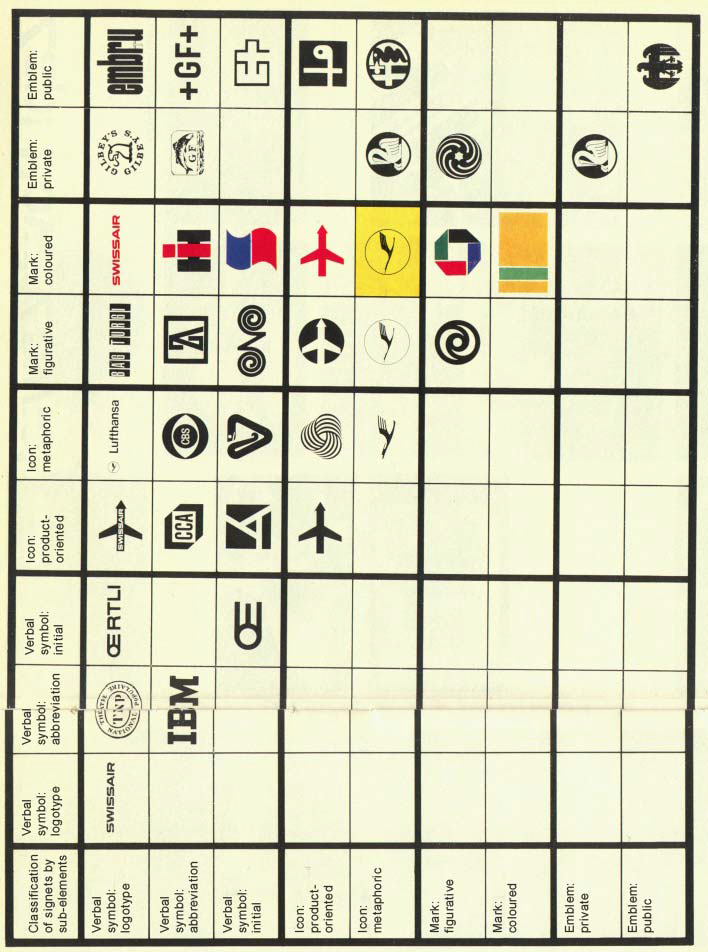
\includegraphics[width=.5\linewidth]{images/wekerle}
  \caption{Классификация Ганса Векерле: симметричная матрица 9 x 9}
  \label{fig:wekerle}
\end{figure}

В комментариях, редактор журнала Design Magazine писал: <<С середины 50-х годов начинается постепенный, хотя часто и совершенно произвольный переход к использованию абстрактных символов для идентификации компании. Они почти полностью вытеснили образные иллюстрации, которые, не смотря на малую информационную ценность, все-таки отличались гуманитарным реалистическим содержанием. Многие из новых символов уже утратили подлинный символический статус и лишены конкретного смысла.  Классификация Г. Векерле детализирует широкий спектр структурных элементов таких символов. Предельно точное описание природы индивидуальных знаков  позволяет создать более функциональный подход, как к  разработке, так и к практическому использованию символики компании, для разных типов предприятий и разных целевых установок.  На сегодняшний день – это первая точная классификация в данной области>>.

Как видим, авторы компилятивных сборников руководствуются главным образом интуицией и желанием найти
оптимальный функциональный принцип сведения всего многообразия логотипов к нескольким простым
доминантам, чтобы затем удобно расположить знаковые кластеры по правилу концентричности. Такие
классификации носят откровенно прикладной характер и ориентированы на то, чтобы быстро информировать
дизайнера, как любителя, так и профессионала, о положение дел в практике лого дизайна на данный
момент.

Более строгий, аналитический подход к классификации логотипов пока встречается крайне редко. По этой
причине любая попытка выйти за пределы наличной эмпирической данности и отрефлексировать накопленный
опыт всегда привлекает к себе особое внимание. Такой пионерской работой можно считать обстоятельное
исследование по истории торговых марок и графических символов П. Моллерапа, в которой он предлагает
семиотический взгляд на родовую классификацию знаков. Обобщив опыт предшественников и современников,
Моллерап подразделяет логотипы (торговые знаки), по признаку функциональности и суггестивной
действенности дизайна, определяя их материальные (то, что торговые знаки изображают) и референтные
(то, что торговые знаки означают) качества. Поговорим об этом чуть подробнее.

Любая классификация, согласно Моллерапу\autocite[][98]{mollerup1999marks}, чтобы соответствовать
своему целевому назначению, должна отвечать следующим критериям:
\begin{enumerate}
\item Идеальная классификация состоит из отдельных групп, между которыми есть чёткая
  граница. Классификация любого объекта должна быть понятна.
\item Критерии, согласно которым строится классификация, должны применяться одновременно. Каждый
  определяющий шаг классификации должен разделять объекты по какому-то одному единому принципу.
\item Выделенные группы одного уровня не должны пересекаться, то есть ни один объект не должен
  принадлежать более чем одной группе.
\item Все группы одного уровня должны охватывать всю совокупность объектов. Любой объект должен
  принадлежать какой-то группе.
\item Формирование групп должно быть обосновано с точки зрения цели построения классификации.
\end{enumerate}

Несмотря не очевидные достоинства такого продуманного подхода, на практике, таксономия, построенная
по этим критериям, как выясняется, объективно не может им следовать до конца. Трудности при
проведении процедур отбора и упорядочения возникают сразу по целому ряду направлений. Первое. Не
всегда возможно провести разделение между группами, т.е. первое и третье правила классификации
вынужденно нарушаются, чтобы выполнялось пятое. Второе. Невозможно установить однозначные границы
между всеми группами одного уровня. Соответственно, заявленные свойства логотипов далеко не всегда
ясны и эксплицитно выражены, а периодически, просто количественны. Третье. Буквы логотипа могут быть
настолько особенными по своей форме, что почти никто не узнаёт в них сами буквы. Объяснение, которое
придаёт смысл логотипу, может быть почти забыто, и для большинства пользователей логотип будет
неявным и даже нереалистичным. Однако свойство используются согласованно, и на каждом шаге
происходит деление только по одному признаку. Четвертое. Группы одного уровня могут
пересекаться. Логотип может содержать одну или несколько букв и картинку, поэтому может и
принадлежать сразу двум группам одного уровня одновременно. Наконец, возможны и другие комбинации
групп. Название может содержать и имя собственное, и обычное безличное имя существительное. Иными
словами, по каждому отдельно взятому свойству таксономия действительно позволяет чётко провести
разделение и упорядочение групп. В то время как на практике свойства, оправдывающие формирование
конкретной группы, зачастую не только не взаимоисключают друг друга, но и проявляются
одновременно. Один логотип может обладать свойствами, присущими двум или более группам.

Тем не менее, в совокупности группы одного уровня действительно покрывают все возможные логотипы
данной категории. Например, если логотип не является графическим, то он и не графический, и т
д. Другим достоинством классификации Моллерапа является тот факт, что она строится на логотипе как
таковом. На его материальных свойствах, на его связи с предметом обозначения, на его референтных
признаках, стилистической пластичности и способности превращения в аллюзию. На самом деле:
материальные свойства логотипа, скорее всего, примерно одинаково воспринимаются большинством
потребителей. При этом культура и культурный контекст, в котором потребитель встречает логотип,
могут значительно варьироваться, что влечет за собой вариативность интерпретаций и, тем самым,
вариативность приписываемых ему референтных качеств.

Из сказанного следует, что один и тот же логотип может быть классифицирован по-разному, и,
следовательно, все классификации логотипа в этой таксономии -- это лишь <<возможные>>
классификации. Номинально исходная классификация Моллерапа представлена двумя семиотическими
категориями (свойства), восемью критериями разделения, семью промежуточными и тридцатью конечными
группами таксономии. Образно она показана в виде дерева (см. Приложение~\ref{app:mollerup}). Корни: \emph{summum genus} -- группа, из которой вырастают надземная
часть дерева. Тринадцать ветвей вправо -- \emph{infima species} -- итоговые группы. В промежутке
находятся \emph{subaltern genera} -- промежуточные группы. Далее, акронимы, сокращения по начальным
и не начальным буквам могут быть дальше разделены как названия, на собственные имена, описательные
имена, метафоры, неочевидные имена и искусственные имена, но это, видимо, слишком. Большая часть
сокращений -- это нарицательные имена. (Подробнее см \autocite[][98-123]{mollerup1999marks}.)
Остановимся здесь.

Итак:
\begin{enumerate}
\item Мы сделали краткий вводный обзор подходов к классификации логотипов по трем направлениям:
  официально-юридическому, неформально-эмпирическому и популярно-семиотическому.
\item Мы постарались показать сходство между этими подходами и проиллюстрировать различия.
\item Основная задача нашего изложения в этой части сводилась к тому, чтобы показать масштабность
  проблемы создания классификации логотипов вообще и создания единой объективной классификации в
  частности.
\item Важное здесь -- неизбежно эвристический характер создаваемых классификаций, их <<возможный>>
  статус. С одной стороны, это объясняется социокультурной обусловленностью чтения логотипов в
  практике жизни. С другой, спецификой деятельности лого дизайнеров, суть которой -- постоянный поиск
  новых идей.
\end{enumerate}

Одним источником вдохновения для лого дизайнеров являются сборники-классификации логотипов,
составленных самими дизайнерами. К разбору одного такого сборника мы и переходим.

\subsubsection{Авторские сборники-классификации}
\label{2.2}

%% TODO: и ещё одна путаница с веками.
На сегодняшний день одним из самых авторитетных сборников\hyp{}классификаций логотипов в профессиональной
среде принято считать два тома визуальной хроники немецкой торговой марки <<A Treasury of German
Trademarks>> (1982, 1985), собранных американским шрифтологом и лого дизайнером Лесли
Кабаргой. Книги представляют собой себя собрание визуальных символов, логотипов, импринтов, обширную
картотеку торговых знаков, созданных в Германии во второй половине XIX в. -- первой половине XX
в. Первый сборник охватывает период с 1850-1925 гг., второй -- 1900-1950 гг.\autocite{cabarga1982treasury}

Думается, выбор Германии в качестве объекта исследования в данном случае вполне закономерен,
учитывая то влияние, которое он оказал на мировую практику лого дизайна в ХХ веке. В совокупности в
сборниках представлены 600 знаков, созданных в Германии в указанный период. Многие логотипы показаны
в двух цветах, как они и были первоначально созданы. Ценность такой подборки, помимо сугубо
исторического значения, состоит и в том, что немецкие логотипы того времени по-прежнему продолжают
жить в современном лого дизайне в виде многочисленных заимствований, цитат, аллюзий, подражаний и
просто как пример красивых безупречно выполненных форм.

В содержательном плане классификация Кабарга включает в себя главным образом личные
идентификационные знаки известных дизайнеров или богатых влиятельных фирм, ценивших стильный дизайн
и имеющих достаточно средств на оплату услуг таких признанных немецких мастеров в этой области как: Карл Шульпиг, Джозеф Биндер, Конрад Йоахим, Ф.Х. Эмке, Людвиг Хольвайн, Люциан Бернхард, Вильгельм Деффке и Карл Эрнст Хинкефус, Рудольф Кох, Вальтер Керстнг, О.Г.В. Хаданк, Филипп Зайц и др. Изобретательность, находчивость и остроумие именно этих дизайнеров Л. Кабарга кладет в
основу своей классификации. С другой стороны, именно эти качества побуждают современных лого
дизайнеров в обязательном порядке приобретать личную копию двухтомника, чтобы иметь ее всегда под
рукой.

Структурно материал сборника организован не по абстрактным категориям, как это обычно принято делать
в классификациях, а по персоналиям и тенденциям. Мы также последуем этому принципу ниже. Но для
начала выборочно представим наиболее ярких представителей немецкой школы лого дизайна.

\begin{enumerate}
\item \textbf{Фриц Хельмут Эмке} (1878--1965 гг.). Кроме создания логотипов, он, как и многие
  немецкие дизайнеры в те времена, занимался архитектурой, дизайном интерьера, плакатов, иллюстрации
  и разработкой шрифтов. Эмке даже придумал своё собственное слово для своих логотипов --
  <<kennbilder>>, которое приблизительно можно перевести, как мгновенно узнаваемая картинка; простой
  дизайн. Тот, который может рассказать историю при одном взгляде на него и при этом находить
  эмоциональный отклик у зрителя. Собственные дизайнерские находки Эмке, в свою очередь, были ни чем
  иным как откликом на орнаменталистику ар-нуво (рисунок~\ref{fig:trademarks:german:emke}).
\item \textbf{Вильгельм Деффке} (1887--1950 гг.), \textbf{Карл Эрнст Хинкефус} (1881--1970 гг.). Оба
  дизайнера входили в ударную группу известной в Германии студии дизайна <<Вильгельмверк>> (1916--1920
  гг.), в начале столетия позиционировавших себя как наследников традиций старых немецких
  мастеров. Фирменный «черный» стиль немецкого лого дизайна сегодня -- наследие творческого успеха
  <<Вильгельмверк>> тех времен (см. рисунок~\ref{fig:trademarks:german:dh}. В то же время, по
  исторической иронии, дизайнерская деятельность этой же студии косвенно ответственна за перерождение
  древнего символа жизненной энергии в нацистскую эмблему немецкого Рейха.
\item \textbf{Карл Шульпиг} (1884--1948 гг.) Один из наиболее часто копируемых немецких
  дизайнеров. Характерная черта его стиля -- органичное сочетание метафорического изображения товара
  с монограммной графикой в вербальной части знака. Возникающий эффект может носить легкий
  иронический характер, равно как и содержать ненавязчивый медитативный подтекст. Тем не менее,
  понять суть его подхода к дизайну непросто. Внешне неброский, стиль Шульпига требует даже от
  имитатора вдумчивого, вникающего отношения (рисунок~\ref{fig:trademarks:german:shulpig}).
\end{enumerate}

%% TODO: и опять век!
Как мы уже отмечали, немецкие логотипы оказали большое влияние на визуальный язык XX века в целом. Германия начала XX века была экспериментальной площадкой для поиска новых нестандартных форм визуальной экспрессии,
принципов композиции и технологии производства. В этом смысле, можно было бы сказать, что самые
талантливые немецкие лого дизайнеры стали частью той широкой и неоднородной традиции, которая
позднее получила название модернизма, провозгласившего разрыв с предшествующим историческим опытом
художественного творчества. Стандартизация технологии производства, базовые принципы, такие как
<<принцип асимметрии, свободы от орнамента, ясности, соответствия духу времени, типографической
самодостаточности (``типографика – не живопись!'') остаются и сегодня в силе>>\autocite[][8]{chihold2011}.

Эстетический протест немецких графиков модернистов был направлен в первую очередь против засилья
тяжеловесных и вычурных форм уходящей эпохи, форм, трудных для быстрого прочтения и не
соответствовавших стремительному духу нового времени. Прежние приемы типографики ориентировались на
медленное, осмысленное прочтение сообщения. Соответственно, вопросы формы и эстетики при разработке
дизайна (выбор шрифта, орнаментов, сочетания шрифтов) имели приоритет перед утилитарной
функциональностью. Так, например, немецкие логотипы XIV-ХVII вв. типично включали в себя элементы
античной мифологии или геральдики -- королевские животные, щиты, мечи и различные комбинации простых
геометрических форм. Подразумевалось, что символическое наполнение логотипа по аналогии
воспроизводит символическое содержание ритуализованных знаков статуса и престижа. Как правило, они
были иллюстративны, сюжетны и описывали некое действо. Для примера: в ХVII в. Германии большой
популярностью пользовались массивные наружные вывески, содержащие реалистичное изображение. Так,
вывеска с именем купца -- Churchill дополнялась изображением церкви и поля, формируя расширенный
ассоциативный ряд для создания символического контекста восприятия знака. В тоже время, в городской
среде широкое распространение получили знаки-вывески прикладного, профессионально-ремесленного
назначения, представлявшие собой простые, стилизованные изображения какого-то ремесла или рода
занятий: очки -- врач-окулист, наковальня -- мастер-кузнец.

Напротив, главной стилеобразующей особенностью немецкого логотипа эпохи модернизма можно считать
выразительную лаконичность его формы и использование древних символов – молнии, креста, стрелы,
животного, птицы. Более того, в начале XX в. немецкая промышленость, ориентированная на массовое
производство товаров, придавала особое значение маркировке своей продукции посредством
логотипа. Часто такой знак был единственным визуальным элементом на упаковке и в рекламном
объявлении. Массовое производство, как отмечалось ранее, порождает массовый спрос, равно как и
создает условия для возникновения массового спроса на услуги лого дизайнера и способствует
формированию массовых профессиональных сообществ дизайнеров, как это и случилось в Германии. Для сравнения, американские логотипы того времени в
основном состояли из названий компаний написанных от руки или же стилизованных изображений
комических персонажей, таких как The Old Dutch Maid, Aunt Jemima, Rastus и
Mr. Peanut \autocite{link:mpr}. Лого дизайн как самостоятельный вид профессиональной деятельности
оформился в США гораздо позже, следуя заразительному примеру инновационного немецкого дизайна и
благодаря регулярным публикациям лучших работ немецких дизайнеров в авторских монографиях и
специализированных журналах, таких как <<Graphis>>, <<Gebrauchsgraphik>>, <<The Studio>>, <<Modern
Publicity>>\autocite{cabarga1982treasury}. Возьмем для примера монографию типографа, дизайнера и педагога Яна Чихольда <<Новая
типографика>>\autocite{chihold2011}, в которой изложены базовые принципы модернистской типографики и
описан функциональный подход к оформлению печатных изданий.

Современный логотип, по Чихольду, должен быть простым и самобытным. Он должен легко запоминаться, то
есть быть узнаваемым и заметным. Как типограф, он убеждён, что хороший логотип совсем не обязательно
рисовать, поскольку эффективный товарный знак можно сделать и типографическим способом. Такой
логотип будет по определению функционален, и <<как и все вещи, выполненные при помощи техники, такой
знак несёт в себе заряд энергии>>\autocite[][118]{chihold2011}. И далее: <<Однако надо серьезно
предостеречь их от того, чтобы называть логотипом простую комбинацию литер из наборной кассы
(монограмму). Логотип -- это нечто совершенно иное, он вмещает в себя гораздо больше смысла, чем
простая монограмма, а плохой логотип гораздо хуже, чем его отсутствие. Сейчас типографы часто
соблазняются возможностью вместо прежних типографских виньеток печатать типомонограммы. Но в рекламе
нужны только логотипы; в наше время монограммы там бессмысленны. Монограмма в качестве фирменного
знака всегда хуже, чем логотип. А плохой логотип может испортить всю рекламную кампанию>>.
\autocite[][119]{chihold2011}

В виде программных требований -- своего рода манифест современного лого дизайна -- эта позиция
оформилась в 1929 году: <<1. Выразительность. Логотип должен выражать качество
продукта. 2. Простота. Логотип должен быть простой, потому что её необходимо будет воспроизводить в
любых размерах и в любой среде. 3. Оригинальность. Логотип не должен быть похожа на другие
трейдмарки. 4. Вневременность. Он не должна возникать из просто модных поветрий. 5. Правильный знак
– основа эффективной рекламы компани>> \autocite{cabarga1982treasury}.

Обращает на себя внимание тот факт, что процитированные слова, сказанные почти столетие тому назад,
по-прежнему звучат свежо и актуально. Представления немецких дизайнеров-модернистов тогда
практически не отличаются от ожиданий и требований к логотипу сегодня. В каком-то смысле, быть
современным всегда -- был, есть и будет главным принципом модернистского мировоззрения. И если
модернизм, в широком смысле, есть <<другое искусство>>, главной целью которого является создание
оригинальных произведений, то лого дизайн в своей модернистской версии -- это <<другой дизайн>>,
базирующийся на внутренней свободе, остраненном видении мира и новых выразительных средствах
изобразительного языка. Само слово \emph{дизайн} означает -- проект, план, замысел. В свою очередь
проект (projectum), следуя логике латинского языка, и вовсе означает -- брошенный вперед\autocite[][323]{serov2005}, что само
по себе роднит немецкий модернистский дизайн с современным ему футуризмом. Футуристы, как известно,
придумывали не только новые слова, профессиональный жаргон, но и язык афиш, и язык плакатов -- язык
рекламы. <<Реклама--– имя вещи\ldots Думайте о рекламе!>>, писал
В.В. Маяковский\autocite{mayakovsky1959}.

Функционализм лого дизайна, т.е. что утилитарно, удобно, то и красиво, естественным образом вытекает
из манифеста художественного объединения Баухаус (1919--1933 гг.), выпущенного в 1919 г. В манифесте, в
частности, провозглашалось равенство между прикладными и изящными искусствами, декларировалось
программное намерение повысить качество выпускаемой продукции в целях удовлетворения массовых
потребностей населения. Для этого промышленные товары нужно сделать красивыми, доступными по цене и
максимально удобными. Иными словами, функциональными.

Другой вопрос, конечно, что функциональная красивость предметов массового потребления, предлагаемых
дизайнерами-модернистами, все-таки не имманентна самому предмету. По сути дела, она свидетельствует
в первую очередь о вкусе и художественном чутье дизайнера.

%% TODO: и опять век!
Таким образом, европейский модернизм в первых двух десятилетиях ХХ века, с его энергичным
стремлением утвердить новые нетрадиционные начала в художественной практике, пропагандой
непрерывного обновления художественных форм и условности (схематизации) стиля, можно назвать первым
значимым источником вдохновения и ориентиром для практики авангардного лого дизайна сегодня. Вторым
важным источником следует назвать <<модерн>> (ар-нуво, югендстиль и т. д.), другое масштабное
направление в европейском искусстве на рубеже ХIХ-XX веков. Модерну свойственно стремление к
сочетанию художественных и утилитарных функций в создаваемых объектах, вовлечение в сферу
прекрасного всех областей деятельности человека, живой интерес к технологиям, отказ от прямых линий
и углов в пользу более естественных, <<природных линий>>. Расцвет прикладных искусств -- еще одна черта
модерна. В том числе и расцвет лого дизайна, как мы отметили ранее, разбирая примеры из сборника
Л. Кабарга.

Таким образом, в самом начале ХХ века логотип оформляется и закрепляется в культуре в виде
концептуального понятия. В современном лого дизайне можно найти достаточно примеров влияний, как
идеологии модернизма, так и философии модерна. В ХХI веке произошли существенные изменения в
техническом решении логотипов. Если раньше логотипы сначала чеканились и рисовались, затем
печаталась, то теперь их дизайн целиком и полностью зависит от того, какое программное обеспечение
для работы с графикой появляется на рынке компьютерных программ. Персональный компьютер как
технология самым решительным образом перестраивают практику графического дизайна и формируют новую
визуальную эстетику. Трудоёмкие зрительные эффекты, оптические иллюзии и сложные градиенты теперь
создаются щелчком мыши, быстро и точно.

Логотипы сегодня изготавливаются серийно и с учетом многочисленных перспективных
носителей. Соответственно повышаются требования к их полифункциональным возможностям. Так, они
должны хорошо читаться в любом диапазоне: в максимально крупных и минимально мелких размерах, любых
форматах и расширениях, включая иконки меню мобильного телефона, URL строки на веб-сайте. Это
касается в равной степени и логотипов в телевизионных программах и широкоформатных кинофильмах, а
также логотипов на любом печатном носителе. В отдельных случаях можно проследить, как
провозглашенная немецкими модернистами лаконичность визуального знака явно вытесняется стремлением к
интенсивной визуальной красивости модерна, наглядно иллюстрируя принцип единства и борьбы
противоположностей. Вместе с тем, как отмечает один из ведущих американских дизайнеров-модернистов
Р. Рэнд: <<You can’t criticize geometry. It’s never wrong.>> Действительно, канонические логотипы NBC,
CBS, PBS, Mobil и др., созданные дизайн студией <<Chermayeff \& Geismar>> еще в середине ХХ века не
подверглись существенным изменениям. Сегодня мы видим их точно такими же, какими они были 50 и более
лет назад.

Подведем черту.
\begin{enumerate}
\item В этом разделе мы вели речь о традиции классификационных сборников логотипов, составляемых
  практиками лого дизайна. Такие сборники, как правило, носят историографический характер и
  выполняют функции профессионального справочника, учебного пособия, документальной хроники
  становления традиции.
\item В качестве примера мы выбрали двухтомное издание американского дизайнера Л. Кабарга, в котором
  задокументирована почти столетняя история немецкой торговой марки (логотипа).
\item Помимо богатого иллюстративного материала, сборники Л. Кабарга содержат ценный
  культурно-исторический комментарий о деятельности немецких лого дизайнеров в контексте своего
  времени -- влияниях, заимствованиях, примерах сотрудничества и кооперации.
\item Мы говорили преимущественно о периоде на рубеже двух предыдущих веков, условно совпадающем с
  функционированием двух несовпадающих художественных направлений в искусстве -- модернизм и модерн.
\item Мы попытались показать, во-первых, как немецкие лого дизайнеры в начале ХХ века активно
  использовали визуальный язык, художественные принципы и приемы работы, характерные для того и
  другого направления. Во-вторых, мы предложили рассматривать современные логотипы, с одной стороны,
  как продолжение сформировавшейся традиции, и как ее преодоление, с другой.
\end{enumerate}

Теперь рассмотрим вопрос о классификации логотипов по темам и мотивам.

\subsubsection{Культурно-историческая классификация}
\label{2.3}

Одним из самых популярных способов классифицирования логотипов следует считать
организацию знаков по принципу ассоциативного ряда. Как правило, структурно
такая классификация представляет собой обширные тематические блоки,
внутри которых кластеры логотипов дифференцируются по тому или иному мотиву --
мифологическому, историческому, культурному, социальному и т.д. За неимением
специального термина мы называет такой подход классификации логотипов
культурно-историческим. Более того, составителями таких компендиумов визуальной
культуры обычно становятся историки и философы, как, например, в случае с
классификацией французских логотипов, разработанной историком Эдит Амиот и
философом Жан-Луи Азизола в 1990 г. и которую мы рассмотрим ниже. Также как
и в случае с авторскими сборниками логотипов, классификация Амиот и Азизола
не претендует на научную объективность. Границы между выделяемыми ими категориями
очень условны, и логотипа одного кластера можно с легкостью помещать в
другую рубрику по другому признаку отбора. Вместе с тем, их подход представляется
чрезвычайно плодотворным, во-первых, в своей познавательной части и, во-вторых,
в части обозначения топографического ареала символических потенций коммерческого
знака-образа. Итак, французский логотип в культурно-исторической перспективе.

С момента зарождения практики регистрации авторского права в 1857 году
Французским Национальным Патентным Бюро, их хранилища сегодня содержат
оригиналы всех зарегистрированных логотипов, счет которым уже давно перевалил
за миллион.

Для своей классификации Амиот и Азизола отобрали 2500
знаков \autocite{edithjeanluois}. Цель отбора --
показать эволюцию экономической деятельности французских корпораций за последние
150 лет в свете изменений социокультурного опыта повседневной жизни в обществе,
в той мере, в какой они отражены в практике графического дизайна в конкретный
исторический период. Материал организован по тематическому принципу. Всего таких
тем -- 27. Внутри каждой темы авторы, помимо представления иллюстративного
материала, предлагают свой комментарий о том, как, по их представлению,
знак-образ суггестивно воздействуют на потребителя. Перечень тем выглядит так:
античность; мифология; аллегории; нечисть; фольклорные персонажи; исторические
личности; Книга Бытия и святые; звезды; растительность; домашние животные;
лесные обитатели; дикие животные; птицы; рыбы; страны; регионы; архитектура;
изображение человека; дети, мужчины, семейные пары; женщины; юмор; предметы и
материалы; антропоморфизмы; труд; транспорт; графичность.

Примечательно, что в классификацию не вошли логотипы-названия фирм, за исключением
тех, которые используют уникальную каллиграфию. Авторы объясняют это тем,
что именно визуальный язык является тем доминирующим фактором, который определяет
качество и надежность <<отпечатка>> в памяти потребителя. В концентрированном виде
логотипы выражают эмоционально окрашенное культурное содержание --
национально-специфичные архетипы коллективной памяти, универсальные символы и
представления о мироздании, понятные всем. По этой причине в лого дизайне
утвердились традиционные темы и мотивы композиции -- сказочные герои, животный
и растительный мир, патриотические сюжеты, призванные помочь установить мгновенную
ассоциативную связь между изображением и припоминаемым (узнаваемым) ассоциативным
комплексом приятных ощущений в лимбической системе головного мозга потребителя.

Связь эта непрямая и в разных случаях призвана решать разные задачи идентификации.
Иногда она может строиться на метафорической связи изображаемого со специфической
деятельностью компании или ее продукцией. Например, логотип компании <<Lacoste>>,
производящей одежду, обувь, парфюмерию и т.д., содержит изображение аллигатора.
Метафора, напомним, это скрытое сравнение, имеющее трехчленную структуру:
\begin{enumerate*}[label=\asbuk*)]
    \item что сравнивается,
    \item с чем сравнивается,
    \item на каком основании сравнивается.
\end{enumerate*}
В нашем случае, предлагается сравнить и обнаружить сходство между водным
позвоночным и деятельностью (продукцией) компании. Основание для сравнения
предлагается сделать самому потребителю. Желаемый ассоциативный ряд, по-видимому,
будет включать абстрактные качества по схеме <<компания такая же\ldots как аллигатор>>.
Например, энергичная, мощная, цепкая, надежная и т.д. Или: наши изделия из
кожи такие же прочные (экзотичные, престижные и т.д.) как кожа аллигатора. Далее,
компания Lacoste не только идентифицирует себя через данную визуальную метафору.
На следующем этапе она предлагает сознанию массового потребителя принять ее
как данность, т.е. перейти от операции сравнения к операции отождествления
желаемого основания для сравнения с именем (имиджем) самой компанией. Метафорические
связи уступают место символическим, метафора трансформируется в символ и миф в
массовом сознании.

Следует заметить, однако, что для знатоков и поклонников тенниса, а именно -- тех,
кто доподлинно знает историю возникновения логотипа Lacoste, знак-образ, с одной
стороны, лишен какой бы то ни было отвлеченной метафоричности. Изображение
аллигатора есть всего-навсего визуальная шутка. Lacoste -- это имя основателя
компании Жана Рене Лакоста, знаменитого французского теннисиста в перво
й половине ХХ века. Во время кубка Дэвиса в 1927~г. капитан французской
сборной по теннису пообещал Рене Лакосту крокодиловый чемодан за победу на турнире.
Турнир он проиграл, но американская пресса мгновенно окрестила Лакоста <<аллигатором>>.
Прозвище закрепилось и даже получило одобрительную символическую интерпретацию,
описывающую его упорное и цепкое поведение на корте. Аллигатор позднее в качестве
личной эмблемы был вышит на блейзере, в котором выступал Лакост. Следовательно,
в сознании потребителя товаров компании Lacoste изображение аллигатора
отождествляется с легендарным теннисистом, становится символом успеха, славы и
престижа. На языке маркетинга -- обещание ценного приобретения, ценности как
таковой, т.е. бренд. Бренд -- это обещание потребного будущего по архаической
суггестивной формуле: <<если\ldots то>>. Если вы будете приобретать наши товары,
то ценные качества, успех и слава героя спорта перейдут к вам.

Соответственно, в классификации Амиот и Азизола обычные знаки-образы прагматичной
самоидентификации объединяются со знаками-образами символического
самоотождествления. К последним следует отнести логотипы, ассоциативно усиливающие
ностальгическое переживание культурно\hyp{}исторического прошлого как более
простого времени, времени более интересного, более нравственного, более
героического и т.д. Ведь логотипу, как и рекламе вообще, совершенно необязательно
показывать сам товар или его производителя. Достаточно создавать настроение,
которое оттеняло бы их привлекательность и вызывало положительные эмоции.
В этом смысле, логотипы создают мемы-ассоциации, формирующие положительное
отношение к деятельности компании и ее продукции. Они продают чувства,
с одной стороны, и обещания привлекательного статуса, с другой. Выборочно
рассмотрим культурную составляющую классификации Амиот и Азиола и снабдим кратким
комментарием. Выделяемые блоки: Античность, Животный и растительный мир, Части света, Изображение человека.

\paragraph{Античность}
Античный стиль очень гармоничный и всегда являлся эталоном для подражания.

Ассоциативная привлекательность образов в их престижности, величественности,
авторитетности, долговечности, историчности и т.д.

\emph{Вавилон}. В 1925 году магазин одежды <<A la ville de Babylone>> выбрал в качестве своего логотипа крылатого быка с человеческой головой, статуи которого когда-то охраняли вход в город в
  Месопотамии (рисунок~\ref{fig:trademarks:french:1.1}).  Знак -- точная копия скульптуры быка, хранящейся в
  Лувре. Аналогично, в 1969 году Дом Ирана в Париже взял в качестве своей эмблемы образ двукрылого
  сфинкса, точную реплику барельефа на покрытом эмалью кирпиче архимедианской эпохи, также хранящемся
  в Париже (рисунок~\ref{fig:trademarks:french:1.2}).

\emph{Греция и Рим}. Культ олимпизма и античных пластических форм как тема лого дизайна вошли в моду
  благодаря Олимпийским играм, проводившихся в Париже в 1924 году. Прославленная красота богинь,
  аскетизм и суровость древних греков и римлян, их несгибаемый дух боевого соперничества породили
  целый вихрь образов, чья красота выражала идею совершенства, мужества, благородства и
  сдержанности. Или более приземленно: Афина Паллада продает пиво (рисунок~\ref{fig:trademarks:french:2.3}),
  Пан, бог пастушества и скотоводства используется в качестве торгового знака для продажи сыра
  (рисунок~\ref{fig:trademarks:french:2.11}), Аполлон убивающий стрелой
  змею на логотипе фармацевтической лаборатории утверждает их намерение покончить со злом в виде
  болезней (рисунок~\ref{fig:trademarks:french:2.10}).

\paragraph{Животный и растительный мир}

В дизайне логотипов зачастую используются изображения растений, животных и птиц,
как цельные формы, так и их метонимические атрибуты. Например, крыло, рога,
силуэты или тени, оттенки шкур. Наиболее распространены символические изображения
животных и птиц, так как у человека в ходе истории сформировались определенные
ассоциации с тем или иным животным, птицей или растением.

\emph{Растения}. Ассоциативная привлекательность образов в их совершенной
  красоте, символическому отождествлению с христианскими добродетелями,
  гармоничностью, выразительностью, стремлением к совершенству, плодородием,
  ростом и т.д.

  Так, в лого дизайне образ трехлистного клевера, символа Троицы, становится
  символом денег, а четырехлистный клевер символом удачи
  (рисунок~\ref{fig:trademarks:french:9.14}). Мотив листа с прожилками часто
  представляет дистрибуционную сеть для сельскохозяйственных продуктов. Цветы
  также способны образовывать прочные связи между товарами, которые они
  представляют, и потребителями. Например, цветочные орнаменты эпохи Арт Деко
  (рисунок~\ref{fig:trademarks:french:9.21}) использовали на мотиве розы.  В
  гирляндах или в качестве бутоньерок розы символизирует природную женскую
  элегантность. Образ дерева, с другой стороны, это прочная опора, в которой
  циркулирует жизненная энергия. Эмблемы, основанные на символе дерева,
  подчеркивают его силу и символическую идею подлинности и уверенности.

\emph{Животные}. Ассоциативная привлекательность образов в безграничных
  возможностях символизации, таких как ощущение тепла и нежности, идеи изобилия и
  плодовитости, качества сообразительности, силы и быстроты, чувства радости,
  веселья, страха и т.д.

  Мотивы животных выделяются едва ли не в каждой книге, посвящённой дизайну
  логотипов. Они легко запоминаются и по этой причине помогают продавать все что
  угодно, как, например, логотип с <<курящим кроликом>>, продающим сигаретную бумагу
  (рисунок~\ref{fig:trademarks:french:10.5}). Известные своей плодовитостью, зайцы и
  кролики обещают изобилие компаниям, выбравшим их для своих логотипов.  Из
  домашней птицы: цыплята символизируют детство, а куры -- материнскую опеку.
  Образ петуха -- самый частотный во французском лого дизайне. Петух также
  является национальной эмблемой Франции, а в функции флюгера на вершине
  церковного шпиля становится величественным выражением патриотического
  единства. Графика изображения французского петуха менялась с течением времени,
  но его можно было всегда опознать по гребню и характерным серповидным перьям в
  хвосте (рисунок~\ref{fig:trademarks:french:10.51}).

  Из других предпочтений: За коровами прочно закрепилась ассоциация с молочными
  продуктами. Исключение составляет успешная марка плавленого сыра <<Vache qui
  rit>> (Смеющаяся корова). (рисунок~\ref{fig:trademarks:french:10.90}). Логотипы с
  изображением овец обычно использовались для продажи текстильных изделий. Собака
  может олицетворять преданность, соперничество и элегантность
  (рисунок~\ref{fig:trademarks:french:10.131},
  рисунок~\ref{fig:trademarks:french:10.138}).  Образ запасливой белки часто
  используется для продажи консервированных продуктов, в то время как еж помогает
  продавать товары для садоводства (рисунок~\ref{fig:trademarks:french:11.6}).

\emph{Птицы}. Ассоциативная привлекательность образов в эстетичности,
  экзотичности, идее полета, свободы, изменения, возрождения и т.д.

  По статистике из всего животного мира именно птиц выбирают чаще всего для
  того, чтобы представить продукт или брэнд. Знакомые виды и экзотические,
  неуловимые и хрупкие, они могут иллюстрировать качества столь противоположные,
  как деликатность и власть. Птичий полет легко представить символом отношений
  между небом и землей. Они олицетворяют собой мечту и освобождение от земных бед
  и неурядиц. У каждого вида свое символическое назначение.  Трясогузка
  (рисунок~\ref{fig:trademarks:french:12.1}) ассоциируется с любовным томлением и
  древнегреческими любовными зельями. Ласточка символизирует изменение,
  возрождение и плодовитость (рисунок~\ref{fig:trademarks:french:12.2}). Морская
  чайка напоминает нам об океане. Плутоватая и болтливая сорока иллюстрирует идею
  баловства (рисунок~\ref{fig:trademarks:french:12.12}) , а голубь символизирует идею
  чистоты души.

\paragraph{Части света}

 Части света -- регионы суши, включающие материки или их
  крупные части вместе с близлежащими островами. Принято выделять шесть частей
  света. Ниже мы говорим только о двух.

\emph{Азия}. Ассоциативная привлекательность образов в экзотичности цветовых
    гамм и восточных мотивов.

    Появление восточных мотивов во французском лого дизайне совпадает с началом
    проведения Всемирных Ярмарок в Париже (1855), на которых экспонировались
    экзотические товары и экспонаты из Азии, достижения колониальной экспансии
    Франции. Только в ХIХ веке в Париже прошло шесть таких ярмарок. Среди логотипов,
    вдохновленных Азией, в основном преобладали японские цветочные мотивы
    (рисунок~\ref{fig:trademarks:french:15.9}), женщины в кимоно, китайцы в
    конусообразных шляпах.  Использовались такие мотивы в рекламе парфюмерных
    товаров, кулинарных специй и пряностей. %(Пример!)

\emph{Африка}. Ассоциативная привлекательность образов в экзотичности далеких
    стран и цивилизаций.

    Если идеализированные образы символизирующие Восток традиционно поэтичны, то
    первые логотипы, изображающие африканцев, носят подчеркнуто расистский
    характер. Широкое распространение получили обезьяноподобные образы чернокожих
    рабов (рисунок~\ref{fig:trademarks:french:15.29}), обряженных в полосатую одежду
    или униформу.  Отношение начинает меняться в 30-е годы ХХ века, в связи с
    нарастающей популярностью американского джаза во Франции. Способствуют этому
    также и научные экспедиции в Африку, открывшие широкой публике глаза на
    самобытность и оригинальность африканского искусства и культуры.  Наконец, успех
    движения за права чернокожих в США (1950-е~--~1960-е) приводит к решительной
    смене настроений в обществе. В лого дизайне на смену образам большегубых
    негритянок приходят атлетически сложенные чернокожие красавицы
    (рисунок~\ref{fig:trademarks:french:15.47}) . Колониальные мотивы в дизайне
    окончательно вытесняются экзотикой другого толка: очарованием далеких незнакомых
    цивилизаций. Зачастую эти мотивы использовалась для продажи ширпотреба: одежды,
    шоколада, мороженого и т.д., постепенно превращаясь в обычные китч-образы,
    свойственные массовой культуре как таковой %(Пример!).

  \paragraph{Изображение человека}

  Изображение человека в логотипе делает его более приветливым, доброжелательным, дружелюбным и таким образом говорит об ориентации в своей работе на человеческий фактор. Такие изображения могут использовать на
    логотипах социальных учреждений, кафе и т.д.

     \emph{Дети}. Ассоциативная привлекательность образов в удовлетворении
      ностальгической потребности взрослых в воспоминаниях детства и потребности детей
      в образцах для подражания.

      Детство -- беспечная пора в жизни человека, ассоциируемая с безусловной
      материнской любовью (рисунок~\ref{fig:trademarks:french:20.22}) и беззаботными
      играми (рисунок~\ref{fig:trademarks:french:20.23}). На детей младшего возраста
      воздействуют образы старших подростков. Они стремятся скорее стать взрослыми,
      добиться признания и уважения у друзей и родителей. Положительную реакцию у
      детей постарше и у подростков вызывают образы кумиров -- известных футболистов,
      музыкантов, или актеров, которым они стремятся подражать.

   \emph{Мужчины}. Ассоциативная привлекательность образов в удовлетворении
      идеальных представлениях о мужественности и семейных отношениях.

      Логотипы с изображениями мужчин в прошлом ориентировались на стереотипные
      представления о мужественности. Мужчины здесь мускулинизированы, полны
      внутренней энергии и решимости. (рисунок~\ref{fig:trademarks:french:20.4})
      Мода ХIХ века диктовала мужчинам необходимость выглядеть солидно и
      импозантно. Напротив, современные логотипы часто ассоциируют мужчин с
      предметами роскоши или исключительными предметами, такими как складной
      цилиндр (рисунок~\ref{fig:trademarks:french:20.7}). Считается, что новый тип
      мужчины полагает, что, потеряв внешний лоск, он компенсирует это ощущением
      истинной силы. Его жена или подруга становятся показателем его достатка и
      вкуса, в той мере, в какой он проявляется в ее красоте и нарядах. По это
      причине современные мужчины на логотипах нередко изображаются в компании
      привлекательных женщин (рисунок~\ref{fig:trademarks:french:20.21}).

  \emph{Женщины}. Ассоциативная привлекательность образов в демонстрации
      идеальных образцов женской красоты и совершенства, грации и пластики,
      элегантности и роскоши, и т.д.

      Образы женщин традиционно представляют бренды, ориентированные
      на предложение товаров для женщин -- гигиенических средств,~косметики, средств
      ухода за волосами, женского белья и проч. В исторической перспективе изменения в
      предложении позволяют проследить этапы развития женской моды, равно как и этапы
      женской эмансипации. Скажем, если женское белье относится к области потребления
      товаров личного или интимного назначения, то такие аксессуары, как макияж и
      духи, участвуют в формировании имиджа женщины на публике. В качестве примера:
      кокетки ХVIII века придумали особый язык мушек, которым активно пользовались как
      орудием флирта. Аналогичную функцию выполняли макияж и духи. В двадцатые годы
      прошлого века женщины начали публично красить губы. Алые губы мгновенно
      появились на логотипах. Самый знаменитый пример -- <<Красный поцелуй>> (риc.~\ref{fig:trademarks:french:21.32}),
      логотип фирмы по производству губной помады. Наконец, образ женщины на отдыхе
      или на работе также повсеместно использовался в лого дизайне. Для продвижения
      бытовых товаров изображались женщины в простых, будничных ситуациях (риc.~\ref{fig:trademarks:french:21.34},
      риc.~\ref{fig:trademarks:french:21.53}). Часто такие логотипы имеют эффект снимка, фотографии. В логотипах одежды
      от кутюр и напитков, наоборот, используются силуэты прекрасных дам. Застывшие
      жесты и торжественные позы символизируют моду и роскошь
      (риc.~\ref{fig:trademarks:french:21.45}, риc.~\ref{fig:trademarks:french:21.52}). Среди
      логотипов этого направления много реалистичных изображений женщин, выполненных в
      стиле эпохи их создания.

Таким образом, мы произвели выборочный разбор классификации логотипов по
культурно-историческому принципу на примере классификации французских
логотипов историком Эдит Амиот и философом Жан-Луи Азизола. Смысл такой
классификации не ограничивается ее культурно-исторической направленностью.
Она также имеет важное практическое значение, поскольку непосредственно
влияет на качество образования и формирования индивидуального графического
стиля современного лого дизайнера. Понятно, что какие-то мотивы, отраженные
в классификации, вышли из употребления вместе с уходом своего времени.
Например, изображение автомобиля вряд ли сегодня может представить в качестве
символа передовой технической мысли. Другие продолжают функционировать,
такие как, например, изображения мифологических существ, животных, растений,
рыб, человека и т.д. Важно то, что логотип здесь представлен полноценным
знаком культуры, документирующим историю не только отдельно взятых компаний,
но и историю определённого исторического периода истории страны. Как и
современный логотип, он отображает ментальность людей, их потребности,
желания и нравы.

Разумеется, в лого дизайне есть примеры и других классификаций,
организующие знаки по их исторической социокультурной наполняемости, как,
например, недавно переизданная коллекция логотипов Эрика Бейкера и Тайлера
Блика <<American Trademarks: From the Roaring '20s to the Swinging '60s>> \autocite{bakerblik2010}.
Это основательная подборка знаков организована тематически по категориям:
дамы и господа, животные, транспорт, круги и формы, ковбои и индейцы,
типографика и, наконец, лица и фигуры. Логотипы учитывают предмет, тему и
форму знака, и предлагают дизайнерам и поклонникам <<американского стиля>>
возможность окунуться в прошлое графического дизайна. Новое издание книги
включает более 1500 известных и менее известных логотипов с 20-х годов
прошлого века и далее, включая современные марки и комментарии известных
дизайнеров. Далее, большой популярностью в профессиональной среде пользуется
двухтомное издание <<Famous Animal Symbols>> (1991) бельгийского дизайнера Пола
Ибоу\autocite{ibou1991}.
Том 1 содержит 266 логотипов животных, получивших мировое признание, и
созданных, по большей мере, профессиональными и хорошо известными художниками,
графическими дизайнерами и рекламными агентствами. Том 2 -- более 250. Тем не
менее, мы остановили свой выбор на историко-культурологической классификации французских логотипов как наиболее полной, детальной и ориентированной на широкий круг
заинтересованных читателей.

Подведем общий итог.
\begin{enumerate}
\item При рассмотрении вопроса о классификации логотипов мы исходили из той
  эмпирической данности, что единой общепринятой классификации коммерческих
  знаков идентификации на данный момент не существует.
\item Трудности создания такой классификации закономерны. Во-первых, сфера
  деятельности лого дизайнера находится в состоянии постоянного обновления и
  изменения. Во-вторых, эклектичный характер технологии создания логотипов
  существенно осложняет процесс отбора общих единых признаков, необходимых для
  формулирования принципов систематизации.
\item Существующие классификации логотипов различаются по функциональному
  назначению, полноте, авторству и принципам систематизации. Большинство
  наличных классификаций созданы для решения практических задач -- закрепление авторского права, обобщение опыта, установление исторической
  преемственности, описание достижений лого дизайна, определение корреляции
  производства логотипов с изменениями в социальной структуре массового
  общества.
\item Разделы \ref{2.2} и \ref{2.3} содержат разборы двух подходов к
  классификации логотипов, обобщающих опыт дизайнерской деятельности в
  Германии и Франции соответственно. В разборе немецкого опыта мы обратили
  внимание на попытку автора поместить деятельность лого дизайнеров начала
  ХХ века в контекст двух широких влияний -- модернизм и модерн. Обе тенденции
  отчетливо прослеживаются в практике лого дизайна сегодня. В разборе
  французского опыта акцент был сделан на культурно-исторический аспект
  изображений на логотипах, популяризирующих те или иные символически насыщенные
  знаки по принципу создания ассоциативных рядов.
\item Мы также предложили различать разные уровни прочтения
  логотипа. К таковым мы отнесли
  \begin{enumerate*}[label=\asbuk*)]
  \item метафорическое прочтение, в основе которого лежит операция
    установления внутреннего сходства по какому-то одному признаку и
  \item символическое прочтение, в основе которого лежит операция
    отождествления знака с тем или иным ассоциативным комплексом.
  \end{enumerate*}
  В первом случае речь идет об игровом отношении к знаку, во втором -- о
  мифотворческом. Обе операции могут находиться в отношениях дополнительности.
\item Наконец, мы уточнили и расширили свое прежнее определение бренда,
  понимаемого как возможное символическое содержание логотипа. Теперь мы
  предлагаем считать бренд суггестивным символом, ориентированным на потребное
  будущее, обещающим значащее повышение качества жизни и самооценки потребителя
  через приобретение рекламируемого товара.
\end{enumerate}

\subsection{Эмблематическая сущность логотипа}

В заключительном параграфе мы обратимся к определению границ семантического поля и социального
статуса логотипа. Номинально логотип, мы говорили ранее, есть общераспространенный знак-переменная
обозначения или маркировки объектов потребления и их производителей. В повседневном общении и в
специальной литературе он может называться товарным знаком, торговой маркой, маркой,
этикеткой-лейблом, символом, брендом и эмблемой.  Отсутствие единого представления о логотипе, с
одной стороны, отражает  субъективное желание пользователей и потребителей наделить знак удобными
или воображаемыми качествами, в целях использования в социально-экономической практике. С другой
стороны, с точки зрения практики лого дизайна, известная произвольность  использования термина
отражает  эклектичность его дизайна и принципов композиции, объективно вытекающих из необходимости
учитывать и удовлетворять желание заказчика. Как показывает опыт, отношение заказчика к выбору
своего логотипа сегодня носит отчетливо выраженный мифотворческий характер. Логотип в данном случае
представляется ему элементом  своего публичного образа или имиджа, тем, что А.Ф. Лосев называет
разрисовкой, картинным излучением личности \autocite[][94]{losev1991}. Для лояльного потребителя
однако логотип, по всей видимости, значим не столько своими мифотворческими потенциями, сколько
тотемической привлекательностью, способностью быть знаком клановой, родовой
принадлежности. Или иначе: знаком принадлежности некоему массовому сообществу. Терминологически
мифотворческие и тотемические возможности логотипа реализуются через его эмблематическую ипостась.
Мы уже рассуждали об исторической связи логотипа с геральдической эмблемой.  Теперь мы рассмотрим
эту аналогию более подробно.

\subsubsection{Границы эмблематического в логотипе}

Эмблематичность представлена в логотипе главным образом тремя свойствами. Во-первых, по внешней
форме исполнения -- сочетание изображения и слова -- логотип может композиционно напоминать
эмблему (рис.~\ref{fig:twins}). Даже в тех случаях, когда мы имеем дело с логотипами, состоящими из
одного вербального элемента или слова (рис.~\ref{fig:maroc}), форма исполнения данного элемента
носит отчетливо выраженный изобразительный характер. Слово-название в логотипе не пишется, а
изображается. Во-вторых, по своей внутренней мотивировке и первоочередному практическому назначению,
логотип, точно также как и эмблема, синхронически может иметь только один фиксированный смысл. В
данном случае: дифференциально обозначать и сигнализировать о присутствии и деятельности
компании-производителя на рынке товаров услуг и предполагаемом высоком качестве ее
продукции. В-третьих, по своему замыслу и основному символическому назначению логотип, подобно
эмблеме, является свернутым мнемоническим блоком, призванный транслировать во времени уникальный
ценностный статус компании-производителя и ее продукции, с одной стороны.  С другой стороны, внушать
целевому массовому потребителю ощущение эмоциональной сопричастности древней традиции, мистически
глубокому, но не до конца понятному смыслу, или, напротив, сопричастность новому технологическому
прорыву, модному тренду, революционному движению в будущее.  Иными словами, однозначность логотипа
во временном континууме предрасположена к энтропии, когда изначально жестко фиксированные внешние и
внутренние связи переформулируются, давая рождение новым смыслам.

\begin{figure}[h!]
  \centering
  
\includegraphics[width=.5\linewidth]{images/twins}
  \caption{Логотип <<Близнецы>>}
  \label{fig:twins}
\end{figure}

\begin{figure}[h!]
  \centering
  
\includegraphics[width=.5\linewidth]{images/maroc}
  \caption{Логотип <<Принц Марок>>}
  \label{fig:maroc}
\end{figure}

Таким образом, логотип и эмблема нетождественны понятийно, и смысловое и формальное сходство между
ними носит лишь временный, этапный характер.  Развернем наши тезисы.

\paragraph{Эмблематическое сочетание}
Современная эмблема – это амальгам формы, образа и имени\hyp{}идентификатора. Она может представлять
собой простое замкнутое построение со стилизованной надписью или изысканно-витиеватым изображением
скрытых смыслов или мотивов. Как таковая эмблема сегодня обычно используются для идентификации
спортивных команд и престижных организаций или корпораций – предположительно, как мы отмечали,  по
аналогии с использованием фамильных гербов средневековой знатью. По своему замыслу современная
эмблема позволяет  массовому потребителю, -- каковым является, в том числе и спортивный болельщик
-- выстроить более тесную коммуникацию с брендом, особенно если она представляют команду или клуб.
С другой стороны, на утилитарном уровне, эмблема выразительно смотрится и на упаковке современных
товаров, как, например, эмблема одного из старейших брендов в Великобритании Lyle’s Golden
Syrup (рис.~\ref{fig:syrop}). С момента своего появления в 1904 году упаковка и логотип компании изменялись
лишь незначительно, придавая имиджу продукции компании значимый и хорошо продающийся ностальгический
статус старинной традиции.

\begin{figure}[h!]
  \centering
  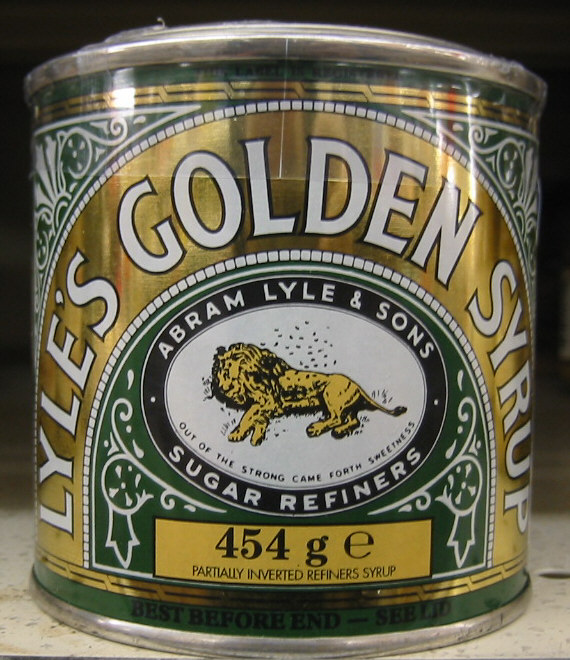
\includegraphics[width=.3\linewidth]{images/goldensyrop}
  \caption{Золотой сироп Лайлс}
  \label{fig:syrop}
\end{figure}

В современной эмблеме соположение вербального элемента и изображения\hyp{}рисунка далеко не всегда
самоочевидно, что само по себе имеет принципиальное значение. Изображение должно сообщать
потребителю нечто иное, не совпадающее и не дублирующее словесное обозначение-подпись. Объяснение
рисунка в эмблеме интерпретатором призвано одновременно как истолковать смысл изображаемого, так и
констатировать семантическую обусловленность изображения и слова. Иначе говоря, оба текста,
изначально представляющие собой разные языки, необходимо приравниваются друг к другу волевым
решением автора, с одной стороны, и интерпретирующим прочтением потребителя, с другой. Эмблема
представляет собой разновидность усиленного фразеологизма,  поскольку за элементами эмблемы
сохраняется право определенной автономии, равно как и возможность образования нового смысла при их
сопоставлении, не равного смыслу каждого из этих элементов в отдельности. Такое сочетание мы
называем эмблематическим. То есть, свободное сочетание некоторого стандартного набора иконических
и вербальных элементов, когда одно и то же изображение может сопровождаться различными подписями, и
одно одна и та же подпись может прилагаться к различным изображениям. Последнее, в частности,
объясняет острую проблему защиты авторского права в лого дизайне, где плагиат и визуальная кража
оригинальных дизайнерских решений носят массовый характер.

Далее, как вербальный, так иконический элементы в эмблеме по объему вмещаемых понятий могут занимать
по отношению друг к другу
\begin{enumerate*}[label=\asbuk*)]
\item обобщающую (свертывающую) позицию и
\item индивидуализирующую (развертывающую) позицию.
\end{enumerate*}
Или проще: по принципу <<свертывание-развертывание>>.  Иконический знак
ориентирован на обозначение единичного, конкретного объекта. Конвенциональный вербальный знак, по
причине своей абстрактности, стремится обозначить любой объект или даже все объекты.

Возникающее внутреннее противоречие оказывается чрезвычайно продуктивным.

Разная природа знаков, составляющих эмблему, позволяет эффективно разрешать его, поскольку в
эмблематическом сочетании значим не сколько логико-семантический объем каждого отдельного
сополагаемого понятия, сколько приведение того и другого к общему знаменателю. Более конкретному,
чем конвенциональный словесный знак, и более абстрактному, чем иконический знак. Если каждая
отдельная составляющая эмблемы может быть многозначной, то их сочетание дает однозначный смысл. По
аналогии с естественным языком, можно было бы сказать, что элементы, образующие эмблему, выполняют
смыслоразличительную функцию, в то время как эмблема в целом -- смыслообразующую. При этом эмблема,
возникающая как результат симметрически замкнутого процесса: от конкретного к абстрактному и снова к
конкретному, может означать только самое себя, т.е. знак с жесткой системой внутренней детерминации
составляющих элементов.

\paragraph{Мнемоническая функция эмблемы}

Из сказанного следует, что эмблема, выполняя свое задание в процессе взаимного указания элементов
друг на друга, оказывается исключительно важным знаком для исполнения ею функции мнемонической
стабилизации смысла. Эмблематический знак, будучи идеальным футляром для памяти, дает возможность
одновременно хранить информацию о некоторых абстрактных свойствах, составляющих ее означаемое, с
одной стороны, и информацию о конкретном объекте предметного мира, потенциально или реально им
соответствующих, с другой. Идея замкнутости, адекватности себе, сопротивляемости переменам, как мы
показали выше, составляет суть эмблемы и позволяет рассматривать ее в качестве механизма хранения
информации. Во всяком случае, еще древние руководства по мнемотехнике советовали запоминать
словесные тексты и абстрактные конструкции, сополагая их с яркими изображениями\autocite[][49]{grigoreva2005}.

Эмблематический по форме прием запоминания использовал, например, И. В. Гете: <<Интересный для него
предмет или местность он набрасывал на бумаге с помощью немногих штрихов, детали же он восполнял
словами, которые вписывал тут же на рисунке. Эти удивительные художественные гибриды позволяли ему в
точности восстанавливать в памяти любую местность (Localitat), которая могла понадобиться ему для
стихотворения или рассказа>>\autocite[][219]{bahtin1979}. Аналогичный
синтетический прием описывает А. Р. Лурия на примере человека, обладающего феноменальной памятью,
для которого наиболее простым способом запоминания словесного текста было последовательное
расположение слов в ряды знакомых с детства образов вдоль какой-нибудь дороги, домов, заборов,
витрин магазинов и т.д. в родном городе \autocite[]{luria1979}.
Примечательно, что механизм памяти срабатывал даже в том случае, когда не
существовало никакой очевидной семантической зависимости между словом и тем объектом, у которого оно
помещалось. Семантическая связь возникает как бы сама собой. Наконец, на основе жизненного опыта,
схожие приемы мнемотехники рекомендует и Д. Карнеги в своих популярных руководствах о том, как
добиться личного успеха в обществе \autocite[][237--420]{karnegi1996}.

Должно быть понятно, что запечатленная в эмблеме информация одновременно является смысловой
единицей. Точнее: единицей одного смысла, при этом непродолжительно действующей единицей.  Символу,
как мы говорили в конце первой главы, свойственно медленное накопление социокультурной памяти.  Его
новый смысл складывается из постепенных незаметных изменений в оттенках значения знака и неизбежно
возникающая при энтропия создает возможность полной трансформации его первоначального
смысла. Напротив, эмблематическое сочетание, по выражению И. Григорьевой, это <<информационный взрыв,
за которым следует полный штиль>> \autocite[][50]{grigoreva2005} В этом ее сильная и слабая стороны. Сильная
состоит в том, что превращает эмблему в готовый блок памяти, который при соответствующих условиях
внедрять в массовое сознание. Такой блок будет убеждать автоматически, практически не оставляя места
для сомнения в правильности предлагаемого высказывания. На этом принципе, как известно, базируется
рекламное сообщение, предполагающее максимально пассивное поглощение готовой информации.  Слабая
сторона выражается в том, что неизбежный распад эмблемы как единицы во времени, при котором
составляющие ее элементы получают возможность независимого функционирования, выводит ее из сферы
строгого эмблематического употребления в сферу стихийного и слабоуправляемого символического
смыслопорождения. Означаемое и означающее здесь зависят в первую очередь от позиции наблюдателя и,
следовательно, носят относительный характер. Логотип, рассматриваемый как часть маркетинговой
стратегии, разумеется, по целевому назначению ничем не отличается от готового мнемонического блока
эмблемы.

\paragraph{Рекламное воздействие коммерческой эмблемы}

Коммерческая эмблема, как и реклама в целом, соблазнительно предлагает массовому
потребителю заместить себя в воображении неким абстрактным, идеальным телом,
получающим наслаждение от вполне конкретных удовольствий. Или же наоборот:
получающим некие абстрактные удовольствия от конкретных товаров потребления.
Эмблемы рекламы по своему психологическому замыслу не должны замечаться сознанием.
Ожидается, что при максимальной пассивности мыслительных процессов в сознании
потребителя, информационный блок незаметно проникает в лимбический центр  мозга
и эффективно формирует перцептивный дубликат-заменитель его реального бытия в
реальном мире. Критичность восприятия блокирует суггестию, как отмечает, например,
М.К.~Рыклин, рассуждая о рекламных изображениях в московском метрополитене:
<<Характерная черта изображений в московском метро -- их незаметность для
протекающей мимо, как бы сквозь них, массы. И это несмотря на их очевидную,
бьющую в глаза фактурность. Превращение этих изображений в объект созерцания --
акт крайне агрессивный, нередко связанный для них с летальным
исходом>>\autocite[][41]{ryklin1992}.
Иначе говоря, рекламную коммерческую эмблему важно не замечать, но необходимо
добиться ее функционирования в качестве привычного естественного фона, как это
видно в следующем примере.

В 2010 году на восемьдесят второй церемонии вручения премии Академии
кинематографических искусств и наук в Лос-Анджелесе в категории <<Лучший
анимационный короткометражный фильм>> премию <<Оскар>> получил французский
мультфильм <<Логорама>> (Logorama). Годом раньше мультфильм получил в 2009 году
премию за <<Лучший короткометражный фильм>> на Стокгольмском кинофестивале и премию
Prix Kodak на кинофестивале в Каннах. Фильм показывает один день из жизни
города-прототипа Лос-Анджелеса, который помимо всего прочего знаменит еще и
тем, что в нем представлено огромное количество рекламы. Действительно, фильм
буквально кишит изображениями логотипов известных компаний, их слоганов и маскотов.
За 16 минут эфирного времени в поле зрения зрителей попадают упоминания примерно
о 2500 компаниях. Здесь практически все является логотипами брендов -- люди,
дома, техника. Имена героев говорят сами за себя: Playboy-кролики,
Linux-пингвины, MGM-львы в зоопарке, Michelin-полицейские выслеживают
преступника по имени Рональд МакДональд, и т.д. В финале мультфильма-боевика
<<Логорама>> клоун-террорист Рональд Макдональд разрушает эмблематичный мир
красивых картинок. Мы видим, что планета, на которой происходят события,
вращается вокруг гигантского логотипа Пепси, а тот в свою очередь висит где-то
на краю логотипа Милки Уэй. Life is better than Milky Way.

В реальной жизни функцию клоуна-террориста, как наглядно продемонстрировали
французские кинематографисты, выполняет критическая рефлексия. Рефлексия убивает
коммерческую эмблему, показывает абсурдность ее претензий, разоблачает
иллюзорность благих намерений и исполнения несбыточных мечтаний. Коммерческая
эмблема, или более узко -- логотип, используемый уже не в качестве знака
маркировки, а в качестве рекламного приема, становится технологией манипуляции
восприятием потребителей, искажения реальности, или попросту --
технологией обмана. Нужно признать, тем не менее, что взятая сама по себе
коммерческая эмблема обманывает ничуть не больше любого другого знака, который
по определению не является тем, на что он указывает.

С другой стороны, как мы неоднократно подчеркивали, свое настоящее значение
знак получает лишь в социальной практике коммуникации, внутри конкретной
сферы его применения. В данном случае такой сферой является реклама. Фабуляция,
гипертрофированное преувеличение и иллюзия имманентны технологии рекламы. Можно
сказать, они являются ее modus vivendi. Современная реклама, превратившись в
повествовательную стратегию, предлагает потребителю уже не столько сам товар,
сколько его идею, имидж, комплекс положительных переживаний (experience),
которые не нуждаются в верификации. Любая произвольно-привлекательная аргументация
может с легкостью рекламировать любой товар. Любой сюжет, миф или ценностная
категория становятся строительным материалом для создания рекламного нарратива
и как таковые отбираются  по принципу эффективного воздействия на целевую
потребительскую массу. Соответственно, рекламный нарратив может быть виртуозным
и изобретательным в использовании приемов ассоциативного творческого
конструирования. В то же время, должно быть понятно, что разнообразие
используемых технических приемов совсем не обязательно предполагает разнообразие
используемых средств и методов. Как раз наоборот: методологически реклама
предсказуема и единообразна, поскольку функционально она соподчинена другой
мощной знаково-символической системе. Эта система называется деньги.

Деньги -- всеобщее меновое средство, безразличное к любым численно не
измеряемым ценностям. Подобно тому, как художник вкладывает все свое мастерство
в написание картины, чтобы превратить ее в деньги, в вещь, ничего общего с
живописью не имеющую, так и копирайтер и лого дизайнер вкладывают свое
мастерство в создание рекламного  нарратива, чтобы превратить его в деньги,
в вещь, ничего общего не имеющую ни с его  содержанием, ни с его художественной
формой. Самый простой вид рекламного продукта и рекламного воздействия
рассчитаны на однократную выгоду, обычно в тех случаях, когда речь идет о
коммерческой рекламе материальных товаров.  Совсем иначе выглядят те
многочисленные случаи, когда рекламные технологии и механизмы переносятся из
сферы сбыта товаров и услуг в социальную жизнь общества с целью формирования
новых потребностей и долгосрочных поведенческих стратегий потребителей.

Речь здесь идет, во-первых, о создании масс лояльных потребителей, объединенных
некоей общей положительной эмоцией, заставляющих их  пользоваться услугами
конкретного продавца, компании производителя или фирмы, независимо от наличия
других, более выгодных предложений. Современного потребителя уже трудно назвать
просто покупателем. Он занимается шоппингом. Между шоппингом и походом в магазин
за покупками есть одно существенное различие. Последнее ориентировано на
приобретение необходимых товаров, удовлетворение материальных потребностей. В
то время как шоппинг – это разновидность социального общения, форма
увлекательного времяпрепровождения вне дома, обычно в торговых центрах, в
компании друзей или членов семьи. Покупка конкретного товара здесь вторична.
Факт покупки не столь значим, как эмоциональный социальный контакт в
сакрализованном пространстве торгового центра, насыщенном образами товаров и
услуг, потребного будущего, равно как и комфортными образцами для
самоидентификации и сравнения. Психологически, иллюзия лучшего будущего,
создаваемая современной рекламной технологией, по-видимому, сходна с иллюзией,
возникающей при прочтении увлекательного романа или просмотра захватывающего
фильма. И в том и в другом случае мы имеем дело с технологией удовольствия и
радости, когерентно произвольной <<пластической силой>>, по определению
А.Н.~Веселовского, способной творить безотносительно к теме, идее или сюжету
предлагаемого нарратива. Логотип как инструмент такой технологии является
эмблематическим фиксатором,  инвариантной точкой, вокруг которой выстраивается
рекламный нарратив. Но, как и любое эмблематическое сочетание, логотип и
реклама утрачивают свою эмблематическую значимость, оказавшись в фокусе
рефлексирующего сознания.

Два уровня рефлексии разрушают эмблематическую конструкцию: что изображается и
как это проверить? Вместе с тем, рефлексирующее сознание по определению не
может быть массовым. Поэтому эмблематические сочетания, к каковым относится
и логотип, успешно выполняют свою мнемоническую функцию анкера в массовом
сознании потребителей, позволяющим эффективно формировать и управлять
потребительскими массами.

Прежде чем перейти к  суггестивным механизмам воздействия, обобщим сказанное.
\begin{enumerate}
\item Логотип подобен эмблематическому сочетанию по структурной сочетаемости
  изобразительных и вербальных элементов, образующих бинарную оппозицию,
  один из членов которой -- образ, изображение -- более предпочтителен, чем второй.
\item В коммуникативном плане, целесообразно различать две ипостаси логотипа:
  \begin{enumerate*}[label=\asbuk*)]
  \item логотип как маркировочный знак идентификации и
  \item логотип как инструмент-технология создания привлекательного имиджа
    производителя, с одной стороны, и имиджа лояльного потребителя, с другой.
  \end{enumerate*}
  Во второй ипостаси логотип становится эмблематическим агентом рекламной
  коммуникации.
\item Подобно эмблеме логотип выполняет мнемоническую функцию в том смысле,
  что представляет собой  готовый блок памяти, внедряемый в массовое сознание
  потребителей. Такой блок становится анкером потребительской активности и
  инструментом формирования массовых сообществ.
 \item Эмблематичность логотипа как коммерческого знака носит временный
  характер, поскольку подвержена энтропии, распаду фиксированного смысла под
  воздействием внешних факторов, таких как, например, склонность массовых
  потребителей к инклюзивному смыслопорождению. Иначе говоря, граница между
  логотипом-эмблемой и логотипом-символом условна и прозрачна.
\end{enumerate}

\subsubsection{Суггестивные механизмы логотипа-эмблемы}

В общем виде мы уже затрагивали вопрос о воздействии (суггестии) в первой главе
в связи с механизмами массообразования. Ниже мы конкретизируем нашу позицию
на материале лого дизайна.

\paragraph{Рекламное воздействие и  проблема внимания}

Воздействие-внушение может быть многоликим и разнообразным. Не будет большим
преувеличением сказать, что в той или иной форме с внушением мы сталкиваемся
повседневно и сами пользуемся им осознанно или неосознанно при выполнении
профессиональных обязанностей, в повседневно общении в семье, на отдыхе, в
кругу друзей и т.д. Наши предпочтения и вкусы зачастую являются результатом
чьих-то влияний, внушений или просто собственного самовнушения. Внушение
заложено в саму природу речевой деятельности и по этой причине распространено
повсеместно и сопровождает нас повсюду. В рекламе воздействие-внушение становится
специально организованным видом односторонней коммуникации, когда восприятие
коммерческой информации не встречает критических барьеров. В то же время,
рекламное внушение -- именно под эти углом зрения мы представляем сейчас
логотип -- принято выделять в особую манипуляторную деятельность, наделяя ее
при этом агрессивными, беспринципными качествами, наносящими непоправимый ущерб
человеческой психике. На самом деле группа рекламозависимых лиц, подверженных
прямому рекламному воздействию, сравнительно немногочисленная. В нее входят
дети, подростки, пожилые люди и больные слабоумием. Взрослый потребитель
воспринимает рекламу критично и осмысленно\autocite{roblesconsumer}.

Идеальная формула рекламного воздействия, сформулированная Дж.В. Лундом в
1947~году -- AIDA (внимание, интерес, желание, действие), показывает
последовательные шаги воздействия на потенциального потребителя. Соответственно
оформляются и задачи такого воздействия: привлечь внимание, вызвать интерес,
способствовать появлению желания приобрести товар, спровоцировать конкретные
действия\autocite{lund1947newspaper}. Реальная жизнь, тем не менее, очень быстро
показала несостоятельность такой схемы. Выяснилось, в частности, что реклама
не только может привлекать внимание потребителей, но также может вызывать и
внутренний протест, равно как и желание приобрести товар совсем не обязательно
приводит к его покупке.

Первая серьезная проблема, с которой сталкивается любой изготовитель рекламы,
это избирательность нашего восприятия. Наш мозг автоматически фильтрует поток
получаемых ощущений, видоизменяя их, отбирая те, которые соотносятся с
предыдущим опытом, с нашими убеждениями, потребностями, желаниями и мнениями.
Мы можем сосредотачивать свое внимание на одних вещах и игнорировать другие.
Скажем, в одном периодическом издании могут быть размещены десятки  рекламных
сообщений, но средний потребитель позднее вспоминает лишь некоторые, в то время
как собственно влияние на него оказывают единицы. Парадокс рекламной
деятельности состоит в том, что рекламодатель, затрачивая миллионные суммы на
свою рекламу в национальных СМИ, на рекламные компании, дизайн упаковки и
оформление товарных витрин, нередко может при последующем опросе оказаться
перед фактом, что мало кто из потребителей помнит что-либо о его товаре и
проведенных рекламных мероприятиях. Более того, некоторые потребители не помнят
ничего. Растущее, как снежный ком, количество моделей и серий товаров и услуг,
казалось бы,  полностью обесценивает усилия копирайтеров и дизайнеров по поиску
уникальных сторон товаров и марок, равно как и  по конструированию незабываемых
ассоциативных комплексов памяти. Во всяком случае, изменение концепции
рекламного образа становится насущной проблемой.

\paragraph{Суггестивные предпосылки рекламного образа}
Традиционное представление о рекламном образе предполагает достоверную
корреляцию между изображением и изображаемым предметом. Но при массовом
производстве похожих товаров становится понятно, что достоверность не может
быть образной, а образность совсем не обязательно должна отражать настоящее
положение дел. В результате, эмблематический по сути рекламный образ отдалился
от рекламируемого предмета, став  одновременно более абстрактным и более
независимым. При этом образность и психологическая дифференциация вышли на
первый план, в то время как качество и убедительность заняли подчинительное
положение. Такое смещение акцентов в рекламной деятельности неожиданно получило
широкий резонанс в гуманитарных науках, в которых -- в крайнем теоретическом
пределе -- современной рекламе приписывается статус идеологической инстанции,
призванной <<оправдывать>> потребление, иррационально воздействовать на умы
граждан и служить апологетом капиталистического общественного устройства.
Согласно этому представлению, в массовом сознании рекламные образы образуют
единое целое и потребляются, ни больше, ни меньше, как фальсифицированная
картина мира, а обладание рекламными вещами создает у массового потребителя
ложное ощущение непосредственной связи с реальностью\autocite[][190-191]{bodriyar1999sistema}.
Несоответствие данного теоретического построения фактам повседневной жизни мы
уже отмечали,  поэтому обратимся непосредственно к техническим механизмам
воздействия в логотипе с точки зрения рекламного сообщения.

\paragraph{Суггестивность эмблематического рекламного сообщения}
Универсальное рекламное сообщение, как мы говорили раньше, носит эмблематический
характер. Если  до этого мы говорили в общем виде о двух составляющих --
изображении и подписи-имени, то теперь введем еще один смыслоразличительный
элемент -- цвет. Все вместе они образуют некую смысловую триаду. Цвет,
по-видимому, является самой простой составляющей. Вполне достаточно знать
закономерности воздействия цвета на психику, чтобы умело им пользоваться.
Можно различать три вида воздействия цвета: физическое, оптическое и
эмоциональное\autocites{tsoygner1971}{serov1997estetika}{kandinsky2001dohovnom}.

\emph{Физическое воздействие}. В данном случае речь идет о воздействии на
  физиологию человека. Сила воздействия зависит от количества цвета,
  его качества, времени воздействия, особенностей нервной системы, пола,
  возраста и прочих факторов. Из обычной палитры известно, например, что
  красный цвет возбуждает нервную систему, вызывает учащение дыхания и
  пульса. Синий цвет, напротив, оказывает тормозящее действие на нервную
  систему. Группа красного, желтого, оранжевого цветов являются цветами
  экстраверсии, т.е. импульса, обращенного наружу. Синий, фиолетовый,
  зеленый, с другой стороны,  интровертивные стимулируют импульсы, обращенные
  внутрь.

  Действие цвета совсем необязательно всегда ассоциативно. Точнее говорить о
  синестезии, т.е. о возбуждение одного органа чувств во время раздражения
  другого. В результате, цвета получают свою особую смысловую интерпретацию.
  Например, желто-коричневый может казаться сухим,  розовый -- слащавым,
  красный -- теплым, оранжевый -- кричащим, фиолетовый -- тяжелым, желтый -- легким.

\emph{Оптическое воздействие}. К этому виду воздействия следует отнести
  оптические явления или иллюзии, вызываемые цветом и изменяющие внешний вид
  предметов. Скажем, светлые цвета, такие как белый или желтый создают эффект
  иррадации. Они как бы распространяются на расположенные рядом с ними более
  темные цвета и уменьшают поверхности, окрашенные в эти цвета. Иррадиация, в частности, играет важную
  роль при конструировании шрифтов. Например, если буквы F и E сохраняют свою полную высоту, то высота
  таких букв как O и G, несколько уменьшаются. В то же время, еще больше уменьшаются буквы A и V из-за
  своих острых окончаний. Эти буквы кажутся ниже общей высоты строки.  Поэтому, чтобы они казались
  одинаковой высоты с остальными буквами строки, их уже при разметке следует вынести несколько вниз
  или вверх за приделы строки.

\begin{figure}[h!]
  \centering
  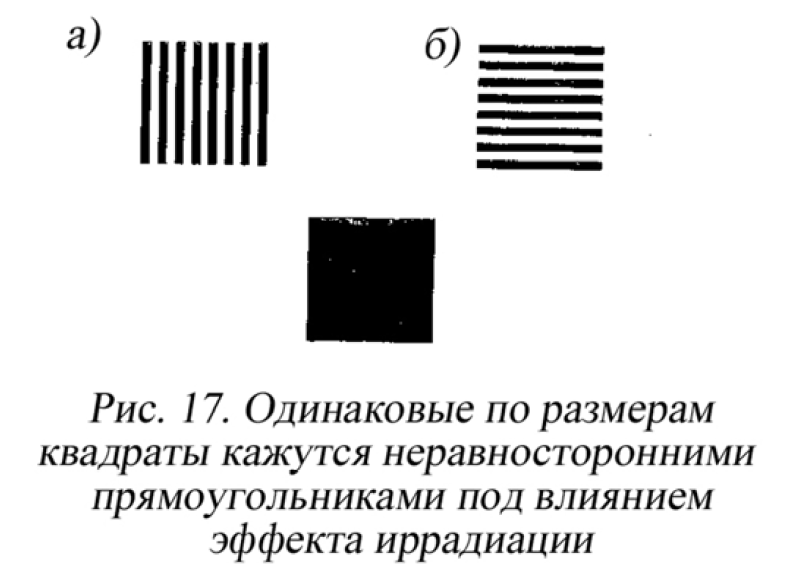
\includegraphics[width=.5\linewidth]{images/irradation}
  \caption{Эффект иррадации}
  \label{fig:irradation}
\end{figure}

  Наконец, эффектом иррадации объясняется и различное впечатление от
  поверхностей, с нанесенными на них продольными или поперечными полосками.
  Поле на рисунке слева (рис.~\ref{fig:irradation}) может казаться более низким, по сравнению с полем на рисунке справа, так как белый
  цвет, окружающий поля проникает между полосками наверху и внизу и визуально уменьшает высоту
  поля. Более обобщенно: желтый цвет зрительно как бы приподнимает
  поверхность, и она может казаться более обширной из-за эффекта иррадации. Если красный цвет
  приближается к нам, то голубой, напротив, удаляется. В то же время как плоскости, окрашенные в
  черный, фиолетовый или темно-синий цвета, зрительно уменьшаются и устремляются к низу.

\emph{Эмоциональное воздействие}. Этот вид воздействия тесно связан с
  оптическими свойствами цвета и говорит о переживаниях и чувствах, которые
  мы можем испытывать под влиянием того или иного цвета. Так, самый спокойный
  цвет -- зеленый. В нем нет движения и никаких признаков ни радости, ни грусти.
  Как таковой он благотворно действует на утомленных людей. Зеленый цвет
  становится более активным и оживленным, если в него ввести желтый. При
  добавлении синего, он, наоборот, делается более серьезным и вдумчивым и т.д.
  Выбор любимого цвета человеком определяется его характером и зависит, помимо
  всего прочего от социальных факторов. Более того характер и выразительность
  цвета может существенно меняться в зависимости от спектра личных ассоциаций.
  Ведь нередко мы пытается объяснить эмоциональное содержание того или иного
  цвета характером предметов, на которых мы обычно воспринимаем этот цвет.
  По этой причине устанавливать здесь какие-либо однозначные правила
  представляется нецелесообразным. Тем не менее, с некоторой вероятностью
  можно предположить, что красный цвет ассоциируется с огнем и страстью,
  желтый -- с солнцем, синий -- с небом или водой, зеленый -- с лесным массивом
  или лугами.

Таким образом, овладев языком цвета, можно выразить и протестный молодежный
максимализм, и подчеркнутый консерватизм, можно сделать образ вульгарным или
нежным, мужественным или женственным и т.д. Изображение и цвет взятые сами по
себе, будучи производными художественного творчества, в рекламном образе
сохраняют известную автономию. Законченный фиксированный смысл по эмблематическому
принципу ему придает подпись-имя или слоган. Внутри эмблематического сочетания
рекламного образа цвет и изображение сужают свой изначальный смысл до намека и
обрамляются вербальным текстом. Важно, что текст не истолковывает точно ни
изобразительные составляющие внутри эмблемы, ни сам рекламируемый предмет.
Вместо этого, триединое сочетание оформляется в виде некой легкой аллюзии, хотя
и по принципу жесткого внутреннего соподчинения, необходимого и достаточного,
как мы говорили, для массового воздействия. Рекламный образ в силу своей
иррациональности и высокой абстрактности означаемого тем не менее эффектно
указывает на некое пусть смутное, но искомое желаемое, с одной стороны, и
создает это желаемое, предлагая в него поверить, с другой.

\paragraph{Суггестивность образа компании в  графической эмблеме}

Образ компании, который несет ее название и графическая эмблема, включает в
себя несколько уровней.

Во-первых, это уровень содержательных ассоциаций. Скажем, название обычно
позволяет строить предположения о профиле компании, даже тогда, когда само
слово-название ничего не значит. Эмблемы, как и названия, могут различаться по
тому, направляют ли они ассоциации в том или ином направлении или вообще не
дают им никакой направленности. Конкретно-изобразительные элементы эмблем,
багет в форме буквы F в логотипе <<French Bakery>> (рис.~\ref{fig:frenchb}) или вешалки в форме куполов
индийского храма в логотипе <<My Indian Closet>>(рис.~\ref{fig:indiancloset}), являются основными носителями
образной информации этого уровня.

\begin{figure}[h!]
  \centering
  \begin{subfigure}{.40\textwidth}
    \centering
    
\includegraphics[width=\linewidth]{images/frenchb}
    \caption{Логотип <<Французская пекарня>>}

    \label{fig:frenchb}
  \end{subfigure}
  \hfill
  \centering
  \begin{subfigure}{.40\textwidth}
    \centering
    
\includegraphics[width=\linewidth]{images/indiancloset}
    \caption{Логотип <<Мой индийский гардероб>>}

    \label{fig:indiancloset}
  \end{subfigure}
   \caption{Ассоциативные эмблемы}
  \end{figure}

Во-вторых, это уровень культурных ассоциаций, по которым можно предполагать
национальную принадлежность и возможно  исторические корни компании. Определенные
ассоциации такого рода могут вызывать не только значащие
названия (<<Чухлома Лес>>, <<Застава>>, <<Пивград>>, <<Серебряная ладья>>), но
и бессмысленные (<<Альфа-Билд>>, <<Modeform>>, <<Воталиф>>, <<Авикос>>).
В эмблеме -- это изобразительные знаки и символы, содержащие в свернутом виде
заряженный эмоциональный опыт и способные непроизвольно воскрешать этот опыт
в подсознании. Это может быть чистая эмоция (Apple), равно как и символ с
общекультурным смыслом (Уроборос). Носителем культурных ассоциаций могут
выступать стилевые элементы или матричные графические фигуры. К последним
относятся, например, круг, крест, свастика, треугольник, закон 10:10,
равно как и базовый <<словарь>>, в который входят тотемные животные, череп,
глаза-окна-зеркала-двери-лестницы-пороги, уши-раковины-трубы-птицы
и~т.д\autocite{link:grigorevalj}.

В-третьих, это эмоциональная окраска звучания названия и изобразительных
элементов эмблемы. При использовании в названии искусственных или иностранных
слов, аббревиатур или акронимов по принципу семантического дифференциала именно
эта сторона выходит вперед. Качества, с которыми звуки подсознательно связываются
в нашем восприятии, могут быть быстрыми и медленными, холодными или горячими,
светлыми и темными, мягкими и жесткими
и~т.д\autocite{juravlev1991zvuk}. В зависимости от преобладания в слове-названии
звуков с той или иной эмоциональной окраской слово в целом тоже приобретает эту
окраску. Графически, точно так же как и звуки, ту или иную эмоциональную
нагрузку несут линии, цвета и другие изобразительные приемы, позволяющие
сделать ощущение знака в восприятии динамичным или устойчивым, легким или
тяжелым, мужественным или женственным и т.д. В то же время, первоначальная цель
графической эмблемы на первом этапе -- не глубокие чувства и переживания, а
фиксация взгляда, ясное и четкое восприятие. По этой причине знак должен быть
одновременно сложным и лаконичным, что достигается обычно через жесткую форму
конструктивного построения, преднамеренную искусственность и четкую геометрию.

Таким образом, в конструировании привлекательного ассоциативного образа компании
широко применяется суггестивная связь используемых выразительных средств с теми
или иными эмоциональными проявлениями. Так, прямые линии  могут выражать одно
состояние, ломаные -- другое, а кривые -- третье. Движение слева направо или
наоборот,  цвета, графические изобразительные формы и звуки речи -- все они
несут в себе те или иные относительно устойчивые эмоциональные значения,
незаметно воздействующие на восприятие массового потребителя, его
эмоционально-чувственную сферу, отвечая его потребностям, желаниям и ожиданиям,
которые по определению являются коллективными. Или иначе: входят в фонд
коллективного бессознательного.

\paragraph{Суггестивнось типического в логотипе}
Концептуально, типическое в логотипе обладает суггестивностью. Суггестивно,
например, повсеместное использование и воспроизведение логотипа на
многочисленных носителях. Подобно тому, как стилистический повтор в риторическом
высказывании рассчитан на оказание воздействия, фиксирует внимание
читателя (слушателя) на той или иной смысловой доминанте, так и логотип,
просто в силу своей повсеместности, своим присутствием непроизвольно
воздействует на потребителя, подчеркивая значимость и значительность
рекламируемого товара и его производителя. Назовем это внешним, эксплицитным
планом суггестии типического. Внутренним, имплицитным планом будет, с одной
стороны, аффектация, т.е. воздействие рекламного образа, вызывающее
кратковременные бурные эмоции. Аффектацию может стимулировать использование
приемов иронии, пародирования, деканонизация общеизвестных эстетических
ценностей. С другой стороны, внутренний план суггестии оформляет  использование
универсальных символов и стоящих за ними природных визуальных паттернов.
Дизайн логотипов в данном случае становится технологией коммуникации через
интуитивное чувство паттерна. Укорененность в природе обеспечивает ему
эстетичность, эффективность и долгосрочность воздействия\autocite[][9]{macnab2008decoding}. Остановимся
на этом подробнее.

К универсальным визуальным паттернам принято относить  круги, свастику, спирали,
разветвления, переплетения и изгибы, треугольники, квадраты и другие многоугольные
фигуры, и числа (1-9). Распознавание паттерна происходит через символ, визуальную
метафору, связанную с природной энергией, которую он выражают. Независимо от
конкретного языка, культуры или исторического периода, такой символ представляет
собой архетип чувства, с которым может идентифицироваться каждый, тем самым
поддерживая связь между глубинным природно-культурным опытом человечества и
современной повседневностью. По этой причине опознавание универсальных символов
и визуальных не вызывает особых трудностей. Проиллюстрируем сказанное на примере
круга, креста, свастики и спирали.

\emph{Круг}. Круги присутствует во многих известных логотипах: NASA, Pepsi,
  AT\&T, Vodafone, Nissan, Volkswagen, BMW и~т.д. В одних случаях окружность
  просто очерчивает контур вокруг слова или графического элемента, работая
  как магический символ, ограждающий от злых сил и хранящий в себе благотворное
  влияние, в других он является формообразующим элементом.

\begin{figure}[h!]
  \centering
  
\includegraphics[width=.4\linewidth]{images/obamademo}
  \caption{Логотип Демократической партии США и логотип Обамы}
  \label{fig:obamademo}
\end{figure}

   Так, например, новый
  логотип американской демократической партии, представленных в рамках нового
  визуального стиля с осени 2010~г. отошёл от традиционного изображения осла,
  раскрашенного в национальные цвета, и стал одной буквой D в круге, а точнее
  в букве O (рис.~\ref{fig:obamademo}). Включенность в круг роднит новый логотип с логотипом
  избирательной компании президента США Б.~Обамы (2008). Логотип Обамы (рис.~\ref{fig:obamademo})
  изображает восходящее над горизонтом солнце нового дня. Образ солнца архетипичен
  и повсеместен в лого дизайне. Такая популярность, вероятно, говорит о том,
  что человечек до сих пор бессознательно сохраняет некоторые следы древнего
  преклонения перед солнцем и реализует эту потребность в современной
  коммерческой символике. Как бы то ни было, логотип-эмблема Обамы и буква О
  положили начало новому тренду в корпоративной айдентике 2011 года.
  Во время новой предвыборной компании на сайте демократов был размещен
  баннер с цифрами 2012, логотипом Обамы в 0 и вопросом <<Are you in?>>,
  что визуально можно перевести <<ты в круге?>> Безусловно, успех логотипа
  Обамы -- это не успех одного только знака. Символом, здесь, скорее,
  является обаятельная, харизматичная личность президента, нежели его
  эмблематический знак. Он -- отражение изменений, произошедших в политическом
  сознании американцев. Значения, которые продуцирует знак, только подкрепляют
  эту идею. В этой связи Обама -- это успешный бренд, который, как и любой
  коммерческий бренд, включает знак, имя бренда, репутацию, атмосферу,
  выстроившуюся вокруг него. Хороший логотип может иметь ценность сам по себе,
  и эта ценность только добавляет к ценности компании, товара или услуги.
  
\begin{figure}[h!]
  \centering
  \begin{subfigure}{.40\textwidth}
    \centering
    
\includegraphics[width=\linewidth]{images/cross1}
    \caption{Религиозный бренд <<Великий Я>>}

    \label{fig:cross1}
  \end{subfigure}
  \hfill
  \centering
  \begin{subfigure}{.40\textwidth}
    \centering
    
\includegraphics[width=\linewidth]{images/cross2}
    \caption{Герб для Надежды Новосадович}

    \label{fig:cross2}
  \end{subfigure}
  \caption{Мотив креста в логотипах}
\end{figure}

\emph{Крест}. Крест -- один из самых успешных универсальных символов, который
  когда-либо существовал. Он мгновенно узнаётся и  имеет большую силу
  воздействия. Первоначально, крест -- символ угнетения и страдания. Крест так
  же являлся атрибутом королевской власти и являлся важной частью
  геральдической символики. А учитывая различные культурные контексты,
  символы Красного Креста, Красного Полумесяца и Красного Кристалла
  используются в различных частях мира, чтобы представлять, что известно в
  Соединенных Штатах как Красный Крест. Использование креста, по своей сути,
  осознается лого дизайнерами, как серьёзный символ и используется
  преимущественно только по прямому назначению, для логотипов религиозного
  характера, или в коммерческой геральдике (рис.~\ref{fig:cross1}, рис.~\ref{fig:cross2}).


\emph{Свастика}. Мы уже упоминали о том, что свастика утратила своё исконное
  значение быть символом жизни, света и благополучия после того, как она была
  тиражирована немецкой дизайн студией <<Вильгельмверк>> и позднее отложилась в
  массовом сознании в качестве эмблемы германского фашизма. До этого свастику
  использовали в качестве символа удачи и счастливой жизни, на предметах быта,
  одежде, гербах и знамёнах, при оформлении храмов и домов, в коммерческих,
  рекламных и пропагандистских целях. Например, в 1925 <<Кока-кола>> выпустила
  <<счастливый брелок>> для карманных часов в форме свастики (рис.~\ref{fig:cocaswastica}).

  \begin{figure}[h!]
  \centering
  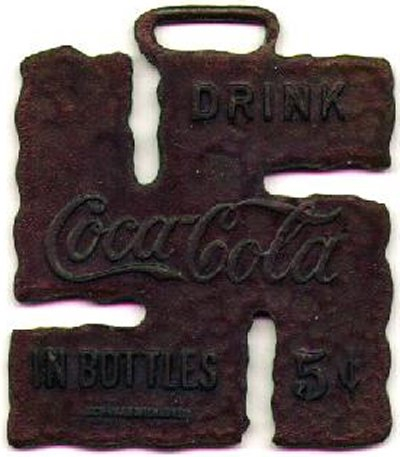
\includegraphics[width=.2\linewidth]{images/cocaswastica}
  \caption{Брелок для карманных часов <<Кока-кола>>, 1925}
  \label{fig:cocaswastica}
\end{figure}

  Сегодня парафразы мотива свастики, помимо эмблем нацистских организаций,
  можно увидеть в логотипах товаров для активного отдыха <<Колумбия>>,
  фоновой фигуре логотипа энергетического гиганта <<Дженерал электрик>>,
  или другого гиганта, компьютерной и программной компании <<Сан Микросистемс>>,
  одного из старейших финансовых конгломератов <<Джей-Пи Морган Чейз>> (рис.~\ref{fig:swastica})
  и т.д. Часто при разработке и утверждении абстрактного графического знака
  схожесть со свастикой может приниматься во внимание.

  \begin{figure}[h!]
  \centering
  
\includegraphics[width=.3\linewidth]{images/swastica}
  \caption{Логотипы <<Колумбия>>, <<Дженерал электрик>>, <<Сан Микросистемс>>, <<Джей-Пи Морган Чейз>>}
  \label{fig:swastica}
\end{figure}

\emph{Спираль}. Спираль является правильным отклонением от круга и воплощает
  в себе идею движения, непрерывного развития и вечного изменения. Спиральные
  формы наблюдаемы в природе в композиции звездной системы, водоворотах и
  смерчах, раковинах моллюсков, папиллярных линиях пальцев и, наконец, в
  двойной спирали ДНК. Спиралевидные змеи изображены на трёх известных
  медицинских эмблемах: посох Асклепия, кадуцей и чаша со змеёй. Так,
  например, жезл Кадуцея символизирует Древо Жизни (связь между небом и землёй),
  двойная спираль из змей -- символ космической энергии, двойственности,
  единства противоположностей, а сами змеи -- плодотворные силы земного и
  потустороннего миров. Золотая спираль в основе золотого сечения -- определяет
  гармоничную пропорцию, лежащую в основе искусства, науки, природы и
  техники. В логотипе <<Белорусского общества биохимии и молекулярной биологии>>,
  например, двойная спираль ДНК представлена в качестве объединяющего мотива
  движения научной мысли и эмблемы жизни на земле (рис.~\ref{fig:biochem}).
  
\begin{figure}[h!]
  \centering
  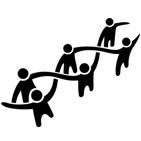
\includegraphics[width=.3\linewidth]{images/biochem}
  \caption{Белорусское общество биохимии и молекулярной биологии. Евгений Рыжанович, Минск}
  \label{fig:biochem}
\end{figure}

Таким образом, мы рассмотрели суггествные механизмы воздействия в логотипе в
той мере, в которой он транслирует рекламный образ компании производителя. По
ходу изложения мы затронули вопросы избирательности внимания, предпосылок рекламного
воздействия, суггестивности эмблематического рекламного сообщения в аспекте
композиции графических образов и ее корреляции с вербальными элементами знака,
в использовании приемов типического в целях усиления воздействия. Главное здесь:
\begin{enumerate}
\item Избирательность внимания существенно усложняет возможность прямого
  рекламного воздействия на сознание потребителя. Более того, современный
  массовой потребитель склонен воспринимать любые рекламные материалы
  критически.
\item Непрямое рекламное воздействие обеспечивается комплексом технических
  приемов, включающих в себя работу с цветовой и звуковой семантикой,
  использование матричных фигур и универсальных символов в композиции
  знака.
\item Внешние формы суггестии становятся возможными благодаря повсеместному
  использованию логотипов-эмблем на различных носителях. Внутренние формы
  суггестии становятся возможными благодаря обращению к приемам аффектации,
  образам и паттернам коллективного бессознательного.
\end{enumerate}

Нам осталось рассмотреть последний и, пожалуй, главный суггестор к которому
апеллирует логотип-эмблема в массовом обществе потребления -- статус.

\subsubsection{Эмблематизация статуса и престижа в логотипе}
Главное требование к логотипу как рекламному знаку -- информативность. Логотип
должен нести информацию о товаре и его производителе. При этом он не нуждается
в рациональном объяснении. Логотипы воспринимаются на бессознательном уровне,
и смыслы их носят коллективный мифологический характер. Рекламный миф,
компонентами которого выступают ценностные предпочтения массового потребителя,
представления о комфорте, благополучии, здоровье, удовольствии, собственности,
власти, славе и т.д., гипотетически потребляется не как искусственно созданный
образ, а как реальность. Восприятие рекламного логотипа подразумевает не только
эмоциональную реакцию потребителей на сам товар как объект эстетического
созерцания, но и их собственные переживания в связи с желанным объектом
потребления, имеющим престижное значение. Иначе говоря, эстетическое
предпочтение потребителей неотделимо от символических значений товаров, обычно
связываемых с их стоимостью или престижностью производителя.

Идентификация и проекция является главными способами воздействия логотипа как
рекламного образа. Идентификация -- это процесс сопоставления себя с другим
человеком, переноса образа другого на себя. Идентификации также свойственны
эмоциональное подражание и способность проекции себя в ситуации и чувства других,
о которых мы говорили раньше. Проекция есть способ, при котором собственные
бессознательные побуждения,  мотивы  и черты, проецируются на других людей
или приписываются им. По этой причине логотип должен быть либо максимально
типичным для целевой аудитории, чтобы запустить процессы идентификации, либо
максимально притягательным, чтобы запустить процессы проекции. Таким образом,
факт приобретения того или иного товара говорит не столько об удовлетворении
потребностей, сколько о желании произвести впечатление на других людей или по
принципу виртуального обладания заполучить некий новый аксессуар, которым обладая
известная личность.

Подражание (имитация) является один из ведущих приемов смыслового наполнения
логотипа как рекламного знака. Подражательный образ отсылает нас к источнику
подражания, тем самым подчеркивая его значимость и ценность. Подражание позволяет
успешно решать рекламные задачи, поскольку <<имитация усваивается легче и
приятнее>>\autocite[][404]{lotman1998iskusstve}. Соответственно, источником
подражания может стать любой признанный образец, который легко воспроизвести,
и в котором запечатлены общечеловеческие ценности. Тем самым имитация позволяет,
во-первых, придать рекламируемым товарам качества и свойства весомых,
художественно значительных, исторически ценных объектов. Во-вторых, блокировать
негативные, нежелательные для потребителя ассоциации.

Рекламные образы логотипов можно группировать по символическому значению
визуального решения
объекта\autocite[][107]{pavlovskaya2003design}. Прием имитации позволят сообщить
товару эмблематичный статус объекта
\begin{enumerate*}[label=\asbuk*)]
\item дорогого и высококачественного;
\item обладающего длительной и славной историей;
\item уникального и рукотворного;
\item признанного и аристократичного;
\item чудесного и мистического.
\end{enumerate*}
Таким образом, престижный статус объекта и проективно -- социальный статус его
обладателя -- образуют единое смысл утверждающее целое, регламентирующее
поведение потребителей на рынке товаров и услуг. Уточним понятие социального
статуса.

Социальный статус -- это положение личности в обществе. Статус может быть
предписанным и не зависеть от усилий личности, и может быть достигаемым, т.е.
может приобретаться вследствие собственных усилий. Он включает в себя оценку
данной личности обществом, так и самооценку самой личности. Если они совпадают,
то это потенциально придает дополнительный импульс личности к развитию, ее
профессиональному и социальному росту, т.е. к повышению своего социального
статуса.

Истрия будущих статусных пертурбаций в социальной структуре общества берет свое
начало в стремительных и радикальных изменениях условий жизни в странах Европы
начиная с конца ХVII века. На тот момент большую часть населения средневековой
и зарождающейся новой Европы составляли крестьяне. У крестьян не было своего
собственного дохода, часто они жили впроголодь, мерзли по причине плохого
отопления,  жили в суеверном страхе и умирали  рано (чаще всего из-за болезней),
не дожив до сорока лет. По окончании жизни, проведенной в нелегком крестьянском
труде, самым ценным нажитым добром в крестьянском хозяйстве оказывались корова,
коза или козел. Но голод всегда был рядом, а болезни -- обычным явлением.
Наиболее распространённые из них: рахиты, язвы, туберкулёз, проказа, абсцессы,
гангрена, опухоли и рак.

Затем, в начале восемнадцатого века, в Британии началось мощное экономическое
преобразование. Благодаря новым сельскохозяйственным технологиям (севооборот,
научный подход к животноводству и консолидация земель) урожай
сельскохозяйственных культур стал резко расти. С 1700 по 1820 годы прибыль
сельского хозяйства в Британии удвоилась, освобождая капитал и рабочую силу,
которые в скором времени переместились в города и включились в развитие торговли
и промышленности. Изобретение парового двигателя и ткацкого станка перевернули
традиционные представления о трудовой деятельности. Города постоянно
разрастались. Если в 1800 году Лондон был единственным городом на Британских
островах с более чем сотней тысяч жителей, то к 1891 году количество таких
городов увеличилось до двадцати трёх. Товары и услуги, которые ранее были
доступны только элите, теперь стали доступными широким массам. Роскошь стала
правилом хорошего тона, а правила хорошего тона -- необходимостью.

Британская потребительская революция набирала темп и расширялась в 19-м веке
по всему западному миру. Гигантские универмаги открывались по всей Европе и
Америке: <<Ле Бон Марше>> и <<Прентам>> в Париже, <<Селфриджес>> и <<Уайтлис>> в
Лондоне, <<Мэйсис>> в Нью-Йорке. Универмаги предлагали обычным людям товары,
которые раньше были доступны только королям. На церемонии открытия нового
двадцатиэтажного универмага в Чикаго в 1902 году, во время разрезания ленточки,
Маршалл Филд, менеджер Гордона Селфриджа, сказал: <<Мы построили это
величественное заведение для обычных людей, чтобы это был их магазин, их дом в
центре города, центр их покупок.>> Он сказал это не для самодовольных
богачей\autocite{debotton}. 

Разнообразие изобретённых технологий не только преобразовало повседневную жизнь,
но и привело к кардинальному изменению картины мира. Прежний циклический взгляд
на мир, когда в следующем году всё должно быть похожим (и таким же неудачным)
на то, что было в предыдущем, сменился уверенностью в том, что жизнь и
человечество в целом теперь может ежегодно совершенствоваться. Таковы предтечи
современных статусных иерархий. Ключевые слова здесь -- смена и изменение.
Вернемся в современность.

Детерминанты статуса, особенно высокого статуса, постоянно меняются вместе с
идеалами общества. По мере того, как различные социальные группы добиваются для
себя большего уважения и признания, они стараются изменить существующую систему,
вступая в противостояние с теми, кому выгоден старый уклад. На сегодняшний день,
в эгалитарном массовом обществе, по аналогии с американским опытом, высоким
статусом  наделяются личности, сумевшие разбогатеть, добиться славы и власти
собственными усилиями. Поскольку современное общество считается в основном
меритократическим, финансовые достижения рассматриваются как заслуженные.

Способность разбогатеть отражает, по меньшей мере, четыре основных достоинства:
способность к творчеству, смелость, практический ум и упорство. Другие
достоинства, как, например, смирение или добродетель, становятся производными.
В отличие от прошлых времен, личные достижения внешне никогда не приписываются
удаче или Божьему промыслу, поскольку сегодняшнему обществу свойственно верить,
что человек способен самостоятельно управлять своей судьбой. В крайнем выражении,
деньги стали мерилом нравственности. Не только наличие денег иррационально
свидетельствует о высоких моральных качествах обладателя, но аналогичную роль
выполняют и разнообразные материальные блага, которые можно приобрести на них.
Если зажиточность говорит о достоинствах человека, то старенький автомобиль и
ветхое жилье заставляют подозревать наличия в нем морального изъяна. Наконец,
деньги обеспечивают доступ не только к высокому статусу, но и к счастью через
приобретение постоянно меняющихся товаров.

На самом деле определяющую функцию денег описал еще Т.~Веблен в <<Теории
праздного класса>> (1899): <<Основа, на которой в конечном счете покоится
хорошая репутация в любом высокоорганизованном обществе, -- денежная сила.
И средствами демонстрации денежной силы, а тем самым и средствами приобретения
или сохранения доброго имени являются праздность и демонстративное материальное
потребление.>>\autocite[][120]{veblen1984teoria}.  Другими словами, в обществе
интенсивного потребления образ порядочного человека несовместим с бедностью.
Соответственно, понятие статусной вещи, дорогого аксессуара, дающего престиж
своему обладателю, базируется на идее, что самое дорогое по карману лишь самым
достойным. По этой причине даже тот, кто лишен материальных устремлений, вынужден
накапливать и показывать свое богатство, чтобы избежать порицания.

Таким образом, обладание большим количеством материальных благ необходимо
современному человеку, не только потому, что они доставляют удовольствие, но что
гораздо важнее -- потому, что они гарантируют уважение окружающих, формируют его
репутацию. Или, выражаясь современным языком, формируют его бренд.

Основная либеральная критика современной идеологии  статуса состоит в том, что
она извращает гуманистические идеалы, отдавая приоритет процессу материального
накопления, который при более сбалансированном подходе должен быть лишь одним
из многочисленных человеческих устремлений. Зрелый подход к проблеме статуса
начинается с понимания того, что статусом человека наделяют социальные группы и
институты: будь то семья, друзья, церковь, артистическая богема, влиятельные
публичные или политические деятели и т.д. В идеале, мы вправе выбрать себе
группу по собственному усмотрению.

Статусный принцип горизонтальной организации социального мобильности в обществе
и сопутствующая ему озабоченность личным статусом, без сомнения, вносит элемент
непредсказуемости и тревожности в жизнь отдельного индивида. С другой стороны,
непросто представить себе благополучную жизнь совсем без него. Страх потерять
лицо или пасть в глазах окружающих, по-видимому, естественно вытекает из здорового
желания успеха, предпочтения одних экзистенциальных обстоятельств другим,
уважительного отношения к Другому.

Социальный статус -- это потребность. Удовлетворение этой потребности в большой
степени есть вопрос индивидуального выбора. Так, ничто не может нам помешать
позаботиться о том, чтобы опасение дискредитировать или скомпрометировать себя в
чьих-либо глазах относилось лишь к кругу тех людей, чью систему ценностей мы
разделяем и чьи критерии оценки мы принимаем. Если статусное неравенство нельзя
отменить, то важно отдавать себе отчет в том, что примыкая к той или иной
инстанции, мы автоматически выбираем одну из возможных иерархических систем
ценностей, по определению противоречащей другим аналогическим системам и
осуждаемой той или иной частью общества. Все это, так или иначе, призвано
напомнить нам: есть разные способы преуспеть в жизни.

Возвращаемся к логотипу. Логотип, будучи рекламным образом, направлен на
удовлетворение потребности в социальном статусе. Он также призван ненавязчиво
напомнить потребителю, что есть разные способы преуспеть в жизни. Воздействие
логотипа сродни воздействию плацебо (от лат. placebo, буквально -- <<понравлюсь>>),
веществу без явных лечебных свойств, лечебный эффект которого до недавнего
времени было принято связывать с верой самого пациента в действенность
препарата.

Последние нейро-исследования, тем не менее, показывают, что плацебо-эффект
основан на бессознательной работе
мозга\autocite{jensen2012nonconscious}.

Мозг принимает решение, как будет воздействовать на нас то или иное лекарство
еще до того, как информация об этом лекарстве будет нами осознана. Рекламные
визуальные образы, соединенные с тем или иным товаром, также работают
терапевтически по принципу плацебо-эффекта, зеркально отражая неосознанные
ожидания потребителя о качестве и статусе коммерческого
предложения\autocite{ariely2009predictably}.

Еще один вклад логотипа в удовлетворение потребности в статусе связан с работой
воображения, исполнением заветного желания, исполнение которого часто сулит
счастье. Логотип романтически обещает исполнение мечты. В идеологическом
дискурсе, в развитие известной американской доктрины, мечта используется для
обозначения идеала жизни <<среднего жителя>>. Автор выражения <<американская
мечта>> историк Дж.Т.~Адамс в <<Эпосе Америки>> (1931) писал об американской
мечте как мечте о земле, где жизнь каждого человека будет лучше, богаче и
содержательнее и где у каждого будет возможность реализовать себя и получить
то, что он
заслуживает\autocite{adams1938epic}. Известно, что Адамс попросил своего
издателя дать книге название <<Американская Мечта>>. Издатель отказался,
аргументировав свой отказ тем, что настоящий американец никогда не потратит \$3.50
на покупку мечты. Адамс попытался возразить, заметив, что настоящий американец
всегда готов отдать за мечту все до последней копейки. Интуитивно Адамс был прав.
Мечта не просто продается, но может продаваться очень дорого. Сегодня это знает любой издатель, копирайтер и лого дизайнер. Индивидуальное и массовое в сознании отдельного человека тесно связаны и взаимно необходимы друг другу. По этой причине мечта о статусе, о счастливом завтрашнем дне, о лучшей жизни всегда будет пользоваться как индивидуальным, так и коллективным (массовым) потребительским спросом.  В культуре потребления этот симбиоз может принимать внешне причудливые формы, соединяющие фундаментальные философские категории бытия и обладания в экстравагантное масскультовое  целое. Так, ежегодный выпуск нового продукта элитной корпорацией  «Apple» традиционно оформляется как масштабное театрализованное уличное действие, привлекающее к участию единовременно  тысячи поклонников и прочих энтузиастов по всему миру. Сюжетную основу  действия образует живая очередь. Очередь перед  входом в фирменный магазин «Apple» начинает формироваться задолго до дня начала продаж, иногда за несколько недель до обозначенного времени. Новый фетишный гаджет -– всего лишь предлог. Шанс развеять хандру и -- пусть на время -- прервать скуку сытой повседневности и одиночества.   Обеспеченные люди разных возрастов приходят группами и в одиночку, чтобы занять место в очереди, чтобы встретить новых интересных друзей, чтобы побыть в массе себе подобных, чтобы совместно переживать бытовые неудобства и лишения бродячего существования, чтобы эмоционально зарядиться позитивной энергией массы, чтобы совместно терпеливо ждать кульминации события живого спектакля.  В другое время, в другом месте и на другом материале С. Беккет обтекаемо назвал такое ожидание <<Waiting for Godot>>.  Словами персонажа знаменитой пьесы: <<Что мы здесь делаем, вот о чем мы должны себя спросить. Нам повезло, что мы знаем. Да, во всем этом ужасном хаосе ясно одно: мы ждем, когда придет Годо. (\ldots) Мы не святые, но у нас назначена встреча. Сколько людей может вам ответить так же?>>.  Ответ напарника: <<Миллиарды.>>\autocite{bekket2009}.

Подведем итог.
\begin{enumerate}
\item В этом параграфе мы попытались представить логотип с точки зрения
  его эмблематической природы. Логотип, мы установили, нецелесообразно
  полностью отождествлять с эмблемой как таковой, поскольку по форме исполнения
  он может принимать самые разные формы.
\item С другой стороны, мы признали, что по признаку сочетаемости
  изобразительных элементов можно вести речь о логотипе как эмблематическом
  сочетании, построенному по принципу бинарной оппозиции.
\item Далее, мы предложили различать две ипостаси логотипа. Если первая
  представляет логотип маркировочным знаком идентификации, то вторая --
  рекламным инструментом-технологией создания привлекательного имиджа
  компании производителя и ее товара.
\item Основной функцией логотипа в рекламной коммуникации является
  мнемоническая. Логотип можно представить в виде готового блока памяти,
  внедряемого в массовое сознание потребителей, где он становится анкером
  потребительской активности.
\item Логотип, понимаемый как эмблематическое сочетание, подвержен энтропии,
  т.е. распаду фиксированного смысла, традиционно присущего эмблеме.
  Разрушение эмблематической структуры в логотипе происходит под влиянием
  внешних факторов.
\item Суггестивные возможности логотипа реализуются как в непосредственной
  практике его применения в рекламной деятельности компании производителя,
  так и в использовании узкоспециальных технических приемов конструирования
  знака. К последним можно отнести, в частности, работу с цветовой и звуковой
  семантикой и т.д.
\item Внутренние формы суггестии -- дополнительный ресурс смыслообразования
  в лого дизайне. К ним относятся, например, использование приемов аффектации,
  образов и паттернов коллективного бессознательного.
\item Психологически, идентификацию и проекцию можно считать главными
  способами воздействия логотипа как рекламного образа. Этим объясняется
  минималистическая эстетика в создании логотипа: максимально типичен или
  максимально притягателен.
\item Имитация является один из ведущих приемов смыслового наполнения
  логотипа как рекламного знака, поскольку имитируемый образ отсылает нас к
  источнику подражания, тем самым подчеркивая его значимость и ценность.
\item Основная смысловая нагрузка, возлагаемая на логотип в общем пакете
  рекламных мероприятий -- придание высокого статуса компании производителю и
  ее продукции, с одной стороны, и потребителю продукции компании, с другой.
\item Мы уделили особое внимание вопросу о социальном статусе как
  направляющей силе социально-экономической жизни современного общества,
  определяющей мотивационно-личностную сферу жизни потребителя сегодня.
\item Исходя из понимания социального статуса как ведущей потребности в
  современном обществе, мы вывели две дополнительные суггестивные функции
  логотипа. Первая функция -- терапевтическая, вторая -- романтическая.
\end{enumerate}

Давление визуальности и визуальной организации опыта в современном обществе, равно как  и сопутствующие им потребительская лихорадка и расширение бессознательного, помещают логотип в разряд эффективных интенсификаторов суггестивности и прочих техник «подсознательного проецирования». Разработка логотипов — это  одна из тех областей графического дизайна, которая может выглядеть простой, но в реальности сопряжена с многочисленными трудностями: как сделать новое, понятное и привлекающее внимание, как соответствовать представлениям анонимного массового потребителя, как захватить его воображение, как обойти разум и/ли скрыть реальную сущность товара. Среди логотипов, вероятно, нет шедевров, поскольку шедевры привлекают лишь немногих, а лого дизайнеру нужно захватить большинство.  В престижном коммерческом знаке массовый потребитель жаждет видеть свой собственный собирательный образ, и логотип предоставляет ему такую возможность.

Повторим основные выводы по главе:
\begin{enumerate}
\item Новое направление в практике лого дизайна – разработка логотипов корпоративной семиотизации объектов  социальной среды в рамках программы глобального брендирования территорий в целях повышения внешней привлекательности конкретного территориального субъекта для индустрии туризма, привлечения инвестиций и модернизации инфраструктуры города или территории.
\item В лого дизайне социокультурного назначения обращают на себя внимание следующие тенденции: а) использование культурно-исторического потенциала места б) его географического потенциала в) создание новых знаков (абстрактных, типографических, монограмм).
\item Существующие классификации логотипов различаются по функциональному назначению, полноте, авторству и принципам систематизации. Большинство наличных классификаций созданы для решения практических задач, таких как закрепление авторского права, обобщение опыта, установление исторической преемственности, описание достижений лого дизайна, определение корреляции производства логотипов с изменениями в социальной структуре массового общества.
\item Следует различать два уровня прочтения логотипа: а.) метафорическое прочтение, в основе которого лежит операция установления внутреннего сходства по какому-то одному признаку  и б.) символическое прочтение, в основе которого лежит операция отождествления знака с тем или иным ассоциативным комплексом. В первом случае речь идет об игровом отношении к знаку, во втором – о мифотворческом. Обе операции могут находиться в отношениях дополнительности.
\item По признаку сочетаемости изобразительных элементов  логотип представляет собой эмблематическое сочетание, построенное по принципу бинарной оппозиции или интерфейса – «границы раздела», обозначающих встречу и преобразование двух структур.
Две ипостаси логотипа: а.) маркировочный знак идентификации, б.) рекламный инструмент-технология создания привлекательного имиджа компании производителя и ее товара. Основной функцией логотипа в рекламной коммуникации является суггестивно-мнемоническая. В виде готового блока памяти он внедряется в массовое сознание потребителей, становясь анкером потребительской активности.
\item Идентификацию и проекцию можно считать главными психологическими способами воздействия логотипа как рекламного образа. Этим объясняется минималистическая эстетика в создании логотипа: максимально типичен и/ли максимально притягателен.
Имитация является один из ведущих приемов смыслового наполнения логотипа как рекламного знака, поскольку имитируемый образ отсылает нас к источнику подражания, тем самым подчеркивая его значимость и ценность.
\item Основная смысловая нагрузка, возлагаемая на логотип в общем пакете рекламных мероприятий – придание высокого статуса компании производителю и ее продукции, с одной стороны, и потребителю продукции компании, с другой. Исходя из понимания социального статуса как ведущей потребности в современном обществе, мы вывели две дополнительные суггестивные функции логотипа. Первая функция – терапевтическая, вторая – романтическая.
\end{enumerate}

\section*{Заключение}

В кинофильме <<Новые времена>> (Modern Times, 1936) асоциальный герой Чарли Чаплина становится
фабричным рабочим Электросталелитейной компании, затягивающим болты на ленте быстродвижущегося
конвейера. Хозяин-капиталист наблюдает за производственным процессом с помощью скрытой камеры и
постоянно требует увеличения скорости линии. Чарли не поспевает за темпом и в нервном истощении
падает на гигантские шестерни. Рабочее название <<Новых времен>> -- <<Массы>> (Masses).  Одна из
основных тем фильма -- конфликт между человеком и массовым обществом индустриального
капитализма. Кроме того, в фильме выразительно представлены и совмещены главные символы
современности -- механизированная фабрика и крупный универмаг, в котором продаются товары массового
производства.

<<Новые времена>> в конце ХIХ и первой половине ХХ века означали склонность к социальной инженерии,
преклонение перед техникой,  ускорение темпов жизни и уменьшение расстояний.  Но прежде всего <<новые
времена>> означали выход <<масс>> на историческую сцену. Массовое производство, массовое общество,
массовая культура выросли из новых технологий, в то время как массовое сознание оформилось благодаря
появлению новых информационных средств. Массовое производство породило массовое потребление, которое
одновременно является и источником, и продуктом массовых форм их удовлетворения.  Но если массовое
производство есть процесс стандартизации предметов производства, запуск на конвейер одинаковых
вещей, то именно массовое потребление распространяет процесс стандартизации не только на
производство, но и на все сферы жизни, подводя под единый стандарт вкусы, привычки, поведение, образ
мысли потребителей, независимо от уровня образования, профессиональной занятости и т.д.

Процессы омассовления можно рассматривать двояко. С одной стороны, они приводят к усреднению,
нивелировке образа жизни всех слоев населения в обществе. С развитием технологий массовой информации
сегодня речь идет уже не просто о массовом читателе, слушателе или зрителе, а об универсальной
публике, повсеместно потребляющей одинаковую информацию, смотрящей одинаковые фильмы, слушающей
одинаковую  музыку и т.д. Традиционные границы в культуре  разрушаются, и сама культура превращается
в товар. Влияние переходит от индивидуальных вкусов к авторитету рынка. Масс-культурная модель
современного общества, по выражению Дж. Сибрука, есть модель <<ноубрау>> (Nobrow), в которой
коммерческая культура супермаркета -- многогранный источник статуса и престижа. В культуре
супермаркета, в отличие от вертикальной иерархической культуры, ценность определяется не столько
качеством, сколько аутентичностью, принадлежностью к доминантной субкультуре или культу \autocite[][74]{sibruk2005}.

Другой взгляд на глобальную массовизацию современной жизни подчеркивает ее демократический
характер. Согласно этой позиции, массовое производство и массовое потребление объективно говорят о
преодолении социального неравенства, об улучшению материального качества жизни членов общества, о
возвращении в аудиальный мир одновременных событий и всеобщего сознания. Энди Уорхол, основатель
поп-арта, суммирует это следующим образом: <<Ты смотришь телевизор и видишь кока-колу, и ты знаешь,
что Президент пьет кока-колу, Лиз Тейлор пьет кока-колу и только подумай -- ты тоже можешь пить кока-колу. Кока-кола есть кока-кола, и ни за какие деньги ты не купишь кока-колы лучше, чем та, что пьет
бродяга на углу. Все кока-колы одинаковы, и все они хороши. Лиз Тейлор иэто знает, Президент это
знает, и ты это знаешь.>>\autocite[][94]{warhol2002}. 

Логотип есть универсальная письменная технология, визуальный код знаковой организации визуальных
элементов в целях выделения товара или услуги среди множества других конкурирующих товаров или услуг
на рынке. В замкнутой системе рекламной коммуникации логотип -- это инструмент стандартизации и
визуальное средство однотипной потребительской информации. Это также оригинальное изображение
наименования фирмы или направления ее деятельности. В функции идентификатора логотип может быть
максимально конкретным и предельно абстрактным по форме исполнения. В рекламной функции визуальной
репрезентации бренда логотип, будучи письменным знаком, абстрактно иллюзорен. Как и любая визуальная
технология он лишен элемента личной обращенности и может быть интерпретирован так или иначе, по
желанию. В то же время наиболее существенной чертами прагматики логотипа являются его
воспроизводимость и повторяемость. Повторяемость ведет к гипнотическому воздействию и
суггестии. В этом смысле логотип способствует не столько продаже товара потребителю, сколько
продаже потребителя товару. Современный товар не становится лучше или проще, но, напротив,
регрессирует и опрощается потребитель, некритично смотрящий на мир как исключительно визуальное
пространство.

Изобретенные в середине XV столетия способы точного воспроизведения изобразительных сообщений с
помощью разборного типографического шрифта стали одним из важнейших орудий современной жизни и
мысли. Современный логотип -- этимологически  понимаемый как <<отпечаток слова>>  или текстовое
клише -- значимое развитие старой техники печатания. Повсеместность и тотальность его использования
в изображениях товарных знаков и статусных эмблемах  делают логотип знаковым социокультурным
явлением в визуально организованной жизни современного общества потребления. Тем самым логотип не
столько отражает или выражает массовое сознание, сколько его формирует.  В этом заключается его
эмблематическая сущность -- быть штамповым следом логоса. В легко узнаваемой однородности,
повторяемости и типичности заключается сила его массового воздействия.

Ч. Чаплин в интервью 1966 года рассуждает: <<Я не боюсь штампов, если они правдивы. Вся жизнь –
штамп. Мы все живем, и умираем, и едим три раза в день,  и влюбляемся, и разочаровываемся. (\ldots)
Люди, как говорится, делали это и раньше. Ну и что же из того? Если избегать штампов, то станешь
скучным.>>\autocite[][138]{chaplin2005}.

В финальной сцене <<Новых времен>> мы видим парочку, бредущую вниз по опустевшей дороге после
очередного увольнения -- но рука об руку. <<Маленький человек>>  Чарли Чаплина снова оказывается в
трудных обстоятельствах, но он ничуть не обескуражен. Даже торжествует.

\end{onehalfspace}

% ------------------------------------------------------------------------------
% Список литературы
 \begingroup
\sloppy
\printbibliography{}
\endgroup

% ------------------------------------------------------------------------------
% Приложения

\begin{appendices}
  %% Согласно ЕСКД, номер рисунка в приложении должен содержать номер приложения.
  \counterwithin{figure}{section}
  \counterwithin{table}{section}
  \renewcommand{\thesection}{\Asbuk{section}}

 \section{Logo Trends}
\label{app:logotrends}

 \appendix
\section{Emblemetrics}
\label{app:emblemetrics}

\begin{figure}[ht]
  \centering
  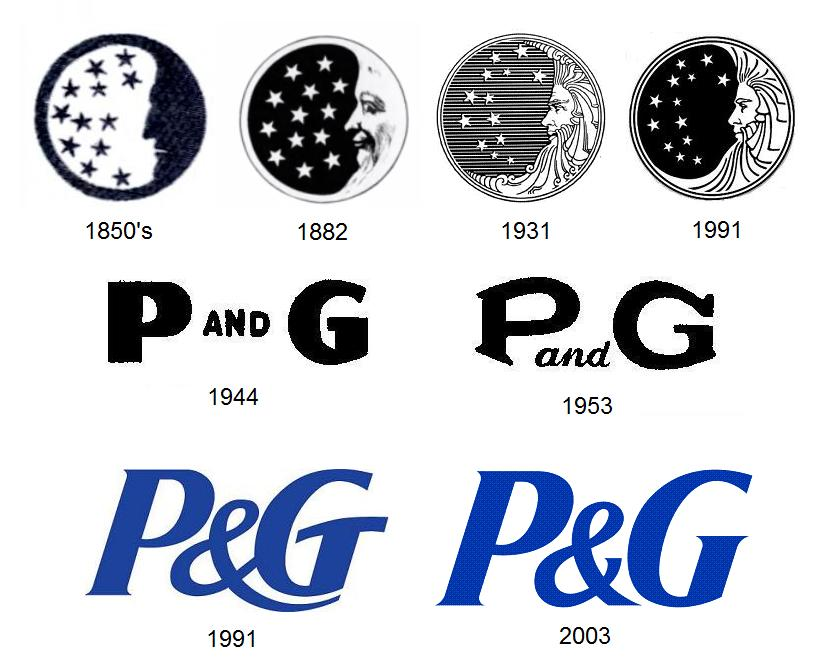
\includegraphics[width=.5\linewidth]{images/supplement/emblemetrics/pg2003}
  \caption{Логотипы P\&G до 2003}
  \label{fig:emblemetrics:pg2003}
\end{figure}

\begin{figure}[ht]
  \centering
  
\includegraphics[width=.5\linewidth]{images/supplement/emblemetrics/pg2013}
  \caption{Обновлённый логотип P\&G 2013}
  \label{fig:emblemetrics:pg2013}
\end{figure}

\begin{figure}[ht]
  \centering
  
\includegraphics[width=.5\linewidth]{images/supplement/emblemetrics/frankenmarks}
  \caption{Frankenmarks}
  \label{fig:emblemetrics:frankenmarks}
\end{figure}

\begin{figure}[ht]
  \centering
  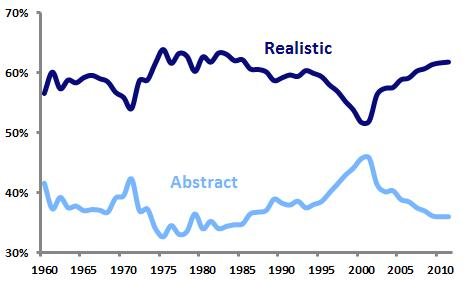
\includegraphics[width=.5\linewidth]{images/supplement/emblemetrics/abstractrealistic}
  \caption{Abstract and realistic logos as a percentage of all new US logos}
  \label{fig:emblemetrics:abstract-realistic}
\end{figure}

\begin{figure}[ht]
  \centering
  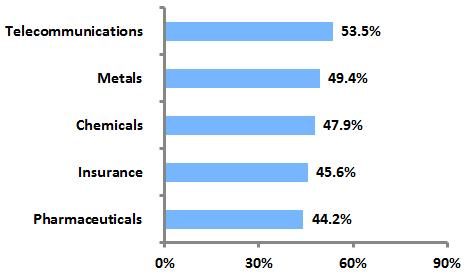
\includegraphics[width=.5\linewidth]{images/supplement/emblemetrics/highabstract}
  \caption{Industries with high rates of abstract logo use}
  \label{fig:emblemetrics:high-abstract}
\end{figure}

\begin{figure}[ht]
  \centering
  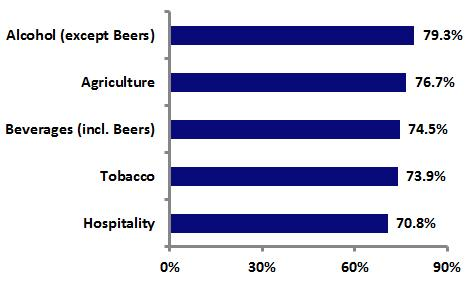
\includegraphics[width=.5\linewidth]{images/supplement/emblemetrics/highrealistic}
  \caption{Industries with high rates of realistic logo use}
  \label{fig:emblemetrics:high-realistic}
\end{figure}

\begin{figure}[ht]
  \centering
  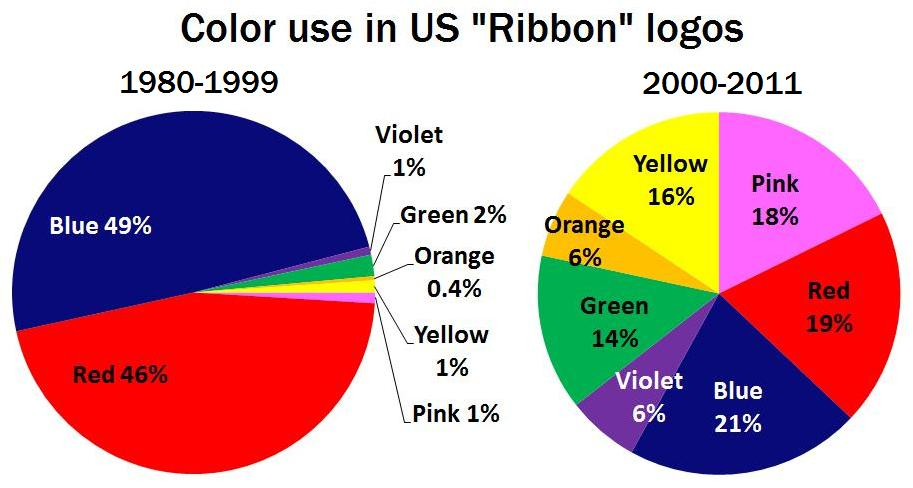
\includegraphics[width=.5\linewidth]{images/supplement/emblemetrics/coloruse}
  \caption{Color use in US Ribbon logos}
  \label{fig:emblemetrics:color-use}
\end{figure}

\begin{figure}[ht]
  \centering
  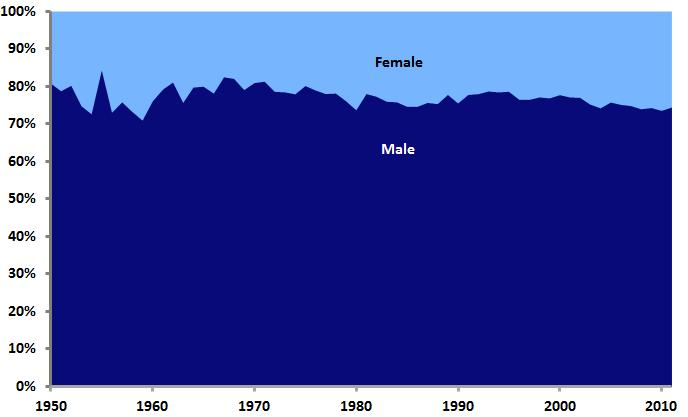
\includegraphics[width=.5\linewidth]{images/supplement/emblemetrics/malefemale}
  \caption{Percentage of new <<gendered>> logos featuring male or female design elements}
  \label{fig:emblemetrics:male-female}
\end{figure}

\begin{figure}[ht]
  \centering
  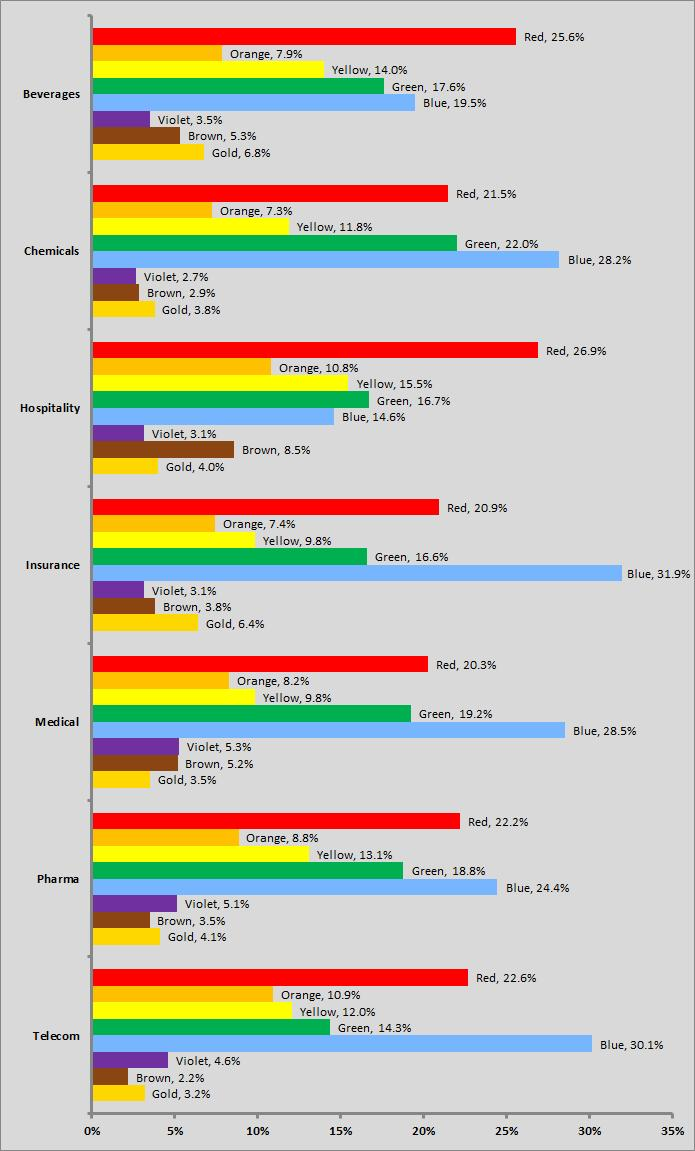
\includegraphics[width=.5\linewidth]{images/supplement/emblemetrics/colorindustry}
  \caption{Use of Color in US Logos by Industry}
  \label{fig:emblemetrics:color-industry}
\end{figure}

\begin{figure}[ht]
  \centering
  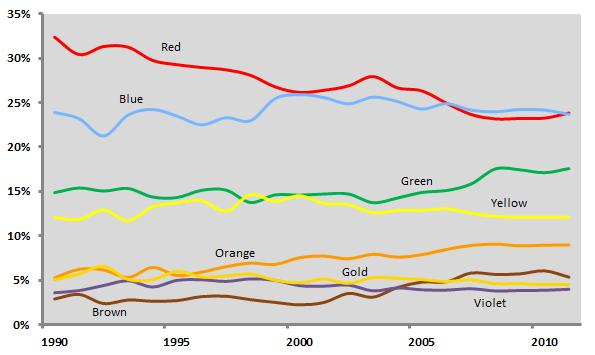
\includegraphics[width=.5\linewidth]{images/supplement/emblemetrics/color}
  \caption{Use of Color in US Logos}
  \label{fig:emblemetrics:color}
\end{figure}

\begin{figure}[ht]
  \centering
  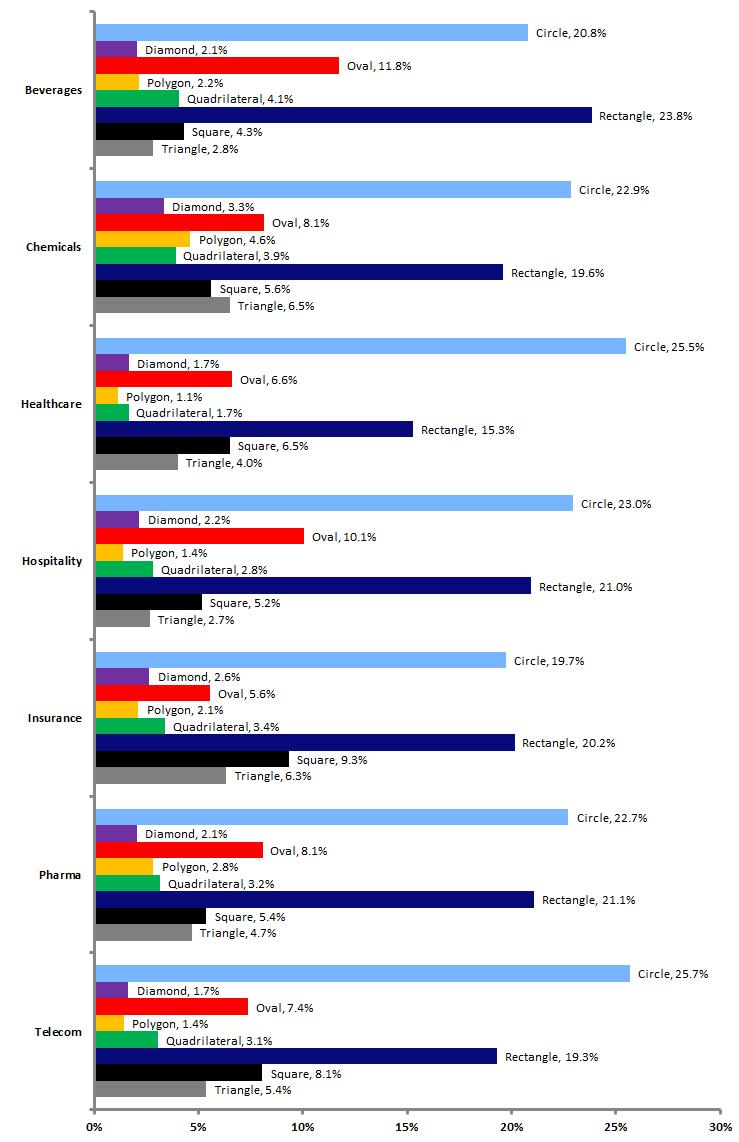
\includegraphics[width=.5\linewidth]{images/supplement/emblemetrics/shapeindustry}
  \caption{Percentage of logos featuring shape elements by industry}
  \label{fig:emblemetrics:shape-industry}
\end{figure}

\begin{figure}[ht]
  \centering
  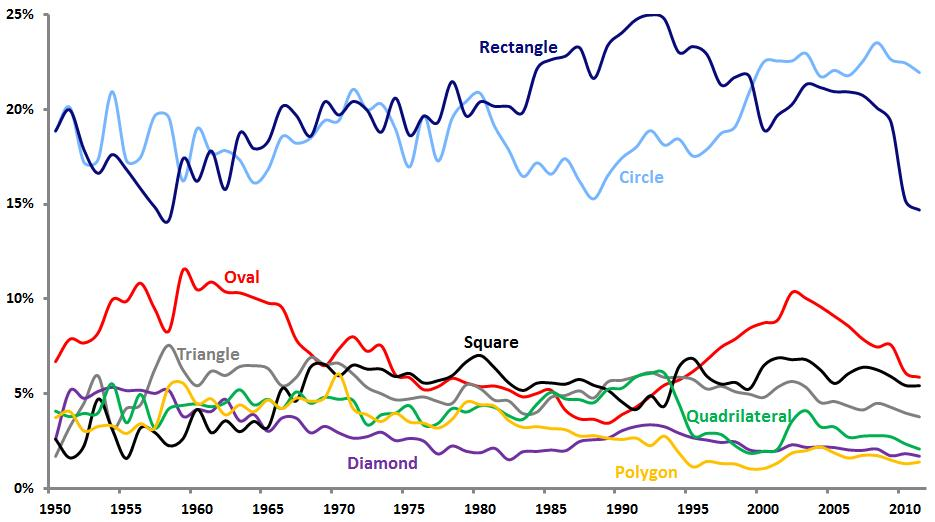
\includegraphics[width=.5\linewidth]{images/supplement/emblemetrics/shape}
  \caption{Percentage of new logos featuring specific shape elements}
  \label{fig:emblemetrics:shape}
\end{figure}

\begin{figure}[ht]
  \centering
  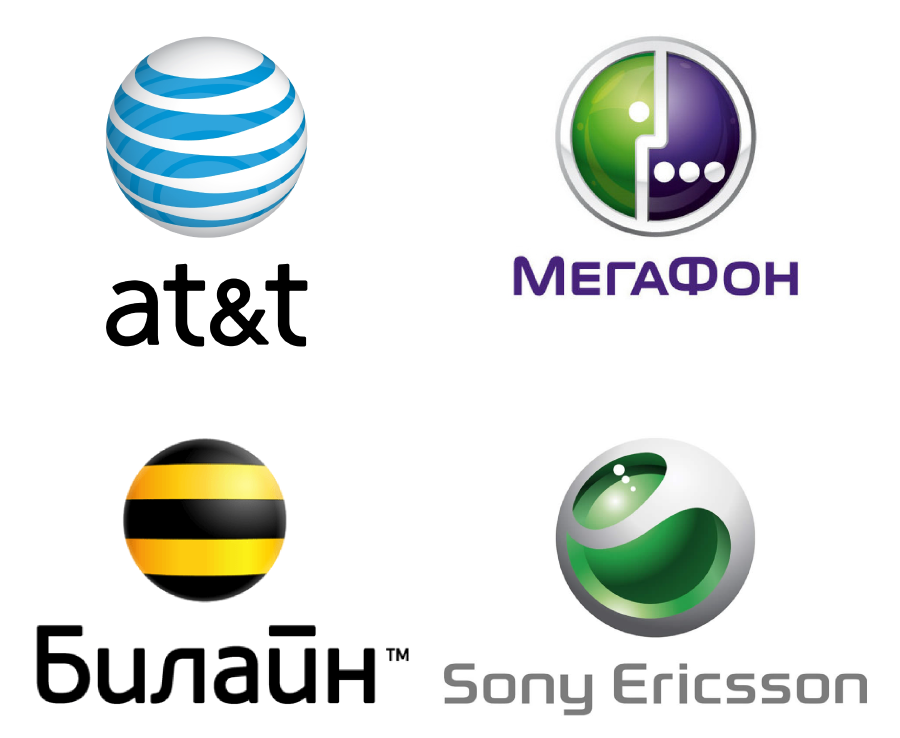
\includegraphics[width=.5\linewidth]{images/supplement/emblemetrics/web20}
  \caption{Логотипы операторов сотовой связи, выполненные в стилистике веб 2.0}
  \label{fig:emblemetrics:web20}
\end{figure}

 \section{Территориальный брендинг}
\label{app:territorial}

\begin{figure}[ht]
  \centering
  
\includegraphics[width=.3\linewidth]{images/supplement/territorial/ny}
  \caption{Логотип-слоган <<I love New York>>, Милтон Глейзер, 1977 г.}
  \label{fig:territorial:ny}
\end{figure}

\begin{figure}[ht]
  \centering
  
\includegraphics[width=.5\linewidth]{images/supplement/territorial/moscow}
  \caption{Логотип сети книжных магазинов <<Москва>>}
  \label{fig:territorial:moscow}
\end{figure}

\begin{figure}[ht]
  \centering
  
\includegraphics[width=.5\linewidth]{images/supplement/territorial/melbourne}
  \caption{Ребрендинг Мельбурна (Австралия), дизайн Джейсон Литтл, Landor Австралия}
  \label{fig:territorial:melbourne}
\end{figure}

\begin{figure}[ht]
  \centering
  
\includegraphics[width=.5\linewidth]{images/supplement/territorial/amsterdam}
  \caption{Амстердам}
  \label{fig:territorial:amsterdam}
\end{figure}

\begin{figure}[ht]
  \centering
  
\includegraphics[width=.5\linewidth]{images/supplement/territorial/copenhagen}
  \caption{Копенгаген}
  \label{fig:territorial:copenhagen}
\end{figure}

\begin{figure}[ht]
  \centering
  
\includegraphics[width=.3\linewidth]{images/supplement/territorial/perm}
  \caption{Логотип г. Пермь, Артемий Лебедев, 2009 г.}
  \label{fig:territorial:perm}
\end{figure}

\begin{figure}[ht]
  \centering
  
\includegraphics[width=.5\linewidth]{images/supplement/territorial/yaroslavl}
  \caption{Логотип г. Ярославль}
  \label{fig:territorial:yaroslavl}
\end{figure}

\begin{figure}[ht]
  \centering
  
\includegraphics[width=.5\linewidth]{images/supplement/territorial/kaluga}
  \caption{Логотип Калужскаой области}
  \label{fig:territorial:kaluga}
\end{figure}

\begin{figure}[ht]
  \centering
  
\includegraphics[width=.3\linewidth]{images/supplement/territorial/nevinnomisk}
  \caption{Логотип г. Невинномысск}
  \label{fig:territorial:nevinnomisk}
\end{figure}

\begin{figure}[ht]
  \centering
  
\includegraphics[width=.2\linewidth]{images/supplement/territorial/omsk}
  \caption{Альтернативный логотип г. Омск}
  \label{fig:territorial:omsk}
\end{figure}

 \section{Классификация логотипов Т. Кальмана}
\label{app:kalman}

\begin{figure}
  \centering
  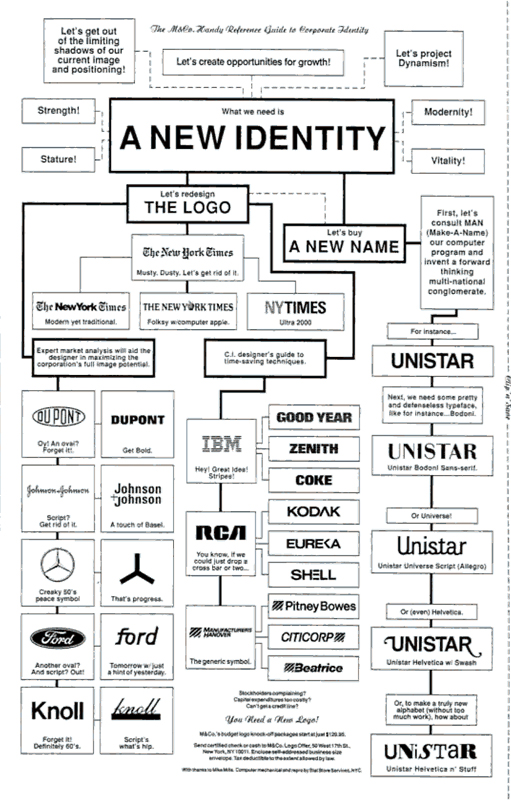
\includegraphics[width=.5\linewidth]{images/supplement/kalman}
\end{figure}

 \section{Классификация логотипов П. Моллерапа}
\label{app:mollerup}

\begin{figure}[ht]
  \centering
  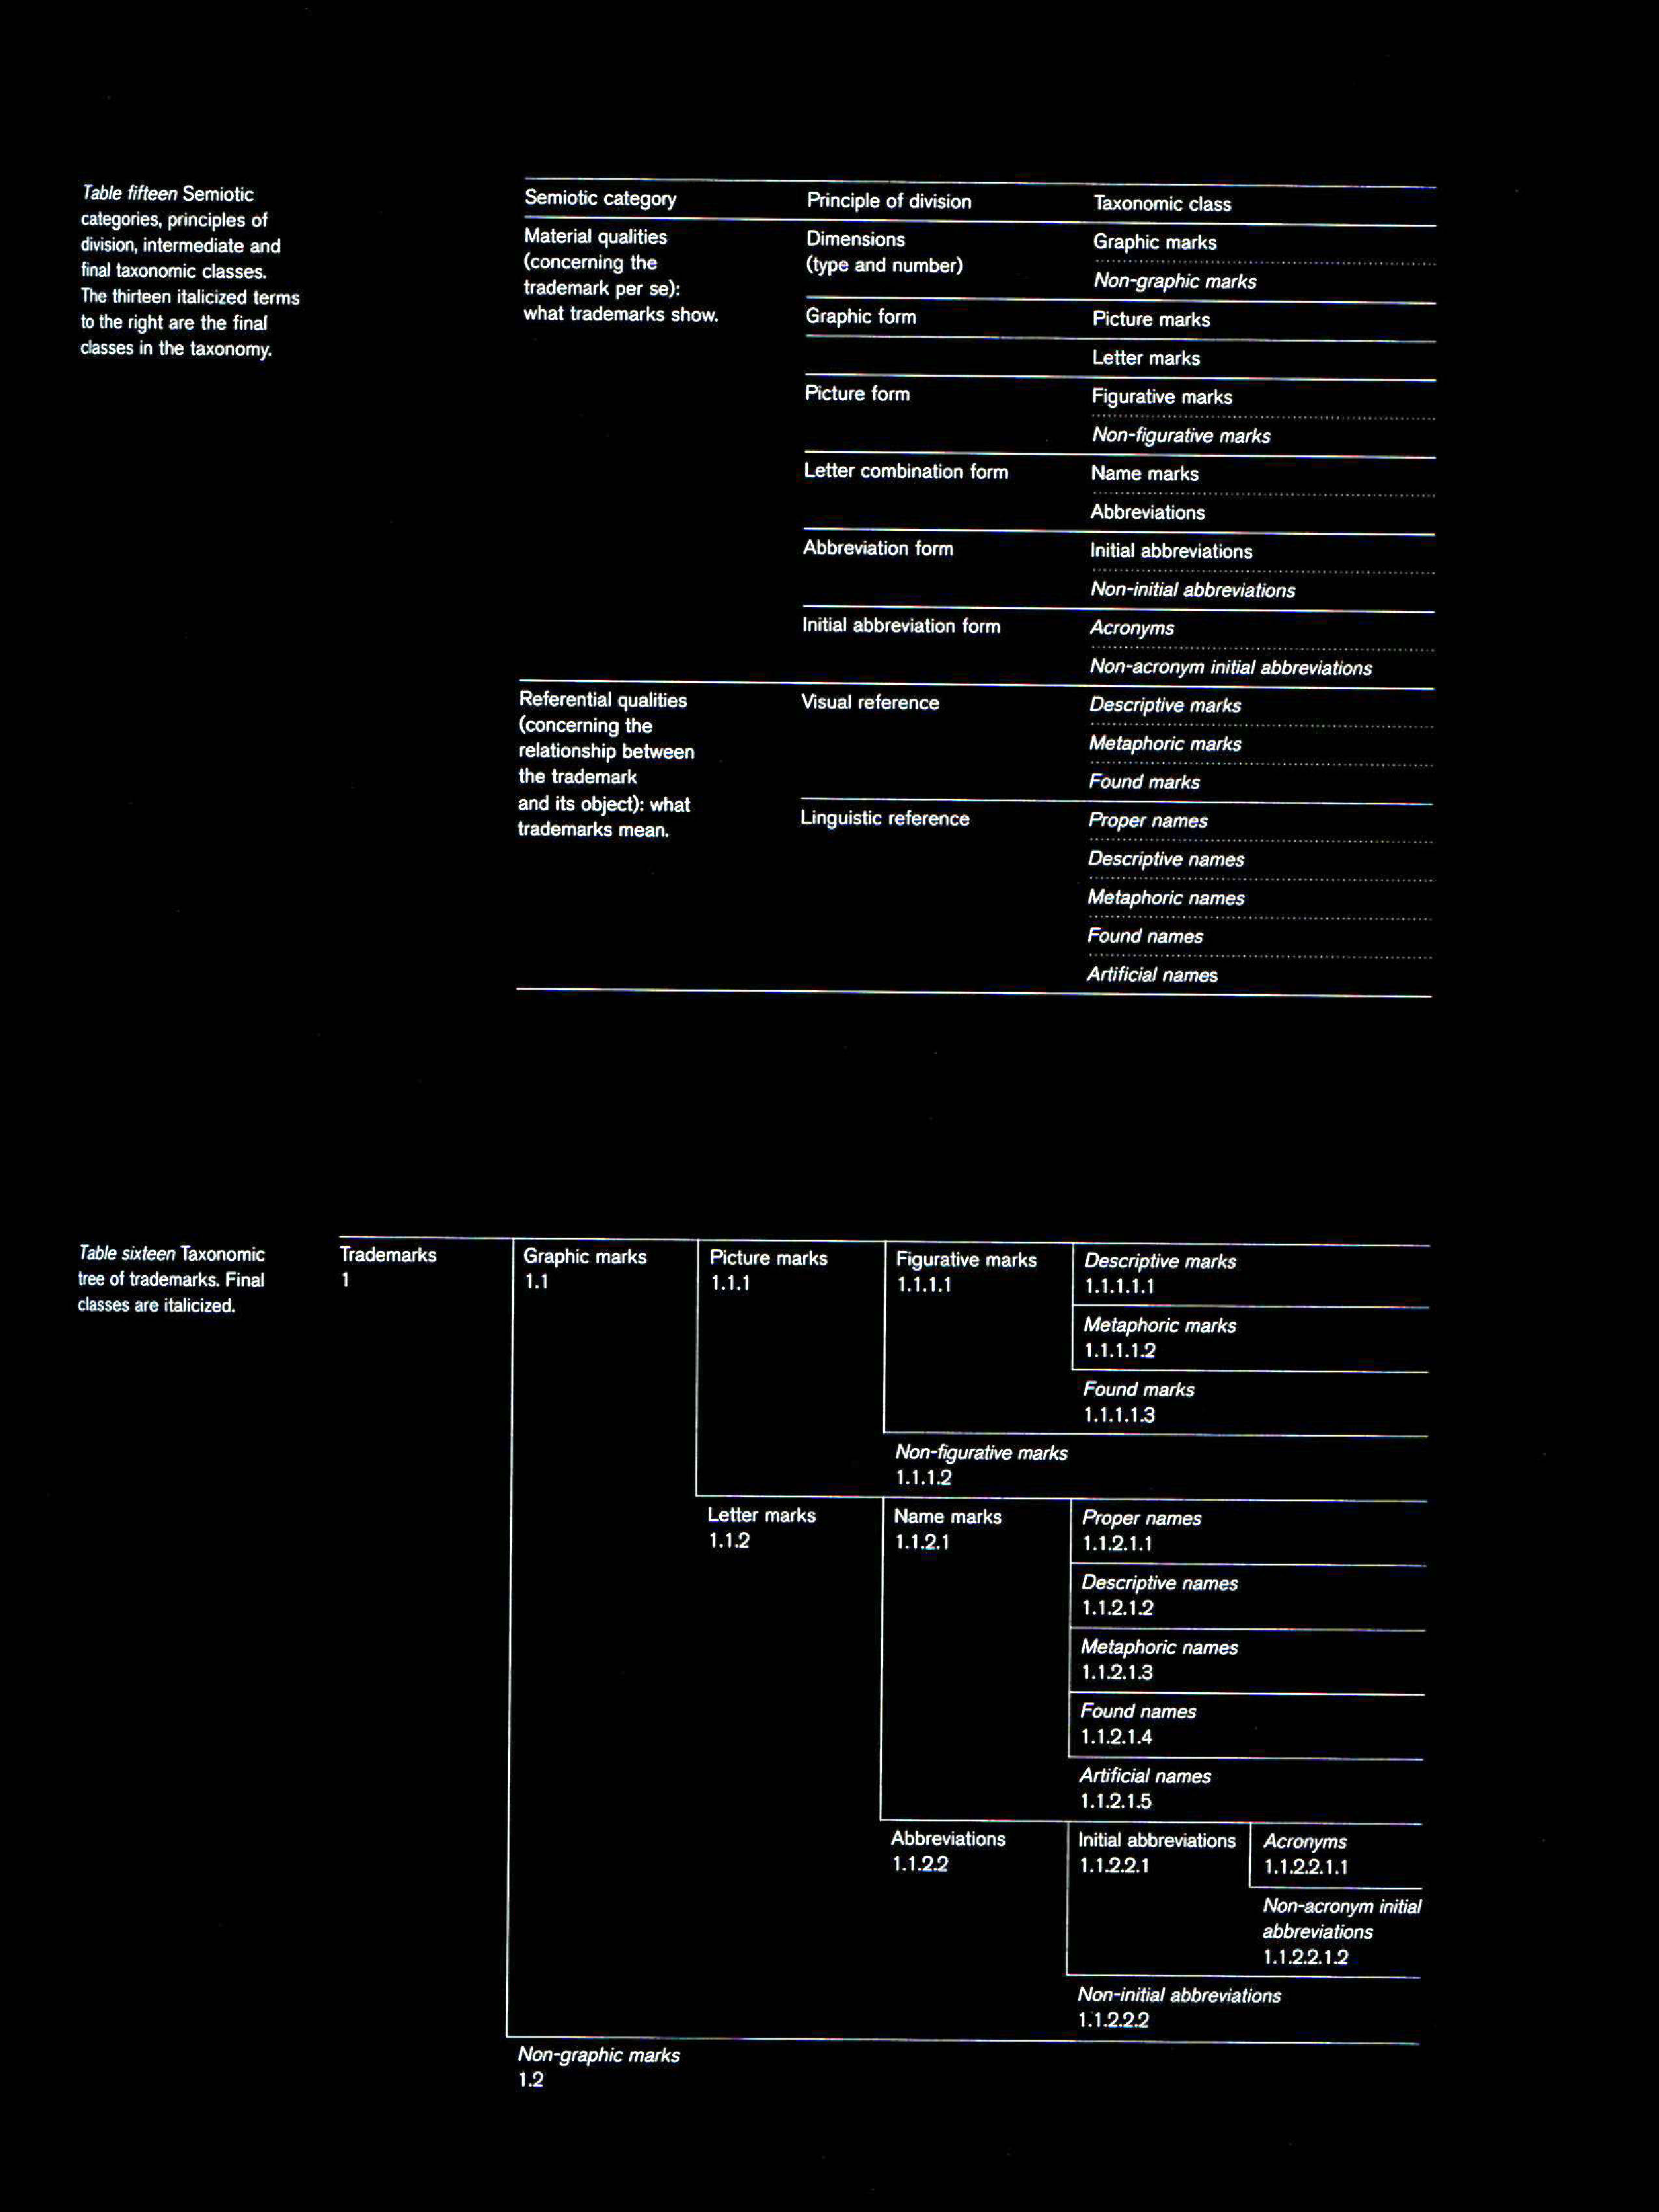
\includegraphics[width=.7\linewidth]{images/mollerup1}
  \caption{Классификация логотипов П. Моллерапа}
  \label{fig:mollerup1}
\end{figure}


 \section{Немецкие логотипы 1850--1950 гг.}
\label{app:german-trademarks}

\begin{figure}[ht]
  \centering
  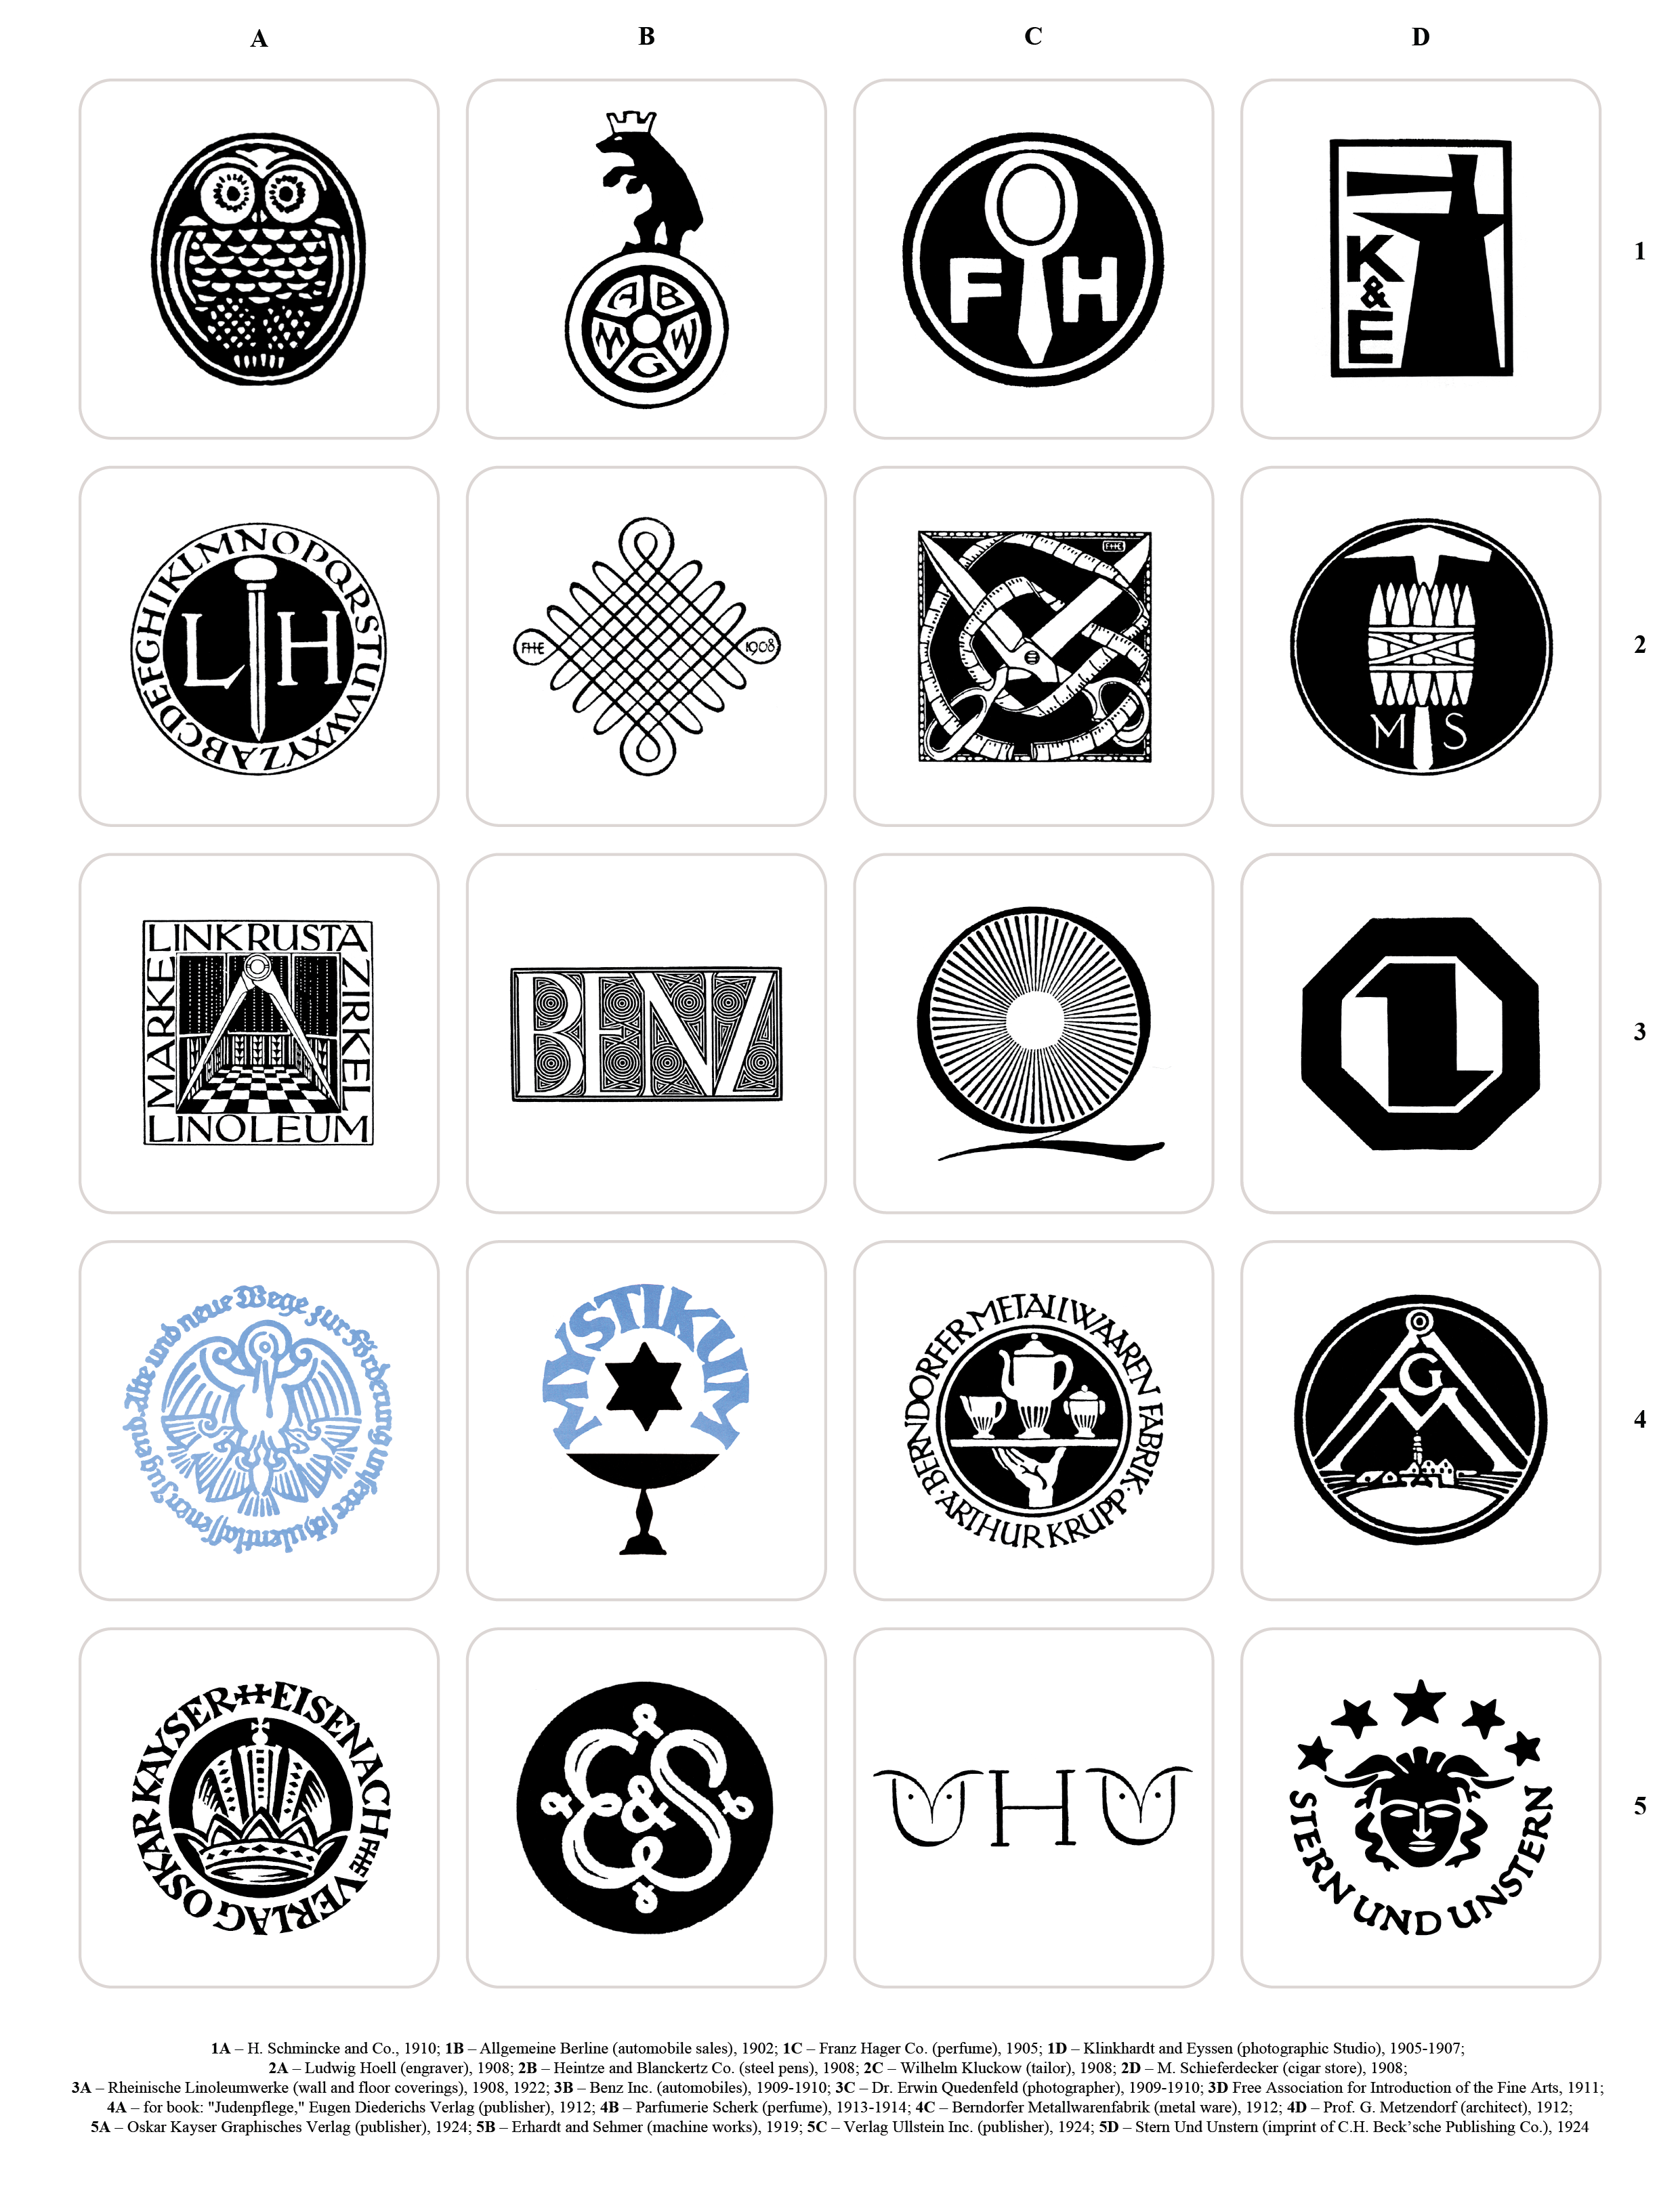
\includegraphics[width=.8\linewidth]{images/supplement/trademarks/german/emke}
  \caption{Логотипы Ф. Х. Эмке}
  \label{fig:trademarks:german:emke}
\end{figure}

\begin{figure}[ht]
  \centering
  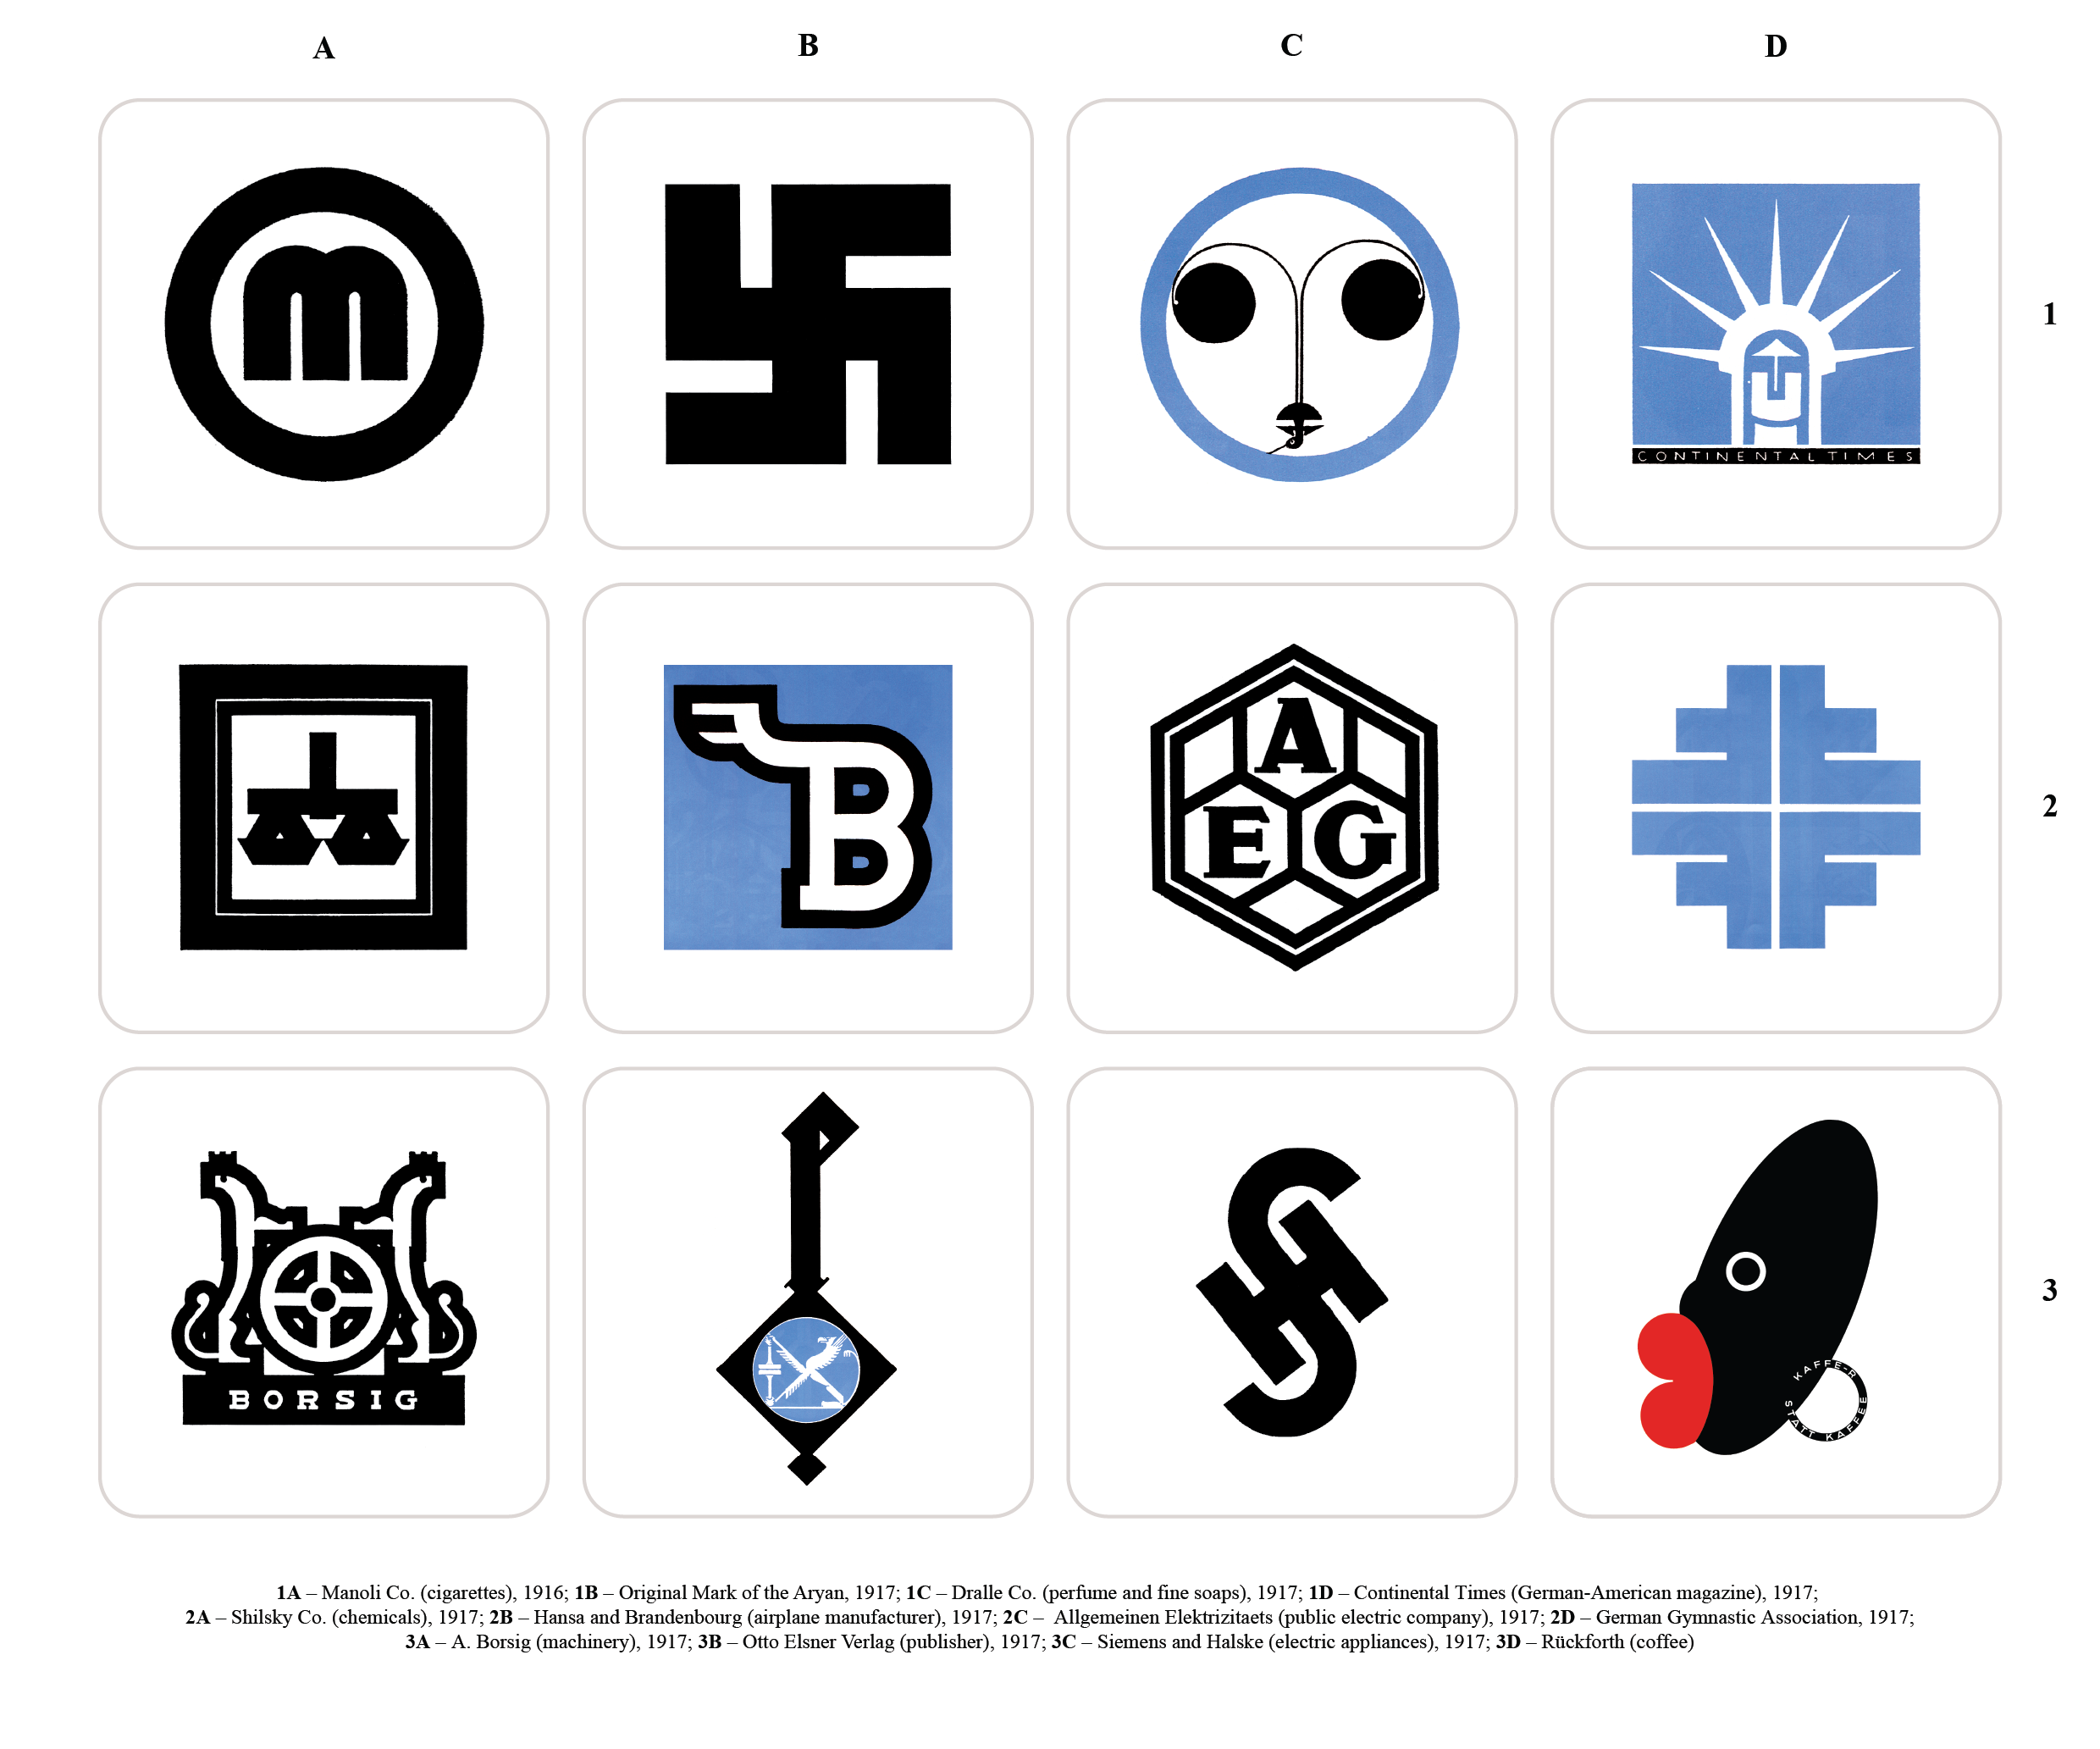
\includegraphics[width=.8\linewidth]{images/supplement/trademarks/german/dh}
  \caption{Логотипы В. Деффке и К.Э. Хинкефуса}
  \label{fig:trademarks:german:dh}
\end{figure}

\begin{figure}[ht]
  \centering
  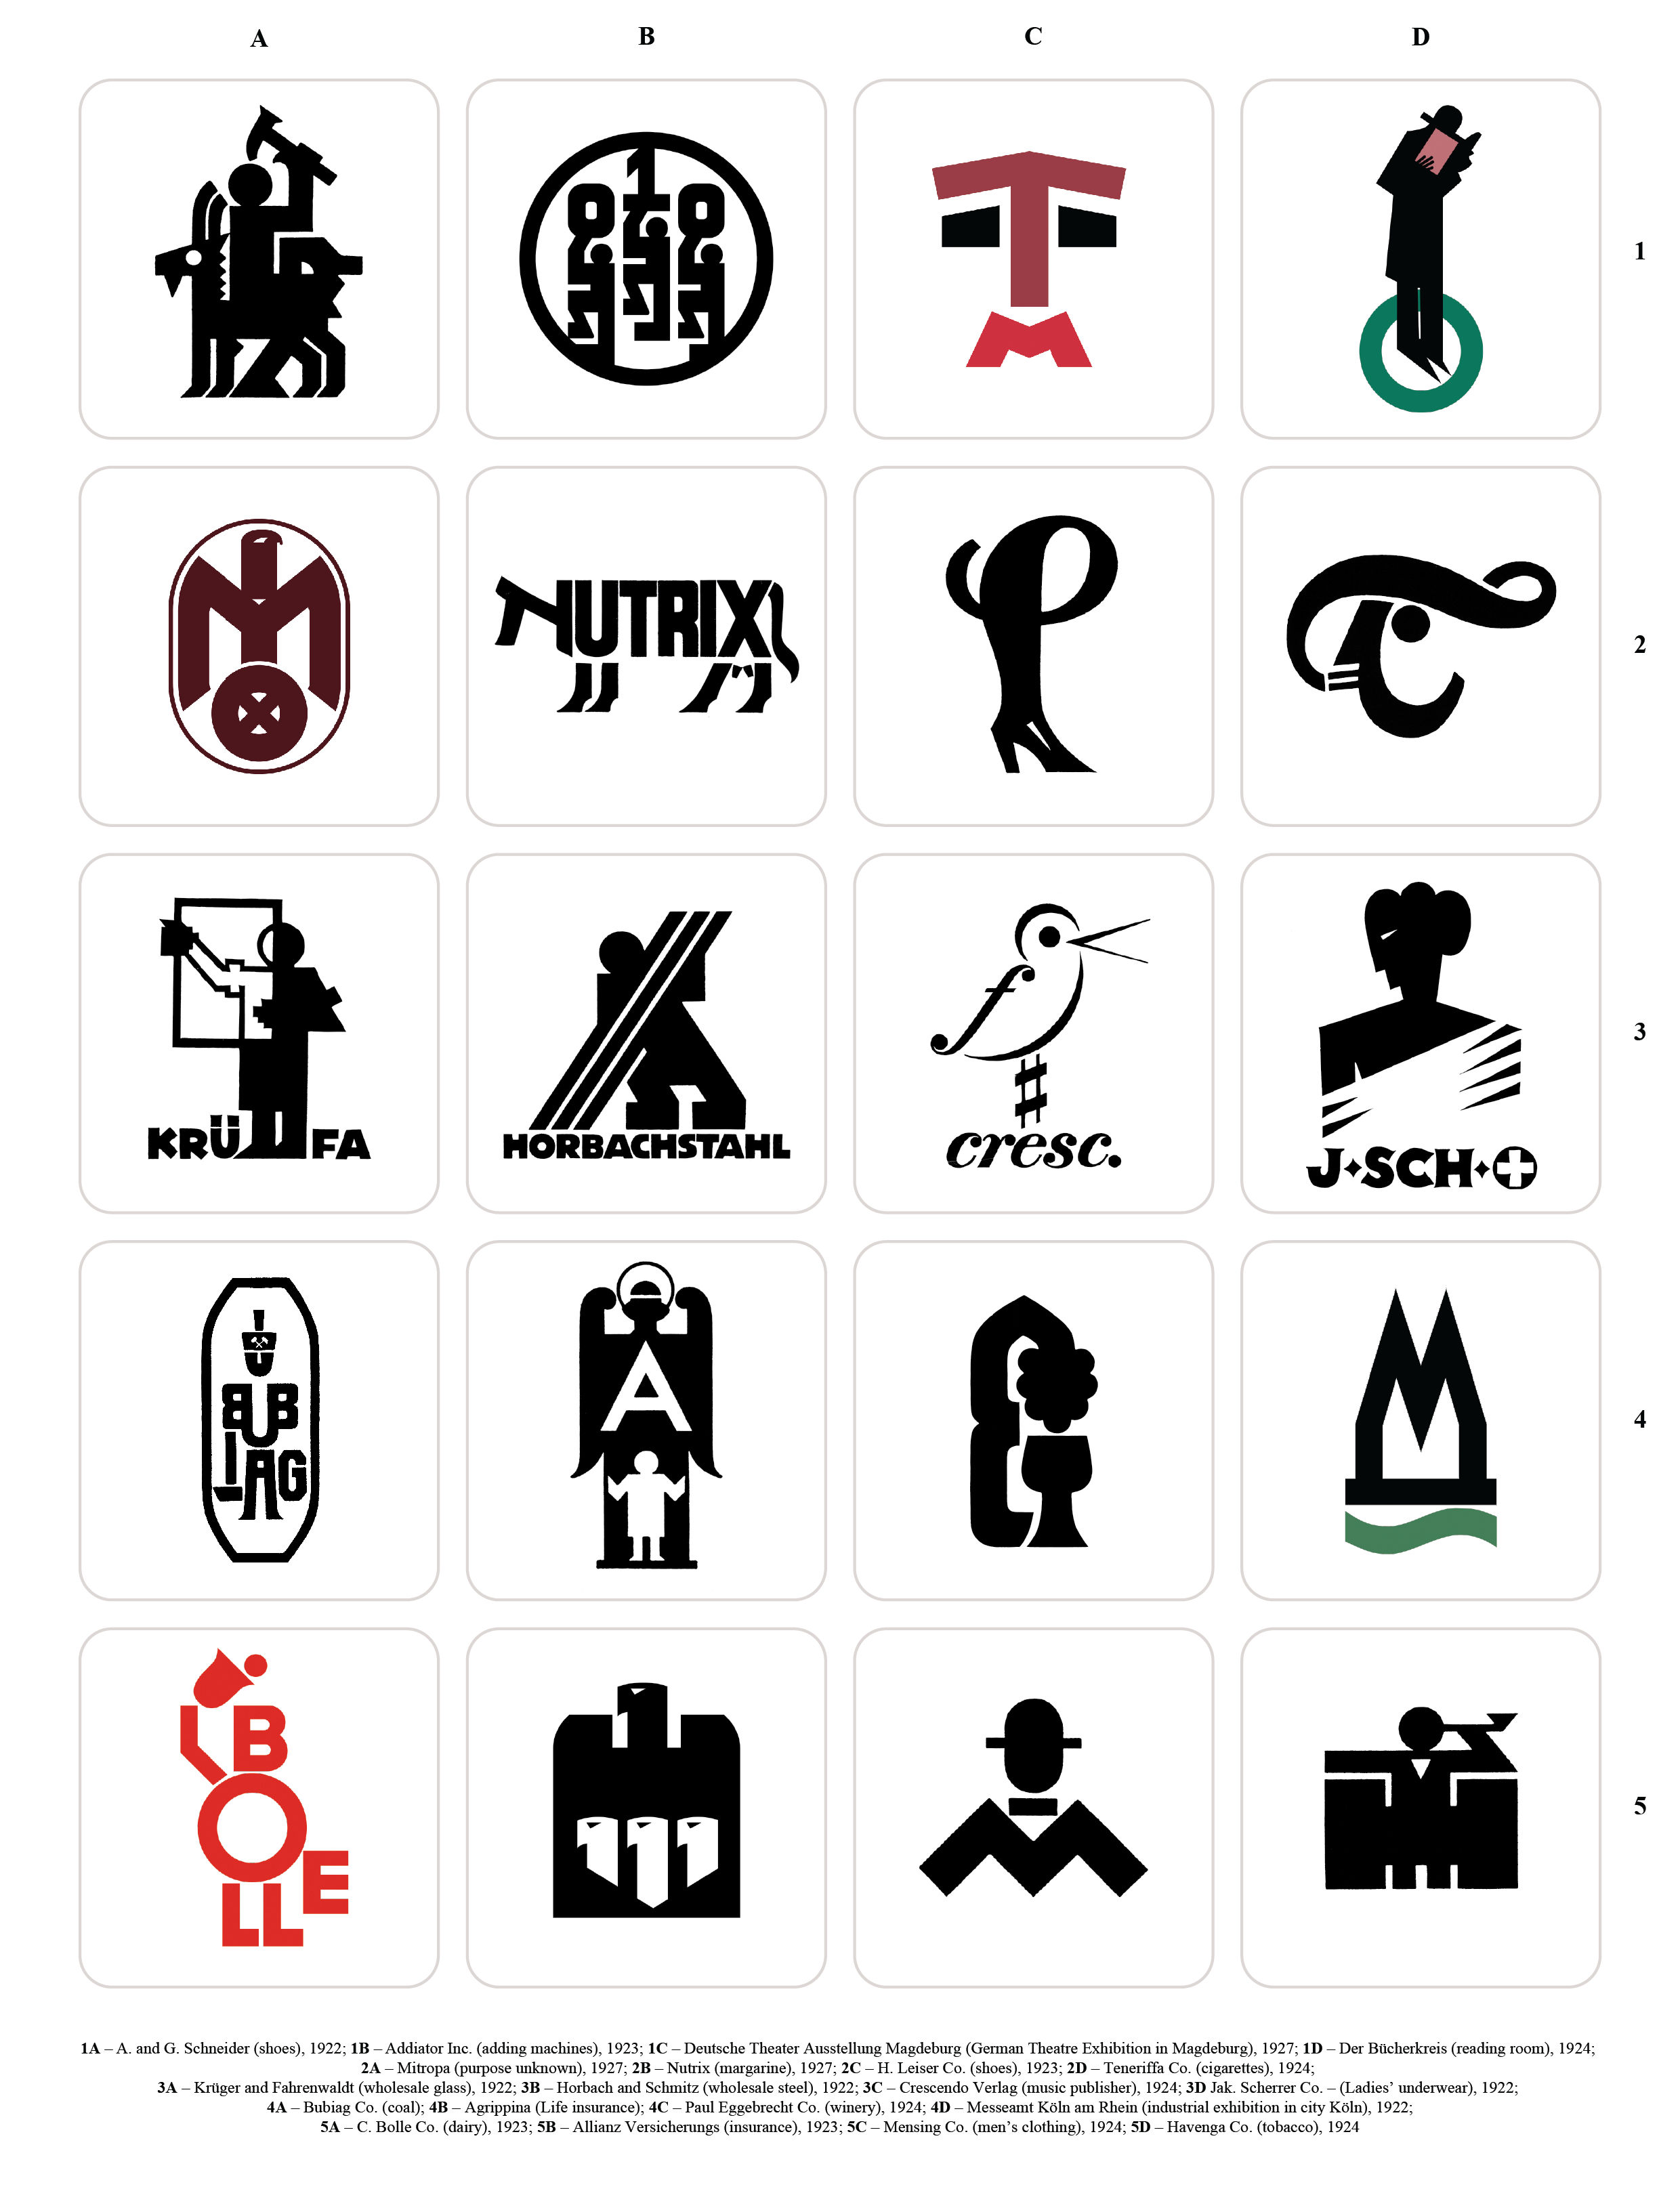
\includegraphics[width=.8\linewidth]{images/supplement/trademarks/german/shulpig}
  \caption{Логотипы К. Шульпига}
  \label{fig:trademarks:german:shulpig}
\end{figure}

 \section{Французские логотипы 1824--1974 гг.}
\label{app:french-trademarks}

\begin{figure}[h]
  \centering
  \begin{subfigure}{.45\textwidth}
    \centering
    
\includegraphics[width=.5\linewidth]{images/supplement/trademarks/french/1_1}
    \caption{Clothing S.A. Magasins A la ville de Babylone 1925 Paris}
    \label{fig:trademarks:french:1.1}
  \end{subfigure}\hfill
  \begin{subfigure}{.45\textwidth}
    \centering
    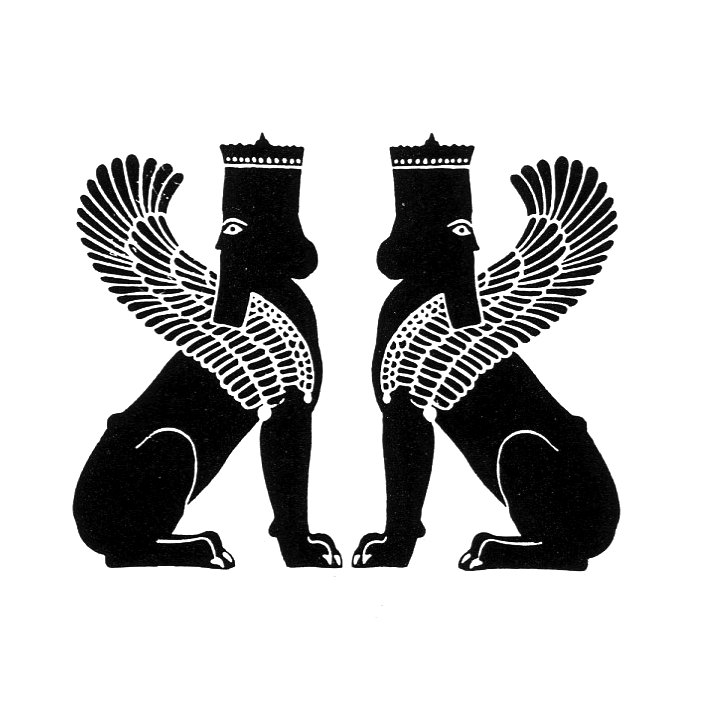
\includegraphics[width=.5\linewidth]{images/supplement/trademarks/french/1_2}
    \caption{All products Maison de l'Iran S. A. 1969 Paris}
    \label{fig:trademarks:french:1.2}
  \end{subfigure}

  \begin{subfigure}{.45\textwidth}
    \centering
    
\includegraphics[width=.5\linewidth]{images/supplement/trademarks/french/2_3}
    \caption{Beer Societe Anonyme Brasserie, Malterie Phoceenne 1902 Marseille}
    \label{fig:trademarks:french:2.3}
  \end{subfigure}\hfill
  \begin{subfigure}{.45\textwidth}
    \centering
    \includegraphics[width=.5\linewidth]{images/supplement/trademarks/french/2_4}
    \caption{Corsets M. Perrat J. 1905 Paris}
    \label{fig:trademarks:french:2.4}
  \end{subfigure}

  \begin{subfigure}{.45\textwidth}
    \centering
    \includegraphics[width=.5\linewidth]{images/supplement/trademarks/french/2_10}
    \caption{Pharmaceutical products Ste Etudes Scientifiques et Industrielles d'Ile-de-France 1946 Paris}
    \label{fig:trademarks:french:2.10}
  \end{subfigure}\hfill
  \begin{subfigure}{.45\textwidth}
    \centering
    \includegraphics[width=.5\linewidth]{images/supplement/trademarks/french/2_11}
    \caption{Butter, cheese Ste Laitiere Bonjean et Cie 1947 Sayat (Puy-de-Dome)}
    \label{fig:trademarks:french:2.11}
  \end{subfigure}
\end{figure}

\clearpage

\begin{figure}[h]
  \centering
  \begin{subfigure}{.45\textwidth}
    \centering
    \includegraphics[width=.5\linewidth]{images/supplement/trademarks/french/3_5}
    \caption{Tie collars, scarves, detachable collars MM. Bernard et Laucrene-Jeune 1876 Paris}
    \label{fig:trademarks:french:3.5}
  \end{subfigure}\hfill
  \begin{subfigure}{.45\textwidth}
    \centering
    \includegraphics[width=.5\linewidth]{images/supplement/trademarks/french/3_8}
    \caption{Corsets J. Chauvet 1894 Paris}
    \label{fig:trademarks:french:3.8}
  \end{subfigure}

  \begin{subfigure}{.45\textwidth}
    \centering
    \includegraphics[width=.5\linewidth]{images/supplement/trademarks/french/3_11}
    \caption{Paper Association Ouvriere <<Le Papier>> 1900 Paris (Seine)}
    \label{fig:trademarks:french:3.11}
  \end{subfigure}\hfill
  \begin{subfigure}{.45\textwidth}
    \centering
    \includegraphics[width=.5\linewidth]{images/supplement/trademarks/french/4_1}
    \caption{Brushes M. Loomer Charles 1885 Paris}
    \label{fig:trademarks:french:4.1}
  \end{subfigure}

  \begin{subfigure}{.45\textwidth}
    \centering
    \includegraphics[width=.5\linewidth]{images/supplement/trademarks/french/4_16}
    \caption{Airplanes Air-France 1934 Paris}
    \label{fig:trademarks:french:4.16}
  \end{subfigure}\hfill
  \begin{subfigure}{.45\textwidth}
    \centering
    \includegraphics[width=.5\linewidth]{images/supplement/trademarks/french/4_17}
    \caption{Airplanes Air-France 1935 Paris}
    \label{fig:trademarks:french:4.17}
  \end{subfigure}

  \begin{subfigure}{.45\textwidth}
    \centering
    \includegraphics[width=.5\linewidth]{images/supplement/trademarks/french/5_1}
    \caption{Threads MM. Verstracte 1862 Lille}
    \label{fig:trademarks:french:5.1}
  \end{subfigure}
  \begin{subfigure}{.45\textwidth}
    \centering
    \includegraphics[width=.5\linewidth]{images/supplement/trademarks/french/5_6}
    \caption{Tailoring, clothing Cendrillon S.A.R.L. 1948 Paris}
    \label{fig:trademarks:french:5.6}
  \end{subfigure}
\end{figure}

\clearpage

\begin{figure}[h]
  \centering
  \begin{subfigure}{.45\textwidth}
    \centering
    \includegraphics[width=.5\linewidth]{images/supplement/trademarks/french/5_41}
    \caption{Sewing threads Victor Saint-Leger 1881 Lille}
    \label{fig:trademarks:french:5.41}
  \end{subfigure}
  \begin{subfigure}{.45\textwidth}
    \centering
    \includegraphics[width=.5\linewidth]{images/supplement/trademarks/french/5_52}
    \caption{Brandy M. Cointreau Edouard 1899 Angers}
    \label{fig:trademarks:french:5.52}
  \end{subfigure}

  \begin{subfigure}{.45\textwidth}
    \centering
    \includegraphics[width=.5\linewidth]{images/supplement/trademarks/french/6_3}
    \caption{Hardware, polishes M. Ballain Jean 1942 Nantes}
    \label{fig:trademarks:french:6.3}
  \end{subfigure}
  \begin{subfigure}{.45\textwidth}
    \centering
    \includegraphics[width=.5\linewidth]{images/supplement/trademarks/french/6_4}
    \caption{Crushing, grinding, machines Ste de Construction Mecanique S.A.R.L. 1971 Ales (Gard)}
    \label{fig:trademarks:french:6.4}
  \end{subfigure}

  \begin{subfigure}{.45\textwidth}
    \centering
    \includegraphics[width=.5\linewidth]{images/supplement/trademarks/french/6_8}
    \caption{Salted, canned foods M. Borel Albert 1939 Nimes}
    \label{fig:trademarks:french:6.8}
  \end{subfigure}\hfill
  \begin{subfigure}{.45\textwidth}
    \centering
    \includegraphics[width=.5\linewidth]{images/supplement/trademarks/french/6_9}
    \caption{Wines M. Lanta Roger 1946 Artiguelouve (Pyrenees-Atlantiques)}
    \label{fig:trademarks:french:6.9}
  \end{subfigure}

  \begin{subfigure}{.45\textwidth}
    \centering
    \includegraphics[width=.5\linewidth]{images/supplement/trademarks/french/6_21}
    \caption{Threads M. Henri Borroughs 1860 Lille}
    \label{fig:trademarks:french:6.21}
  \end{subfigure}\hfill
  \begin{subfigure}{.45\textwidth}
    \centering
    \includegraphics[width=.5\linewidth]{images/supplement/trademarks/french/6_24}
    \caption{Mineral water Societe Anonyme Des Sources Sainte-Fontaine 1912 Paris}
    \label{fig:trademarks:french:6.24}
  \end{subfigure}
\end{figure}

\clearpage

\begin{figure}[h]
  \centering
  \begin{subfigure}{.45\textwidth}
    \centering
    \includegraphics[width=.5\linewidth]{images/supplement/trademarks/french/8_16}
    \caption{Foods Societe Guillemet Fils Lefebvre et Cie 1925 Niort}
    \label{fig:trademarks:french:8.16}
  \end{subfigure}\hfill
  \begin{subfigure}{.45\textwidth}
    \centering
    \includegraphics[width=.5\linewidth]{images/supplement/trademarks/french/8_25}
    \caption{Beer M. Boudinier Laron 1901 Elincourt}
    \label{fig:trademarks:french:8.25}
  \end{subfigure}

  \begin{subfigure}{.45\textwidth}
    \centering
    \includegraphics[width=.5\linewidth]{images/supplement/trademarks/french/8_34}
    \caption{Shoes M. Chemin Edouard 1927 Paris}
    \label{fig:trademarks:french:8.34}
  \end{subfigure}\hfill
  \begin{subfigure}{.45\textwidth}
    \centering
    \includegraphics[width=.5\linewidth]{images/supplement/trademarks/french/9_14}
    \caption{Musical records, publishing M. Roze Yves 1973 Paris}
    \label{fig:trademarks:french:9.14}
  \end{subfigure}

  \begin{subfigure}{.45\textwidth}
    \centering
    \includegraphics[width=.5\linewidth]{images/supplement/trademarks/french/9_21}
    \caption{Paints MM. Gaut, Balcan et Cie 1921 Paris}
    \label{fig:trademarks:french:9.21}
  \end{subfigure}\hfill
  \begin{subfigure}{.45\textwidth}
    \centering
    \includegraphics[width=.5\linewidth]{images/supplement/trademarks/french/10_5}
    \caption{Cigarette paper M. Duс Casimir 1889 Lyon}
    \label{fig:trademarks:french:10.5}
  \end{subfigure}

  \begin{subfigure}{.45\textwidth}
    \centering
    \includegraphics[width=.5\linewidth]{images/supplement/trademarks/french/10_51}
    \caption{Work clothes M. Pugeat Jean 1951 Villefranche-sur-Saone (Rhone)}
    \label{fig:trademarks:french:10.51}
  \end{subfigure}\hfill
  \begin{subfigure}{.45\textwidth}
    \centering
    \includegraphics[width=.5\linewidth]{images/supplement/trademarks/french/10_90}
    \caption{Cheese Fromageries Bel La Vache qui rit S.A. 1969 Paris}
    \label{fig:trademarks:french:10.90}
  \end{subfigure}
\end{figure}

\clearpage

\begin{figure}[h]
  \centering
  \begin{subfigure}{.45\textwidth}
    \centering
    \includegraphics[width=.5\linewidth]{images/supplement/trademarks/french/10_131}
    \caption{Brushes, toothbrushes M. Maurice Krupper 1927 Paris}
    \label{fig:trademarks:french:10.131}
  \end{subfigure}\hfill
  \begin{subfigure}{.45\textwidth}
    \centering
    \includegraphics[width=.5\linewidth]{images/supplement/trademarks/french/10_138}
    \caption{Champagne Champagne Heidsieck S.A. 1963 Reims}
    \label{fig:trademarks:french:10.138}
  \end{subfigure}

  \begin{subfigure}{.45\textwidth}
    \centering
    \includegraphics[width=.5\linewidth]{images/supplement/trademarks/french/11_6}
    \caption{Fresh vegetables Etab. R. Lapostolle 1958 Auxonne (Cote-d'Or)}
    \label{fig:trademarks:french:11.6}
  \end{subfigure}\hfill
  \begin{subfigure}{.45\textwidth}
    \centering
    \includegraphics[width=.5\linewidth]{images/supplement/trademarks/french/12_1}
    \caption{Foods, pasta M. Dumont Maurice 1917 Fleury-les-Aubrais (Loiret)}
    \label{fig:trademarks:french:12.1}
  \end{subfigure}

  \begin{subfigure}{.45\textwidth}
    \centering
    \includegraphics[width=.5\linewidth]{images/supplement/trademarks/french/12_2}
    \caption{Jewelry M. Gautie Emile 1898 Agen}
    \label{fig:trademarks:french:12.2}
  \end{subfigure}\hfill
  \begin{subfigure}{.45\textwidth}
    \centering
    \includegraphics[width=.5\linewidth]{images/supplement/trademarks/french/12_12}
    \caption{Candies, chocolates La Pie qui Chante 1959 Wattignies (Nord)}
    \label{fig:trademarks:french:12.12}
  \end{subfigure}

  \begin{subfigure}{.45\textwidth}
    \centering
    \includegraphics[width=.5\linewidth]{images/supplement/trademarks/french/15_9}
    \caption{Perfumes and cosmetic accessories S.A}
    \label{fig:trademarks:french:15.9}
  \end{subfigure}\hfill
  \begin{subfigure}{.45\textwidth}
    \centering
    \includegraphics[width=.5\linewidth]{images/supplement/trademarks/french/15_29}
    \caption{Cigars MM. Jorro freres 1902 Oran}
    \label{fig:trademarks:french:15.29}
  \end{subfigure}
\end{figure}

\begin{figure}[h]
  \centering
  \begin{subfigure}{.45\textwidth}
    \centering
    \includegraphics[width=.5\linewidth]{images/supplement/trademarks/french/15_47}
    \caption{Coffee S.A.R.L. Cafes Louis Jolivet 1962 Carcassonne}
    \label{fig:trademarks:french:15.47}
  \end{subfigure}\hfill
  \begin{subfigure}{.45\textwidth}
    \centering
    \includegraphics[width=.5\linewidth]{images/supplement/trademarks/french/20_4}
    \caption{Water-proof linens M. Turin Leon 1894 Paris}
    \label{fig:trademarks:french:20.4}
  \end{subfigure}

  \begin{subfigure}{.45\textwidth}
    \centering
    \includegraphics[width=.5\linewidth]{images/supplement/trademarks/french/20_7}
    \caption{Cigarette paper S.A. Nelle. du Valdor 1927 Paris}
    \label{fig:trademarks:french:20.7}
  \end{subfigure}\hfill
  \begin{subfigure}{.45\textwidth}
    \centering
    \includegraphics[width=.5\linewidth]{images/supplement/trademarks/french/20_21}
    \caption{Hair wax M. Tang Trong Hai 1952 Cholon-Cochinchine}
    \label{fig:trademarks:french:20.21}
  \end{subfigure}

  \begin{subfigure}{.45\textwidth}
    \centering
    \includegraphics[width=.5\linewidth]{images/supplement/trademarks/french/20_22}
    \caption{Tapioca cocoa M. Nestle Georges 1922 Vanves}
    \label{fig:trademarks:french:20.22}
  \end{subfigure}\hfill
  \begin{subfigure}{.45\textwidth}
    \centering
    \includegraphics[width=.5\linewidth]{images/supplement/trademarks/french/20_23}
    \caption{Strollers, cradles Babillage 1952 Paris}
    \label{fig:trademarks:french:20.23}
  \end{subfigure}

  \begin{subfigure}{.45\textwidth}
    \centering
    \includegraphics[width=.5\linewidth]{images/supplement/trademarks/french/21_32}
    \caption{Perfumes, cosmetics M. Baudercroux Paul 1954 Etang-la-ville (S et O)}
    \label{fig:trademarks:french:21.32}
  \end{subfigure}\hfill
  \begin{subfigure}{.45\textwidth}
    \centering
    \includegraphics[width=.5\linewidth]{images/supplement/trademarks/french/21_34}
    \caption{Candies Prevost et Cie 1894 Paris}
    \label{fig:trademarks:french:21.34}
  \end{subfigure}
\end{figure}

\begin{figure}[h]
  \centering
  \begin{subfigure}{.45\textwidth}
    \centering
    \includegraphics[width=.5\linewidth]{images/supplement/trademarks/french/21_45}
    \caption{Dresses M. Stroyman David 1925 Paris}
    \label{fig:trademarks:french:21.45}
  \end{subfigure}

  \begin{subfigure}{.45\textwidth}
    \centering
    \includegraphics[width=.5\linewidth]{images/supplement/trademarks/french/21_52}
    \caption{Clothing, fashion, feathers Simon Freres S}
    \label{fig:trademarks:french:21.52}
  \end{subfigure}

  \begin{subfigure}{.45\textwidth}
    \centering
    \includegraphics[width=.5\linewidth]{images/supplement/trademarks/french/21_53}
    \caption{Raincoats Fraenkel et Cie 1927 Paris}
    \label{fig:trademarks:french:21.53}
  \end{subfigure}
\end{figure}

 \section{Интервью автора с современными мировыми дизайнерами логотипов}

\subsection{Алан Ороноз}

\begin{description}
\item[Имя] Алан Ороноз
\item[Страна] Мексика
\item[Опыт работы] Графический дизайн (лого дизайн, брэндинг, иллюстрация, упаковка). 8 лет работы с клиентами со всего мира.
\end{description}

\textbf{Давайте начнем с общего вопроса: Что такое хороший логотип, по вашему мнению?}

Хороший логотип должен быть уникальным и запоминающимся. Я совершенно не считаю, что лого обязательно должно быть простым. Хорош тот логотип, которому удается передать суть компании. Рынок очень разнообразен. Аудитория, к которой обращен логотип неоднородна и восприимчива к разным визуальным элементам. Поэтому важно правильно оценить, что лучше всего подходит для определенного вида бизнеса.

\textbf{Что вы думаете по поводу брендинга стран? Будет ли в ближайшем будущем свой логотип у каждого места на земном шаре или это просто временный тренд?}

Я думаю, что глобализация совершенно изменила наше восприятие брэнда, и нация сегодня может рассматриваться как брэнд. Этот тренд переживал настоящий бум несколько лет назад, но я не думаю, что в будущем он станет глобальным. Однако некоторые страны возможно будут использовать его для стимулирования подъема экономики.


\textbf{Можно ли говорить о каком-то определенном национальном стиле логотипов?}

Национальные логотипы имеют тенденцию быть <<стилизовано современными>>. Такой стиль конечно же следует определенному тренду. Есть много схожего в том, что касается цвета, образов и даже шрифта.

\textbf{Согласны ли вы с тем, что логотип – это эмблема счастья в нашем потребительском обществе?}

Не сказал бы, что они эмблемы счастья, скорее – комфорта. Я думаю, что мир сегодня движется быстрее, мы находимся в состоянии стресса, и поэтому с каждым днем все более держимся за бренды, которые нам близки.

\textbf{Каково будущее лого дизайна? Как вы думаете, возможен ли сильный бренд без логотипа?}

Для меня бренд не работает без лого. Он, как верхушка айсберга. Совершенно очевидно, что если вы не увидите верхушку, то так никогда и не узнаете, что там, внизу, что-то есть. Я думаю, что лого дизайн будет существовать всегда. Он будет просто адаптироваться к своему времени. В дизайне есть тенденция к цикличности, и возможно через несколько лет минимализм устареет, но кто знает, что будет собой представлять следующий тренд?


\clearpage
\subsection{Георгий Бокуа}

\begin{description}
\item[Имя] Георгий Бокуа
\item[Страна] Грузия
\item[Опыт работы] --
\end{description}

\textbf{Давайте начнем с общего вопроса: Что такое хороший логотип, по вашему мнению?}

Основной ингредиент в хорошем логотипе – это чувство законченности и универсальности. Добавим несколько ложек умных графических решений, щепотку новаторства, талантливую смесь геометрических элементов и получится довольно вкусно!

\textbf{Что вы думаете по поводу брендинга стран? Будет ли в ближайшем будущем свой логотип у каждого места на земном шаре или это просто временный тренд?}

Мне кажется, что брендинг городов более привлекателен, чем брендинг стран. Для стран их национальные флаги и эмблемы важнее логотипов, придуманных для туристских целей. Если люди в мире станут дружелюбнее и гостепримнее, вот тогда возможно и брендинг наций будет более востребован.


\textbf{Можно ли говорить о каком-то определенном национальном стиле логотипов}

Универсальность – одно из лучших качеств логотипов сегодня, так как бренды становятся все более глобальными. Мне нравится грубоватый стиль голландских дизайнеров, которые выбирают нечто старое, грубоватое не только в графике, но и в моде и архитектуре.


\textbf{Согласны ли вы с тем, что логотип – это эмблема счастья в нашем потребительском обществе?}

Да, я с этим согласен. Думаю, что при виде логотипов любимых брендов, явно идет секреция гормонов счастья.


\textbf{Каково будущее лого дизайна? Как вы думаете, возможен ли сильный бренд без логотипа?}

Я думаю, что действительно талантливые логотипы в будущем будут выглядеть примерно также, как и великие логотипы сейчас. В большинстве таких логотипов используется одинаковая символика: крест, звезда, луна, стрела и т.д. Именно это делает их вневременными, вечными. За этими логотипами стоят великолепные продукты. Думаю, что даже плохой логотип может стать великим, если качество того, что он представляет действительно высоко.

Не уверен по поводу брендов без логотипов. Уже были попытки сделать это.
В целом же, если у вашего бренда есть имя, то, как бы вы его не писали, он получает айдентику. Однако, если имени нет, наверное это возможно.


\clearpage
\subsection{Петер Васвари}

\begin{description}
\item[Имя] Петер Васвари
\item[Страна] Венгрия
\item[Опыт работы] 10 лет
\end{description}

\textbf{Давайте начнем с общего вопроса: Что такое хороший логотип, по вашему мнению?}

Хороший логотип должен четко читаться в уменьшенном размере.


\textbf{Что вы думаете по поводу брендинга стран? Будет ли в ближайшем будущем свой логотип у каждого места на земном шаре или это просто временный тренд?}

Национальный брендинг сейчас довольно однообразен, но есть исключения, и это хорошо!


\textbf{Можно ли говорить о каком-то определенном национальном стиле логотипов?}

Национальные стили, конечно, существуют, например, логотипы Перу, Новой Зеландии и других стран.

\textbf{Согласны ли вы с тем, что логотип – это эмблема счастья в нашем потребительском обществе?}

Да, они действительно логотипы счастья, в том случае, если они грамотно визуально выполнены.


\textbf{Каково будущее лого дизайна? Как вы думаете, возможен ли сильный бренд без логотипа?}

Я надеюсь, что бренды сохранят четкую визуальную составляющую. К сожалению, сейчас наблюдается тенденция к упрощению лого дизайна. Например, просто круг или буква <<О>> уже могут представлять собой бренд.



\clearpage
\subsection{Шон О'Грейди}

\begin{description}
\item[Имя] Шон О'Грейди
\item[Страна] Ирландия
\item[Опыт работы] Издательское дело, спортивный брендинг, вывески, реклама, графический дизайн. Последние семь лет: лого дизайн и брендинг.
\end{description}

\textbf{Давайте начнем с общего вопроса: Что такое хороший логотип, по вашему мнению?}

Хороший логотип точно доносит до аудитории информацию, которую он продвигает.


\textbf{Что вы думаете по поводу брендинга стран? Будет ли в ближайшем будущем свой логотип у каждого места на земном шаре или это просто временный тренд?}

Национальный брендинг очень важен сегодня, особенно, если страна хочет развивать туризм. Каждая нация на земле имеет национальный флаг, что само по себе является наиональным брендом.


\textbf{Можно ли говорить о каком-то определенном национальном стиле логотипов?}

В качестве ирландского бренда обычно используется трилистник. Этой же роли зачастую служит арфа.


\textbf{Согласны ли вы с тем, что логотип – это эмблема счастья в нашем потребительском обществе?}

Я полагаю, что логотип должен представлять позитивный взгляд на компанию, поэтому, возможно, он и должен быть эмблемой сачстья.


\textbf{Каково будущее лого дизайна? Как вы думаете, возможен ли сильный бренд без логотипа?}

Лого, символы и другие эмблемы существуют уже столетия и будут существовать еще долго. Брендинг в последне время приобретает все более важный статус, что усиливает значимость  логотипа.


\clearpage
\subsection{Саймон Фроуз}

\begin{description}
\item[Имя] Саймон Фроуз
\item[Страна] Южная Африка
\item[Профессия] Графический дизайнер, творческий директор
\item[Опыт работы] 16 лет
\end{description}

\textbf{Давайте начнем с общего вопроса: Что такое хороший логотип, по вашему мнению?}

В случае успешного логотипа аудитория ощущает эмоциональную связь с брендом. Это может проявляться по-разному: доверие, желание, ощущение счастья. Если лого воплощает желаемые качества бренда, оно является успешным, на мой взгляд.


\textbf{Что вы думаете по поводу брендинга стран? Будет ли в ближайшем будущем свой логотип у каждого места на земном шаре или это просто временный тренд?}

Брендинг наций – это хорошо. Он помогает создать упрощенную визуальную карту, которую люди могут запомнить. Он может способствовать развитию туризма, экономическимх инвестиций и т.д. Брендинг наций словно отправляет послание от данной страны всему человечеству. Он может обладать огромной силой в объединении людей, что и произошло в Африке.

Брендированию в той или иной форме (визуальной или какой-либо иной) подвергается все, поэтому весьма
логично, что нации стремятся к созданию индивидуальных
(URL: \url{http://www.southafrica.net/za/en/landing/visitor-home}) или коллективных
(URL: \url{http://europa.eu/geninfo/atoz/en/index_1_en.htm}) брендов. Я полагаю, что в будущем все нации
будут иметь лого, ибо у всех нас есть желание принадлежать к чему-то большему, чем мы сами.

\textbf{Можно ли говорить о каком-то определенном национальном стиле логотипов?}

Да, в разных странах всегда существуют уникальные культурные влияния на дизайн. Однако из-за современной глобализации и благодаря средствам коммуникации наблюдается все большее слияние стилей, и тренды растпространены более широко, чем прежде. Становится все труднее определить страну создания определенного логотипа. И тем не менее, многие развивающиеся государства пытаются создать четкую национальную идентичность, вызванную стремлением отличаться от других. А такие страны, как США, зачастую демонстрируют в лого дизайне  сильное чувство патриотизма.


\textbf{Согласны ли вы с тем, что логотип – это эмблема счастья в нашем потребительском обществе?}

Я с этим не согласен. Логотипы изображают самые разные эмоции. Счастье – одна из них, но не единственная. Есть примеры успешных логотипов, символизирующих негатиные эмоции, такие как страх и ненависть.

\textbf{Каково будущее лого дизайна?}

Иллюстрированные, фотографические, анимационные, 3-D, голлографические логотипы. Мне кажется, что логотипы станут более сложными. Становится все труднее и труднее создать оригинальный простой логотип. С появлением цифровых технологий правила игры изменились. Традиционное требование к логотипу четко чиаться в одном цвете и маленьком размере со временем исчезнет.

\textbf{Как вы думаете, возможен ли сильный бренд без логотипа?}

Бренд какое-то время может существовать без логотипа, но в нашей природе распределять вещи по категориям и давать им названия, так что со временем кто-то наделит бренд визуальной репрезентацией. Но возможно, если печатные средсвта информации когда-то окончательно устареют, бренд сможет быть представлен, например, лишь звуком. Или вообще одной идеей!

\end{appendices}
\end{document}
